% TODO: normalize IVT for definite integrands does not exist (but Mean Value Theorem for definite integrands does)
\documentclass{article}
%\usepackage[top=30pt,left=30pt,right=30pt]{geometry}
\usepackage[german,english]{babel}
\usepackage[utf8]{inputenc}
\usepackage{algpseudocode}
\usepackage{algorithm}
\usepackage{graphicx}
\usepackage{caption}
\usepackage{subcaption}
\usepackage{amsmath}
\usepackage{amssymb}
\usepackage{enumitem}
\usepackage{amsthm}
\usepackage{bbm}
\usepackage{pxfonts}
\usepackage{wasysym}
\usepackage{framed}
\usepackage{mdframed}
\usepackage{xcolor}
\usepackage{makeidx}
\usepackage{csquotes}
\usepackage[pdfborder={0 0 0}]{hyperref}
\usepackage{stmaryrd}
\usepackage{titlesec}
\titleformat{\paragraph}{\normalfont\itshape}{}{}{}

\newtheorem{theorem}{Theorem}  \numberwithin{theorem}{section}
\newtheorem{problem}{Problem}  \numberwithin{problem}{section}
\newtheorem{example}{Example}  \numberwithin{example}{section}
\newtheorem*{hypothesis}{Hypothesis}%  \numberwithin{hypothesis}{section}
\newtheorem{definition}{Definition}  \numberwithin{definition}{section}
\newtheorem{lemma}{Lemma}  \numberwithin{lemma}{section}
\newtheorem*{claim}{Claim}%  \numberwithin{claim}{section}
\newtheorem{remark}{Remark}  \numberwithin{remark}{section}
\newtheorem*{corollary}{Corollary}%  \numberwithin{corollary}{section}
\newtheorem{proposition}{Proposition}  \numberwithin{proposition}{section}

\algnewcommand{\algorithmicgoto}{\textbf{go to}}%
\algnewcommand{\Goto}[1]{\algorithmicgoto~\ref{#1}}%
\algrenewcommand{\algorithmiccomment}[1]{\hskip2em$\triangleright$ {\footnotesize #1}}

% definitions
\newcommand{\drawing}[1]{%
 \begin{figure}[t]
  \begin{center}
   \includegraphics{#1}
  \end{center}
 \end{figure}
}
\newcommand{\pic}[2]{%
 \begin{figure}[t]
  \begin{center}
   \includegraphics{#1}
   \caption{#2}
  \end{center}
 \end{figure}
}
\newcommand{\set}[1]{\left\{#1\right\}}
\newcommand{\setdef}[2]{\left\{\left.#1\,\middle|\,#2\right.\right\}}
\newcommand{\angel}[1]{\left\langle#1\right\rangle}
\newcommand{\norm}[1]{\left\|#1\right\|}
\newcommand{\card}[1]{\left|#1\right|}
\newcommand{\given}[1]{\textbf{Given.} #1\par}
\newcommand{\find}[1]{\textbf{Find.} #1\par}
\newcommand{\dateref}[1]{%
  \begin{mdframed}[backgroundcolor=gray!10,innerbottommargin=0pt,innertopmargin=0pt]
    \paragraph{\textit{$\downarrow$ This lecture took place on #1.}}%
  \end{mdframed}%
}
\newcommand{\exist}{\;\exists\,}
\newcommand{\fall}{\;\forall\,}
\newcommand{\noproof}[1]{A proof for Theorem~\ref{#1} is not provided.}
\newcommand{\vectwo}[2]{\begin{pmatrix} #1 \\ #2 \end{pmatrix}}
\newcommand{\bectwo}[2]{\begin{bmatrix} #1 \\ #2 \end{bmatrix}}
\makeatletter
\newcommand{\xRightarrow}[2][]{\ext@arrow 0359\Rightarrowfill@{#1}{#2}}
\makeatother

\newcommand{\mtn}{(\mu\times\nu)} % mu times nu

\DeclareMathOperator{\rank}{rank}
\DeclareMathOperator{\detm}{det}
\DeclareMathOperator{\perm}{det}
\DeclareMathOperator{\sign}{sign}
\DeclareMathOperator{\degree}{deg}
\DeclareMathOperator{\prop}{probability}
\DeclareMathOperator{\argmax}{argmax}
\DeclareMathOperator{\argmin}{argmin}
\DeclareMathOperator{\vol}{vol}  % volume
\DeclareMathOperator{\sinc}{sinc}
\DeclareMathOperator*{\bigtimes}{\vartimes}

\makeatletter
\providecommand*{\dotcup}{%
  \mathbin{%
    \mathpalette\@dotcup{}%
  }%
}
\newcommand*{\@dotcup}[2]{%
  \ooalign{%
    $\m@th#1\cup$\cr
    \hidewidth$\m@th#1\cdot$\hidewidth
  }%
}
\makeatother


% metadata
\title{
  Analysis 2 \\
  \large{Lecture notes, University (of Technology) Graz} \\
  based on the lecture by Wolfgang Ring
}
\date{\today}
\author{Lukas Prokop}

% settings
\parindent0pt
\setlength{\parskip}{0.4\baselineskip}
%\setcounter{tocdepth}{2}

\makeindex

\begin{document}
\maketitle
\tableofcontents

\dateref{2018/03/06}

\section{Mathematical Redux and topological fundamentals}
\subsection{Metric}

\index{Metric}
\index{Distance function}
\index{Metric space}
\begin{definition}
  Let $X \neq \emptyset$ be a set. We define a map $d: X \times X \to [0,\infty)$.
  $d$ should behave like a geometrical distance. We require $\forall x, y, z \in X$:
  \begin{itemize}
    \item $d(x, y) = d(y, x)$ [called \emph{symmetry}]
    \item $d(x, y) = 0 \iff x = y$ [called \emph{positive definiteness}]
    \item $\forall x,y,z \in X: d(x, z) \leq d(x, y) + d(y, z)$ [called \emph{triangle inequality}]
  \end{itemize}
  Then $d$ is called \emph{metric} or \emph{distance function} on $X$.
  $(X, d)$ is called \emph{metric space}.
\end{definition}

\begin{example}
  \begin{itemize}\hfill{}
    \item $X \subseteq \mathbb C$, $d(x, y) = \card{x - y}$.
          It satisfies $\card{x - z} \leq \card{x - y} + \card{y - z}$
    \item $X \subseteq \mathbb R^n$, $\norm{x - y} = \angel{x - y, x - y}^{\frac12}$
  \end{itemize}
\end{example}

\begin{claim}
  \[ \angel{x, y} = \sum_{i=1}^n x_i y_i \]
  \[ \norm{x} = \angel{x,x}^{\frac12} = \sqrt{\sum_{i=1}^n x_i^2} \]
  \[ \norm{x} = \sqrt{x_1^2 + x_2^2} \]
  The triangle inequality holds: $\norm{x+y} \leq \norm{x} + \norm{y}$.
\end{claim}

\begin{proof}
  \begin{align*}
    \norm{x + y}^2
      &= \angel{x+y, x+y} \\
      &= \angel{x,x} + \angel{x,y} + \angel{y,x} + \angel{y,y} \\
      &= \norm{x}^2 + 2\angel{x,y} + \norm{y}^2 \\
      &\leq \norm{x}^2 + 2 \norm{x} \norm{y} + \norm{y}^2  & [\text{by Cauchy-Schwarz ineq.}] \\
      &= (\norm{x} + \norm{y})^2 \\
    \norm{x - y}^2
      &= \angel{x - y, x - y} \\
      &= \norm{x}^2 - 2\angel{x,y} + \norm{y}^2 \\
    \norm{x + y}^2 + \norm{x - y}^2
      &= 2 \left(\norm{x}^2 + \norm{y}^2\right)
  \end{align*}
\end{proof}

\subsection{Cauchy-Schwarz inequality}

\begin{theorem}[Cauchy-Schwarz inequality]
  \[ \card{\angel{x, y}} \leq \norm{x} \norm{y} \]
\end{theorem}
\begin{proof}
  \[ 0 \leq \angel{x - \lambda y, x - \lambda y} = \norm{x}^2 - 2\lambda \angel{x, y} + \lambda^2 \norm{y}^2 \qquad \forall \lambda \in \mathbb R \]
  \[
    \lambda \coloneqq \frac{\angel{x, y}}{\norm{y}^2}
    \implies 0 \leq \norm{x}^2 - 2 \frac{\card{\angel{x, y}}^2}{\norm{y}^2} + \frac{\card{\angel{x, y}}^2}{\norm{y}^4} \cdot \norm{y}^2
  \]
  \[
    \iff 0 \leq \norm{x}^2 - \frac{\card{\angel{x, y}}^2}{\norm{y}^2}
    \iff \frac{\card{\angel{x, y}}^2}{\norm{y}^2} \leq \norm{x}^2
    \iff \card{\angel{x, y}}^2 \leq \norm{x}^2 \cdot \norm{y}^2
  \]
\end{proof}

\subsection{Euclidean norm}

\index{Euclidean norm}
\index{Norm}
\index{Normed vector space}
\begin{definition}
  $\norm{x} = \sqrt{\sum_{i=1}^n x_i^2}$ is called \emph{Euclidean norm} (length) of vector $x \in \mathbb R^n$. $\norm{x} = \angel{x, x}^{\frac12}$.
  It satisfies:
  \begin{enumerate}
    \item $\norm{\lambda x} = \card{\lambda} \norm{x} \forall x \in \mathbb R^n, \lambda \in \mathbb R$
    \item $\norm{x} = 0 \iff x = 0$ in $\mathbb R^n$
    \item $\norm{x + y} \leq \norm{x} + \norm{y}$
  \end{enumerate}
  In general:
    Let $V$ be a vector space over $\mathbb R$.
    A map $\norm\cdot$,
      which assigns every vector $x$ a non-negative real number satisfying the properties above,
      is called \emph{norm on $V$}.
    Then $(V, \norm\cdot)$ is called a \emph{normed vector space}.
\end{definition}

Let $X \subseteq \mathbb R^n$ ($V$ is a normed vector space), then $d(x, y) = \norm{x - y}$ is a metric on $X$.
\[ \norm{y - x} = \norm{(-1) (x - y)} = \card{-1} \cdot \norm{x - y} = \norm{x - y} \]
\[ d(x, y) = 0 \iff \norm{x - y} = 0 \iff x - y = 0 \iff x = y \]
\[ d(x, z) = \norm{z - x} = \norm{z - y + y - x} \leq \norm{z - y} + \norm{y - x} = d(z, y) + d(y, x) \]

\subsection{Metric space}

\begin{example}[metric space]
  Distance is not a norm.
  Consider an area in $\mathbb R^3$.

  $d(x,y)$ is the shortest path, connecting $x$ and $y$ in $X$.
  See Figure~\ref{img:example-r3}.

  \begin{figure}
    \begin{center}
      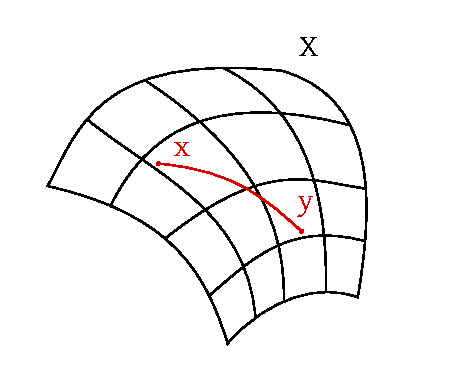
\includegraphics{img/01_example.pdf}
      \caption{Example in $\mathbb R^3$. The red line illustrates the shortest path, which is not necessarily \enquote{straight}.}
      \label{img:example-r3}
    \end{center}
  \end{figure}
\end{example}

\begin{example}[French railway]
  All connections between two cities pass through Paris except one city is Paris.
\end{example}

\begin{example}
  $X = \mathbb R^2$. Let $p \in \mathbb R^2$ be fixed.
  \[
    d(x, y) = \begin{cases}
      \card{x - y}                & \text{if } x, y, p \text{ are on one line} \\
      \card{x - p} + \card{p - y} & \text{if } x, y, p \text{ are not on one line}
    \end{cases}
  \]
\end{example}

\subsection{Open sets, convergence and accumulation points}

Now we put some terminology into the context of a metric space.
$(X, d)$ is a metric space.

\index{Open sphere}
\begin{definition}
  Let $x \in X$, $r \geq 0$.
  $K_r(x)$ is an \emph{open sphere} with radius $r$ at center $x$.
  \[ K_r(x) \coloneqq \setdef{z \in X}{d(x, z) < r} \]
\end{definition}

\begin{definition} $\overline{K_r(x)}$ is a closed sphere with center $x$ and radius $r$.
  \[ \overline{K_r(x)} \coloneqq \setdef{z \in X}{d(x, z) \leq r} \]
\end{definition}

\index{Convergence}
\index{Cauchy sequence}
\begin{definition}[Sequences in $X$]
  Let $(x_n)_{n\in\mathbb N}$ be a sequence in $X$ (hence, $\forall n \in \mathbb N: x_n \in X$)
  \begin{enumerate}
    \item $(x_n)_{n\in\mathbb N}$ is called \emph{convergent} and limit $x \in X$ if
      \[ \forall \varepsilon > 0 \exists N \in \mathbb N: n \geq N \implies d(x_n, x) < \varepsilon \]
      Denoted as $\lim_{n\to\infty} x_n = x$.
    \item $(x_n)_{n\in\mathbb N}$ is a Cauchy sequence if
      \[ \forall \varepsilon > 0 \exists N \in \mathbb N: n, m \geq N \implies d(x_n, x_m) < \varepsilon \]
  \end{enumerate}
\end{definition}

\begin{claim}
  Every convergent sequence is also a Cauchy sequence.
\end{claim}

\begin{proof}
  Let $(x_n)_{n\in\mathbb N}$ be convergent with limit $x$. Let $\varepsilon > 0$ be arbitrary.
  Because $(x_n)_{n\in\mathbb N}$ is convergent, there exists $N \in \mathbb N$ such that $n \geq N \implies d(x_n, x) < \frac{\varepsilon}{2}$.
  Now let $n,m \geq N$. Then,
  \[ d(x_n, x_m) \leq \underbrace{d(x_n, x)}_{< \frac{\varepsilon}2} + \underbrace{d(x, x_m)}_{< \frac\varepsilon2} < \varepsilon \]
\end{proof}

\index{Complete metric space}
\begin{definition}
  $(X, d)$ is called \emph{complete metric space} if every Cauchy sequence in $X$ is also convergent (has a limit).
\end{definition}

$\mathbb R$ is complete. $\mathbb R^n$ is also complete. $\mathbb Q \subseteq \mathbb R$ is incomplete.

\index{Accumulation point}
\begin{definition}
  Let $(x_n)_{n\in\mathbb N}$ be a sequence of $X$. $x$ is called \enquote{accumulation point} (\foreignlanguage{german}{dt. H\"aufungspunkt}) of the sequence if
  $\forall \varepsilon > 0: K_{\varepsilon}(x)$ contains infinitely many sequence elements.
\end{definition}

\dateref{2018/03/08}

$(X, d)$ is called \emph{metric space}.

\[ d(x,y) =0 \iff x = y \]
\[ \forall x,y \in X: d(x,y) = d(y,x) \]
\[ d(x,z) \leq d(x,y) + d(y,z) \forall x,y,z \in X \]

\subsection{Norm}

\index{Norm}
Let $V$ be a vector space. $\norm{\cdot}$ is called \emph{norm on $V$}.
\[ \norm{x} = 0 \iff x = 0 \]
\[ \forall \lambda \in \mathbb R, \mathbb C: \forall x \in V: \norm{\lambda x} = \card{\lambda} \norm{x} \]
\[ \forall x,y,z \in V: \norm{x + y} \leq \norm{x} + \norm{y} \]

Let $X \subseteq V$ be a subset of normed vector space $V$.
Then $X$ is a metric space with $d(x,y) = \norm{x - y}$.

\index{Euclidean norm}
For $V = \mathbb R^n$. Then
\[ \norm{x} = \left(\sum_{i=1}^n x_i^2\right)^{\frac12} \]
is a norm on $\mathbb R^n$. $\norm{x}_2$ is called \emph{Euclidean norm on $\mathbb R^n$}.

Other norms in $\mathbb R^n$:
\[ \norm{x}_{\infty} = \max\setdef{\card{x_i}}{i = 1,\dots,n} \]
\[ \norm{x}_1 = \sum_{i=1}^n \card{x_i} \]
for $1 \leq p < \infty$.
\[ \norm{x}_p = \left(\sum_{i=1}^n \card{x_i}^p\right)^{\frac1p} \]
e.g. $\norm{x}_1$ in $\mathbb R^2$

\begin{figure}[!ht]
  \begin{center}
    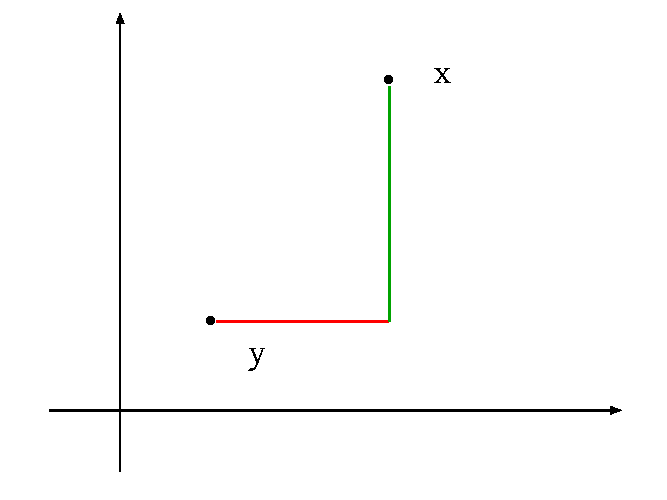
\includegraphics{img/02_1norm.pdf}
    \caption{Visualizing $\norm{x}_1$, the Manhattan norm. You can think of walking the distance along the x-axis combined with the distance along the y-axis.}
    \label{img:1norm}
  \end{center}
\end{figure}

\index{Manhattan metric}
\[ \norm{x - y} = \card{x_1 - y_1} + \card{x_1 - y_2} \]
is the so-called \emph{Manhattan metric}.

The concepts \enquote{subsequence}, \enquote{final element of a sequence}, \enquote{reordering of a sequence} correspond one-by-one to metric spaces.

\index{Accumulation point}
\begin{definition}[Accumulation point]
  Let $(X_n)_{n\in\mathbb N}$ be a sequence in $X$. $x \in X$ is called \emph{accumulation point of sequence $X$}
  if $\forall \varepsilon > 0$ the sphere $K_{\varepsilon}(x)$ contains infinitely many elements.
\end{definition}

\begin{lemma}
  $x \in X$ is accumulation point of sequence $(x_n)_{n\in\mathbb N}$
  if and only iff there exists a subsequence $(x_{n_k})_{k \in \mathbb N}$ such that
  $x = \lim_{k\to\infty} x_{n_k}$.
\end{lemma}

\begin{proof}
  See Analysis 1 course
\end{proof}

%\subsection{Sets in metric spaces}
\subsection{Contact point}

Let $B \subseteq X$ and $X$ is a metric space. Then $B$ with $d$ is a metric space itself.

\index{Contact point}
\begin{definition}
  Let $B \subseteq X$ and $x \in X$. We say, $x$ is a \emph{contact point of $B$}
  if $\forall \varepsilon > 0: K_{\varepsilon}(x) \cap B \neq \emptyset$.

  [ $y \in X$ is not a contact point of $B \iff \exists \varepsilon > 0: K_{\varepsilon}(y) \cap B = \emptyset$ ]

  See Figure~\ref{img:cp}.
\end{definition}

\begin{figure}
  \begin{center}
    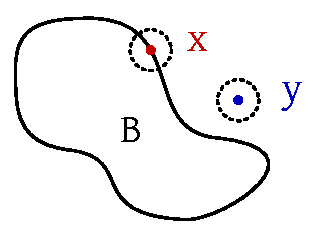
\includegraphics{img/03_contact_point.pdf}
    \caption{Contact points in set $B$}
    \label{img:cp}
  \end{center}
\end{figure}

We let $\overline{B} = \setdef{x \in X}{x \text{ is contact point of } B}$.

$\overline{B}$ is called closed hull of $B$.

$B$ is called closed if $B = \overline{B}$, hence, every contact point is also element of $B$.

\begin{remark}
  Because $\forall x \in B$ holds $K_r(x) \cap B \supseteq \set{x} \forall r > 0$ is $x$ always contact point of $B$.
  Also $B \subseteq \overline{B}$ (always)
\end{remark}

\begin{lemma}
  $x$ is contact point of $B \iff \exists (x_n)_{n\in\mathbb N}$ with $x_n \in B$ and $\lim_{n\to\infty} x_n = x$.
\end{lemma}
\begin{proof}
  Let $x$ be a contact point of $B$.

  Direction $\Rightarrow$:
  Because $K_{\frac1n}(x) \cap B \neq \emptyset$, choose $X_n \in K_{\frac1n}(x) \cap B$.
  The sequence $(x_n)_{n\in\mathbb N}$ has property $d(x_n, x) < \frac1n$.
  Let $\varepsilon > 0$ be arbitrary. Choose $N \in \mathbb N$ sch that $N > \frac1\varepsilon$ (consider the Archimedean axiom).
  Then for $n \geq N$, $d(x_n, x) < \frac1n \leq \frac1N < \varepsilon$, hence $\lim_{n\to\infty} x_n = x$.

  Direction $\Leftarrow$:
  Let $x = \lim_{n\to\infty} x_n$ and $x_n \in B$.
  Let $\varepsilon > 0$ be arbitrary and $N \in \mathbb N$ such that $d(x_n, x) < \varepsilon \forall n \geq N$.
  Then $d(x_N, x) < \varepsilon$, hence
  \[ x_N \in \underbrace{K_{\varepsilon}(x) \cap B}_{\neq \emptyset} \]
  So $x$ is contact point of $B$.
\end{proof}

\begin{lemma}
  $\forall B \subseteq X: \overline{B} = \overline{\overline{B}}$.
  So $\overline{B}$ is closed in itself.
\end{lemma}
\begin{proof}
  Show that $x \in \overline{B}$.

  Let $x \in \overline{\overline{B}}$
  $\iff \forall \varepsilon > 0: K_{\varepsilon}(x) \cap \overline{B} \neq \emptyset$.
  Therefore let $\varepsilon > 0$ be arbitrary and $x \in \overline{\overline{B}}$.

  Show that $K_{\varepsilon}(x) \cap B \neq \emptyset$.

  Because $x \in \overline{\overline{B}}: \exists y \in \overline{B}: y \in K_{\frac\varepsilon2}(x)$.
  Because $y \in \overline{B}: \exists z \in B: z \in K_{\frac\varepsilon2}(y)$. Hence,
  \[ d(z,x) \leq \underbrace{d(z,y)}_{<\frac\varepsilon2} + \underbrace{d(y,x)}_{<\frac\varepsilon2} < \varepsilon \]
  so $z \in K(x,\varepsilon) \cap B$. So $x$ is contact point of $B \implies x \in \overline{B}$.
\end{proof}

\begin{lemma}
  \label{lemma4}
  Let $X$ be a metric space.
  \begin{itemize}
    \item
      $A_i \subseteq X$ be closed $\forall i \in I$.
      Then $A = \bigcap_{i \in I} A_i = \setdef{x \in X}{x \in A_i \forall i \in I}$
      is closed itself.
    \item
      $A_1, \dots, A_n \subseteq X$ are closed. Then $\bigcup_{k=1}^n A_k$ is closed in $X$.
    \item
      $\varphi$ is closed, $X$ is closed.
  \end{itemize}
\end{lemma}

\begin{proof}
  See Analysis 1 course.
\end{proof}

\begin{definition} % definition 8
  Let $x \in X$ be called accumulation point of set $B \subseteq X$ if $\forall \varepsilon > 0: (K_{\varepsilon}(x) \setminus \set{x}) \cap B \neq \emptyset$.
\end{definition}

\begin{remark}
  Accumulation \emph{points} only exist in the context of \emph{sets}.
  Accumulation \emph{values} only exist in the context of \emph{sequences}.

  For example $(+1, -1, +1, -1, +1, \dots)$ has accumulation \emph{values} $+1$ and $-1$.
\end{remark}

\begin{lemma}
  Let $x \in X$ be accumulation point on $B \iff$ every sphere $K_{\varepsilon}(x)$ contains infinitely many points of $B$.
\end{lemma}
\begin{proof}
  Direction $\Leftarrow$ is trivial.

  Direction $\Rightarrow$:
  Choose $x_1 \in (K_1(x) \setminus \set{x}) \cap B$, hence $x_1 \neq x$, $x_1 \in B$ and $d(x_1, x) < 1$.
  Let $r_1 = 1$.

  Inductive: choose $r_n = \min(\frac1n, d(x_{n-1}, x))$ and $x_n \in (K_{r_n}(x) \setminus \set{x}) \cap B$.
  Then $d(x_n, x) > 0$ (because $x_n \neq x$) where $d(x_n, x) < r_n < \frac1n$.
  \[ 0 < d(x_n, x) < \frac1n \]
  Furthermore, $d(x_n, x) < r_n \leq d(x_{n-1}, x)$.
  So $x_n \neq x_{n-1}$.

  Inductive: $x_n \neq x_{n-1} \neq x_{n-2} \neq \dots \neq x_1$.
  Now consider arbitrary $\varepsilon > 0$ and $N$ large enough such that $\frac1N < \varepsilon$.

  Then $\forall n \geq N: 0 < d(x_n, x) < \frac1n \leq \frac1N < \varepsilon$.
  So $K_{\varepsilon}(x) \cap B$ contains infinitely many points $x_N, x_{N+1}, x_{N+2}, \dots$.
\end{proof}

\index{Inner point}
\begin{definition} % definition 9
  Let $U \subseteq X$ and $x \in U$.
  We say $x$ is an \emph{inner point of $U$} if $\exists r > 0: K_r(x) \subseteq U$.
  We let $\mathring{U} = \setdef{x \in U}{x \text{ is inner point of } U}$ and call it \emph{interior of $U$} (dt. \foreignlanguage{german}{offenen Kern von $U$} or \foreignlanguage{german}{das Innere von $U$}).
  $O \subseteq X$ is called \emph{open} (open set), if every point $x \in O$ is also an inner point of $O$.
  Hence $\mathring{O} = O$. Compare with image~\ref{img:inner}.
\end{definition}

\begin{figure}[t]
  \begin{center}
    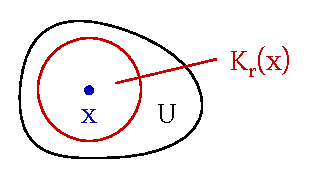
\includegraphics{img/04_inner_point.pdf}
    \caption{$x$ is an inner point of $U$ if $\exists r > 0: K_r(x) \subseteq U$}
    \label{img:inner}
  \end{center}
\end{figure}

\begin{example}
  Let $K_r(x)$ with $r > 0$ be an open sphere in $X$.
  Then $K_r(x)$ is an open set in $X$.
  Compare with image~\ref{img:opensp}.
\end{example}

\begin{proof}
  Why? Let $y \in K_r(x)$. Show that $y$ is an inner point of the sphere.
  $d(y,x) = s < r$. Define $r' = r - s > 0$.

  Claim: $K_r'(y) \subseteq K_r(x)$.

  Let $z \in K_{r'}(y)$, hence $d(z, y) < r'$. Then,
  \[ d(z, x) \leq \underbrace{d(x, y)}_{< r'} + \underbrace{d(y, z)}_{= s} < r' + s = r \]
  So $z \in K_r(x)$ and therefore $K_{r'}(y) \subseteq K_r(x)$.
\end{proof}

\begin{figure}[t]
  \begin{center}
    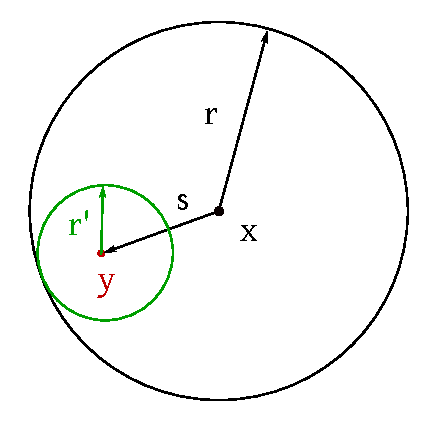
\includegraphics{img/05_open_sphere.pdf}
    \caption{Let $K_r(x)$ with $r>0$ be an open sphere in $X$. Then $K_r(x)$ is an open set in $X$.}
    \label{img:opensp}
  \end{center}
\end{figure}


\begin{lemma}
  Let $U \subseteq X$ be arbitrary. Then $\mathring{U} \subseteq X$ is an open set in $X$.
\end{lemma}
\begin{proof}
  Let $x \in \mathring{U}$. Hence $x$ is an inner point of $U$.
  Show that $x$ is an inner point of $\mathring{U}$, also $\exists r > 0: K_r(x) \subseteq \mathring{U}$.

  Because $x \in \mathring U$, $r > 0$ exists: $K_r(x) \subseteq U$.
  Claim: Every point $y \in K_r(x)$ is also an inner point of $U$.
  Obvious (previous example), because $r' > 0$ exists such that
  $K_{r'}(y) \subseteq K_r(x) \subseteq U$ so $y \in \mathring U$ and $K_r(x) \subseteq \mathring U$.
\end{proof}

\begin{theorem}
  \label{saetzchen1}
  Let $X$ be a metric space.
  \[ A \subseteq X \text{ is closed in $X$ } \iff O = X \setminus A = A^C \text{ is open} \]
\end{theorem}

\begin{proof}
  Let $A$ be closed and $O + A^C$. We choose $x \in O$ and show that $x$ is in the interior of $O$.

  Assume the opoosite.
  \[ \forall \varepsilon > 0: \underbrace{\neg \left(K_{\varepsilon}(x) \subseteq O\right)}_{\iff K_{\varepsilon}(x) \cap O^C \neq \emptyset} \]
  where $O^C = A$.

  Direction $\Leftarrow$.
  So $x$ is contact point of $A$.
  Because $A$ is closed, $x \in A$.
  This contradicts with $x \in O = A^C$. Thus $O$ is open.

  Direction $\Rightarrow$.
  Let $O = A^C$ be open and let $x$ be a contact point of $A$. Show that $x \in A$.

  Assume the opposite, hence $x \in A^C = O$ and $O$ is open.
  So $\exists r > 0: K_r(x) \subseteq O$, so $K_r(x) \cap A = \diameter$ where $A = O^C$.
  Hence $x$ is not a contact point of $A$.

  So every contact point of $A$ is also an element of $A$ and $A$ is closed.
\end{proof}

\begin{theorem}
  \label{satz2}
  Let $X$ be a metric space. Then,
  \begin{itemize}
  	\item
  	  If $O_i \subseteq X$ is open in $X$ $\forall i \in I$.
  	  Then also $O = \bigcup_{i \in I} O_i$ is open in $X$.
  	\item
  	  If $O_1, O_2, \dots, O_n$ is open in $X$, then $\bigcap_{k=1}^n O_k$ is open in $X$.
  	\item
  	  $X$ is open, $\emptyset$ is open.
  \end{itemize}
\end{theorem}

\begin{proof}
  By Lemma~\ref{lemma4}, Theorem~\ref{saetzchen1} and De Morgan's Laws:
  \[ \left(\bigcup_{i \in I} A_i\right)^C = \bigcap_{i in I} A_i^C \]
\end{proof}

\subsection{Topology}

\index{Topology}
\index{Topological spcae}
\begin{definition}
  Given a set $X$. If a subset $T \subseteq \mathcal P(X)$ is defined
  such that the elements $O \in T$ (hence $O \subseteq X$) satisfy the conditions of Theorem~\ref{satz2},
  then $T$ is called \emph{topology on $X$}.
  $(X, T)$ is called topological space.

  The sets $O \in T$ are called \emph{open sets} in terms of $T$.
  The complements $A = O^C$ for $O \in T$ are called \emph{closed sets}.
\end{definition}

\begin{definition}
  Let $x \in U \subseteq X$. We claim that $U$ is a neighborhood of $x$,
  if $r > 0$ exists such that $x \in K_r(X) \subseteq U$

  See Figure~\ref{img:neigh}
\end{definition}

\begin{figure}
  \begin{center}
    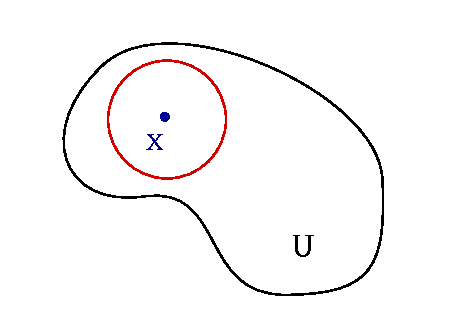
\includegraphics{img/06_neighborhood.pdf}
    \caption{Neighborhood of $x$}
    \label{img:neigh}
  \end{center}
\end{figure}

\begin{remark}
  $O \subseteq X$ is open iff $O$ is neighborhood of every point $x \in O$.
\end{remark}

\begin{definition}
  Let $X$ and $Y$ be metric spaces and $x_0 \in X$.
  Let $f: X \to Y$ be given. We say $f$ is continuous in $x_0$ if
  \[ \forall \varepsilon > 0 \exists \delta > 0: \forall x \in X: d_X(x, x_0) < \delta \implies d_Y(f(x), f(x_0)) < \varepsilon \]
  Here, $d_X$ is a metric on $X$ and $d_Y$ is a metric on $Y$.
\end{definition}

\dateref{2018/03/13}

\begin{theorem} % Satz 3
  \label{satz3t}
  Let $X$ and $Y$ be metric spaces. $f: X \to Y$. Let $x_0 \in X$ be given.
  Then the following statements are equivalent:
  \begin{enumerate}
    \item $f$ is continuous in $x_0$
    \item For every neighborhood $V$ of $y_0 = f(x_0)$ it is given that $f^{-1}(V)$ is a neighborhood of $x_0$
    \item For every sequence $(x_n)_{n \in \mathbb N}$ with $\lim_{n\to\infty} f(x_n) = f(x_0)$
  \end{enumerate}
\end{theorem}

\begin{proof}
  See Analysis 1.
\end{proof}

\index{Continuity on a set}
\begin{definition} % Definition 12
  Let $f: X \to Y$ be called continuous on $X$, if $f$ is continuous in every point $x_0 \in X$.
\end{definition}

\begin{theorem} % Satz 4
  Let $f: X \to Y$ be given.
  Then $f$ is continuous on $X \iff \forall \text{ open } O \subseteq Y: U = f^{-1}(O) \text{ open in } X$.
\end{theorem}

\begin{remark}
  This characterization of continuity also works in topological spaces.
\end{remark}

\begin{proof}
  Direction $\Rightarrow$.

  Let $f$ be continuous in $X$ and let $O \subseteq Y$ be open. Let $U = f^{-1}(O)$ and choose $x_0 \in U$. Then $f(x_0) \in O$, hence $O$ is a neighborhood of $f(x_0)$. By Theorem~\ref{satz3t}~(b), it follows that $U = f^{-1}(O)$ is a neighborhood of $x_0$.

  Hence, $U$ is neighborhood of every of its points, hence open in $X$.

  Direction $\Leftarrow$.

  Let the preimages of open sets be open and $x_0 \in X$ and $y_0 = f(x_0)$.
  Let $V$ be a neighborhood of $y_0 = f(x_0)$, hence $\exists \varepsilon > 0: K_{\varepsilon}(f(x_0)) \subseteq V$. Because $K_{\varepsilon}(f(x_0))$ is an open set, $f^{-1}(K_{\varepsilon}(f(x_0))) \in x_0$ is open in $X$.

  Therefore, there exists $\delta > 0$ such that $K_{\delta}(x_0) \subseteq f^{-1}(K_{\varepsilon}(f(x_0))) \subseteq f^{-1}(V)$. Hence, $f^{-1}(V)$ is a neighborhood of $x_0$. Then by Theorem~\ref{satz3t}~(b), it follows that $f$ is continuous in $x_0$ (chosen arbitrarily). Hence $f$ is continuous on $X$.
\end{proof}

\subsection{Variations of continuity notions}
\subsubsection{Uniform continuity}

\index{Uniformly continuous}
\begin{definition} % Definition 13
  Let $f: X \to Y$ be given.
  We call \enquote{f uniformly continuous on $X$} if
  \[
  	\forall \varepsilon > 0 \exists \delta > 0:
  	\forall x, y \in X \land d_X(x,y) < \delta \implies d_Y(f(x), f(y)) < \varepsilon
  \]
\end{definition}

\begin{remark}
  Compare it with the definition of \enquote{continuous in $X$}:
  \[ \forall x \in X \forall \varepsilon > 0 \exists \delta > 0: \forall y \in X: d_X(x,y) < \delta \implies d_Y(f(x), f(y)) < \varepsilon \]
  The difference is the location of the $\forall x \in X$ quantifier.

  Every uniformly continuous map is continuous.

  Example: $f: (0, \infty) \to (0, \infty)$ with $f(x) = \frac1x$ is continuous, but not continuously continuous.
\end{remark}

\subsubsection{Lipschitz continuity}
\index{Lipschitz continuity}
\begin{definition} % Definition 14
  $f: X \to Y$ is called \emph{Lipschitz continuous} with \emph{Lipschitz constant} $L \geq 0$ if $\forall x, y \in X: d_Y(f(x), f(y)) \leq L \cdot d_X(x,y)$.

  Rudolf Lipschitz [1832--1903], University of Bonn
\end{definition}

\begin{theorem}
  Every Lipschitz continuous function is uniformly continuous.
\end{theorem}
\begin{proof}
  For $\varepsilon > 0$, choose $\delta = \frac{\varepsilon}{L+1}$. Then
  $d_X(x,y) < \delta = \frac{\varepsilon}{L+1} \implies d_Y(f(x), f(y)) \leq L \cdot d_X(x,y) < \frac{L}{L+1} \cdot \varepsilon < \varepsilon$.
\end{proof}

\begin{itemize}
  \item Most often $X \subseteq V$, $Y \subseteq W$. $V$ and $W$ are normed vector spaces and $d(x, y) = \norm{x - y}$
\end{itemize}

\subsection{Banach Fixed Point Theorem}
\index{Contraction}
\begin{definition} % Definition 15
  A Lipschitz continuous map $f: X \to X$ with Lipschitz constant $L < 1$ is called \emph{contraction on $X$}. Compare with Figure~\ref{img:contraction}
\end{definition}

\begin{figure}[t]
  \begin{center}
    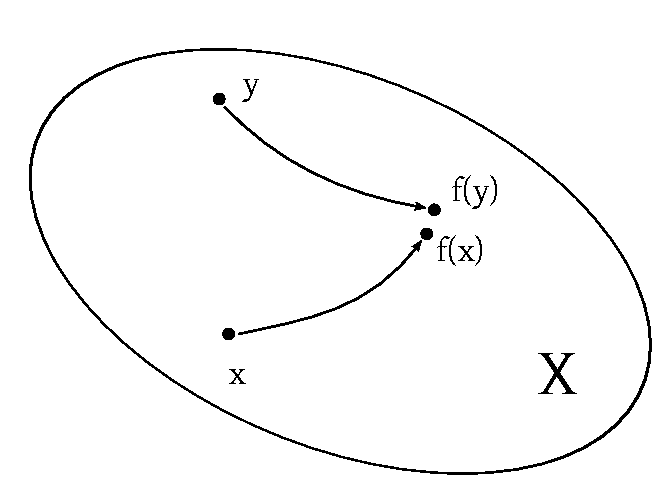
\includegraphics{img/07_contraction.pdf}
    \caption{A contraction maps to points closer to each other}
    \label{img:contraction}
  \end{center}
\end{figure}

\index{Fixed point}
\begin{theorem}[Banach fixed-point theorem] % Satz 5
  Let $f: X \to X$ be a contraction and $X$ be complete.
  Then there exists a uniquely defined $\hat{x} \in X$ such that $\hat{x} = f(\hat{x})$. $\hat{x}$ is called fixed point on $f$.
  Furthermore $x_0 \in X$ is arbitrary and $x_n = f(x_{n-1})$ for all $n \geq 1$. Compare with Figure~\ref{img:banachfixed}.
  \[ \lim_{n \to \infty} x_n = \hat{x} \]
\end{theorem}

\begin{figure}[t]
  \begin{center}
    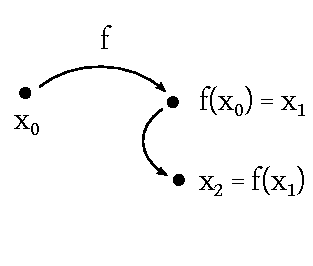
\includegraphics{img/07b_banach_fixed_point_theorem.pdf}
    \caption{Banach's Fixed Point Theorem states that applying $f$ iteratively gives a point coming closer and closer to the previous one}
    \label{img:banachfixed}
  \end{center}
\end{figure}

\begin{remark}
  The following proof is a very common exam question.
\end{remark}

\begin{proof}
  Let $x_0 \in X$ be arbitrary.
  $x_n$ is constructed inductively by $x_n = f(x_{n-1})$ for all $n \geq 1$.

  \begin{claim}
    $(x_n)_{n \in \mathbb N}$ is a Cauchy sequence in $X$.
  \end{claim}
  \begin{align*}
    d(x_n, x_{n+k}) &\leq d(x_n, x_{n+1}) + d(x_{n+1}, x_{n+2}) + \dots + d(x_{n+k-1}, x_{n+k}) \qquad \text{by triangle ineq.} \\
      &= d(x_n, x_{n+1}) + d(f(x_n), f(x_{n+1})) + \dots + d(f(x_{n+k-2}), f(x_{n+k-1})) \\
      &\leq d(x_n, x_{n+1}) + L\left(d(x_n, x_{n+1}) + d(x_{n+1}, x_{n+2}) + \dots + d(x_{n+k-2}, x_{n+k-1})\right) \\
  \intertext{this inequality is given by contraction}
      &= d(x_n, x_{n+1}) (1 + L) + L \left(d(f(x_n), f(x_{n+1})) + \dots + d(f(x_{n+k-3}), f(x_{n+k-2}))\right) \\
      &\leq d(x_n, x_{n+1}) (1 + L) + L^2 \left[d(x_n, x_{n+1} + \dots + d(x_{n + k - 3}, x_{n+k-2})\right] \\
      &\leq \dots \leq d(x_n, x_{n+1}) (1 + L + L^2 + \dots + L^{k-1}) \\
      &= d(f(x_{n-1}), f(x_n)) \left(\sum_{j=0}^{k-1} L^j\right) \leq L d(x_{n-1}, x_n) \cdot \left(\sum_{j=0}^{k-1} L^j\right) \\
      &\leq L^n d(x_0, x_1) \cdot \underbrace{\left(\sum_{j=1}^{k-1} L^j\right)}_{\leq \sum_{j=0}^\infty L^j = \frac{1}{1 - L}} \\
      &\leq \frac{L^n}{1 - L} d(x_0, x_1) \\
    d(x_n, x_{n+k}) &\leq \frac{L^n}{1 - L} d(x_0, x_1) \quad \forall n \in \mathbb N \forall k \in \mathbb N_0 \text{ with } 0 \leq L < 1
  \end{align*}
  \[ \frac{L^n}{\underbrace{1 - L}_{> 0}} d(x_0, x_1) < \varepsilon \impliedby \]
  \[ L^n < \frac{\varepsilon}{d(x_0, x_1) + 1} (1 - L) \qquad (L > 0) \]
  \[ \iff n \underbrace{\ln{L}}_{<0} < \ln \frac{\varepsilon}{d(x_0, x_1) + 1} (1 - L) \]
  \[ \iff n > \frac{1}{\ln{L}} \ln \frac{\varepsilon}{d(x_0, x_1) + 1} (1 - L) \]

  Hence $(x_n)_{n \in \mathbb N}$ is a Cauchy sequence in $X$. $X$ is complete, hence $\exists \hat{x} \in X: \hat{x} = \lim_{n \to \infty} x_n$.
  Because $\hat{x} = \lim_{n\to\infty} x_{n+1} = \lim_{n\to\infty} f(x_n) = f(\hat{x})$ where the last equality is given by continuity of $f$.
  Therefore $\hat{x} = f(\hat{x})$ is a fixed point on $f$.

  It remains to prove uniqueness:

  Let $\tilde{x} = f(\tilde{x})$. Then $d(\hat{x}, \tilde{x}) = d(f(\hat{x}), f(\tilde{x})) \leq L d(\hat{x}, \tilde{x})$ with $L < 1$.
  If $d(\hat{x}, \tilde{x}) > 0$, then $1 \leq L$. This is a contradiction.
  Hence $d(\hat{x}, \tilde{x}) = 0$ must hold, hence $\hat{x} = \tilde{x}$.
\end{proof}

\begin{remark}
  \begin{itemize}
  	\item The Fixed Point Theorem provides an algorithm for numeric computation of $\hat{x}$.
    \item It can reformulate problems $f(x) = 0$ (in $\mathbb R^n$) to
      \[ f(x) + x = g(x) = x \]
    \item Attention: The conditions of the Fixed Point Theorem cannot be changed to the structure
      \[ d(f(x), f(y)) < L \cdot d(x, y) \land L \leq 1 \]
      or
      \[ d(f(x), f(y)) \leq L \cdot d(x, y) \land L < 1 \]
      This will be discussed in the practicals.
  \end{itemize}
\end{remark}

\begin{lemma} % Lemma 7
  \label{lemma7}
  Let $X$ be a complete metric space. Let $A \subseteq X$ be closed.
  Then $(A, d)$ is itself a complete, metric space.
\end{lemma}

\begin{proof}
  Let $(x_n)_{n \in \mathbb N}$ be a Cauchy sequence in $A$ ($x_n \in A$).
  Then $(x_n)_{n \in \mathbb N}$ is also a Cauchy sequence in $X$.
  Because $X$ is complete, there exists $\hat{x} = \lim_{n\to\infty} x_n$.
  Therefore $\hat{x}$ is a contact point of $A$.
  Because $A$ is closed, $\hat{x} \in A$.

  Therefore every Cauchy sequence in $A$ has a limit point in $A$,
  hence $A$ is complete.
\end{proof}

\section{Compactness}
\subsection{Definition}

\index{Compactness}
\begin{definition} % Definition 16
  A metric space $(X, d)$ is called \emph{compact} if every sequence $(x_n)_{n \in \mathbb N}$
  has a convergent subsequence.

  Specifically, this definition is called sequence compactness. The other definition defines compactness as closed and bounded subset of an Euclidean space. The latter definition only works for a subset of branches in mathematics. Therefore the generalization is recommended to be remembered.
\end{definition}

\begin{lemma} % Lemma 8
  Let $X$ be a compact, metric space. Then $X$ is complete.
\end{lemma}
\begin{proof}
  Let $(x_n)_{n\in\mathbb N}$ be a Cauchy sequence in $X$. By compactness, it follows that
  $\exists (x_{n_k})_{k \in \mathbb N}$ with $\lim_{k\to\infty} x_{n_k} = \hat{x}$.
  Choose $\varepsilon > 0$ arbitrary and $L$ large enough such that $k \geq L \implies d(x_{n_k}, \hat{x}) < \frac\varepsilon2$. Furthermore choose $N \in \mathbb N$ large enough such that $n,m \geq N \implies d(x_n, x_m) < \frac\varepsilon2$ (satisfied, because $(x_n)_{n \in \mathbb N}$ is a Cauchy sequence).
  Choose $K \geq L$ and $n_k \geq N$. Let $n_k$ be fixed this way.
  Then it holds $\forall n \geq N: d(x_n, \hat{x}) \leq d(x_n, x_{n_k}) + d(x_{n_k}, \hat{x}) < \frac\varepsilon2 + \frac\varepsilon2 = \varepsilon$. The first summand $\frac\varepsilon2$ results from the Cauchy sequence property, the second summand $\frac\varepsilon2$ results by convergence of $(x_{n_k})$. Hence $(x_n)_{n\in\mathbb N}$ is convergent with limit $\hat{x}$.
\end{proof}

\subsection{Boundedness}
\index{Boundedness}
\begin{definition} % Definition 17
  A metric space $X$ is called \emph{bounded} if there exists $M \geq 0$, such that $d(x,y) \leq M \forall x,y \in X$.
\end{definition}
It holds for arbitrary $x \in X$ that $\forall y \in X: y \in K_M(x)$.
So, $X \subseteq K_M(x)$.
On the contrary, let $X \subseteq \overline{K_M(x)}$ and let $y \in X$ and $z \in X$ be arbitrary. Then $d(y, z) \leq d(y, x) + d(x, z) \leq M + M = 2M$. Hence, $X$ is bounded.

So, $X$ is bounded $\iff \exists x \in X \land M \geq 0: X \subseteq \overline{K_M(x)}$.

\begin{lemma} % Lemma 9
  Every compact, metric space is also bounded.
\end{lemma}

\begin{proof}
  Assume $X$ is unbounded.

  We construct a sequence of points $(x_n)_{n \in \mathbb N}$ with $d(x_n, x_m) \geq 1 \forall n,m \in \mathbb N$ with $n \neq m$.

  We use the following auxiliary result: Let $B = \bigcup_{j=1}^n K_1(z_j)$ for arbitrary $n \in \mathbb N$ and arbitrary $z_j \in X$. Then $B$ is bounded. This result will be part of the practicals.

  We construct $(x_n)_{n\in\mathbb N}$ inductively. Choose arbitrary $x_0 \in X$. Assume $(x_1, \dots, x_{n-1})$ are already found. Then,
  \[ \underbrace{X}_{\text{unbounded}} \not\subseteq \underbrace{\bigcup_{j=1}^{n-1} K_1(x_j)}_{\text{bounded}} \]
  hence $\exists x_n \in X \setminus \bigcup_{j=1}^{n-1} K_1(x_j)$.
  Because $x_n \not\in K_1(x_j)$ for $j = 0, \dots, n-1$ it is given that $d(x_n, x_j) \geq 1 \forall j < n$. We get $(x_n)_{n \in \mathbb N}$ with $d(x_n, x_m) \geq 1 \forall n \in \mathbb N \forall m < n$, hence $m \neq n$. Because $d(x_n, x_m) \geq 1$, i.e. $(x_n)_{n \in \mathbb N}$ does not contain any Cauchy sequence as subsequence, $(x_n)_{n \in \mathbb N}$ does not have a convergent subsequence. Therefore $X$ is not compact.
\end{proof}

\dateref{2018/03/15}

Every compact metric space is bounded. Every compact metric space is complete.
In $\mathbb C$ ($\mathbb R^n$), any $A \subseteq \mathbb C$ is closed.
Then $A$ with metric $d(x,y) = \card{x - y}$ is complete as metric space.

If $A$ is additionally bounded, then $A$ is compact (see course Analysis 1, Bolzano-Weierstrass).

\emph{Attention!} Let $V$ be an infinite-dimensional, complete, normed vector space.
\begin{itemize}
  \item For example, $V = \mathcal C([a,b], \mathbb R) = \setdef{f: [a,b] \to \mathbb R}{f \text{ is continuous in } [a,b]}$
  \item with norm $\norm{f}_{\infty} = \max\set{\card{f(x)}: x \in [a,b]}$
  \item and metric $\norm{f - g}_{\infty} = \max\set{\card{f(x) - g(x)}: x \in [a,b]}$
\end{itemize}
$\mathcal C([a,b], \mathbb R)$ is a complete, normed vector space.
So, $\overline{K_1(0)}$ is not compact in $\mathcal C([a,b], \mathbb R)$ (i.e. $V$, for every infinite-dimensional vector space).

\emph{Again:} do not remember \enquote{compactness} as closed and bounded, because this definition only holds in the finite-dimensional case.

In the last proof, we have shown: If a sequence $(x_n)_{n \in \mathbb N}$ with $x_n \in X$ and $d(x_n, x_m) \geq 1$ (or $\geq \varepsilon$) $\forall n \neq m \implies X$ is not compact.

\subsection{Total boundedness}

\index{Total boundedness}
\begin{definition}
  $X$ is called totally bounded, if for every $\varepsilon > 0$, finitely many points $X_1^\varepsilon$, $X_2^\varepsilon$, \dots, $X_{N(\varepsilon)}^\varepsilon$ such that $X \subseteq \bigcup_{i=1}^{N(\varepsilon)} K_{\varepsilon}(X_i^\varepsilon)$.

  Hence, for every $x \in X$, there exists some $X_j^\varepsilon$ such that $d(X, X_j^\varepsilon) < \varepsilon$.
\end{definition}

\begin{remark}[For the practicals]
  Let $X$ be totally bounded, then there does not exist some sequence $(x_n)_{n \in \mathbb N}$ with $d(x_n, x_m) \geq \varepsilon \forall n \neq m$. It holds, that $X$ is compact if and only if $X$ is totally bounded and complete.
\end{remark}

\subsection{Compactness, continuity and openness}
\begin{theorem} % Satz 6
  \label{satz6}
  Let $f: X \to Y$ be continuous. Let $X$ be compact. Then image $f(X) \subseteq Y$ is also compact.
\end{theorem}

Be aware, that this proof is a common exam question and students often begin with the wrong order.

\begin{proof}
  Let $(y_n)_{n \in \mathbb N}$ be an arbitrary sequence in $f(X)$. Show that $(y_n)_{n\in\mathbb N}$ has a convergent subsequence.
  Because $y_n \in f(X)$, there exists at least one $x_n$ with $y_n = f(x_n)$.
  Then $(x_n)_{n \in \mathbb N}$ is a sequence in $X$, $X$ is compact, hence there exists a subsequence $(x_{n_k})_{k \in \mathbb N}$ with $\lim_{k\to\infty} x_{n_k} = \hat{x} \in X$. Because $f$ is continuous, $\lim_{k\to\infty} f(x_{n_k}) = \lim_{k\to\infty} y_{n_k} = f(\hat{x}) \eqqcolon \hat{y}$.
  So $(y_n)_{n\in\mathbb N}$ has a convergent subsequence. Hence $f(X) \subseteq Y$ is compact.
\end{proof}

\begin{theorem}[Conclusion] % Satz 7
  \label{satz7}
  Let $X$ be compact, $f: X \to \mathbb R$ continuous on $X$.
  Then there exists $\underline{x}$ and $\overline{x} \in X$, such that
  \[ f(\underline{x}) \leq f(x) \leq f(\overline{x}) \qquad \forall x \in X \]
  Hence, $f$ has a maximum and a minimum.
\end{theorem}

\begin{proof}
  $f(X) \subseteq \mathbb R$ is compact (Theorem~\ref{satz6}), hence $f(X)$ is bounded and complete, hence closed in $\mathbb R$.
  There exists $\xi \in \mathbb R$ with $\xi = \sup{f(X)}$, because $f(X)$ is complete and $\xi$ is a contact point of $f(X)$, so $\xi \in f(X)$, hence $\exists \overline{x} \in X: \xi = f(\overline{x})$. Furthermore, $\xi$ is an upper bound of $f(X) \to f(x) \leq \xi = f(\overline{x}) \forall x \in X$.

  For $\underline{x}$, it works the same way.
\end{proof}

\begin{theorem} % Satz 8
  \label{satz8}
  Let $f: X \to Y$ be continuous on $X$ and $X$ is compact. Then $f$ is uniformly continuous on $X$.
\end{theorem}

\begin{proof}[Indirect proof]
  Assume $X$ is compact, $f: X \to Y$ is continuous, but not uniformly continuous. Uniform continuity:
  \[ \forall \varepsilon > 0 \exists \delta > 0: \forall x, y \in X: d_X(x,y) < \delta \implies d_Y(f(x), f(y)) < \varepsilon \]
  Not uniformly continuous:
  \[ \exists \varepsilon > 0 \forall \delta_n = \frac1n (n \in \mathbb N) \exists x_n, y_n \in X: d_X(x_n, y_n) < \frac1n \land d_Y(f(x_n), f(y_n)) \geq \varepsilon \]
  Now choose some $(x_n)$ and $(y_n)$. We will use a specific $\varepsilon$ later.
  Because $X$ is compact, there exists a convergent subsequence of $(x_n)_{n \in \mathbb N}$, hence $\lim_{k\to\infty} x_{n_k} = \hat{x}$.
  The sequence $(y_{n_k})_{k \in \mathbb N}$ has a convergent subsequence itself:
  \[ \lim_{l\to\infty} y_{(n_k)_l} = \hat{y} \]
  Because $(x_{n_k})_{n \in \mathbb N}$ is convergent, the subsequence $(x_{(n_k)_l})_{l \in \mathbb N}$ converges towards the same limit $\hat{x}$.
  \[ \tilde{x}_l \coloneqq x_{n_{k_l}} \qquad \tilde{y}_l \coloneqq y_{n_{k_l}} \]
  because $l \leq x_{n_l}$ and
  \[ d_X(\tilde{x}_l, \tilde{y}_l) = d_X(x_{n_{k_l}}, y_{n_{k_l}}) \underbrace{<}_{\text{by assumption}} \frac{1}{n_{k_l}} \leq \frac1l \]

  \begin{claim}
    For $\hat{x} = \lim_{l\to\infty} \tilde{x}_l$ and $\hat{y} = \lim_{l\to\infty} \tilde{y}_l$, it holds that $\hat{x} = \hat{y}$.
  \end{claim}
  \begin{proof}
    Let $\varepsilon' > 0$ be arbitrary, $l$ large enough such that
    \begin{itemize}
      \item $\frac1l < \frac{\varepsilon'}{3}$
      \item $d_X(\tilde{x}_l, \hat{x}) < \frac{\varepsilon'}{3}$
      \item $d_X(\tilde{y}_l, \hat{y}) < \frac{\varepsilon'}{3}$
    \end{itemize}
    Therefore
    \[
      d_X(\hat x, \hat y) \leq d_X(\hat x, \tilde x_l) + d_X(\tilde x_l, \tilde y_l) + d_X(\tilde y_l, \hat y)
      < \frac{\varepsilon'}{3} + \frac1l + \frac{\varepsilon'}{3} < \varepsilon'
    \]
    Therefore $d_X(\hat{x}, \hat{y}) = 0$, hence $\hat{x} = \hat{y}$.
  \end{proof}
  Because $f$ is continuous and $\tilde{x_l} \to \hat{x}$ and $\tilde{y}_l \to \hat{x}$, there exists $l \in \mathbb N$ such that
  \[ d_Y(f(\tilde x_l), f(\hat{x})) < \frac\varepsilon2 \]
  and also
  \[ d_Y(f(\tilde y_l), f(\hat{x})) < \frac\varepsilon2 \]
  where $\varepsilon$ is the epsilon from the very beginning of the proof.

  \[ \implies d_Y(f(\tilde x_l), f(\hat{x})) + d_Y(f(\tilde y_l), f(\hat{x})) < \varepsilon \]
  This contradicts to
  \[ d_Y(f(\tilde{x}_l), f(\tilde{y}_l)) = d_Y(f(x_{n_{k_l}}), f(y_{n_{k_l}})) \geq \varepsilon \]

  Hence, $f$ is uniformly continuous.
\end{proof}

Subsets of $(\mathbb R^n, \norm{\cdot})$ (or $(V, \norm{\cdot})$) as metric spaces.

We consider $\Omega \subseteq V$ where $V$ is a normed vector space.
$(\Omega, d)$ is $d(x, y) = \norm{x - y}$ is a metric space.
\[ K_r^\Omega(x) = \setdef{y \in \Omega}{\norm{y - x} < r} \]
is a sphere with center $x$ and radius $r$ in $\Omega$.
\[ K_r^V(x) = \setdef{y \in V}{\norm{y - x} < r} \]
obvious: $K_r^\Omega(x) = \Omega \cap K_r^V(x)$.

\begin{figure}[t]
  \begin{center}
    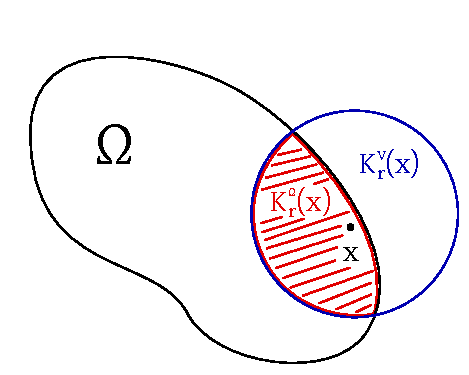
\includegraphics{img/08.pdf}
    \caption{Subsets of $(\mathbb R^n, \norm{\cdot})$ as metric spaces}
    \label{img:subs}
  \end{center}
\end{figure}

\begin{lemma} % Lemma 10
  Let $O' \subseteq \Omega \subseteq V$.

  Then $O'$ is open in $\Omega \iff$ there exists $O \subseteq V$ is open in $V$ such that $O' = O \cap \Omega$.
\end{lemma}

\begin{proof}
  \begin{description}
    \item[$\Rightarrow$]
      Let $O' \subseteq \Omega$ be open in $\Omega$ and $x \in O'$ be arbitrary.
      Then there exists $r(x) > 0: x \in K_{r(x)}^\Omega(x) = K_{r(x)}^V(x) \cap \Omega \subseteq O'$.
      Then
      \[
        O' = \bigcup_{x \in O'} = \set{x} \subseteq \bigcup_{x \in O'} K_{r(x)}^\Omega(x)
        = \left(\bigcup_{x \in O'} (K_{r(x)}^V(x)\right) \cap \Omega)
        = \underbrace{\left(\bigcup_{x \in O'} K_{r(x)}^V(x)\right)}_{= O \subseteq V \text{ is open in } V} \cap \Omega
        \subseteq O'
      \]
      So every $\subseteq$ in this inclusion chain is actually an equality. So $O' = O \cap \Omega$.

    \item[$\Leftarrow$]
      Let $O' = O \cap \Omega$ and $x \in O'$ be chosen arbitrarily.
      Because $x \in O$ and $O$ is open in $V$.
      \[ \exists r > 0: K_r^V(x) \subseteq O \implies \underbrace{K_r^V(x) \cap \Omega}_{= K_r^\Omega(x)} \subseteq O \cap \Omega = O' \]
      So $O'$ is open in $\Omega$.
  \end{description}
\end{proof}

\begin{remark}
  $A' \subseteq \Omega$ is closed in $\Omega \iff \exists A \subseteq V$ closed in $V$ with $A' = A \cap \Omega$.
\end{remark}

\index{Relative topology}
\index{Trace topology}
\index{Subspace topology}
\begin{remark}
  Let $T$ be an arbitrary topological space with topology $\tau$ on $T$ (a system of open sets).
  Furthermore let $\Omega \subseteq T$.

  Then $\Omega$ itself is a topological space with $O' \subseteq \Omega$ is open $\iff \exists O \subset T$ open in $T$ with $O' = O \cap \Omega$.

  Also called \enquote{subspace topology}, \enquote{trace topology} or \enquote{relative topology}.
\end{remark}

Attention!
\[ O' \subseteq \Omega \text{ open in } \Omega \implies O' \text{ open in } V \]
does \emph{not} hold in general.

\begin{example}
  \[ \Omega = [0,1] \cap [0,1) \]
  $K_{\frac12}(p) \cap \Omega$ is open in $\Omega$ but not open in $\mathbb R^2$.
\end{example}

Analogously,
\[ A' \subseteq \Omega \text{ is closed} \implies A' \text{ closed in } V \]
does \emph{not} hold in general.

\begin{remark}
  $K$ is compact in $\Omega \implies K$ is compact in $V$
\end{remark}

Let $(x_n)_{n \in \mathbb N}$ be a sequence in $K$.
Compactness $\implies \exists (x_{n_k})_{k \in \mathbb N}: x_{n_k} \to \hat{x}$ for $k \to \infty$ and $K \subseteq \Omega \subseteq V$.

Then $(x_n)_{n \in \mathbb N}$ also has a convergent subsequence in $V$.

\subsection{Normed vector spaces}

\begin{definition} % Definition 19
  Let $V$ be a vector space and $\norm{\cdot}_1$ and $\norm{\cdot}_2$ are normed on $V$.
  We say, $\norm{\cdot}_1$ is equivalent to norm $\norm{\cdot}_2$, if $0 < m \leq M$ exist such that
  \[ m \norm{v}_1 \leq \norm{v}_2 \leq M \norm{v}_1 \forall v \in V \]
\end{definition}

\begin{remark}
  Equivalence of norms is an equivalence relation.
  \begin{description}
    \item[reflexivity]
      $\norm{\cdot}_1$ is equivalent to $\norm{\cdot}_1$ with $m = M = 1$.
    \item[symmetry]
      \[ m \norm{v}_1 \leq \norm{v}_2 \implies \norm{v}_1 \leq \frac1m \norm{v}_2 \land \norm{v}_2 \leq M \cdot \norm{v}_1 \implies \frac1M \norm{v}_2 \leq \norm{v}_1 \]
      \[ \implies \underbrace{\frac1M}_{m'} \norm{v}_2 \leq \norm{v_1} \leq \underbrace{\frac1m}_{M'} \norm{v}_2 \]
      hence the equivalence relations of norms are symmetrical.
    \item[transitivity]
      Let $\norm{\cdot}_1$ and $\norm{\cdot}_2$ be equivalent.
      Let $\norm{\cdot}_2$ and $\norm{\cdot}_3$ be equivalent.

      \[ m \cdot \norm{v}_1 \leq \norm{v}_2 \leq M \norm{v}_1 \forall v \in V \]
      \[ m' \cdot \norm{v}_2 \leq \norm{v}_3 \leq M' \norm{v}_2 \forall v \in V \]
      \[ \implies m \cdot m' \norm{v}_1 \leq m' \norm{v}_2 \leq \norm{v}_3 \leq M' \norm{v}_2 \leq M \cdot M' \norm{v}_1 \]
  \end{description}
\end{remark}

\dateref{2018/03/20}

Addendum:
\begin{itemize}
  \item Let $(x_n)_{n \in \mathbb N}$ be in $(X, d)$, then
    \[ \underbrace{x = \lim_{n\to\infty} x_n}_{\text{in } X} \iff \underbrace{\lim_{n\to\infty} d(x_n, x) = 0}_{\text{in } \mathbb R} \]
    \[ (\iff \lim_{n\to\infty} \norm{x_n - x} = 0 \text{ in normed vector spaces } V) \]
  \item Reversed triangle inequality: Let $V$ be a normed vector space. Let $x, y \in V$.
    \[ \norm{x} = \norm{x - y + y} \leq \norm{x - y} + \norm{y} \]
    Hence,
    \[ \norm{x} - \norm{y} \leq \norm{x - y} \]
    By exchanging $x$ and $y$,
    \[ \norm{y} - \norm{x} \leq \norm{x - y} \]
    \[ \implies \card{\norm x - \norm y} \leq \norm{x - y} \]
  \item Define the map $n: V \to [0, \infty)$ on $(V, \norm{\cdot})$ with $n(x) = \norm{x}$.
    Then $n$ is continuous on $V$ because
    \[ \card{n(x_1) - n(x_2)} = \card{\norm{x_1} - \norm{x_2}} \leq \norm{x_1 - x_2} \]
    Hence, $n$ is Lipschitz continuous with constant $1$.
\end{itemize}

Regarding the equivalence of norms:

\begin{lemma} % Lemma 11
  Let $\norm{\cdot}_1$ and $\norm{\cdot}_2$ be equivalent norms on $V$. Then,
  \begin{enumerate}
    \item $\lim_{n\to\infty} \norm{x_n - x}_1 = 0 \iff \lim_{n\to\infty} \norm{x_n - x}_2 = 0$,
      hence $(x_n)_{n\in\mathbb N}$ is convergent with limit $x$ in regards of $\norm{\cdot}_1$
      $\iff$ $(x_n)_{n\in\mathbb N}$ is convergent with limit $x$ in regards of $\norm{\cdot}_2$.
    \item $O \subseteq V$ is open in regards of $\norm{\cdot}_1 \iff O$ is open in regards of $\norm{\cdot}_2$,
      hence $\tau_1 = \tau_2$ (topologies are equivalent).
    \item $K \subseteq V$ is compact in regards of $\norm{\cdot}_1 \iff K$ is compact in regards of $\norm{\cdot}_2$.
  \end{enumerate}
\end{lemma}

\begin{proof}
  Let $\norm{\cdot}_1$ and $\norm{\cdot}_2$ are equivalent, hence $\exists m, M > 0: m \norm{x}_1 \leq \norm{x}_2 \leq M \norm{x}_1 \forall x \in V$.
  \begin{enumerate}
    \item Let $\varepsilon > 0$ and $\lim_{n\to\infty} \norm{x_n - x}_1 = 0$.
      Choose $N \in \mathbb N$ such that $n \geq N \implies \norm{x_n - x}_1 < \frac{\varepsilon}{M}$. For those $n$,
      \[ \norm{x_n - x}_2 \leq M \norm{x_n - x}_1 < \frac{\varepsilon}{M} \cdot M = \varepsilon \]
      Hence, $\lim_{n\to\infty} \norm{x_n - x}_2 = 0$.
    \item $K_r^2(x) = \setdef{y \in V}{\norm{y - x}_2 < r}$. For $y \in K_r^2(x)$,
      \[ m \norm{y - x}_1 \leq \norm{y - x}_2 < r \]
      hence,
      \[ \norm{y - x}_1 < \frac rm \implies y \in K_{\frac rm}^1(x) \]
      hence $K_r^2(x) \subseteq K_{\frac rm}^1(x)$.
      Let $y \in K_{\frac rM}^1(x)$. Then,
      \[ \norm{y - x}_2 \leq M \norm{y - x}_1 < M \cdot \frac rM = r \]
      hence $y \in K_r^2(x)$. $\implies K_{\frac rM}^1(x) \subseteq K_r^2(x)$.
      Now let $O$ be open in regards of $\norm{\cdot}_2$, hence
      \[ \forall x \in O \exists r > 0: K_r^2(x) \subseteq O \implies K_{\frac rM}^1(x) \subseteq K_r^2(x) \subseteq O \]
      so $O$ is open in regards of $\norm{\cdot}_1 \implies O$ is open in regards of $\norm{\cdot}_2$ analogously.
    \item
      Let $K$ be compact in regards of $\norm{\cdot}_1$ and $(x_n)_{n \in \mathbb N}$ be a sequence in $K$.
      Then there exists a subsequence $(x_{n_k})_{k \in \mathbb N}$ with $\norm{x_{n_k} - x}_1 \to 0$ for $k \to \infty$
      $\xRightarrow{\text{by the first property}} \norm{x_{n_k} - x}_2 \to 0$. Hence $(x_{n_k})_{k \in \mathbb N}$ is also a convergent subsequence in regards of $\norm{\cdot}_2$.
  \end{enumerate}
\end{proof}

\begin{remark}[Proven in the practicals]
  Let $(x_n)_{n\in\mathbb N}$ be a sequence in $\mathbb R^k$
  \[ \norm{x}_{\infty} = \max\setdef{\card{x^i}}{i = 1, \dots, n} \]
  \[ x = \begin{bmatrix} x^1 \\ x^2 \\ \vdots \\ x^k \end{bmatrix} \]
  Then $\lim_{n\to\infty} \norm{x_n - x}_{\infty} = 0 \iff \lim_{n\to\infty} \card{x_n^i - x^i} = 0$ for all $i \in \set{1, \dots, k}$.
\end{remark}

\begin{theorem}[Bolzano-Weierstrass theorem in $\mathbb R^k$]
  Let $K \subseteq \mathbb R^k$ be closed and bounded.
  Then $K$ is compact in $(\mathbb R^k, \norm{\cdot}_{\infty})$.
\end{theorem}

\begin{proof}
  Let $\norm{x}_{\infty} \leq M \forall x \in K \iff \card{x^i} \leq M \forall x \in K$ and $i \in \set{1, \dots, k}$.
  Choose $(x_n)_{n \in \mathbb N}$ an arbitrary sequence in $K$ $(x_n^i)_{n \in \mathbb N}$ is a bounded sequence in $\mathbb R$.
  Because $(x_n^1)_{n \in \mathbb N}$ is bounded, there exists a convergent subsequence $\left(x_{n_{l_1}}^1\right)_{l_1 \in \mathbb N}$
  \[ \lim_{l_1 \to \infty} x_{n_{l_1}}^1 = x^1 \]
  Consider $(x_{n_{l_1}}^2)_{l_1 \in \mathbb N}$, a subsequence of a bounded sequence, hence bounded itself.
  By the Bolzano-Weierstrass theorem in $\mathbb R$, there exists a convergent subsequence $(x_{n_{{l_1}_{l_2}}}^2)_{l_2 \in \mathbb N}$ with $\lim_{l_2 \to \infty} x_{n_{{l_1}_{l_2}}}^2 = x^2$.
  Consider $x_{n_{{l_1}_{l_2}}}^1$ as subsequence of $x_{n_{l_1}}^1$ is already convergent, hence $\lim_{l_2 \to \infty} x_{n_{{l_1}_{l_2}}}^1 = x^1$. Furthermore, for indices up to $i$:
  \[ \lim_{l_k \to \infty} x_{n_{{{{l_1}_{l_2}}_{\ldots}}_{l_k}}} = x^i \qquad \text{ for } i = 1, \dots, k \]
  Hence, with $\tilde{x_{l_k}} = x_{n_{{{{l_1}_{l_2}}_{\ldots}}_{l_k}}}$ gives a subsequence of $x_n$, converging by each coordinate. Thus,
  \[ \lim_{l_k \to \infty} \norm{\tilde{x}_{l_k} - x}_{\infty} = 0 \]
  Because $\tilde{x}_{l_n} \in K$ and $K$ is closed, $x \in K$.
  Hence $K$ is compact.
\end{proof}

\begin{theorem}[Norm equivalence in $\mathbb R^k$] % Satz 10
  In $\mathbb R^k$, all norms are equivalent.
\end{theorem}

\begin{proof}
  We show: Let $\norm{\cdot}$ be an arbitrary norm on $\mathbb R^n$. Then $\norm{\cdot}$ is equivalent to $\norm{\cdot}_{\infty}$. By transitivity of norm equivalence, two arbitrary norms are equivalent to each other.
  \begin{enumerate}
    \item Let $(e_1, e_2, \dots, e_k)$ be the canonical basis in $\mathbb R^k$.
      \[ x = \begin{bmatrix} x^1 \\ \vdots \\ x^k \end{bmatrix} = \sum_{j=1}^k x^j e_j \]
      Furthermore let $M' = \max\set{\norm{e_j}: j = 1, \dots, k}$ with $\norm{e_j} \neq 0$ and $M' > 0$.
      Then
      \begin{align*}
        \norm{x} &= \norm{\sum_{j=1}^k x^j e_j} \leq \sum_{j=1}^k \norm{x^j e_j} = \sum_{j=1}^k \card{x^j} \norm{e_j} \\
                 &\leq M' \sum_{j=1}^k \underbrace{\card{x_j}}_{\leq \norm{x}_\infty} \leq \underbrace{M' \cdot k}_{M} \norm{x}_{\infty} = M \norm{x}_\infty
      \end{align*}
    \item
      We consider $\nu: \mathbb R^k \to [0, \infty)$.
      $\nu(x) = \norm{x}$ as map on $(\mathbb R^k, \norm{\cdot}_{\infty})$.

      \begin{claim}
        $\nu$ is continuous on $(\mathbb R^k, \norm{\cdot}_{\infty})$.
      \end{claim}
      \begin{proof}
        Show that,
        \[ \card{\nu(x) - \nu(y)} = \card{\norm{x} - \norm{y}} \underbrace{\leq}_{\text{reversed triangle ineq.}} \norm{x - y} \underbrace{\leq}_{\text{because of (1)}} M \norm{x - y} \]
        Hence $\nu$ is Lipschitz continuous.
      \end{proof}

      We consider $S_{\infty}^{k-1} = \set{x \in \mathbb R^k}{\norm{x}_{\infty} = 1} = \operatorname{boundary}(K_1^\infty(0)$.
      $S_{\infty}^{k-1}$ is bounded.

      Let $(x_n)_{n \in \mathbb N}$ be a sequence in $S_{\infty}^{k-1}$ with $x = \lim_{n\to\infty} x_n$. Because $n(x) = \norm{x}_{\infty}$ is continuous,
      \[ \lim_{n\to\infty} \underbrace{\norm{x_n}_{\infty}}_{=1} = \underbrace{\norm{x}}_{=1} \]
      Hence $x \in S_{\infty}^{k-1}$. Hence, $S_{\infty}^{k-1}$ is closed in $(\mathbb R^k, \norm{\cdot}_{\infty})$.
      Hence $S_{\infty}^{k-1}$ is compact in $(\mathbb R^k, \norm{\cdot}_{\infty})$, $\nu: S_{\infty}^{k-1} \to [0, \infty)$, with $S_{\infty}^{k-1}$ compact, is continuous.
      Has a minimum $n$ on $S_{\infty}^{k-1}$. Thus there exists $\overline{x} \in S_{\infty}^{k-1}: \underbrace{m}_{> 0} = \norm{\underbrace{\overline{x}}_{\neq 0}} \leq \norm{x} \forall x \in S_{\infty}^{-1}$.
      Let $x \in \mathbb R^k$ be arbitrary with $x \neq 0$. Then, $\frac{x}{\norm{x}_{\infty}} \in S_{\infty}^{k-1}$ and
      \[ m \leq \norm{\frac{x}{\norm{x}_{\infty}}} = \frac{1}{\norm{x_{\infty}}} \norm{x} \implies m \norm{x}_{\infty} \leq \norm{x} \]
      Inequality also holds true for $x = 0$.
  \end{enumerate}
\end{proof}

\section{Integration calculus}
\subsection{Partitions and refinements}

\index{Partition of an interval}
\index{Step function}
\begin{definition}
  Let $a < b$ with $a, b \in \mathbb R$. We consider functions of $[a,b]$.
  We call $(x_j)_{j = 0}^n$ a \emph{partition of $[a,b]$} if $a = x_0 < x_1 < x_2 < \dots < x_n = b$.
  $x_j$ decomposes $[a,b]$ in subintervals $(x_{j-1}, x_j)$.
  $\varphi: [a,b] \to \mathbb R$ is called \emph{step function} in $[a,b]$ in regards of partition $(x_j)_{j=0}^n$
  if $\varphi|_{(x_{j-1}, x_j)} = c_j$, so constant for $j=1,\dots,n$.

  \begin{figure}
    \begin{center}
      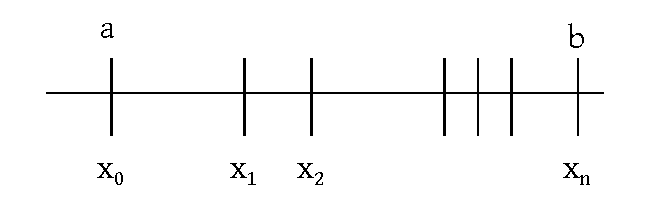
\includegraphics{img/09_subintervals.pdf}
      \caption{Illustration of a partition}
      \label{img:subintervals}
    \end{center}
  \end{figure}

  $\varphi$ is called \emph{step function} in $[a,b]$ if there exists a partition such that $\varphi$ is a subsequence.
  \[ \tau[a,b] = \set{\varphi: [a,b] \to \mathbb R: \varphi \text{ is subsequence}} \]

  Let $(\xi_i)_{i=0}^m$ be a partition of $[a,b]$ and $(x_j)_{j=0}^n$ is a partition as well.
  Then we call $(\xi_i)_{i=0}^m$ a \emph{refinement} of $[a,b]$ and $(x_j)_{j=1}^n$ as well.
  Then $(\xi_i)_{i=0}^n$ is a refinement of $(x_j)_{j=0}^k$ if
  $\set{x_0, x_1, \dots, x_n} \subseteq \set{\xi_0, \xi_1, \dots, \xi_m}$

  \begin{figure}[h]
    \begin{center}
      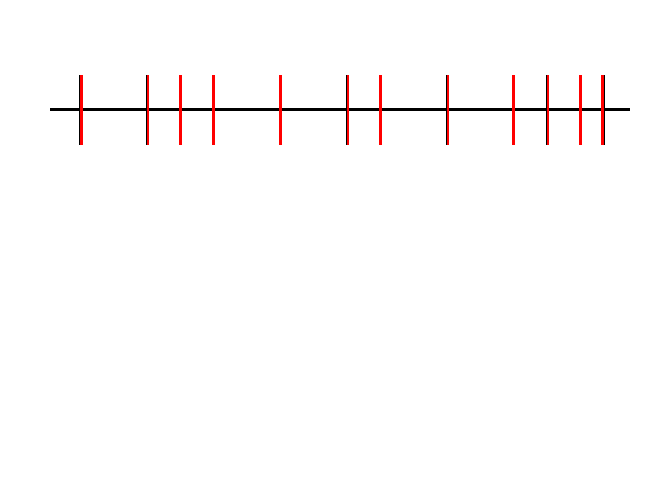
\includegraphics{img/10_refinement.pdf}
      \caption{(top) Refinement (middle) function values in points $x_j$ are unrestricted (bottom) step functions on a refinement}
      \label{img:refine}
    \end{center}
  \end{figure}

  Compare with Figure~\ref{img:refine}.
  Functions values in boundaries $x_{j-1}$ and $x_j$ do not have any constraints and will be relevant for an integral.
  A $\varphi$ can be a step function in terms of many, various partitions.
\end{definition}

\begin{lemma}
  Let $\varphi \in \tau[a,b]$ be a step function in terms of partition $(x_j)_{j=0}^n$
  and let $(\xi_i)_{i=0}^m$ be a refinement of $(x_j)_{j=0}^n$.
  Then $\varphi$ is also a step function in terms of $(\xi_i)_{i=0}^m$.
\end{lemma}

\begin{proof}
  Refinement: For every $j \in \set{0,\dots,n}$ there exists $i_j \in \set{0,\dots,m}$ such that $X_j = \xi_{i_j}$.
  $i_0 = 0, i_n = m$. $i_{j-1} < i_j$.

  Let $i \in \set{1, \dots, m}$. Then there exists a uniquely determined $j \in \set{1, \dots, n}$ such that $\xi_{i_{j-1}} < \xi_i \leq \xi_j$
  Compare with Figure~\ref{img:xi}.

  \begin{figure}[t]
    \begin{center}
      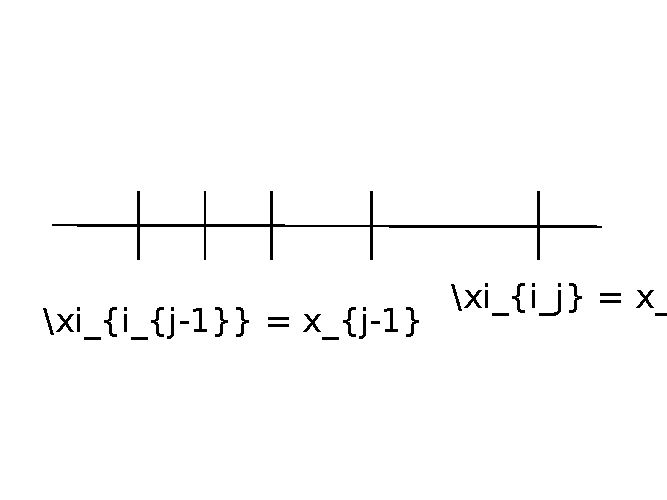
\includegraphics{img/11_xi.pdf}
      \caption{$\xi$ on a refinement $x_{i_j}$}
      \label{img:xi}
    \end{center}
  \end{figure}

  Then $(\xi_{i-1}, \xi_i) \subseteq \underbrace{(\xi_{i_{j-1}})}_{= (x_{j-1}, x_j)}, \xi_{i_j})$ and $\varphi|_{(\xi_{i-1}, \xi_j)} = c_j = \text{const}$. So $\varphi$ is a subsequence in regards of $(\xi_i)_{i=0}^m$.
\end{proof}

\begin{definition}
  Let $\varphi \in \tau[a,b]$ in terms of partition $(X_j)_{j=0}^n$ with $\varphi|_{(X_{j-1}, X_j)} = c_j$ and $\triangle X_j = X_j - X_{j-1} > 0$ for $g = 1,\dots,n$. Then we define \dots
  \[ \int_a^b \varphi \, dx = \sum_{j=1}^n c_j \triangle x_j \]
  is called \emph{integral of $\varphi$} in terms of partition $(x_j)_{j=0}^n$
\end{definition}

\dateref{2018/03/22}

Step function $\varphi$. $\varphi|_{x_{j-1},x_j} = c_j$
\[ \Delta x_j \coloneqq x_j - x_{j-1} \]
\[ \int_a^b \varphi \, dx = \sum_{j=1}^n c_j \cdot \Delta x_j \]

\begin{figure}[!h]
  \begin{center}
    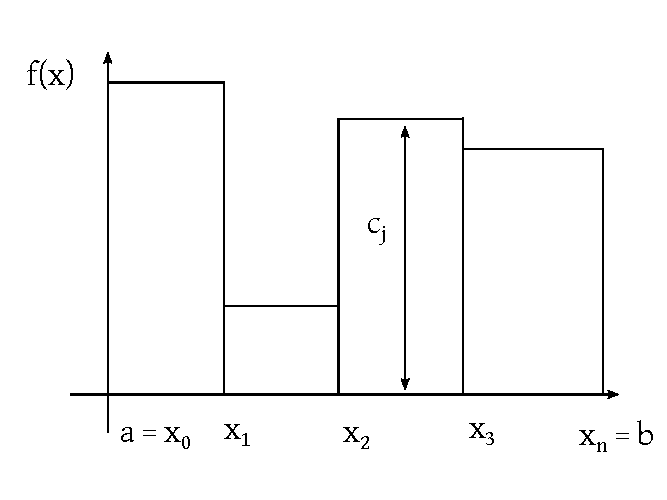
\includegraphics{img/12_integral_of_a_step_function.pdf} % TODO: too large
    \caption{Integral of a step function as sum of areas of rectangles}
  \end{center}
\end{figure}

\begin{lemma} % Lemma 2
  \label{lemma2}
  Let $(x_i)_{j=0}^n$ be a partition of $[a,b]$ and $(\xi_i)_{i=0}^m$ be a refinement of $(x_j)_{j=0}^n$.
  Furthermore let $\varphi$ be a subsequence with respect to $(x_j)_{j=0}^n$ (so also with respect to $(\xi_j)_{i=0}^m$).
  Then the integrals of $\varphi$ with respect to $(x_j)_{j=0}^n$ and $(\xi_i)_{i=0}^m$ are equal.
\end{lemma}

\begin{proof}
  There exist indices $i_j$ for $j=0$, $n$ such that $x_j = \xi_{ij}$.
  \[ i_0 = 0 \qquad i_n = m \qquad i_{j-1} < i_j \]
  \[ \Delta x_j = x_j - x_{j-1} = \xi_{i_j} - \xi_{i_{j-1}} = \xi_{i_j} - \xi_{i_{j-1}} = \underbrace{\sum_{i=i_{j-1}+1}^{i_j}}_{\text{telescoping sum}} (\xi_i - \xi_{i-1}) = \sum_{i=i_{j-1}+1}^{i_j} \Delta \xi_i \]
  \[ \varphi|_{x_{j-1},x_j} = c_j \implies \varphi|_{(\xi_{i-1},\xi_i)} = c_j \text{ for } i = i_{j-1}+1, \dots, i_j \]
  \[ \tilde{c_i} = \varphi|_{(\xi_{i-1},\xi_i)} \]
  \[ \underbrace{\sum_{i=1}^m \tilde{c_i} \Delta \xi_i}_{\text{integral of $\varphi$ w.r.t $(\xi_i)_{i=0}^m$}} = \sum_{j=1}^n \sum_{i=i_{j-1}+1}^{i_j} \tilde{c_i} \Delta \xi_i = \sum_{j=1}^n c_j \underbrace{\sum_{i=i_{j-1}+1}^{i_j} \Delta \xi_i}_{= \Delta x_j} = \sum_{j=1}^n c_j \Delta x_j \]
  This is the integral of $\varphi$ with respect to $(x_j)_{j=0}^n$.
\end{proof}

\begin{lemma} % Lemma 3
  \label{lemma3}
  Let $\varphi$ be a step function with respect to $(x_j)_{j=0}^n$ and $(w_i)_{i=0}^L$.
  Then the integrals of $\varphi$ with respect to $(x_j)_{j=0}^n$ and with respect to $(w_l)_{l=0}^L$ equal.
\end{lemma}

\begin{proof}
  Let $\setdef{\xi_i}{i = 1, \dots, m} = \setdef{x_j}{j = 0, \dots, n} \cup \setdef{w_l}{l = 0, \dots, L}$
  with $\xi_0 = a$, $\xi_m = x_n = w_L = b$ and $\xi_{i-1} < \xi_i$ for $i = 1, \dots, m$.
  Then $(\xi_i)_{i=0}^m$ is a refinement of $(x_j)_{j=0}^n$ as well as $(w_l)_{l=0}^L$.
  By Lemma~\ref{lemma2}, the integral of $\varphi$ with respect to $(x_j)_{j=0}^n =$ integral of $\varphi$
  with respect to $(\xi_i)_{i=1}^m =$ integral of $\varphi$ with respect to $(w_l)_{l=0}^L$.
  Here we discard the statement \enquote{with respect to $(x_j)_{j=0}^n$}.
\end{proof}

\begin{lemma} % Lemma 4
  \label{lem4}
  Let $f,g$ be step functions on $[a,b]$. $f,g \in \tau[a,b]$.
  \begin{itemize}
    \item
      for $\alpha, \beta \in \mathbb R$, let $\alpha f + \beta g \in \tau[a,b]$ and
      \[ \int_a^b (\alpha f + \beta g) \, dx = \alpha \int_a^bf \, dx + \beta \int_a^b g \, dx \]
      Hence, the integral is linear on $[a,b]$. $\tau[a,b]$ is a vector space.
    \item $f \leq g$ in $[a,b]$, then $\int_a^b f \, dx \leq \int_a^b g \, dx$ (monotonicity).
    \item $\card{\int_a^b f \, dx} \leq \int_a^b \card{f} \, dx$ ($\card{f(x)}$ is also a step function)
  \end{itemize}
\end{lemma}

\begin{proof}
  \begin{enumerate}
    \item
      Let $f,g \in \tau[a,b]$. Let $(\xi_i)_{i=0}^m$ be a partition such that
      $f|_{(\xi_{i-1},\xi_i)} = c_i$ and $g|_{(\xi_{i-1},\xi_i)} = d_i$.
      Then
      \begin{align*}
        \int_a^b (\alpha f + \beta g) \, dx
          &= \sum_{i=1}^m (\alpha c_i + \beta d_i) \delta \xi_i \\
          &= \alpha \sum_{i=1}^m c_i \delta \xi_i + \beta \sum_{i=1}^m d_i \delta \xi_i
          = \alpha \int_a^b f \, dx + \beta \int_a^b g \, dx
      \end{align*}
      Furthermore,
      \[ (\alpha f + \beta g)|_{(\xi_{i-1},\xi_i)} = \alpha c_i + \beta d_i = \text{ const.} \]
      Thus,
      \[ \alpha f + \beta g \in \tau[a,b] \]
    \item
      Let $h \in \tau[a,b]$ and $h(x) \geq 0 \forall x \in [a,b]$,
      then $v_i = h|_{(\xi_{i-1}, \xi_i)} \geq 0$ and
      \[ \int_a^b h \, dx = \sum_{i=1}^m \underbrace{h_i}_{\geq 0} \underbrace{\triangle \xi_i}_{\geq 0} \geq 0 \]
      Now let $f, g \in \tau[a,b]$; $f \leq g$. Then $h = g - f \in \tau[a,b]$ (membership because of (1.)) and $h \geq 0$.
      Therefore,
      \[ 0 \leq \int_a^b h \, dx = \int_a^b (g - f) \, dx = \int_a^b g \, dx - \int_a^b f \, dx \]
    \item
      $f \leq \card{f}$, hence $\int_a^b f \, dx \leq \int_a^b \card{f} \, dx$ and also
      $-f \leq \card{f}$, so
      \[ \int_a^b (-f) \, dx = -\int_a^b f \, dx \leq \int_a^b \card{f} \, dx \]
      \[ \implies \card{\int_a^b f \, dx} \leq \int_a^b \card{f} \, dx \]
      It is left to prove: $\card{f} \in \tau[a,b]$ (i.e. $\card{f}$ is a step function)

      \begin{remark}[Elaboration]
        \begin{align*}
           f \leq \card{f} &\implies \int f \, dx \leq \int \card{f} \, dx \\
           -\card{f} \leq f &\implies \int -\card{f} \, dx \leq \int f \, dx \iff -\int \card{f} \, dx \leq \int f \, dx
        \end{align*}
        \[ -\int \card{f} \, dx \leq \underbrace{\int f \, dx}_{\eqqcolon J} \leq \underbrace{\int \card{f} \, dx}_{\eqqcolon I} \]
        \[ \iff -I \leq J \leq I \iff \card{J} \leq I \]
        \[ \implies \card{\int f \, dx} \leq \int \card{f} \, dx \]
      \end{remark}

      Let $f|_{(\xi_{i-1}, \xi_i)} = c_i \implies \card{f}|_{(\xi_{i-1}, \xi_i)} = \card{c_i} = $ constant.
      Hence $\card{f} \in \tau[a,b]$.
  \end{enumerate}
\end{proof}

\subsection{Characteristic functions}

\index{Characteristic function}
\index{Indicator function}
\begin{definition} % Definition 3
  Let $A \subseteq \mathbb R^k$. We call $\chi_A: \mathbb R^n \to \mathbb R$ with
  \[
    \chi_A(x) = \begin{cases}
      1 & \text{ if } x \in A \\
      0 & \text{ else}
    \end{cases}
  \]
  a \emph{characteristic function} (indicator function) of set $A$.
  Often denoted as $\chi_A = \mathbbm{1}$. Compare with Figure~\ref{img:charf}.
\end{definition}

\begin{figure}[t]
  \begin{center}
    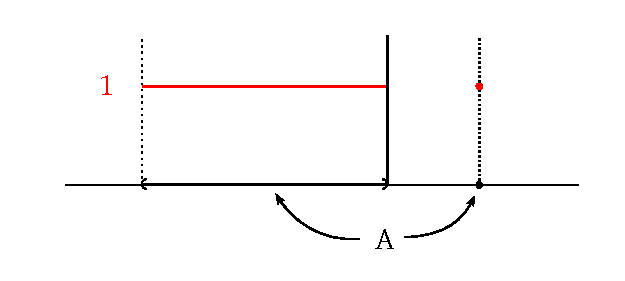
\includegraphics{img/13_characteristic_function.pdf}
    \caption{A characteristic function takes value $1$ inside a set $A$ which can be an interval (left) or a single point (right)}
    \label{img:charf}
  \end{center}
\end{figure}

\begin{remark}
  Let $A = (a', b')$ with $a \leq a' < b' \leq b$.
  Then $\chi_{(a',b')} \in \tau[a,b]$. Also for $x \in [a,b]$, it holds that $\chi_{\set{x}} = \tau[a,b]$.
  Therefore
  \begin{itemize}
    \item every linear combination of characteristic functions of open subintervals ($a',b'$) of $[a,b]$ or
    \item characteristic functions of one-point sets $\chi_{\set{x}}, x \in [a,b]$
  \end{itemize}
  are step functions on $[a,b]$. Compare with Figure~\ref{img:linchar}.

  \begin{figure}[t]
    \begin{center}
      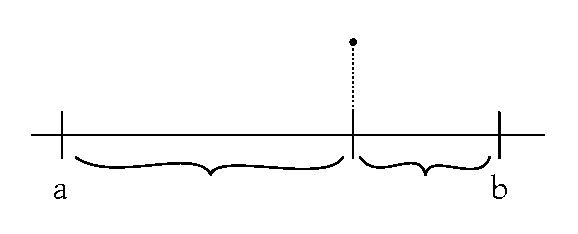
\includegraphics{img/13b_char_function_as_step_function.pdf}
      \caption{Linear combinations of characteristic functions are step functions}
      \label{img:linchar}
    \end{center}
  \end{figure}

  \[ \sum_{j=1}^n \alpha_j \chi_{(a_j,b_j)} + \sum_{k=1}^m \beta_k \chi_{\set{x_k}} \in \tau[a,b] \]
  On the opposite, $f \in \tau[a,b]$, hence
  \[ f|_{(x_{j-1},x_j)} \underbrace{=}_{j=1,\dots,n} c_j \text{ and } f(x_j) \underbrace{=}_{j=0,\dots,n} d_j \]
  \[ f = \sum_{j=1}^n c_j \chi_{(x_{j-1},x_j)} + \sum_{j=0}^n d_j \chi_{\set{x_j}} = (*) \]
  for $x \in (x_{j-1}, x_j)$, $\xi_{(x_{j-1},x_j)}(x) = 1$.
  \[ \chi_{(x_{l-1},x_l)}(x) = 0 \text{ for } l \neq j \]
  \[ \chi_{\set{x_l}}(x) = 0 \text{ for } l = 0, \dots, n \]
  i.e. $\sum_{j=1}^n c_l \chi_{(x_{l-1},x_l)}(x) + \sum_{l=0}^n d_j \chi_{\set{x_l}}(x) = c_j \cdot 1 + 0 = c_j$
  hence $(*) = c_j$ on $(x_{j-1}, x_j)$. Therefore $f \in \tau[a,b] \iff f$ is linear combination of characteristic functions
  of open intervals or one-pointed sets.
\end{remark}

\subsection{Limit points}

\index{Limit point}
\begin{definition} % Definition 4
  Let $X$ be a metric space $A \subseteq X$ and $x \in X$ is an accumulating point\footnote{An accumulation point has 3 equivalent definitions (sequence, intersection, infinitely many elements in sphere).} of $A$. % Accumulation point is defined on a set. Accumulation value is defined for a sequence.
  Let $f: A \to \mathbb R$. Let $d$ be the metric of $X$. We say, $f$ has limit $c \in \mathbb R$ in $x$ ($\lim_{\xi\to x} f(\xi) = c$) if
  \[ \forall \varepsilon > 0 \exists \delta > 0 \forall \xi \in A \forall \xi \neq x: d(\xi, x) < \delta \implies \card{f(\xi) - c} < \varepsilon \]
\end{definition}

\begin{remark}
  Recognize that $\xi \neq x$ relaxes the precondition.
  The preconditions look similar to continuity, but fewer $\xi$ need to satisfy a certain criterion.
\end{remark}

\begin{remark}
  $x \in A$ and $c = f(x) \implies f$ is continuous in $x$.

  We usually consider $A = [a,b] \subseteq \mathbb R$, $x \in [a,b]$.

  It is possible, that $f$ in $x$ has a limit, $x \in A$ and $c = \lim_{\xi\to x} f(\xi) \neq f(x)$.
  Compare with Figure~\ref{img:limfuncvalue}.
\end{remark}

\begin{figure}[t]
  \begin{center}
    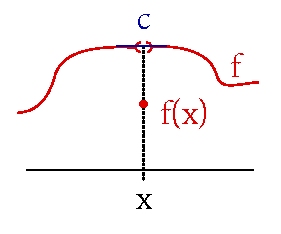
\includegraphics{img/14_special_case_limit_value_not_function_value.pdf}
    \caption{The limit value must not be necessarily the function value}
    \label{img:limfuncvalue}
  \end{center}
\end{figure}

\begin{definition} % Definition 5
  Now let $A \subseteq \mathbb R$ and $x$ is a accumulation point of $A$.
  Let $f: A \to \mathbb R$ be given. We say $f$ has a right-sided limit $c$ in $x$
  with $c = \lim_{\xi \to x^+} f(\xi) = c$ if
  \[ \forall \varepsilon > 0 \exists \delta > 0: \forall \xi \in A, \xi > x: \card{\xi - x} = \xi - x < \delta \implies \card{f(\xi) - c} < \varepsilon \]

  Compare with Figure~\ref{img:def5}.
  The left-sided limit follows analogously (with $\xi < x$).
  \[ c = \lim_{\xi \to x^+} f(\xi) \qquad d = \lim_{\xi \to x^-} f(\xi) \]

  \begin{figure}[t]
    \begin{center}
      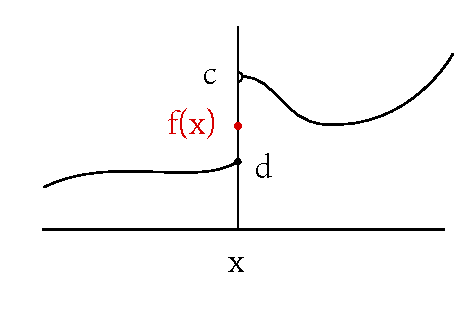
\includegraphics{img/14b_def5.pdf}
      \caption{Left-sided and right-sided limit}
      \label{img:def5}
    \end{center}
  \end{figure}
\end{definition}

\begin{lemma}[Sequence criterion for limits of functions] % Lemma 5
  \label{lemma5}
  Let $f: A \subseteq X \to \mathbb R$ be given. $x$ is an accumulation point of $A$.
  Then
  \begin{align*}
    \lim_{\xi \to x} f(\xi) = c \iff &\forall (\xi_n)_{n\in\mathbb N}: \xi_n \in A, \xi_n \neq x \text{ and } \\
                                     &\lim_{n\to\infty} \xi_n = x \text{ it holds that } \lim_{n\to\infty} f(\xi_n) = c
  \end{align*}
  For one-sided limits $A \subseteq \mathbb R$,
  \begin{align*}
    c = \lim_{\xi\to x^{+}} f(\xi) \iff &\forall (\xi_n)_{n\in\mathbb N}: \xi \in A: \xi_n > x \text{ with } \\
                                        &\lim_{n\to\infty} \xi_n = x \text{ it holds that } \lim_{n\to\infty} f(\xi_n) = c
  \end{align*}
\end{lemma}

\begin{proof}
  See Analysis 1 lecture notes.
\end{proof}

\begin{remark}
  Due to condition $\xi_n \neq x$, the function value must not necessarily match the limit point.
\end{remark}

\begin{remark}
  Attention! We, therefore, use two different definitions of limits.
\end{remark}

\begin{lemma}[Cauchy criterion of limits of functions] % Lemma 6
  \label{cauchy-crit}
  Let $f: A \subseteq X \to \mathbb R$. Let $x$ be an accumulation point of $A$.
  Let $X$ be a metric space.

  \emph{$f$ has a limit in $x$} if and only if $\forall \varepsilon > 0 \exists \delta > 0 \forall \xi, \eta \in A$
  \[
    (\xi \neq x \land \eta \neq x \land d(\xi, x) < \delta \land d(\eta, x) < \delta)
    \implies \card{f(\xi) - f(\eta)} < \varepsilon
  \]
  Analogously for one-sided limits with $A \subseteq \mathbb R$.
  Additionally, we need the constraint that $\xi > x$ and $\eta > x$ for $\lim_{\xi \to x^+} f(\xi)$.
  And accordingly, $\xi < x$ and $\eta < x$ for $\lim_{\xi \to x^-} f(\xi)$.
\end{lemma}

\begin{proof}
  \begin{description}
    \item[$\implies$] 
      Let $c = \lim_{\xi\to x} f(\xi)$ and let $\varepsilon > 0$ be chosen arbitrarily.
      Then there exists $\delta > 0$ such that $d(\xi,x) < \delta$ and $\xi \neq x$
      \[ \implies \card{f(\xi) - c} < \frac\varepsilon2 \]
      For $\xi, \eta$: $d(\xi, x) < \delta$ and $d(\eta, x) < \delta$ with $\xi, \eta \neq x$
      is therefore
      \[ \card{f(\xi) - f(\eta)} = \card{f(\xi) - c + c - f(\eta)} \leq \card{f(\xi) - c} + \card{f(\eta) - c} < \frac\varepsilon2 + \frac\varepsilon2 = \varepsilon \]
    \item[$\impliedby$]
      Assume the Cauchy criterion holds. We show that
      \begin{enumerate}
        \item for every sequence $(\xi_n)_{n\in\mathbb N}$, $\xi_n \in A \setminus \set{x}$ with $\lim_{n\to\infty} \xi_n = x$ it holds that
        $(f(\xi_n))_{n\in\mathbb N}$ is a Cauchy sequence in $\mathbb R$ and therefore convergent in $\mathbb R$.
        \item all Cauchy sequences have the \emph{same} limit $c$.
      \end{enumerate}
      We prove (1.)

      Let $(\xi_n)_{n\in\mathbb N}$ be as above. Let $\varepsilon > 0$ be arbitrary.
      and $N_{\varepsilon}$ large enough such that $\forall n \in N_{\varepsilon}: d(\xi_n, x) < \delta$
      ($\delta$ chosen appropriately to $\varepsilon$ according to the Cauchy criterion).

      By the Cauchy criterion, $\card{f(\xi_n) - f(\xi_m)} < \varepsilon$ for all $m,n \geq N_{\varepsilon}$.
      Therefore $(f(\xi_n))_{n\in\mathbb N}$ is a Cauchy sequence in $\mathbb R$.
      If $\mathbb R$ is complete, then there exists $c = \lim_{n\to\infty} f(\xi_n)$. QED.

      We prove (2.)

      Let $\xi_n \to x$ as above and $\xi_n' \to x$ as above and $c = \lim_{n\to\infty} f(\xi_n)$ as well as $c' = \lim_{n\to\infty} f(\xi_n')$. Let $\varepsilon > 0$ be arbitrary, $N_{\varepsilon}$ such that $n \geq N_{\varepsilon} \implies \card{f(\xi_n) - c} < \frac{\varepsilon}{3}$ and $N_{\varepsilon}' \in \mathbb N$ such that $n \geq N_{\varepsilon}' \implies \card{f(\xi_n') - c'} < \frac\varepsilon3$.

      Furthermore choose $\delta > 0$ such that
      \[ d(\xi, x) < \delta \land d(\eta, x) < \delta \implies \card{f(\xi) - f(\eta)} < \frac{\varepsilon}{3} \]
      (because of the Cauchy criterion).
      $M_{\varepsilon}$ such that 
      \[ n \geq M_{\varepsilon} \implies d(\xi_n, x) < \delta \land M_{\varepsilon}': n \geq M_{\varepsilon}' \implies d(\xi_n', x) < \delta \]
      Let $n \geq \max\set{N_{\varepsilon}, N_{\varepsilon}', M_{\varepsilon}, M'_{\varepsilon}}$.

      \dateref{2018/04/10}

      Then
      \[ \card{c - c'} \leq \underbrace{\card{c - f(\xi_n)}}_{< \frac\varepsilon3} + \underbrace{\card{f(\xi_n) - f(\xi'_n)}}_{< \frac\varepsilon3} + \underbrace{\card{f(\xi'_n) - c'}}_{< \frac\varepsilon3} \qquad \forall \varepsilon > 0 \]
      Hence, $c = c'$.
      We have shown that $\exists c \in \mathbb R: \forall (\xi_n)_{n \in \mathbb N}$ with $\lim_{n\to\infty} \xi_n = x$ it holds that
      $\lim_{n\to\infty} f(\xi_n) = c$. So $\lim_{\xi\to\infty} f(\xi) = c$ because of Lemma~\ref{lemma5}. QED.
  \end{description}
\end{proof}

\subsection{Regulated functions}

\index{Regulated function}
\begin{definition}[Regulated function] % Definition 6
  Let $a < b$, $f: [a,b] \to \mathbb R$. We call $f$ a \emph{regulated function on $[a,b]$} if
  \begin{enumerate}
    \item $\forall x \in (a,b)$, $f$ in $x$ has a right-sided and a left-sided limit.
    \item in $x = a$, $f$ has a right-sided limit.
    \item in $x = b$, $f$ has a left-sided limit.
  \end{enumerate}

  \[ \mathcal R[a,b] = \setdef{f: [a,b] \to \mathbb R}{f \text{ is a regulated function}} \]
\end{definition}

\begin{definition}[Equivalent definition]
  \begin{enumerate}
    \item $\forall x \in [a,b)$, $f$ has a right-sided limit in $x$
    \item $\forall x \in (a,b]$, $f$ has a left-sided limit in $x$
  \end{enumerate}
\end{definition}

\begin{example}
  Let $f$ be continuous in $[a,b]$.
  Let $\varphi \in \tau[a,b]$ be a regulated function. Then $\varphi \in \mathcal R[a,b]$.

  Rationale:

  Let $x_0 = a < x_1 < \dots < x_n = b$ and $\varphi|_{(x_{j-1}, x_j)} = c_j$.

  Let $x \in [a,b]$ be chosen arbitrarily.

  \begin{description}
    \item[Case 1]
      Let $x \in (x_{j-1}, x_j)$ for some $j \in \set{1, \dots, n}$
      \[ \implies \lim_{\xi\to x} \varphi(\xi) = c_j \]
      Choose $\delta$ small enough such that $(x - \delta, x + \delta) \subseteq (x_{j-1}, x_j)$.
      $\forall \xi$ with $\xi \in (x - \delta, x + \delta)$ it holds that
      \[ \card{\varphi(\xi) - c_j} = 0 \]
    \item[Case 2]
      Let $x = x_j$ for $j = 1, \dots, n-1$.
      \[ \implies \lim_{\xi \to x_j^+} \varphi(\xi) = c_{j+1} \]
      \[ \lim_{\xi \to x_j^-} \varphi(\xi) = c_j \]
      Compare with Figure~\ref{img:regf}.
      \begin{figure}
        \begin{center}
          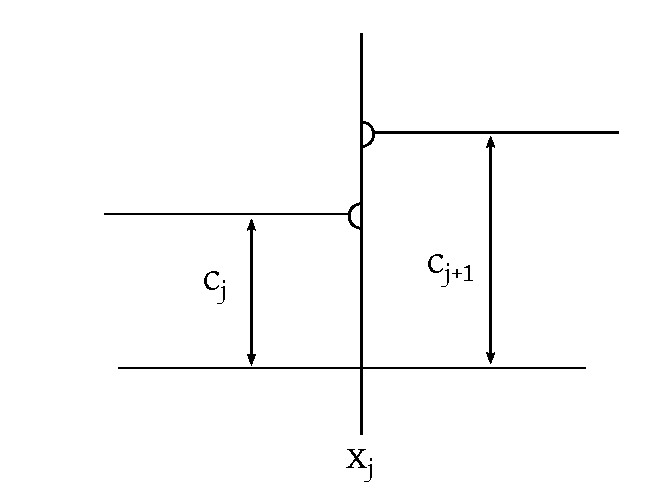
\includegraphics{img/15_regulated_function.pdf}
          \caption{Regulated function}
          \label{img:regf}
        \end{center}
      \end{figure}
    \item[Case 3]
      Let $x = x_0 = a \implies \lim_{\xi \to a^+} \varphi(\xi) = c_1$.
      \[ x = x_n = b \implies \lim_{\xi \to b^-} \varphi(\xi) = c_n \]
  \end{description}

  Let $f: [a,b] \to \mathbb R$ be monotonically increasing oder monotonically decreasing.
  Then $f \in \mathcal R[a,b]$. The proof will be done in the practicals.
\end{example}

\subsection{Bounded functions on bounded sets}

\begin{definition}[Boundedness] % Definition 7
  Let $X \neq \emptyset$ be a set.
  $f: X \to \mathbb K$ with $\mathbb K = \mathbb R$ or $\mathbb K = \mathbb C$.
  We say: $f$ is bounded on $X$, if $f(X) \subseteq \mathbb K$ is a bounded set in $\mathbb K$.
  Hence, $\exists m \geq 0: \card{f(x)} \leq m \forall x \in X$.
  We let,
  \[ \mathcal B(X) = \setdef{f: X \to \mathbb K}{f \text{ is bounded}} \]
  $\mathcal B(X)$ has vector space structure.
  $f, g \in \mathcal B(X), \lambda \in \mathbb K$.
  \[ (f + g)(x) = f(x) + g(x) \]
  \[ (\lambda \cdot f)(x) = \lambda \cdot f(x) \]
  $f + g \in \mathcal B(X)$ and $\lambda f \in \mathcal B(X)$.
  Let $\card{f(x)} \leq m \forall x \in X$ and $\card{g(x)} \leq m' \forall x \in X$.
  Then
  \[ \card{(f + g)(x)} = \card{f(x) + g(x)} \leq \card{f(x)} + \card{g(x)} \leq m + m' \]
\end{definition}

\begin{remark}
  It is very interesting, that $X$ does not require any kind of algebraic structure.
\end{remark}

We let
\[
  \norm{f}_{\infty}
  = \sup\underbrace{\setdef{\card{f(x)}}{x \in X}}_{\text{bounded in } \mathbb R}
  = \min\setdef{m \geq 0}{\card{f(x)} \leq m \forall x \in X}
\]
Some work is required to show that $\norm{\cdot}_{\infty}$ is a norm on $\mathcal B(X)$.

Hence, $(\mathcal B(X), \norm{\cdot}_{\infty})$ is a normed vector space.
Convergence in $\mathcal B(X)$: It holds that $f_n \to f$ in $(\mathcal B(X), \norm{\cdot}_{\infty})$
if and only if $\forall \varepsilon > 0 \exists N \in \mathbb N: n \geq N \implies \norm{f_n - f}_{\infty} < \varepsilon$.

\[ \norm{f_n - f}_{\infty} < \varepsilon \iff \sup\set{\card{f_n(x) - f(x)}: x \in X} \]
\[ \iff \card{f_n(x) - f(x)} \leq \varepsilon \forall x \in X \]
Hence, $f_n \to f$ in $(\mathcal B(X), \norm{\cdot}_{\infty}) \iff \forall \varepsilon > 0 \exists N \in \mathbb N: n \geq N \implies \card{f_n(x) - f(x)} \leq \varepsilon \forall x \in X$.
We say \enquote{$f_n$ converges \emph{uniformly} to $f$ on $X$}.

\begin{theorem}[Approximation theorem for regulated function] % Satz 1
  \label{approxthmreg}
  Let $f: [a, b] \to \mathbb R$. Then $f \in \mathcal R[a,b] \iff \forall \varepsilon > 0$ there exists some step function $\varphi \in \tau[a,b]$ such that $\card{\varphi(x) - f(x)} < \varepsilon \forall x \in [a,b]$ ($\norm{\varphi - f}_{\infty} < \varepsilon$).

  Especially $\varepsilon_n = \frac1n$ and $\varphi_n$ as above.
  Then $\norm{\varphi_n - f}_{\infty} < \frac1n$, hence $f = \lim_{n\to\infty} \varphi_n$ uniformly on $[a,b]$.
\end{theorem}

\begin{proof}\hfill{}
  \begin{description}
    \item[Direction $\implies$.] 
      Let $f \in \mathcal R[a,b]$.

      Proof by contradiction. We negate our hypothesis:
      \begin{align}
        \exists \varepsilon > 0: \forall \varphi \in \tau[a,b] \exists x \in [a,b]: \card{\varphi(x) - f(x)} \geq \varepsilon
        \label{neghypo}
      \end{align}
      Assume \eqref{neghypo} holds for $f \in [a,b]$.
      We construct nested intervals $[a_n, b_n]$ with $[a_{n+1}, b_{n+1}] \subseteq [a_n, b_n]$
      and $b_{n+1} - a_{n+1} = \frac12 (b_n - a_n)$ and \eqref{neghypo} holds on $[a_n, b_n] \forall n \in \mathbb N$.
      Hence $\forall \varphi \in \tau[a_n, b_n] \exists x \in [a_n, b_n]$ such that $\card{\varphi(x) - f(x)} \geq \varepsilon$.
      This is what we want to show.

      Let $a_0 = a$ and $b_0 = b$. Then \eqref{neghypo} holds on $[a_0, b_0]$ by assumption.
      $n \to n+1$: Construction of $[a_{n+1}, b_{n+1}]$. Let $m_n = \frac12(a_n + b_n)$.

      \begin{claim}
        \eqref{neghypo} holds either on $[a_n, m_n]$ or on $[m_n, b_n]$.
      \end{claim}

      \begin{proof}
        Because if the opposite of \eqref{neghypo} holds on $[a_n, m_n]$ as well as $[m_n, b_n]$,
        then there exists $\varphi_n^1 \in \tau[a_n, m_n]$ with $\card{\varphi_n^1(x) - f(x)} < \varepsilon \forall x \in [a_n, m_n]$
        and if the opposite of \eqref{neghypo} holds on $[m_n, b_n]$:
        \[ \exists \varphi_n^2 \in \tau[m_n, b_n]: \card{\varphi_n^2(x) - f(x)} < \varepsilon \forall x \in [m_n, b_n] \]
        \[
          \varphi^n(x) \coloneqq \begin{cases}
            \varphi_n^1(x) & \text{ if } x \in [a_n, m_n] \\
            \varphi_n^2(x) & \text{ if } x \in (m_n, b_n]
          \end{cases}
        \]
        Then $\varphi^n$ is piecewise constant, hence $\varphi^n \in \tau[a_n, b_n]$ and
        \[
          \card{\varphi^n(x) - f(x)} = \begin{cases}
            \underbrace{\card{\varphi_1^n(x) - f(x)}}_{< \varepsilon}  & \text{ for } x \in [a_n, m_n] \\
            \underbrace{\card{\varphi_2^n(x) - f(x)}}_{< \varepsilon}  & \text{ for } x \in [m_n, b_n]
          \end{cases}
        \]
        Therefore, $\card{\varphi^n(x) - f(x)} < \varepsilon$, which contradicts with \eqref{neghypo} on $[a_n, b_n]$.
        We conclude: \eqref{neghypo} holds on $[a_n, m_n]$ or on $[m_n, b_n]$.
      \end{proof}

      Now, choose $[a_{n+1}, b_{n+1}]$ as one of the subintervals in which \eqref{neghypo} holds.
      Let $X \in \bigcap_{n \in \mathbb N} [a_n, b_n]$ (by completeness of $\mathbb R$).

      \begin{description}
        \item[Case $\mathbf{x \in (a,b)}$] 
          Let $x \in (a, b)$. Let $\varepsilon$ as above such that \eqref{neghypo} holds on every interval $[a_n, b_n]$.
          Let $c_+ = \lim_{\xi \to x^+} f(\xi)$ and $c_- = \lim_{\xi \to x^-} f(\xi)$ (feasible, because $f \in \mathcal R[a,b]$).

          By the limit property, $\exists \delta > 0: \card{\xi - x} < \delta$ and $\xi < x$, then $\card{f(\xi) - c_-} < \varepsilon$
          and $\card{\xi - x} < \delta$ and $x < \delta$ then $\card{f(\xi) - c_+} < \varepsilon$.

          Additionally, choose $\delta$ sufficiently small enough such that $(x - \delta, x + \delta) \subseteq [a, b]$.
          \[
            \hat\varphi(\xi) \coloneqq \begin{cases}
              0 & \text{ for } \xi \in [a,b] \setminus (x - \delta, x + \delta) \\
              c_- & \text{ for } \xi \in (x - \delta, x) \\
              c_+ & \text{ for } \xi \in (x, x + \delta) \\
              f(x) & \text{ for } \xi = x
            \end{cases}
          \]

          \begin{figure}[t]
            \begin{center}
              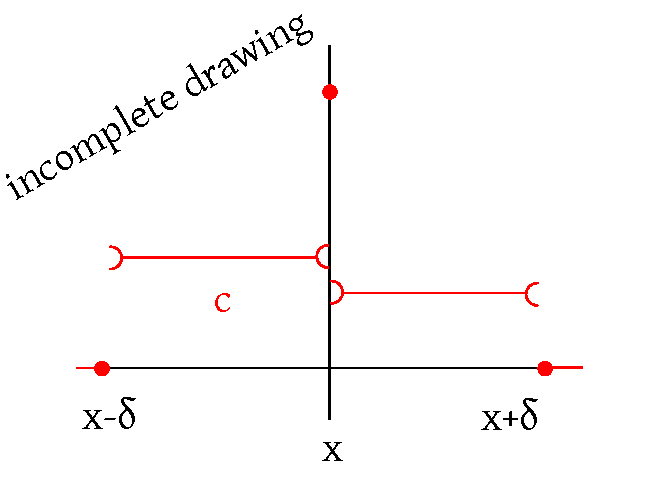
\includegraphics{img/16_construction.pdf}
              \caption{Construction of $\hat\varphi(\xi)$}
              \label{img:hatvarphi}
            \end{center}
          \end{figure}

          Compare with Figure~\ref{img:hatvarphi}.
          $\hat{\varphi} \in \tau[a,b]$ and
          \[
            \forall \xi \in (x - \delta, x + \delta):
            \card{\hat\varphi(\xi) - f(\xi)} = \begin{cases}
              \underbrace{\card{c_- - f(\xi)}}_{< \varepsilon} & \text{ for } \delta \in (x - \delta, x) \\
              \underbrace{\card{f(x) - f(x)}}_{= 0} & \text{ for } \xi = x \\
              \underbrace{\card{c_+ - f(\xi)}}_{< \varepsilon} & \text{ for } \xi \in (x, x + \delta)
            \end{cases}
          \]
          Hence, $\card{\hat\varphi(\xi) - f(\xi)} < \varepsilon$.
          Now let $N$ be sufficiently large enough such that $[a_N, b_N] \subseteq (x - \delta, x + \delta)$
          (possible because $([a_n, b_n])_{n \in \mathbb N}$ gives nested intervals tightening on $x$).
          Then for $[a_N, b_N]$:
          \[ \hat\varphi|_{[a_N, b_N]} \in \tau[a_N, b_N] \]
          and $\forall \xi \in [a_N, b_N] \subseteq (x - \delta, x + \delta): \card{\hat{\varphi}(\xi) - f(\xi)} < \varepsilon$.
          This contradicts with \eqref{neghypo} on $[a_N, b_N]$.
        \item[Case $\mathbf{x = a}$ and $\mathbf{x = b}$]
          Is analogous to one-sided limits.
      \end{description}
    \item[Direction $\impliedby$.]
      Let $f = \lim_{n\to\infty} \varphi_n$ be uniform on $[a,b]$.

      \begin{claim}
        $\forall x \in [a,b)$ there exists a right-sided limit of $f$ in $x$.
      \end{claim}

      \begin{proof}
        Let $\varepsilon > 0$ be arbitrary. $N \in \mathbb N$ sufficiently large such that
        $\card{f(\xi) - \varphi_N(\xi)} < \frac\varepsilon2 \forall \xi \in [a,b]$.
        $\varphi_N$ is piecewise constant. Choose $\delta > 0$ such that
        $\varphi_N|_{(x, x+\delta)} = c$.
        Now let $\xi, \eta \in (x, x+\delta)$ be chosen arbitrarily.
        Then
        \begin{align*}
          \card{f(\xi) - f(\eta)} &\leq |{f(\xi) - \underbrace{c}_{= \varphi_N(\xi)}}| + |{\underbrace{c}_{= \varphi_N(\eta)} - f(\eta)}| \\
            &= |{\underbrace{f(\xi) - \varphi_N(\xi)}_{< \frac\varepsilon2}}| + |{\underbrace{\varphi_N(\eta) - f(\eta)}_{< \frac\varepsilon2}}|
            < \varepsilon
        \end{align*}
        Therefore $f$ has a right-sided limit in $x$ by the Cauchy criterion.
        $f$ has left-sided limit in every point.
      \end{proof}
      $x \in (a, b]$ follows analogously.
  \end{description}
\end{proof}


\begin{corollary}
  Every regulated function $f \in \mathcal R[a,b]$ is bounded.
\end{corollary}

\begin{proof}[Rationale]
  Let $\varphi \in \tau[a,b]$ with $\norm{f - \varphi}_{\infty} < 1$.
  $\varphi$ is bounded, hence $\exists m \in [0, \infty)$:
  $\card{\varphi(x)} \leq m \forall x \in [a,b]$.
  Then $\card{f(x)} \leq \card{f(x) - \varphi(x)} + \card{\varphi(x)} < 1 + m \forall x \in [a,b]$,
  hence $f \in \mathcal B[a,b]$.
  \[ \mathcal R[a,b] \subseteq \mathcal B[a,b] \]
\end{proof}

\begin{corollary}
  Let $f \in \mathcal R[a,b] \iff f = \sum_{j=0}^\infty \psi_j$ with $\psi_j \in \tau[a,b]$ and the series converges uniformly on $[a,b]$.
\end{corollary}

\begin{proof}\hfill{}
  \begin{description}
    \item[Direction $\impliedby$.]
      Let $f = \sum_{j=0}^\infty \psi_j$ with uniform convergence.
      Let $\varphi_n \coloneqq \sum_{j=0}^n \psi_j \in \tau[a,b]$ and $f = \lim_{n\to\infty} \varphi_n$ uniform on $[a,b] \xRightarrow{Theorem~\ref{approxthmreg}} f \in \mathcal R[a,b]$.
    \item[Direction $\implies$.]
      Let $f \in \mathcal R[a,b]$ and $f = \lim_{n\to\infty} \varphi_n$ with $\varphi_n \in \tau[a,b]$ (by Theorem~\ref{approxthmreg}).
      \begin{align*}
        \psi_0 &= \varphi_0 \\
        \psi_j &= \varphi_j - \varphi_{j-1} \qquad \text{ for } j \geq 1 \\
        \sum_{j=0}^n \psi_j &= \varphi_0 + \sum_{j=1}^n (\varphi_j - \varphi_{j-1}) = \varphi_0 + \sum_{j=1}^n \varphi_j - \sum_{j=0}^{n-1} \varphi_j = \varphi_n
      \end{align*}
      converges uniformly to $f$.
  \end{description}
\end{proof}

\section{Integration of regulated functions}

\begin{definition}[Definition with a theorem] % Definition and Saetzchen 8
  Let $f \in \mathcal R[a,b]$ and $\varphi_n \in \tau[a,b]$ with $f = \lim_{n\to\infty} \varphi_n$ is uniform on $[a,b]$.
  We let
  \[ \int_a^b f(x) \, dx = \lim_{n\to\infty} \int_a^b \varphi_n(x) \, dx \]
  for the integral of $f$ on $[a,b]$.

  Theorem: This limit (on the right-hand side) always exists and is independent of the particular choice of the approximating sequence.
\end{definition}

\begin{proof}
  $\varphi_n$ is chosen as above.
  \[ i_n = \int_a^b \varphi_n \, dx \]
  Show: $i_n$ is Cauchy sequence in $\mathbb R$.

  \dateref{2018/04/12}

  Let $\varepsilon > 0$ be chosen arbitrary. Choose $N \in \mathbb N$ such that
  \[ n \geq N \implies \norm{f - \varphi_n}_{\infty} < \frac{\varepsilon}{2 (b - a)} \]
  For $n,m \geq N$ it holds for $x \in [a,b]$ that
  \[ \card{\varphi_n(x) - \varphi_m(x)} \leq \card{\varphi_n(x) - f(x)} + \card{f(x) - \varphi_m(x)} \]
  \[
    \leq \norm{\varphi_n - f}_\infty + \norm{f - \varphi_m}_{\infty}
    < \frac{\varepsilon}{2 (b - a)} + \frac{\varepsilon}{2 (b - a)} = \frac{\varepsilon}{b - a}
  \]
  $\card{\varphi_n - \varphi_m}$ is a step function.
  \[ \card{\varphi_n - \varphi_m} \leq \frac{\varepsilon}{b - a} \cdot \underbrace{\chi_{[a,b]}}_{\in \tau[a,b]} \]

  Integral for subsequence is monotonous:
  \[
    \card{i_n - i_m} = \card{\int_a^b \varphi_n \, dx - \int_a^b \varphi_m \, dx}
    = \card{\int_a^b (\varphi_n - \varphi_m) \, dx} \underbrace{\leq}_{\text{Lemma~\ref{lem4}}} \int_a^b \card{\varphi_n - \varphi_m} \, dx
  \] \[
    \underbrace{<}_{\text{by monotonicity}}
    \int_a^b \frac{\varepsilon}{b - a} \cdot \chi_{[a,b]} \, dx
    = \frac{\varepsilon}{b - a} \underbrace{\int_a^b \chi_{[a,b]}}_{1 \cdot (b - a)} \, dx
    = \varepsilon
  \]
  So $(i_n)_{n \in \mathbb N}$ is a Cauchy sequence.
  $\mathbb R$ is complete, hence $i = \lim_{n\to\infty} i_n$ exists.

  Uniqueness: (dt. \foreignlanguage{german}{mithilfe des Reissverschlussprinzips})

  Let $(\varphi_n)_{n \in \mathbb N}$, $(\Phi_n)_{n \in \mathbb N}$ be two sequences of step functions,
  converging uniformly towards $f$.
  \[
    i_n = \int_a^b \varphi_n \, dx \quad \text{ and } \quad j_n = \int_a^b \Phi_n \, dx
  \] \[
    i = \lim_{n\to\infty} i_n \qquad j = \lim_{n\to\infty} j_n
  \]
  Show that $i = j$.

  Now we construct a sequence $(\mu_n)_{n \in \mathbb N}$ of step functions.
  \[ \underbrace{(\varphi_1, \Phi_1, \varphi_2, \Phi_2, \dots)}_{(\mu_n)_{n \in \mathbb N}} \]
  $\mu_n$ is a sequence of step functions converging uniformly towards $f$ (the proof is left as an exercise to the reader).

  Because of part~1 of the proof:
  \[ m_n = \int_a^b \mu_n \, dx \text{ converges with limit } m \]
  $(i_n)_{n\in\mathbb N}$ as well as $(j_n)_{n \in \mathbb N}$ are subsequences of $(m_n)_{n \in \mathbb N}$.
  Hence $i = \lim_{n\to\infty} i_n = m = \lim_{n\to\infty} j_n = j$.
\end{proof}

\begin{theorem}[Elementary properties of an integral]
  Let $f, g \in \mathcal R[a,b]$, $\lambda, \mu \in \mathbb R$.
  Then
  \begin{description}
    \item[Linearity]
      \[ \lambda f + \mu g \in \mathcal R[a,b] \text{ and } \int_a^b (\lambda f + \mu g) \, dx = \lambda \int_a^b f \, dx + \mu \int_a^b g \, dx \]
    \item[Monotonicity]
      If $f(x) \leq g(x) \forall x \in [a,b]$ ($f \leq g$) it holds that
      \[ \int_a^b f \, dx \leq \int_a^b g \, dx \]
    \item[Boundedness]
      $\card{f} \in \mathcal R[a,b]$  and
      \[ \card{\int_a^b f \, dx} \leq \int_a^b \card{f} \, dx \]
  \end{description}
\end{theorem}
\begin{proof}\hfill{}
  \begin{description}
    \item[Linearity.] 
      Let $x \in [a,b)$ and $c_+ = \lim_{\xi \to x_+} f(\xi)$ as well as $d_+ = \lim_{\xi \to x_+} g(\xi)$
      ($f,g \in \mathcal R[a,b]$). Then
      \[
        \lim_{\xi \to x^+} (\lambda f(\xi) + \mu g(\xi))
          = \lambda \lim_{\xi \to x^+} f(\xi) + \mu \lim_{\xi \to x^+} g(\xi)
          = \lambda c_+ + \mu d_+
      \]
      exists. Analogously for the left side, hence $\lambda f + \mu g \in \mathcal R[a,b]$.

      \begin{claim}
        Let $\varphi_n, \Phi_n \in \tau[a,b]$ with $\varphi_n \to f$ and $\Phi_n \to g$ is uniform on $[a,b]$.
        Hence $\lambda \varphi_n + \mu \Phi_n \to \lambda f + \mu g$ is continuous on $[a,b]$.
      \end{claim}

      \begin{proof}
        Let $\varepsilon > 0$ be arbitrary,
        $N$ such that $n \geq N \implies \norm{\varphi_n - f}_{\infty} < \frac{\varepsilon}{2(\card{\lambda} + 1)}$
        and $M$ such that $n \geq M \implies \norm{\Phi_n - g}_{\infty} < \frac{\varepsilon}{2(\card{\mu} + 1)}$.

        Then
        \[
          \norm{\lambda \varphi_n + \mu \Phi_n - \lambda f - \mu g}_{\infty}
            \leq \card{\lambda} \norm{\varphi_n - f}_{\infty}
            + \card{\mu} \norm{\Phi_n - g}_{\infty}
        \] \[
            < \frac{\card{\lambda}}{2(\card{\lambda} + 1)} \cdot \varepsilon + \frac{\card{\mu}}{2(\card{\mu} + 1)} \cdot \varepsilon
            < \frac\varepsilon2 + \frac\varepsilon2 = \varepsilon
        \]
      \end{proof}

      We continue:
      \[
        \int_a^b (\lambda f + \mu g) \, dx = \lim_{n\to\infty} \int_a^b \left(\lambda \varphi_n + \mu \Phi_n\right) \, dx
          = \lim_{n\to\infty} \left(\lambda \int_a^b \varphi_n \, dx + \mu \int_a^b \Phi_n \, dx\right)
      \] \[
        = \lambda \underbrace{\lim_{n\to\infty} \int_a^b \varphi_n \, dx}_{\text{exists}}
        + \mu \underbrace{\lim_{n\to\infty} \int_a^b \Phi_n \, dx}_{\text{exists}}
        = \lambda \int_a^b f \, dx + \mu \int_a^b g \, dx
      \]
    \item[Monotonicity.]
      Show: Let $h \in \mathcal R[a,b]$ with $h \geq 0$ in $[a,b]$.
      Then $\int_a^b h \, dx \geq 0$.

      \begin{claim}
        There exists $(\tilde \varphi_n)_{n\in\mathbb N}$ with $\tilde \varphi_n \to h$ uniform on $[a,b]$
        and $\tilde \varphi_n \geq 0$.
      \end{claim}

      \begin{proof}
        Let $(\varphi_n)_{n\in\mathbb N}$, $\varphi_n \in \tau[a,b]$ with $\varphi_n \to h$ uniform on $[a,b]$.
        We define $\tilde\varphi_n$ such that
        \[ \varphi_n = \sum_{j=1}^{m_n} c_j \chi_{(x_{j-1}, x_j)} + \sum_{j=0}^{m_n} d_j \chi_{\set{x_j}} \]
        \[ \tilde\varphi_n \coloneqq \sum_{j=1}^{m_n} \underbrace{\tilde c_{j}}_{\geq 0} \chi_{(x_{j-1}, x_j)} + \sum_{j=0}^{m_n} \underbrace{h(x_j)}_{\geq 0} \chi_{\set{x_j}} \]
        and $\tilde c_j \coloneqq \max{c_j, 0} \geq 0$.
        So $\tilde \varphi_n \geq 0$.

        For $x = x_l$ ($l \in \set{0, \dots, m_n}$)
        \[
          \card{\tilde \varphi_n(x_l) - h(x_l)}
            = \card{\sum_{j=1}^{m_n} \tilde c_j \underbrace{\chi_{(x_{j-1}, x_j)}(x_l)}_{=0 \text{ bc. } x_l \not\in (x_{j-1}, x_j)} + \sum_{j=0}^{m_n} h(x_j) \underbrace{\chi_{\set{x_j}}(x_l)}_{= \delta_{j,l}} - h(x_l)}
        \] \[
          = \card{h(x_l) - h(x_l)} = 0 \leq \card{\varphi_n(x_l) - h(x_l)}
        \]
        For $x \in (x_{j-1}, x_j)$
        \[
          \card{\tilde\varphi_n(x) - h(x)}
            = \card{\sum_{j=1}^{m_n} \tilde c_j \underbrace{\chi_{(x_{j-1}, x_j)}(x)}_{\delta_{l,j}} + \sum_{j=0}^{m_n} h(x) \cdot \underbrace{\chi_{\set{x_j}}(x)}_{=0 \text{ bc. } x \neq x_j} - h(x)}
        \] \[
          = \card{\tilde c_l - h(x)}
          = \begin{cases}
            \card{c_l - h(x)} & \text{ if } c_l \geq 0 \\
            \card{h(x)} = h(x) & \text{ if } c_l < 0
          \end{cases}
        \] \[
          \leq \begin{cases}
            \card{c_l - h(x)} & \text{ if } c_l \geq 0 \\
            h(x) - c_l & \text{ if } c_l < 0
          \end{cases}
        \] \[
          = \begin{cases}
            \card{\varphi_n(x) - h(x)} & \text{ if } c_l = \varphi_n(x) \geq 0 \\
            \card{h(x) - \varphi_n(x)} & \text{ if } c_l = \varphi_n(x) < 0
          \end{cases}
        \] \[
          = \card{\varphi_n(x) - h(x)}
        \]
        hence, $\card{\tilde\varphi_n(x) - h(x)} \leq \card{\varphi_n(x) - h(x)}$
        for $x \in (x_{l-1}, x_l)$ as well as $x = x_i$,
        hence
        \[ \norm{\tilde\varphi_n - h}_{\infty} \leq \underbrace{\norm{\varphi_n - h}_{\infty}}_{\to 0 \text{ for } n \to \infty} \]
        Hence $\norm{\tilde\varphi_n - h}_{\infty} \to 0$ for $n \to \infty$, hence $\tilde\varphi_n$ converges uniformly to $h$.
        There exists
        \[ \int_a^b h \, dx = \lim_{n\to\infty} \underbrace{\int_a^b \underbrace{\tilde\varphi_n}_{\geq 0} \, dx}_{\geq 0} \geq 0 \]
      \end{proof}

      To show monotonicity, we let $f \leq g$ in $[a,b]$, hence $h = g - f \geq 0$ in $[a,b]$
      \[ \implies 0 \leq \int_a^b h \, dx = \int_a^b g \, dx - \int_a^b f \, dx \]
      \[ \implies \int_a^b f \, dx \leq \int_a^b g \, dx \]
    \item[Boundedness.]
      Consider $\card{f}$. Proving $\card{f} \in \mathbb R[a,b]$ is left as an exercise to the reader.
      \[ f \leq \card{f} \text{ on } [a,b] \xRightarrow{\text{monotonicity}} \int_a^b f \, dx \leq \int_a^b \card{f} \, dx \]
      \[ -f \leq \card{f} \text{ on } [a,b] \xRightarrow{\text{monotonicity}} \int_a^b (-f) \, dx = -\int_a^b f \, dx \leq \int_a^b \card{f} \, dx \]
      \[ \implies \card{\int_a^b f \, dx} \leq \int_a^b \card{f} \, dx \]
  \end{description}
\end{proof}

\begin{remark}
  $\mathcal R[a,b]$ is a vector space.

  \begin{enumerate}
    \item $f, g \in \mathbb R[a,b] \implies \lambda f + \mu g \in \mathcal R[a,b]$.
      $\norm{\cdot}_{\infty}$ is a norm on $\mathcal R[a,b]$.
      ($\mathcal R[a,b], \norm{\cdot}_{\infty}$) is a normed vector space.
      Subspace of ($\mathcal B[a,b], \norm{\cdot}_{\infty}$).
      We will show in the practicals that ($\mathcal R[a,b], \norm{\cdot}_{\infty}$) is complete.
  \end{enumerate}
\end{remark}

\begin{theorem}[Mean value theorem of integration calculus]
  \label{mvt} \label{satz3}
  Let $f$ be continuous on $[a,b]$ and $p \in \mathcal R[a,b]$
  and $p \geq 0$ in $[a,b]$.
  Then $f \cdot p \in \mathcal R[a,b]$ and there exists $\xi \in [a,b]$ such that
  \[ \int_a^b f \cdot p \, dx = f(\xi) \cdot \int_a^b p \, dx \]
\end{theorem}
\begin{proof}
  Let $m = \min\set{f(z): z \in [a,b]}$ (exists because $f$ is continuous and $[a,b]$ is compact).
  \[ M = \max\set{f(z): z \in [a,b]} \]
  \[ f([a,b]) = [m, M] \text{ (by the mean value theorem)} \]
  \[ m \cdot \underbrace{p(x)}_{\geq 0} \leq f(x) \cdot p(x) \leq M \cdot p(x) \]
  By monotonicity,
  \[ m \int_a^b p(x) \, dx \leq \int_a^b fp \, dx \leq M \int_a^b p \, dx \]
  Therefore, there exists $\eta \in [m, M]$.
  \[ \eta \cdot \int_a^b p(x) \, dx = \int_a^b fp \, dx \]
  Mean value theorem: For $\eta \in [m,M]$ there exists $\xi \in [a,b]$ such that
  \[ \eta = f(\xi) \text{ (f is continuous!)} \]
  Hence,
  \[ f(\xi) \int_a^b p \, dx = \int_a^b f \cdot p \, dx \]
  $f \cdot p$ is regulated function (over one-sided limits).
\end{proof}

\begin{lemma} % Lemma 7
  Let $f \in \mathcal R[a,b]$ and $a \leq \alpha < \beta < \gamma \leq b$.
  Then
  \[ f|_{[\alpha,\beta]} \in \mathcal R[\alpha,\beta], f|_{\beta,\gamma} \in \mathcal R[\beta,\gamma] \]
  \[ f|_{[\alpha,\gamma]} \in \mathcal R[\alpha,\gamma] \text{ (immediate over onesided limit)} \]
  \[ \text{and } \int_{\alpha}^\gamma f\, dx = \int_{\alpha}^\beta f \, dx + \int_\beta^\gamma f \, dx \]
  Compare with Figure~\ref{img:posneg}.
\end{lemma}

\begin{figure}
  \begin{center}
    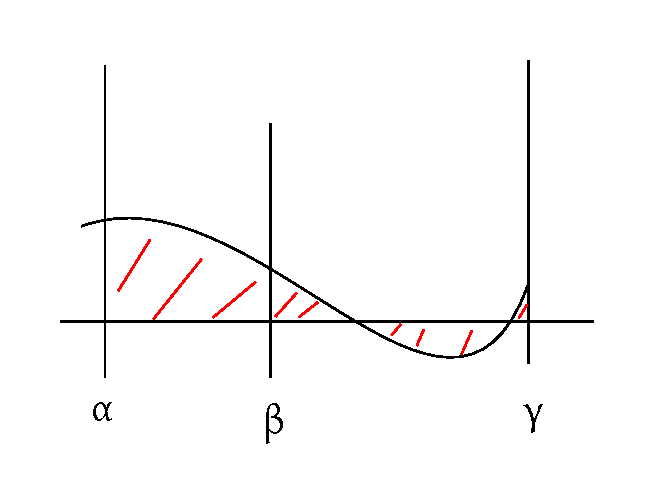
\includegraphics{img/17_posneg_area.pdf}
    \caption{Positive and negative area covered by the integral}
    \label{img:posneg}
  \end{center}
\end{figure}

\begin{proof}
  Show that this statement holds for $\varphi \in \tau[a,b]$.
  Without loss of generality, $\alpha = a, \gamma = b$.
  \[ \gamma = \sum_{j=1}^m c_j \chi_{(x_{j-1}, x_j)} + \sum_{j=0}^m 0 \cdot \chi_{x_j} \]
  The zero represents that this term is not relevant for the integral in any way.
  \begin{description}
    \item[Case 1] 
      $\beta = x_l$ for some $l \in \set{1, \dots, m-1}$
      \[ \int_{\alpha}^\gamma \varphi \, dx = \sum_{j=1}^m c_j (x_j - x_{j-1}) \]
      \[ \int_{\alpha}^\beta \varphi \, dx = \int_{\alpha}^{x_l} \varphi \, dx = \sum_{j=1}^l c_j (x_j - x_{j-1}) \]
      \[ \int_{\beta}^\gamma \varphi \, dx = \int_{x_l}^{\gamma} \varphi \, dx = \sum_{j=l+1}^m c_j (x_j - x_{j-1}) \]
      And now,
      \[ \sum_{j=1}^l c_j (x_j - x_{j-1}) + \sum_{j=l+1}^m c_j (x_j - x_{j-1}) = \sum_{j=1}^m c_j (x_j - x_{j-1}) \]
    \item[Case 2]
      $\beta \in (x_{l-1}, x_l)$ for some $l \in \set{1, \ldots, m}$. Compare with Figure~\ref{img:step18}.
      \begin{figure}[t]
        \begin{center}
          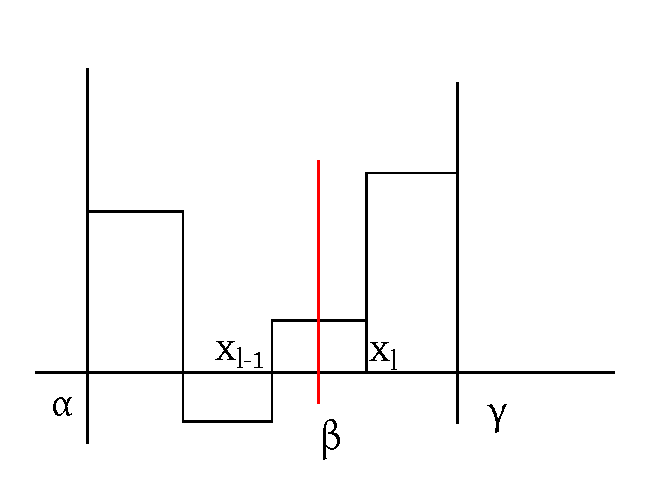
\includegraphics{img/18_step.pdf}
          \caption{Setting for $\beta \in (x_{l-1}, x_l)$}
          \label{img:step18}
        \end{center}
      \end{figure}
      \[ \int_\alpha^\beta \varphi \, dx = \sum_{j=1}^{l-1} c_j (x_j - x_{j-1}) + c_l \cdot (\beta - x_{l-1}) \]
      \[ \int_\beta^\gamma \varphi \, dx = c_l(x_l - \beta)+ \sum_{j=l+1}^m c_j (x_j - x_{j-1}) \]
      Now we consider the addition of these two expressions:
      \[
        \int_{\alpha}^\beta \varphi \,dx + \int_\beta^\gamma \varphi \,dx
      \] \[
        = \sum_{j=1}^{l-1} c_j (x_j - x_{j-1}) + \underbrace{c_l(\beta - x_{l-1}) + c_l (x_l - \beta)}_{= c_l (x_l - x_{l-1})} + \sum_{j=l+1}^m c_j(x_j - x_{j-1})
      \]
      \[ = \sum_{j=1}^m c_j(x_j - x_{j-1}) = \int_{\alpha}^\gamma \varphi \, dx \]
      Let $\varphi_n \in \tau[\alpha,\beta]$ with $\varphi_n \to f$ uniform on $[\alpha, \beta] \implies \varphi_n|_{[\alpha,\beta]} \to f|_{[\alpha,\beta]}$ uniform on $[\alpha,\beta]$ and also $\varphi_n|_{[\beta,\gamma]} \to f|_{[\beta,\gamma]}$ uniform on $[\beta,\gamma]$.
      \[ \int_{\alpha}^\gamma f \, dx = \lim_{n\to\infty} \int_{\alpha}^\gamma \varphi_n \, dx = \lim_{n\to\infty} \left(\int_{\alpha}^\beta \varphi_n \, dx + \int_{\beta}^\gamma \varphi_n \, dx\right) \]
      \[
        = \underbrace{\lim_{n\to\infty} \int_{\alpha}^\beta \varphi_n \, dx}_{\substack{\text{exists because } \\ \varphi_n|_{[\alpha,\beta]} \to f|_{[\alpha,\beta]} \text{uniform}}} + \lim_{n\to\infty} \int_{\beta}^\gamma \varphi_n \, dx
        = \int_{\alpha}^\beta f \, dx + \int_{\beta}^\gamma f \, dx
      \]
  \end{description}
\end{proof}

\begin{remark}[Notation]
  Let $\alpha < \beta$, $\alpha, \beta \in [a,b]$ and $f \in \mathcal R[a,b]$. We let
  \[ \int_{\beta}^\alpha f \, dx \coloneqq -\int_{\alpha}^\beta f \, dx \]
  By this convention,
  \[ \int_{\alpha}^\alpha f \, dx = -\int_{\alpha}^\alpha f \, dx \implies \int_{\alpha}^\alpha f \, dx = 0 \]
\end{remark}

\begin{lemma} % Lemma 8
  \label{lemma8}
  Let $f \in \mathcal R[a,b]$ and $\alpha,\beta,\gamma \in [a,b]$ (without particular order).
  Then
  \[ \int_{\alpha}^\gamma f \, dx = \int_{\alpha}^\beta f \, dx + \int_{\beta}^\gamma f \, dx \]
\end{lemma}

\begin{proof}
  Special case: 2 points are equal
  \[ \alpha = \gamma \implies \int_a^\alpha f \, dx = 0 \]
  \[ \int_\alpha^\beta f \, dx + \int_\beta^\alpha f \, dx = \int_{\alpha}^\beta f \, dx - \int_\alpha^\beta f \, dx = 0 \]
  \[ \beta = \gamma \qquad \beta = \alpha \]

  Case: $\alpha < \beta < \gamma$ follows immediately

  And just as a representative other case: $\alpha < \gamma < \beta$
  \[ \int_{\alpha}^\beta f \, dx \underbrace{=}_{\text{by Lemma~\ref{lemma7}}} \int_{\alpha}^\gamma f \, dx + \underbrace{\int_{\gamma}^\beta f \, dx}_{- \int_{\beta}^\gamma f \, dx} \]
  \[ \int_\alpha^\beta f \, dx + \int_\beta^\gamma f \, dx = \int_\alpha^\gamma f \, dx \]
\end{proof}

\dateref{2018/04/17}

\begin{lemma} % Lemma 9
  \label{lemma9}
  Let $f \in \mathcal R[a,b]$. Then there exists an at most countable set $A \subseteq [a,b]$ such that $f$ is continuous in every point $x \in [a,b] \setminus A$.
\end{lemma}
\begin{proof}
  Let $f \in \mathcal R[a,b]$ and $(\varphi_n)_{n \in \mathbb N}$ with $\varphi_n \in \tau[a,b]$ and $\varphi \to f$ converging uniformly on $[a,b]$.
  \[ \varphi_n = \sum_{j=1}^{m_n} c_j^n \chi_{(X_{j-1}^n, X_j^n)} + \sum_{j=0}^{m_n} d_j^n \chi_{\set{x_j^n}} \]
  \[ x_0^n = a < x_1^n < \ldots < x_{m_n}^n = b \]
  are separating points for $\varphi_n$
  \[ A = \set{X_j^n: n \in \mathbb N, j \in \set{0, \ldots, m_n}} \]
  $A$ is a countable union of finite sets $A_n = \set{x_0^n, x_{m_n}^n}$. A is countable (as unions of finite sets are).

  Now we show: $f$ is continuous in every point $x \in [a,b]: x \not\in A$.
  Let $\varepsilon > 0$ be arbitrary. Choose $N \in \mathbb N$ sufficiently large such that $\norm{\varphi_N - f}_{\infty} < \frac\varepsilon2$. Because $x \in A$, there exists $j \in \set{1, \ldots, m_N}$ such that $x \in (x_{j-1}^N, X_j^N)$ is open.
  Choose $\delta > 0$ such that $(x - \delta, x + \delta) \subset (x_{j-1}^N, x_j^n)$, hence $\forall \xi \in (x - \delta, x + \delta)$ it holds that $\varphi_N(\xi) = c_j^N$. \\
  Now consider $\xi \in (x - \delta, x + \delta)$, hence $\card{\xi - x} < \delta$. Then
  \[ \card{f(\xi) - f(x)} = \card{f(\xi) - \underbrace{\varphi_N(x)}_{c_j^N = \varphi_N(\xi)} + \varphi_N(x) - f(x)} \]
  \[ \leq \underbrace{\card{f(\xi) - \varphi_N(\xi)}}_{\leq \norm{f - \varphi_N}_{\infty}} + \underbrace{\card{\varphi_N(x) - f(x)}}_{\leq \norm{\varphi_N - f}_{\infty}} < \frac\varepsilon2 + \frac\varepsilon2 = \varepsilon \]
  Hence $f$ is continuous in $x$.
\end{proof}

\begin{remark}[Notation]
  Let $f \in \mathcal R[a,b]$. For $x \in [a,b)$, there exists $f_+(x) \coloneqq \lim_{\xi \to x_+} f(\xi)$.
  For $x \in (a,b]$, there exists $f_-(x) \coloneqq \lim_{\xi \to x_-} f(\xi)$.
  Because of Lemma~\ref{lemma9}, it holds that $f_+(x) = f_-(x) = f(x)$ for all $x \in [a,b] \setminus A$ and $A$ is at most countable.
\end{remark}

\index{Right-sided derivative}
\index{Left-sided derivative}
\index{Half-sided derivative}
\begin{definition}[One-sided derivatives] % Definition 9
  Let $g: [a,b] \to \mathbb R$ and $x \in [a,b)$.
  We say $g$ has the \emph{right-sided derivative} $g'_+(x)$ if
  \[ \lim_{\xi \to x_+} \frac{g(\xi) - g(x)}{\xi - x} \eqqcolon g'_+(x) \]
  exists. Analogously we define the left-sided derivative
  \[ g'_-(x) = \lim_{\xi \to x_-} \frac{g(\xi) - g(x)}{\xi - x} \]
  for $x \in (a,b]$. Compare with Figure~\ref{img:lrderiv}.

  \begin{figure}[!h]
    \begin{center}
      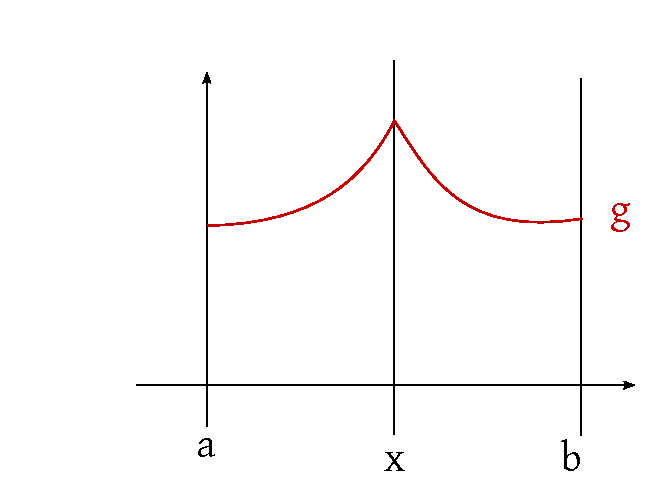
\includegraphics{img/19_left_right_sided_derivative.pdf}
      \caption{In this example, the left- and right-sided derivatives are not equal. $f'_+(x) \neq f'_-(x)$}
      \label{img:lrderiv}
    \end{center}
  \end{figure}
\end{definition}

\begin{remark}
  If $g$ in $x$ has a one-sided derivative, then
  \[ \lim_{\xi \to x_\pm} (g(\xi) - g(x)) = 0 \]
  Hence $g$ is continuous in $x$.
\end{remark}

\begin{remark}
  $g: [a,b] \to \mathbb R$ is differentiable in point $x \in (a,b)$ with derivative $g'(x)$
  $\iff g$ has a left- and right-sided derivative in $x$ and $g'_-(x) = g'_+(x)$ ($= g'(x)$).
\end{remark}

\begin{theorem}[Fundamental theorem of differential/integration calculus, variation 1] % Satz 4
  \label{ftofic}
  Isaac Barrow (1630--1677), Isaac Newton (1642--1726), Gottfried Wilhelm von Leibniz (1646--1716).

  Let $f \in \mathcal R[a,b]$, $\alpha \in [a,b]$ and we define
  \[ F(x) \coloneqq \int_{\alpha}^x f(\xi) \, d\xi \]
  Then $F$ is right-sided differentiable in every point $x \in [a,b)$ and left-sided differentiable in every $x \in (a,b]$.
  Furthermore
  \begin{align}
    \label{ftdi}
    F'_+(x) &= f_+(x) \forall x \in [a,b) \\
    F'_-(x) &= f_-(x) \forall x \in (a,b]
  \end{align}
\end{theorem}

\begin{remark}
  \[ \frac{d}{dx} \left(\int_\alpha^x f \, d\xi\right) = f(x) \]
  for all $x$ such that $f$ is continuous in $x$.
  For those $x$, $F'(x)$ is differentiable in $x$ with $F'(x) = f(x)$.
\end{remark}

\index{Antiderivative}
\begin{definition} % Definition 10
  \label{def10}
  Let $f \in \mathcal R[a,b]$ and $\varphi: [a,b] \to \mathbb R$ such that $\varphi$ is one-sided differentiable on $[a,b]$.
  If $\Phi'_+(x) = f_+(x) \forall x \in [a,b)$ and $\Phi'_-(x) = f_-(x) \forall x \in (a,b]$
  then we call $\Phi$ an antiderivative of regulated function $f$.
\end{definition}

\begin{proof}[Proof of the Theorem~\ref{ftofic}]
  Let $x_1, x_2 \in [a,b]$ be arbitrary. Let $F$ be defined as above. Then
  \[ \card{F(x_2) - F(x_1)} = \card{\int_\alpha^{x_2} f \, d\xi - \int_\alpha^{x_1} f \, d\xi} \]
  \[ = \card{\int_\alpha^{x_2} f \, d\xi + \int_{x_1}^\alpha f \, d\xi} = \card{\int_{x_1}^{x_2} f \, d\xi} \]
  \[ \leq \int_{x_1}^{x_2} \card{f} \, d\xi \leq \int_{x_1}^{x_2} \underbrace{\norm{f}_{\infty}}_{\text{const independent of } \xi} \, d\xi  = \norm{f}_{\infty} \cdot \card{x_2 - x_1} \]
  Hence $F$ is Lipschitz continuous with Lipschitz constant $\norm{f}_{\infty}$. So $F$ is continuous in $[a,b]$.

  One-sided derivatives: Let $x \in [a,b)$ and $\varepsilon > 0$ be arbitrary.
  Choose $\delta > 0$ such that $\forall \xi \in [x, x+\delta)$ it holds that $\card{f(\xi) - f_+(x)} < \varepsilon$.
  For $\xi \in (x, x+\delta)$,
  \[ \card{\frac{F(\xi) - F(x)}{\xi - x} - f_+(x)} = \frac1{\card{\xi - x}} \card{\underbrace{\int_x^\xi f \, dy}_{F(\xi) - F(x)} - \underbrace{f_+(x)(\xi - x)}_{\int_x^\xi \underbrace{f_+(x)}_{\text{const.}} \, dy}} \]
  \[ = \frac{1}{\card{\xi - x}} \card{\int_x^\xi (f - f_+(x)) \, dy} \leq \frac{1}{\card{\xi - x}} \int_x^\xi \underbrace{\card{f(y) - f_+(x)}}_{< \varepsilon} \, dy \]
  \[ y \in (x, \xi) \subseteq (x, x+\delta) \]
  \[ < \frac{1}{\xi - x} \varepsilon \cdot \underbrace{\int_x^\xi 1 \, dy}_{\card{\xi - x}} = \varepsilon \]
  Hence, $F'_+(x) = f_+(x)$.
  Analogously, $F'_-(x) = f_-(x)$ for $x \in (a,b]$.
\end{proof}

\begin{theorem}[Fundamental theorem of differential/integration calculus, variation 2] % Satz 5
  \label{satz5}
  Let $f \in \mathcal R[a,b]$ and $\phi$ is an arbitrary antiderviative of $f$ according to Definition~\ref{def10}.
  For $\alpha, \beta \in [a,b]$ arbitrary,
  \[ \int_\alpha^\beta f \, dx = \phi(\beta) - \phi(\alpha) \]
\end{theorem}

\begin{remark} % TODO in this section, I am mixing \Phi and \phi to denote an antiderivative
  Let $f$ be continuous and $\phi$ be an antiderivative of $f$.
  Hence, $\Phi'(x) = f(x) \forall x \in [a,b]$.
  Then
  \[ \int_{\alpha}^{\beta} \Phi' \, dx = \Phi(\beta) - \Phi(\alpha) \]
  \enquote{Integral of a derivative of $\Phi$ gives $\Phi(\beta) - \Phi(\alpha)$}.
\end{remark}

\begin{lemma} % Lemma 10
  \label{lemma10}
  Let $A \subseteq [a,b]$ countable.
  $f: [a,b] \to \mathbb R$ is continuous and $f$ is differentiable in every point $x \in [a,b] \setminus A$.
  Furthermore let $\card{f'(x)} \leq L$ ($L \geq 0$) for all $x \in [a,b] \setminus A$.
  Then $f$ is Lipschitz continuous on $[a,b]$ with constant $L$, hence
  \[ \card{f(x_2) - f(x_1)} \leq L \card{x_2 - x_1} \forall x_1, x_2 \in [a,b] \]
\end{lemma}
\begin{remark}
  Some people call it \emph{differentiable almost everywhere},
  but this expression collides with a different definition
  pronounced the same way from measure theory.
\end{remark}
\begin{proof}
  Let $x_1, x_2 \in [a,b]$, without loss of generality: $x_1 < x_2$.
  Let $\varepsilon > 0$ be arbitrary. We define
  \[ F_{\varepsilon}(x) = \card{f(x) - f(x_1)} - (L + \varepsilon)(x - x_1) \]
  for $x \in [x_1, b]$.

  Let $\varepsilon > 0$ be arbitrary.
  We prove: $F_{\varepsilon}(x) \leq 0 \forall x \in [x_1, b]$.
  In particular: $F_{\varepsilon}(x_2) \leq 0$. Hence,
  \[ \card{f(x_2) - f(x_1)} \leq (L + \varepsilon)\underbrace{(x_2 - x_1)}_{\card{x_2 - x_1}} \]

  We prove by contradiction:
  Assume there exists $\varepsilon > 0$ and $x_{\varepsilon} > x_1$
  such that
  \begin{align}
    F_{\varepsilon}(x_{\varepsilon}) = \eta > 0
    \label{hash}
  \end{align}

  We recognize:
  Let $A' = [x_1, b] \cap A$ be countable.
  \begin{enumerate}
    \item hence $F_{\varepsilon}(A') \subseteq \mathbb R$ is countable
    \item $F_{\varepsilon}(x_1) = 0$, $F_{\varepsilon}(x_{\varepsilon}) > 0 \implies x_{\varepsilon} > x_1$
    \item $F_{\varepsilon}$ is continuous on $[x_1, b]$.
      It holds that $0 \in F_{\varepsilon}([x_1, x_{\varepsilon}])$ because $0 = F_{\varepsilon}(x_1)$
      and $\eta \in F_{\varepsilon}([x_1, x_{\varepsilon}])$ because $\eta = F_{\varepsilon}(x_{\varepsilon})$.

      By the Intermediate Value Theorem, it follows that $[0, \eta] \subseteq F_{\varepsilon}([x_1, x_{\varepsilon}])$ where $[0, \eta]$ is uncountable.
      $F_{\varepsilon}(A')$ is countable, hence there exists $\gamma \in (0, \eta]$ such that $\gamma = F_{\varepsilon}(y)$ and $\gamma \not\in A'$ ($\gamma > 0$); compare with inequality~\eqref{hash}.
      Hence, $y \not\in A'$. So $f$ in $y$ is differentiable.
      Let $B \coloneqq F_{\varepsilon}^{-1}(\set{\gamma}) \cap \left([x_1, x_{\varepsilon}] \setminus A'\right)$, where we can skip $A'$.
      Then $B \neq \emptyset$.

      $B \subseteq [x_1, x_{\varepsilon}]$ is therefore bounded, $B \neq 0$.
      Hence, $B$ has a supremum. Let $x = \sup{B}$.
      Choose $(y_n)_{n \in \mathbb N}$ with $y_n \in B$ and $y_n \to x$ for $n \to \infty$.
      Because $F_{\varepsilon}$ is continuous,
      \[ \lim_{n\to\infty} \underbrace{F_{\varepsilon}(y_n)}_{\gamma} = F_{\varepsilon}(x) \]
      hence $F_{\varepsilon}(x) = \gamma$. This implies $x \not\in A$.

      Furthermore it holds for $w \in (x, x_\varepsilon]$ that $F_{\varepsilon}(w) > \gamma$.
      Because assume the opposite ($F_{\varepsilon}(w) \leq \gamma$ for $w > x$).
      Furthermore, $F_{\varepsilon}(x_{\varepsilon}) = \eta \geq \gamma$.
      Because of the Intermediate Value Theorem, $\exists y \geq w$ with $F_{\varepsilon}(y) = \gamma$.
      This contradicts with the supremum property of $x$.

      Now let $y \in (x, x_{\varepsilon}]$.
      \begin{align*}
        \varphi(y) &= \frac{F_{\varepsilon}(y) - F_{\varepsilon}(x)}{y - x} \\
          &\underbrace{=}_{\substack{\text{definition of} \\ F_{\varepsilon}}}
          \frac{\card{f(y) - f(x_1)} - \card{f(x) - f(x_1)}}{y - x} - \frac{(L + \varepsilon)(y - x_1 - x + x_1)}{y - x} \\
          &\underbrace{\leq}_{\text{reversed triangle ineq.}} \frac{f(y) - f(x)}{y - x} - (L + \varepsilon)
      \end{align*}
      Because $F_{\varepsilon}(y) > \gamma = F_{\varepsilon}(x)$, $\varphi(y) > 0$ for $y > x$.
      So,
      \[ \frac{\card{f(y) - f(x)}}{y - x} \geq L + \varepsilon \]
      \[ \card{f'(x)} = \lim_{y \to x_+} \card{\frac{f(y) - f(x)}{y - x}} \geq L + \varepsilon \]
      This contradicts with the boundedness of the derivative by $L$ and $f$ is in $x \not\in A$ differentiable.

      So, inequality~\eqref{hash} does not hold. Therefore $\forall x_1, x_2$ with $x_1 < x_2$ in $[a,b]$ and $\forall \varepsilon > 0$,
      \[ \card{f(x_2) - f(x_1)} \leq (L + \varepsilon)\card{x_2 - x_1} \]
      \[ \implies \card{f(x_2) - f(x_1)} \leq L \card{x_2 - x_1} \]
  \end{enumerate}
\end{proof}

\begin{corollary}[Corollary to Lemma~\ref{lemma10}]
  Let $f, g: [a,b] \to \mathbb R$ differentiable for all points $x \in [a,b] \setminus A$
  and $A$ is countable. Furthermore let $f'(x) = g'(x) \forall x \not\in A$.
  Then there exists $K \in \mathbb R$ such that $f(x) = g(x) + K \forall x \in [a,b]$.
\end{corollary}

\begin{proof}
  Let $h = f - g$. Then
  \[ h'(x) = f'(x) - g'(x) = 0 \forall x \in [a,b] \setminus A \]
  By Lemma~\ref{lemma10} with $L = 0$, it follows that
  \[ \card{h(x_1) - f(x_2)} \leq 0 \cdot \card{x_1 - x_2} = 0 \]
  \[ \implies h(x_1) = h(x_2) \forall x_1, x_2 \in [a,b] \]
  Hence, $h(x) = K \in \mathbb R$.
  \[ \implies f(x) = g(x) + h(x) = g(x) + K \]
\end{proof}

\dateref{2018/04/19}

By reference~(*), $\gamma \in [0, \eta)$ (uncountable) and $\gamma \not\in f(A)$ (countable).
\[ \implies \forall u \in [x_1, b) \text{ with } F_{\varepsilon}(u) = \gamma \]
it holds that $u \not\in A$, hence $f$ is differentiable in $u$.

\begin{proof}[Proof of Theorem~\ref{satz5}]
  Let $f \in \mathcal R[a,b]$ and let $\phi$ be an antiderivative of $f$,
  hence $\phi_+' = f_+$, $\phi_-' = f_-$. Let $\alpha \in [a,b]$ be arbitrary.
  By the Theorem variant 1, $F(x) = \int_{\alpha}^x f \, d\xi$ is also an antiderivative of $f$.
  By Lemma~\ref{lemma10}, $\exists K \in \mathbb R: F(x) = \int_{\alpha}^x f \, d\xi = \phi(x) + K$.
  Determine $K$: Let $x = \alpha \implies F(\alpha) = \int_\alpha^\alpha f \, dx = 0 = \phi(\alpha) - K$
  hence $K = \phi(\alpha)$. Hence,
  \[ \int_\alpha^x f \, d\xi = \phi(x) - \phi(\alpha) \]
  Let $x = \beta$.
\end{proof}

\begin{remark}[Remark for the previous corollary]
  $F$, $\phi$ are differentiable on all points $x$ for which $f$ is continuous
  (all of them except for countable many).
  For those $x$, $F'(x) = \varphi'(x) = f(x)$.
\end{remark}

\index{Indefinite integral}
\begin{remark}[Notation]
  Let $f \in \mathcal R[a,b]$. Then
  \[ \int f \, dx \]
  \begin{itemize}
    \item is some particular antiderivative of $f$ (usually some arbitrary chosen)
    \item the set of \emph{all} antiderivatives of $f$
      \[ \int f \, dx = \set{F: F \text{ is antiderivative of f}} \]
      If $F_0$ is some fixed antiderivative, then
      \[ \int f \, dx = \set{F_0 + K: K \in \mathbb R} \]
      Then $\int f \, dx$ is the so-called \emph{indefinite integral of $f$}.
      Notation:
      \[ \int x^k \, dx = \frac{x^{k+1}}{k+1} + c \qquad (k \neq -1) \]
  \end{itemize}
\end{remark}

\begin{table}[!h]
  \begin{center}
    \begin{tabular}{c|c|c}
      $f$ & $F$ & remark \\
    \hline
      $x^\alpha$ & $\frac{x^{\alpha+1}}{\alpha + 1} + c$ & $\alpha \in \mathbb R \setminus \set{-1}$; restrict $x$ \\
        & & such that $x^\alpha$ and $x^{\alpha+1}$ are defined \\
      $x^{-1}$ & $\ln{x} + c$ ($x > 0$) & \\
      $\left(\frac1{-x}\right) \cdot (-1) = x^{-1}$ & $\ln{-x} + c$ ($x < 0$) & \\
      $e^x$ & $e^x$ & \\
      $\sin{x}$ & $-\cos{x}$ & \\
      $\cos{x}$ & $\sin{x}$ & \\
      $\sinh{x}$ & $\cosh{x}$ & \\
      $\cosh{x}$ & $\sinh{x}$ & \\
      $\frac{1}{1 + x^2}$ & $\arctan x$ \\
      $\frac{1}{\sqrt{1 - x^2}}$ & $\arcsin{x}$ & $\card{x} < 1$ \\
      $-\frac{1}{\sqrt{1 - x^2}}$ & $\arccos{x}$ &
    \end{tabular}
  \end{center}
  \caption{Table of antiderivatives}
  \label{tbl:antideriv}
\end{table}

\subsection{Integration methods}

In this chapter, we discuss how to determine the antiderivative of a function.
Usually they are composites of basic functions. Some of these are given in Table~\ref{tbl:antideriv}.

\begin{remark}
  Let $F, G: [a,b] \to \mathbb R$ in $x \in [a,b)$ right-sided differentiable.
  Then also $F \cdot G$ in $x$ is right-sided differentiable and
  \[ (F \cdot G)'_+(x) = F'_+(x) \cdot G(x) + F(x) \cdot G'_+(x) \]
  hence the product law holds.

  Analogously, the same holds for the left-sided derivative.

  Look up the proof in the course Analysis 1.
\end{remark}

\subsubsection{Partial integration}

\index{Partial integration}
\begin{definition}[Partial integration]
  Let $f, g$ be given. Let $F, G$ be its antiderivatives respectively.
  Then $F \cdot G$ is an antiderivative of $F \cdot g + f \cdot G$.

  This is immediate, because
  \[
    (F \cdot G)'_+ = F'_+ \cdot G + F \cdot G'_+
    = f_+ \cdot G + F \cdot g_+ = f_+ G_+ + F_+ \cdot g_+
  \]
  Hence,
  \[
    \int_a^b (F g + f G) \, dx
    = \underbrace{F(b) \cdot G(b) - F(a) G(a)}_{\eqqcolon \left.F \cdot G\right|_a^b}
  \]
  Usually, this is rewritten as
  \[ \int_a^b F \cdot g \, dx = \left. F \cdot G\right|_a^b - \int_a^b f G \, dx \]
  If $F = u$ is continuously differentiable and $G = v$ as well,
  then $f = u'$ and $g = v'$ and the law has the structure
  \begin{framed}
    \[ \int_a^b uv' \, dx = \left.u\cdot v\right|_a^b - \int_a^b u'v \, dx \]
  \end{framed}
\end{definition}

\begin{example}
  Let $a \neq -1$ and $x > 0$.
  \[
    \int \underbrace{x^a}_{v'} \cdot \underbrace{\ln{x}}_{u} \, dx =
    \underbrace{\begin{vmatrix}
      u = \ln{x} & u' = \frac1x \\
      v' = x^\alpha & v = \frac{x^{\alpha+1}}{\alpha + 1}
    \end{vmatrix}}_{\text{scribble notes}}
    \quad
    \frac{x^{\alpha + 1}}{\alpha + 1} \cdot \ln{x} - \int \frac1{x} \cdot \frac{x^{\alpha+1}}{\alpha + 1} \, dx
  \] \[
    = \frac{x^{\alpha+1}}{\alpha + 1} \cdot \ln{x} - \frac{1}{\alpha + 1} \int x^\alpha \, dx
    = \frac{x^{\alpha+1}}{\alpha + 1} \cdot \ln{x} - \frac{1}{(\alpha + 1)^2} x^{\alpha+1}
  \]
\end{example}

\begin{example}
  Let $k \in \set{2,3,4,\ldots}$.
  \[
    \int \cos^k(x) \, dx =
    \begin{vmatrix}
      u = \cos^{k-1}(x) & u' = (k-1) \cdot \cos^{k-2}(x) \cdot (-\sin{x}) \\
      v' = \cos{x} & v = \sin{x}
    \end{vmatrix}
  \] \[
    \cos^{k-1}(x) \sin{x} + (k - 1) \int \cos^{k-2}(x) \cdot \underbrace{\sin^2(x)}_{(1 - \cos^2{x})} \, dx
  \] \[
    = \cos^{k-1}(x) \cdot \sin(x) + (k-1) \int \cos^{k-2}(x) \, dx - (k-1) \int \cos^k(x) \, dx
  \]
  Then we can use the following identity:
  \[
    k \int \cos^k(x) \, dx = \cos^{k-1}(x) \cdot \sin(x) + (k-1) \int \cos^{k-2}(x) \, dx
  \]
  This gives a recursive formula:
  \[
    \int \cos^k(x) \, dx = \frac1k \cos^{k-1}(x) \cdot \frac{k-1}{k} \sin(x) + (k-1) \int \cos^{k-2}(x) \, dx
  \]
  Analogously,
  \[ \int \sin^k(x) \, dx = -\frac1k \sin^{k-1}(x) \cdot \cos(x) + \frac{k-1}{k} \int \sin^{k-2}(x) \, dx \]
  Let $c_m = \int_0^{\frac\pi2} \cos^m(x) \, dx$. Then the following formula holds:
  \begin{align*}
    c_{2n} &= \frac{2n - 1}{2n} \cdot \frac{2n - 3}{2n - 2} \cdot \frac{2n - 5}{2n - 4} \ldots \frac{1}{2} \cdot \frac{\pi}{2} \\
      &= \prod_{k=1}^n \frac{2k - 1}{2k} \cdot \frac{\pi}{2} \\
    c_{2n+1} &= \prod_{k=1}^n \frac{2k}{2k + 1}
  \end{align*}
  \begin{proof}[Proof by induction]
    Let $n = 1$.
    \begin{align*}
      c_2 &= \int_0^{\frac\pi2} \cos^2{x} \, dx = \left.\frac12 \cos{x} \sin{x} \right|_0^{\frac\pi2} + \frac12 \int_0^{\frac\pi2} 1 \, dx = 0 - 0 + \frac\pi4 \\
          &= \underbrace{\prod_{k=1}^1 \frac{2k - 1}{2k}}_{\frac12} \cdot \frac\pi2 \\
      c_1 &= \int_0^{\frac\pi2} \cos{x} \, dx = \left. \sin{x} \right|_0^{\frac\pi2} = 1 - 0 = 1 \\
      \underbrace{\prod_{k=1}^0 \frac{2k}{2k + 1}}_{\text{empty product}} &= 1 \\
    \end{align*}
    We make the induction step $n \to n+1$:
    \begin{align*}
      c_{2(n+1)} &= \left.\frac{1}{2n+2} \cdot \underbrace{\cos^{2n+1}(x)}_{=0 \text{ for } x = \frac\pi2} \cdot \underbrace{\sin(x)}_{=0 \text{ for } x = 0}\right|_{0}^{\frac\pi2} + \frac{2n + 1}{2n + 2} \int_0^{\frac\pi2} \cos^{2n}(x) \, dx \\
        &= \frac{2n+1}{2n+2} \prod_{k=1}^n \frac{2k - 1}{2k} \cdot \frac\pi2 = \prod_{k=1}^{n+1} \frac{2k-1}{2k} \cdot \frac\pi2 \\
    \end{align*}
    $c_{2(n+1)+1}$ analogously.
  \end{proof}
\end{example}

\begin{theorem}[Wallis product]
  John Wallis (1616--1703), result from 1655

  Let $w_n = \prod_{k=1}^n \frac{(2k)^2}{(2k - 1)(2k + 1)} = \frac{2\cdot 2}{1 \cdot 3} \cdot \frac{4 \cdot 4}{3 \cdot 5} \ldots$.
  Then $\lim_{n\to\infty} w_n = \frac\pi2$.
\end{theorem}
\begin{proof}
  \[
    \frac\pi2 \cdot \frac{c_{2n+1}}{c_{2n}}
    = \frac\pi2 \cdot \prod_{k=1}^n \frac{\frac{2k}{2k+1}}{\prod_{k=1}^n \frac{2k-1}{2k} \cdot \frac\pi2}
    = \prod_{k=1}^n \frac{(2k)^2}{(2k-1)(2k+1)} = w_n
  \]
  It remains to show that $\lim_{n\to\infty} \frac{c_{2n+1}}{c_{2n}} = 1$ in $[0, \frac\pi2]$ it holds that $0 \leq \cos{x} \leq 1$.
  \[ \implies \cos^{2n+2}(x) \leq \cos^{2n+1}(x) \leq \cos^{2n}(x) \]
  So, $c_{2n+2} \leq c_{2n+1} \leq c_{2n}$ for $n \geq 1$.
  \[ 1 \geq \frac{c_{2n+1}}{c_{2n}} \]
  \[ \implies 1 \geq \frac{c_{2n+1}}{c_{2n}} \geq \frac{c_{2n+2}}{c_{2n}} = \frac{\prod_{k=1}^{n+1} \frac{2k-1}{2k} \frac\pi2}{\prod_{k=1}^n \frac{2k-1}{2k} \frac\pi2} \]
  \[ = \frac{2n + 2 - 1}{2n + 2} \to 1  \text{ for } n \to \infty \]
  Because of the sandwich lemma for convergent sequences, the intermediate expression must also converge to $1$, hence
  \[ \lim_{n\to\infty} \frac{c_{2n+1}}{c_{2n}} = 1 \qquad \land \qquad \frac\pi2 \cdot \lim_{n\to\infty} \frac{c_{2n+1}}{c_{2n}} = \underbrace{\lim_{n\to\infty}}_{=1} w_n \]
\end{proof}

\subsubsection{Integration by substitution}
\begin{definition}[Integration by substitution]
  Let $f: [a,b] \to \mathbb R$ be continuous.
  Let $t: [\alpha,\beta] \to [a,b]$ be continuously differentiable.
  Let $F$ be an antiderivative of $f$ ($F$ is therefore continuously differentiable).
  Then $F \circ t: [\alpha, \beta] \to \mathbb R$ is also continuously differentiable and the chain rule holds:
  \[ (F \circ t)' = (F' \circ t) \cdot t' = (f \circ t) \cdot t' \]
  Hence $F \circ t$ is an antiderivative of $(f \circ t) \cdot t'$. We apply it to integration:
  \[
    \int_{\alpha}^\beta (f \circ t)(u) \cdot t'(u) \, du
    = (F \circ t)(\beta) - (F \circ t)(\alpha)
    = F(t(\beta)) - F(t(\alpha)) = \int_{t(\alpha)}^{t(\beta)} f(x) \, dx
  \]
  Then we get the substitution integration method:
  \begin{framed}
  \[
    \int_{t(\alpha)}^{t(\beta)} f(x) \, dx = \int_{\alpha}^\beta f(t(u)) \cdot t'(u) \, du
  \]
  \end{framed}
\end{definition}
\begin{remark}[Mnemonic]
  Consider the left-hand side and right-hand side simultaneously.
  Let $x = t(u)$ (expressions inside parentheses). Then $dx = t'(u) \cdot du$ (expressions on the right).
  Let $u = \alpha \implies x = t(\alpha)$ and $u = \beta \implies x = t(\beta)$ (interval boundaries).
\end{remark}

\begin{example}
  \[ \int_0^1 2x \sqrt{1 - x^2} \, dx \]
  Usually we have some expression, we want to substitute with $u$.
  \[ 1 - x^2 = u \qquad x = \sqrt{1 - u} = t(u) \]
  \[ x = 0 = t(1) \qquad x = 1 = t(0) \]
  \[ dx = \frac12 \cdot \frac{1}{\sqrt{1 - u}} \cdot (-1) \, du \]
  \[ \int_0^1 2x \sqrt{1 - x^2} \, dx = \int_1^0 2 \cdot \sqrt{1 - u} \cdot u \cdot \frac12 (-1) \frac{1}{\sqrt{1 - u}} \, du = \int_0^1 \sqrt{u} \, du = \left. \frac{u^{\frac32}}{\frac32} \right|_0^1 = \frac23 \]

  \[
    \int_0^1 2x \sqrt{\underbrace{1 - x^2}_{u}} \, dx =
    \begin{vmatrix}
      u = 1 - x^2 & \\
      x = 0 & \Leftrightarrow u = 1 \\
      x = 1 & \Leftrightarrow xu = 0 \\
      1 \cdot du &= -2x \, dx
    \end{vmatrix}
    = -\int_1^0 \sqrt{u} \, du = \int_0^1 \sqrt{u} \, du
  \]

  In general: we set $h(u) = g(x)$, then $h'(u) \, du = g'(x) \, dx$.
\end{example}

\begin{theorem} % Satz 7
  \label{satz7countable}
  Let $f, \tilde f \in \mathcal R[a,b]$ and $A \subseteq [a,b]$ countable.
  Furthermore $f(x) = \tilde f(x) \forall x \in [a,b] \setminus A$.
  Then
  \[ \int_a^b \card{f - \tilde f} \, dx = 0 \]
  Then it follows especially that
  \[ \int_a^b f \, dx = \int_a^b \tilde f \, dx \]
\end{theorem}

\dateref{2018/04/24}

\begin{proof}
  Show: $r \in \mathcal R[a,b], r \geq 0$. $\int_a^b r \, dx = 0$
  and $r(x) = 0$ for $x \in [a,b] \setminus A$. Then $\int_a^b r \, dx = 0$.
  Let $r$ be as above. First, we show: $r_+(x) = \lim_{\xi\to x_+} r(\xi) = 0 \forall x \in [a,b)$
  and also $r_-(x) = 0 \forall x \in (a,b]$.

  Proof of that: Let $x \in [a,b)$ and $y = r_+(x)$ (exists because $r \in \mathcal R[a,b]$).
  Choose $\delta_n = \frac1n$. $(x, x + \frac1n) \cap [a,b)$ is an open interval with uncountable many points,
  so there is certainly one point in $A$. So there exists $\xi_n \in ((x, x + \frac1n) \cap [a,b)) \setminus A$
  and $\card{\xi_n - x} < \delta_n = \frac1n$.
  Hence, $\lim_{n\to\infty} \xi_n = x$ and $r(\xi_n) = 0$. Therefore, $\lim_{n\to\infty} r(\xi_n) = 0$ where $r(\xi_n) = y = r_+(x)$.

  Analogously, $r_-(x) = 0$ on $(a,b]$.

  Let $\varepsilon > 0$ be arbitrary. We let $A_{\varepsilon} = \setdef{w \in [a,b]}{r(w) > \varepsilon}$.
  We show: $A_{\varepsilon}$ is finite.

  Assume $A_{\varepsilon}$ would have infinitely many points. Choose a sequence $(w_n)_{n \in \mathbb N}$ with $w_n \in A_{\varepsilon}$ and $w_n \neq w_m$ for $n \neq m$ (works because $A_{\varepsilon}$ is infinite). $(w_n)_{n \in \mathbb N}$ is bounded, hence there exists a convergent subsequence $(w_{n_k})_{k \in \mathbb N}$ with $x = \lim_{k\to\infty} w_{n_k} \in [a,b]$ and $w_{n_k} \in [a,b]$.

  Either $(w_{n_k})$ contains infinitely many sequence element $w_{n_k} < x$ (variant (a)) or infinitely many $w_{n_k} > x$ (variant (b)). Let variant b hold without loss of generality.

  Combine all $w_{n_k} > x$ to one subsequence $(w_{n_{k_l}})_{l \in \mathbb N}$. This gives $\lim_{l\to\infty} w_{n_{k_l}} = x$ and $w_{n_{k_l}} > x$, thus $\lim_{l\to\infty} \underbrace{r(w_{n_{k_l}})}_{\geq \varepsilon \text{ because } w_{n_{k_l}} \in A_{\varepsilon}} = r_+(x) = 0$. This gives a contradiction. $A_{\varepsilon}$ must be finite.

  Consider
  \[ A_{\frac1n} = \set{w_1^n, \dots, w_{m_n}^n} \]
  finite. Let $\varphi_n = \sum_{k=1}^{m_n} r(w_k^n) \cdot \chi_{\set{w_k^n}} \in \tau[a,b]$.

  For $x = w^n_k \in A_{\frac1n}$
  \[ \varphi_n(w_k^n) = \sum_{k=1}^{m_n} r(w_k^n) \cdot \underbrace{\chi_{\set{w_k^n}} (w_j^n)}_{\delta_{jk}} = r(w_j^n) \]
  so $\card{\varphi_n(x) - r(x)} = 0 \forall x \in A_{\frac1n}$.
  Let $x \in [a,b] \setminus A_{\frac1n}$. Then it holds $0 \leq r(x) < \frac1n$ and for $x \not\in A_{\frac1n}$, $\varphi(x) = 0$.
  Therefore,
  \[ \card{r(x) - \varphi(x)} = r(x) < \frac1n \]
  hence $\norm{r - \varphi_n}_{\infty} < \frac1n$. This means that $\varphi_n \to r$ uniformly on $[a,b]$.
  Therefore
  \[ \lim_{n\to\infty} \underbrace{\int_a^b \varphi_n \, dx}_{= 0} = \int_a^b r \, dx = 0 \]

  Now we want to finish the proof of our theorem: Let $r(x) = \card{f(x) - \tilde f(x)} \geq 0$ and $r(x) = 0$ for $x \not\in A$.
  So, $\int_a^b \card{f - \tilde f} \, dx = 0$ (first part proven).
  \[ \card{\int_a^b f \, dx - \int_a^b \tilde f \, dx} = \card{\int_a^b (f - \tilde f) \, dx} \leq \int_a^b \card{f - \tilde f} \, dx = 0 \]
  \[ \implies \int_a^b f\, dx = \int_a^b \tilde f \, dx \]
  Second part proven.
\end{proof}

\begin{lemma} % Lemma 11
  Let $f \in \mathcal R[a,b]$. Then $f_+ \in \mathcal R[a,b]$ and also $f_- \in \mathcal R[a,b]$.
\end{lemma}
\begin{proof}
  Only for $f_+$: First, we show: Let $x \in [a,b)$.
  \[ f_+(x) = \lim_{\xi \to x_+} f(\xi) = \lim_{\xi \to x_+} f_+(x) \]
  (the plus is important on the right-hand side!).

  Proof of this: Let $\varepsilon > 0$ be arbitrary. Then there exists $\delta > 0$ such that
  $\forall \xi \in (x, x + \delta)$: $\card{f(\xi) - f_+(x)} < \frac\varepsilon2$.
  Now let $z \in (x, x + \delta)$ be arbitrary chosen. For $z$ there exists $\xi \in (z, x + \delta)$ because $f_+(z)$ exists.
  Compare with Figure~\ref{img:xz}.

  \begin{figure}[t]
    \begin{center}
      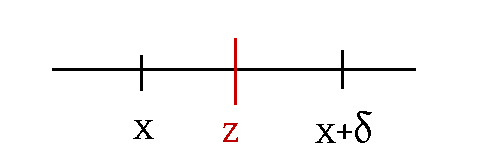
\includegraphics{img/20_x_z.pdf}
      \caption{$\xi$ must be sufficiently close enough to $z$ such that $\card{f(\xi) - f_+(z)} \leq \frac\varepsilon2$.}
      \label{img:xz}
    \end{center}
  \end{figure}

  \[ \card{f_+(z) - f_+(x)} \leq \card{f_+(z) - f(\xi)} + \card{f(\xi) - f_+(x)} < \frac\varepsilon2 + \frac\varepsilon2 \]
  so $f_+(x) = \lim_{z \to x_+} f_+(z)$.

  It remains to show: $f_+$ has left-sided limits.
  Let $x \in (a,b]$ be arbitrary and $f_-(x) = \lim_{\xi \to x_-} f(\xi)$. We show: $f_-(x) = \lim_{\xi \to x_-} f_+(x)$ (again: the plus is important).

  Let $\varepsilon > 0$ be arbitrary. Choose $\delta > 0$ such that $\forall z \in (x - \delta, x)$, $\card{f(z) - f_-(x)} < \frac\varepsilon2$.

  \begin{figure}[t]
    \begin{center}
      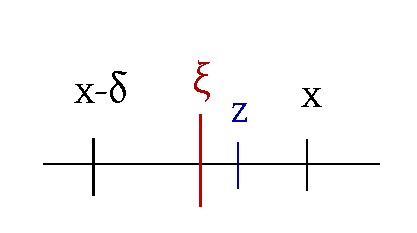
\includegraphics{img/21_xi_z.pdf}
      \caption{$\xi$ and $z$}
      \label{img:xiz}
    \end{center}
  \end{figure}

  Now let $\xi \in (x - \delta, x)$ (compare with Figure~\ref{img:xiz}) and choose $x > z > \xi$ with the property that $\card{f(z) - f_+(\xi)} < \frac\varepsilon2$ (feasible because $f$ in $\xi$ has a right-sided limit):
  \[
    \card{f_+(\xi) - f_-(x)}
    \leq \underbrace{\card{f_+(\xi) - f(z)}}_{< \frac\varepsilon2} + \underbrace{\card{f(z) - f_-(x)}}_{< \frac\varepsilon2}
  \]
  because of the choice of $\delta$ and $z \in (\xi, x) \subseteq (x - \delta, x)$.

  Hence, $\lim_{\xi \to x_-} f_+(\xi) = f_-(x)$. Analogously for $f_-$
\end{proof}

\begin{remark}
  \[ \lim_{\xi \to x_+} f_+(\xi) = f_+(x) \]
  \[ \lim_{\xi \to x_-} f_-(\xi) = f_-(x) \]
  from the proof. So $f_+$ is right-sided continuous and $f_-$ is left-sided continuous.
\end{remark}

\begin{lemma} % Lemma 12
  Let $f \in \mathcal R[a,b]$. Then
  \[ \int_a^b f \, dx = \int_a^b f_+ \, dx = \int_a^b f_- \, dx \]
\end{lemma}

\begin{proof}
  For $f_+$:
  \[ f, f_+ \in \mathcal R[a,b] \]
  $\forall x \in [a,b]$ with $f$ is continuous in $x$,
  \[ f(x) = \lim_{\xi\to x} f(\xi) = \lim_{\xi\to x_+} f(\xi) = f_+(x) \]
  $f$ has at most countable many discontinuity points. By Satz~\ref{satz7countable},
  \[
    \int_a^b \card{f - f_+} \, dx = 0
    \quad \text{ and accordingly } \quad
    \int_a^b f \, dx = \int_a^b f_+ \, dx
  \]
\end{proof}

\subsection{Improper integrals}

Let $I$ be an interval in $\mathbb R$ with marginal points $a$ and $b$ with $-\infty \leq a < b \leq +\infty$.
Let $f$ be a regulated function on $I$.
We define
\begin{enumerate}
  \item If $I = [a,b)$, $\int_a^b f \, dx = \lim_{\beta \to b_-} \int_a^\beta f \, dx$
  \item If $I = (a,b]$, $\int_a^b f \, dx = \lim_{\alpha \to a_+} \int_\alpha^b f \, dx$
  \item If $I = (a,b)$, $\int_a^b f \, dx = \lim_{\alpha \to a_+} \int_\alpha^c f \, dx + \lim_{\beta \to b_-} \int_c^\beta f \, dx$
\end{enumerate}
for an arbitrarily chosen $c \in (a,b)$ under the constraint that the corresponding limits in $\mathbb R$ exist.

Standard examples will follow:
\begin{example}
  Let $s > 1$.
  \[ \int_1^\infty x^{-s} \, dx = \lim_{\beta \to \infty} \int_1^\beta x^{-s} \, dx = \left.\lim_{\beta \to \infty} \left(\frac{1}{-s + 1} x^{-s+1}\right) \right|_1^\beta \]
  \[ = \frac1{1 - s} \cdot \underbrace{\lim_{\beta \to \infty} \frac{1}{\beta^{\underbrace{s-1}_{> 0}}}}_{= 0} - \frac{1}{1 - s} \cdot 1 = \frac{1}{s-1} \]
  Compare with Figure~\ref{img:xs}.
  \begin{figure}[t]
    \begin{center}
      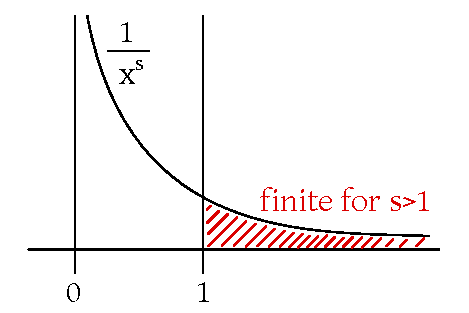
\includegraphics{img/21b_1_by_xs.pdf}
      \caption{The function $\frac{1}{x^s}$ for $s > 1$}
      \label{img:xs}
    \end{center}
  \end{figure}
\end{example}

\begin{example}
  Let $s < 1$.
  \[
    \int_0^1 x^{-s} \, dx = \lim_{\alpha \to 0_+} \int_\alpha^1 x^{-s} \, ds
    = \left. \lim_{\alpha\to 0_+} \frac{1}{-s + 1} x^{-s+1} \right|_\alpha^1
  \] \[
    = \frac1{1 - s} - \frac1{1 - s} \cdot \underbrace{\lim_{\alpha \to 0} \alpha^{\overbrace{1 - s}^{> 0}}}_{= 0} = \frac1{1 - s}
  \]
  Compare with Figure~\ref{img:xs1}.
  \begin{figure}[t]
    \begin{center}
      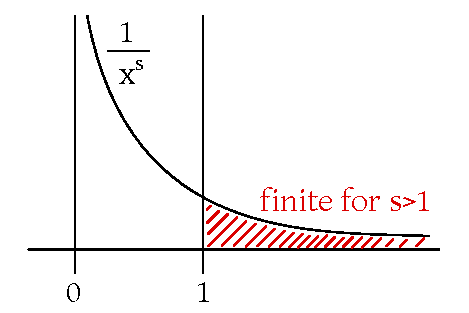
\includegraphics{img/21b_1_by_xs.pdf}
      \caption{The function ${x^s}$ for $s < 1$}
      \label{img:xs1}
    \end{center}
  \end{figure}

  For $s = 1$, neither $\int_0^1 \frac1x \, dx$ nor $\int_1^\infty \frac1x \, dx$ exists.
\end{example}

\begin{example}
  For $c > 0$,
  \[ \int_0^\infty e^{-cx} \, dx = \lim_{\beta \to \infty} \int_0^\beta e^{-cx} \, dx = \left. \lim_{\beta \to \infty} \left(-\frac1c\right) \cdot e^{-cx} \right|_0^\beta - \frac1c \cdot \underbrace{\lim_{\beta \to \infty} e^{-c\beta}}_{= 0} + \frac1c = \frac1c \]
\end{example}

\begin{theorem}[Direct comparison test for improper integrals] % Satz 8
  \label{dctii}
  In German, \enquote{\foreignlanguage{german}{Majorantenkriterium f\"ur uneigentliche Intergale}}.

  Let $f, g$ be regulated functions on $I$ and
  \[ \card{f(x)} \leq g(x) \forall x \in I \]
  Assume $\int_a^b g \, dx$ exists as improper integral. Then also the following improper integrals exist:
  \[ \int_a^b \card{f} \, dx \text{ and } \int_a^b f \, dx \]
  In German, $g$ is called \foreignlanguage{german}{Majorante} of $f$ (there is no equivalent terminology in English).
\end{theorem}

\begin{proof}
  Without loss of generality, let $I = [a,b)$.
  Let $G(\beta) = \int_a^\beta g \, dx$. We know that $\lim_{\beta \to b_-} G(\beta)$ exists.
  By Lemma~\ref{cauchy-crit} (Cauchy criterion for existence of limits):
  Let $\varepsilon > 0$ be arbitrary, then there exists a left-sided neighborhood $U$ of $b$
  ($U = (b - \delta, b)$ if $b < \infty$ and $U = (M, \infty)$ if $b = \infty$)
  with $u,v \in U$, then $\card{G(v) - G(u)} < \varepsilon$.
  \[
    \card{G(v) - G(u)} = \card{\int_a^v g \, dx - \int_a^u g \, dx}
      = \card{\int_u^a g \, dx + \int_a^v g \, dx}
      = \card{\int_u^v g \, dx}
  \]
  Let $F(\beta) = \int_a^\beta \card{f} \, dx$.
  Analogously as for $G$, $F(v) - F(u) = \int_u^v \card{f} \, dx$.
  Let $u,v \in U$. Then
  \[
    \card{F(v) - F(u)} = \card{\int_u^v \card{f} \, dx} \leq \card{\int_u^v g \, dx}
      = \card{G(v) - G(u)} < \varepsilon
  \]
  hence by the Cauchy criterion for $F$:
  $\lim_{\beta\to b_-} F(\beta)$ exists, so there exists $\int_a^b \card{f} \, dx$ as improper integral.
  The same applies for the existence of $\int_a^b f \, dx$.
\end{proof}

\begin{example}
  The cardinal sine function is defined as
  \[ \sinc(x) = \frac{\sin{x}}{x} \]
  \[ \lim_{x\to 0} \frac{\sin{x}}{x} = 1 \qquad \sinc(0) = 1 \]
  So $\sinc(x)$ is continuous on $\mathbb R$.
  \[ \int_0^\infty \frac{\sin{x}}{x} \, dx = \underbrace{\int_0^1 \underbrace{\frac{\sin{x}}{x}}_{\text{continuous}} \, dx}_{\text{exists}} + \int_1^\infty \frac{\sin{x}}{x} \, dx \]
  How about $\int_1^\infty \frac{\sin(x)}{x} \, dx$?
  \[
    \lim_{\beta\to\infty} \int_1^\beta \frac{\sin{x}}{x} \, dx =
      \begin{vmatrix}
        u = \frac1x & u' = -\frac1{x^2} \\
        v' = \sin{x} & v = -\cos{x}
      \end{vmatrix}
      = \lim_{\beta\to\infty} \left[
        -\frac1x \cos{x}
      \right]_1^\beta - \int_1^\beta \frac{\cos{x}}{x^2} \, dx
  \] \[
    = \cos(1) - \lim_{\beta\to\infty} \int_1^\beta \frac{\cos(x)}{x^2} \, dx
  \] \[
    \card{\frac{\cos(x)}{x^2}} \leq \frac1{x^2} \text{ on } [1, \beta]
  \]
  and $\int_1^\infty \frac1{x^2} \, dx$ exists.
  So $g(x) = \frac1{x^2}$ is a majorant of $\frac{\cos(x)}{x^2}$ and by Theorem~\ref{dctii},
  $\lim_{\beta\to\infty} \int_1^\beta \frac{\cos(x)}{x^2} \, dx$ eixsts.

  Attention! $\int_0^\infty \card{\frac{\sin(x)}{x}} \, dx$ does not exist. Is not Lebesgue integrable.
\end{example}

\index{Euler's Gamma function}
\index{Gamma function}
\begin{definition} % Definition 11
  Let $x > 0$.
  We call $\Gamma$ \emph{Euler's Gamma function}.
  \[ \Gamma(x) \coloneqq \int_0^\infty t^{x - 1} e^{-t} \, dt \]
\end{definition}

\begin{remark}
  The improper integral in the definition of the $\Gamma$-function exists for all $x > 0$.
\end{remark}

\dateref{2018/04/26}

Euler's $\Gamma$-function exists for all $x > 0$:
\[ \int_0^1 t^{x-1} e^{-t} \,dt \]
for $0 < x \leq 1$:
\[ t^{x-1} \cdot \underbrace{e^{-t}}_{\leq 1} \leq t^{x-1} \text{ and } \underbrace{\int_0^1 t^{\overbrace{x-1}^{\in (-1,0]}} \, dt}_{\text{exists}} \]
also exists $\int_0^1 t^{x-1} e^{-t} \, dt$ because of the direct comparison criterion.
For $x \geq 1$, $t^{x-1} e^{-t}$ is continuous on $[0,1]$, hence $\int_0^1 t^{x-1} e^{-t} \, dt$ exists.

\begin{claim}
  Let $x > 0$ be fixed. $\exists c > 0$ such that
  \[ t^{x-1} e^{-t} \leq c \cdot e^{-\frac t2} \forall t \in [0,\infty) \]
\end{claim}

\begin{proof}
  \[ \lim_{t\to\infty} \underbrace{t^{x-1}}_{\text{polynomially in } t} \cdot \underbrace{e^{-t}}_{\text{exponentially } \to 0} = 0 \]
  Also there exists $L > 1$, such that $\forall x > L: t^{x-1} e^{-t/2} < 1$ on $[1,L]$ (which is a compact interval) continuous.
  So there exists $M > 0$ such that $t^{x-1} e^{-\frac t2} \leq M \forall t \in [1,L]$.
  Let $c = \max\set{M, 1}$. Therefore it holds on $[1,L]$ and also on $(L,\infty)$.
  \[ t^{x-1} e^{-\frac t2} \leq c \]
  Multiply with $e^{-\frac t2} > 0$, then $t^{x-1} \cdot e^{-t} \leq ce^{-\frac t2} \forall t \in [1,\infty)$.
  \[ c \int_1^\infty e^{-\frac t2} \, dt \]
  exists.
  By the direct comparison test, we get $\int_1^\infty t^{x-1} e^{-t} \, dt$ exists.
\end{proof}

\begin{lemma} % Lemma 13
  \label{lemma13}
  For all $x > 0$,
  \[ \Gamma(x + 1) = x \cdot \Gamma(x) \qquad \text{ (functional equation of the $\Gamma$-function)} \]
  Especially with $\Gamma(1) = 1$ it holds that $\Gamma(n+1) = n!$ for all $n \in \mathbb N_0$.
\end{lemma}

\begin{proof}
  \[ \Gamma(x + 1) = \int_0^\infty t^{x+1-1} e^{-t} \, dt = \int_0^\infty t^{x} e^{-t} \, dt \]
  \begin{align*}
    &= \begin{vmatrix} u = t^x & u' = x \cdot t^{x-1} \\ v' = e^{-t} & v = -e^{-t} \end{vmatrix} \\
    &= \underbrace{\left. -t^x \cdot e^{-t} \right|_0^\infty}_{\substack{= 0 \text{ on the upper bound} \\ = 0 \text{ on the lower bound}}}
    + \int_0^\infty x \cdot t^{x-1} \cdot e^{-t} \, dt = x \int_0^\infty t^{x-1} e^{-t} \, dt = x \Gamma(x)
  \end{align*}
  \[ \Gamma(1) = \int_0^\infty \underbrace{t^{1-1}}_{=1} \cdot e^{-t} \, dt = \left. -e^{-t} \right|_0^\infty = 1 \]
  \[ \Gamma(n+1) = n \cdot \Gamma(n) = n \cdot (n - 1) \Gamma(n-1) = n \cdot (n-1) \cdot \ldots \cdot 1 \cdot \underbrace{\Gamma(1)}_{=1} = n! \]
\end{proof}

\begin{figure}[t]
  \begin{center}
    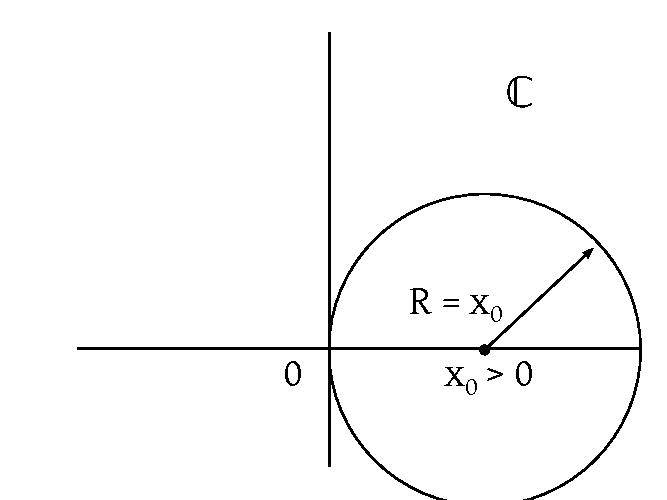
\includegraphics{img/22_gamma_on_C.pdf}
    \caption{$\Gamma$ on $\mathbb C$}
    \label{img:gamma}
  \end{center}
\end{figure}

\begin{remark}
  There exists a power series $\Gamma(x) = \sum_{n=0}^\infty a_n (x - x_0)^n$.
  $\Gamma(z)$ is also defined for $z \in \mathbb C$ with $\Re{z} > 0$.
  Compare with Figure~\ref{img:gamma}.
\end{remark}

\subsection{Young's inequality}

Some important inequalities in integration theory follow.

\index{Young's inequality}
\begin{theorem}[Young's inequality] % Satz 9
  Let $f: [0, \infty) \to [0,\infty)$ be continuous differentiable, strictly monotonically increasing with $f(0) = 0$ and $f$ is unbounded.
  Then $f: [0, \infty) \to [0,\infty)$ bijective and $f^{-1}: [0,\infty) \to [0,\infty)$ is strictly monotonically increasing and continuous.
  Let $a, b \geq 0$ be given. Then
  \[ ab \leq \int_0^a f(x) \, dx + \int_0^b f^{-1}(y) \, dy \]
  Equality is given if and only if, $b = f(a)$ or $a = f^{-1}(b)$.
  Compare with Figure~\ref{img:young}.
\end{theorem}

\begin{figure}[t]
  \begin{center}
    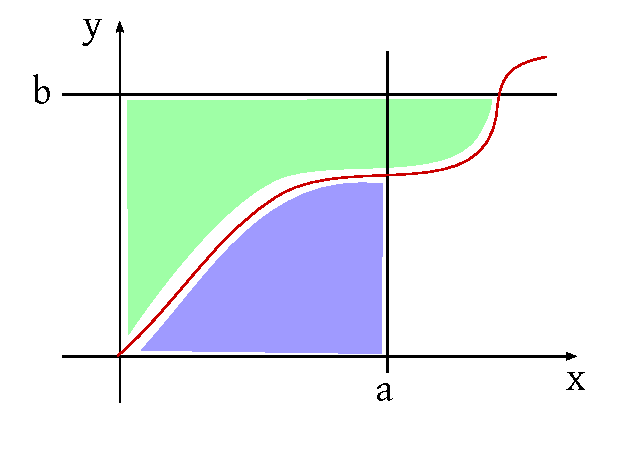
\includegraphics{img/23_young.pdf}
    \caption{Young's inequality visualized. The blue area denotes $\int_0^\alpha f \, dx$ and $\int_0^b f^{-1}(y) \, dy$ is the green area.}
    \label{img:young}
  \end{center}
\end{figure}

\begin{remark}
  The inverse function $f^{-1}$ can be retrieved by considering reflection along $f(x) = x$.
\end{remark}

\begin{proof}
  Let $f:[0,\infty) \to [0,\infty)$ be as above.
  Let $x_1 \neq x_2$. Without loss of generality $x_1 < x_2$.
  Then $f(x_1) < f(x_2) \implies f$ is injective.
  Surjectivity: $f(0) = 0$, hence $0 \in f([0,\infty])$.
  Let $\eta > 0$ be arbitrary. Because $f$ is unbounded, there exists $z \in (0,\infty)$ with $f(z) > \eta$.
  $f(0) = 0 < \eta < f(z)$.

  By the Intermediate Value Theorem ($f$ is continuous), there exists $\xi \in (0,z)$ with $f(\xi) = \eta$.
  So $f$ is surjective.
  \[ f^{-1}: [0,\infty) \to [0,\infty) \]
  \emph{Monotonicity:} Let $y_1 < y_2$. Then $x_1 = f^{-1}(y_1) < x_2 = f^{-1}(y_2)$.
  If this would not be true (hence, $x_2 \leq x_1$) then $y_2 = f(x_2) \leq y_1 = f(x_1)$ gives a contradiction.

  \emph{Continuity of $f^{-1}$:}
  Let $\varepsilon > 0$ be arbitrary. Let $y \in (0,\infty)$ be chosen arbitrarily.
  We show $f^{-1}$ is continuous in $y$.
  Let $x = f^{-1}(y) > 0$ and choose $\hat\varepsilon = \min\set{\frac{x}2, \frac{\varepsilon}2}$.
  \[ x_1 = x - \hat\varepsilon > 0 \qquad x_2 = x + \hat \varepsilon > 0 \]
  Let $y_1 = f(x_1)$, $y_2 = f(x_2)$, $x_1 = f^{-1}(y_1)$ and $x_2 = f^{-1}(y_2)$.
  By monotonicity of $f$: $x_1 < x < x_2 \implies y_1 < y < y_2$.

  \begin{figure}[t]
    \begin{center}
      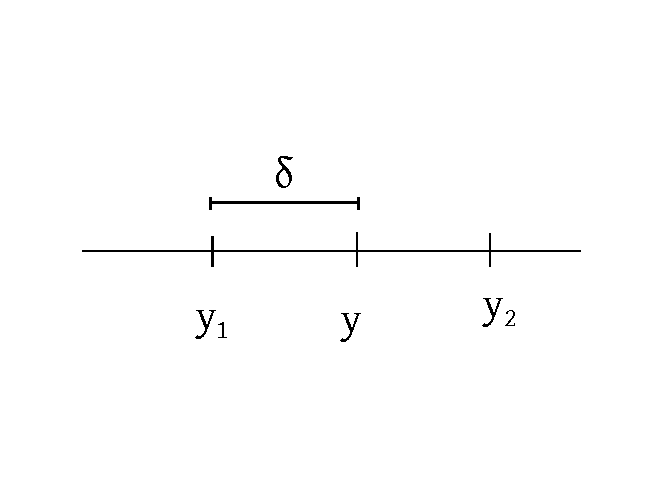
\includegraphics{img/24_setup_delta.pdf}
      \caption{$\delta$, $y$, $y_1$ and $y_2$}
      \label{img:dyyy}
    \end{center}
  \end{figure}

  Choose $\delta = \min\set{y - y_1, y_2 - y} > 0$ (compare with Figure~\ref{img:dyyy}).
  Hence $(y - \delta, y + \delta) \subseteq (y_1, y_2) \forall \eta \in (y - \delta, y + \delta)$,
  \[ f^{-1}(\eta) < f^{-1}(y + \delta) < f^{-1}(y_2) = x_2 = x + \hat\varepsilon \]
  \[ f^{-1}(\eta) < f^{-1}(y - \delta) < f^{-1}(y_1) = x_1 = x - \hat\varepsilon \]
  So $f^{-1}(\eta) \in (x - \hat{\varepsilon}, x + \hat{\varepsilon})$, and accordingly
  \[ \card{\eta - y} < \delta \implies \card{f^{-1}(\eta) - \underbrace{f^{-1}(y)}_{=x}} < c \leq \frac{\varepsilon}{2} < \varepsilon \]
  So $f^{-1}$ is continuous in $y$ and $f^{-1}$ is continuous in $y_0$ analogously.
\end{proof}

Consider
\begin{align*}
  \int_0^b f^{-1}(y) \, dy
    &= \begin{vmatrix}
      y &= f(x) \\
      dy &= f'(x) \, dx \\
      y = 0 &\implies x = f^{-1}(0) = 0 \\
      y = b &\implies x = f^{-1}(b)
    \end{vmatrix} \\
    &= \int_0^{f^{-1}(b)} \underbrace{f^{-1}(f(x))}_{=x} \cdot f'(x) \, dx = \int_0^{f^{-1}(b)} x \cdot f'(x) \, dx \\
    &\underbrace{=}_{\text{integration by parts}} \left. x \cdot f(x) \right|_0^{f^{-1}(b)} - 0 \int_0^{f^{-1}(b)} 1 \cdot f(x) \, dx \\
    &= f^{-1}(b) \cdot b - \int_0^{f^{-1}(b)} f(x) \, dx
\end{align*}
So
\[
  I \coloneqq \int_0^a f(x) \, dx + \int_0^b f^{-1}(y) \, dy = \int_{f^{-1}(b)}^0 f(x) \, dx + b \cdot f^{-1}(b)
\] \[
  = \int_{f^{-1}(b)}^a f(x) \, dx + b \cdot f^{-1}(b)
\]

\begin{description}
  \item[Case 1] $a = f^{-1}(b)$
    \[ \implies I = \underbrace{\int_a^a f(x) \, dx}_{=0} + b \cdot a \]
  \item[Case 2] $b < f(a)$, and accordingly $f^{-1}(b) < a$
    \[ \implies \int_{f^{-1}(b)}^a \underbrace{f(x)}_{f(f^{-1}(b)) \text{ for } x > f^{-1}(b)} \, dx > \overbrace{b}^{\text{minimal value}} \cdot \underbrace{(a - f^{-1}(b))}_{\text{length of integration interval}}  \]
    Therefore $I > b(a - f^{-1}(b)) + b \cdot f^{-1}(b) = ab$.
  \item[Case 3] $b > f(a)$, and accordingly $f^{-1}(b) > a$
    \[ \int_{f^{-1}(b)}^a f(x) \, dx = \int_a^{f^{-1}(b)} \underbrace{(-f(x))}_{\substack{\text{monotonically decreasing} \\ > -f(f^{-1}(b)) \forall x \in [a,f^{-1}(b))}} \, dx > -f(f^{-1}(b)) \cdot (f^{-1}(b) - a) \]
    \[ = -b(f^{-1}(b) - a) \]
    \[ I > -b (f^{-1}(b) - a) + b \cdot f^{-1}(b) = ab \]
\end{description}

\begin{remark}
  Young's inequality also holds without requiring differentiability of $f$ (but the proof is more complex).
\end{remark}

\index{Conjugate exponents}
\begin{lemma}[Special case of Young's inequality] % Lemma 14
  \label{lemma14}
  Let $A, B \geq 0$ and $p,q > 1$ such that $\frac1p + \frac1q = 1 \iff p + q = p \cdot q$.
  Then $p$ and $q$ are called \emph{conjugate exponents}.
  Then $AB \leq \frac{A^p}{p} + \frac{B^q}{q}$.
\end{lemma}
\begin{proof}
  \[ f(x) = x^{p-1} \text{ in Young's inequality} \]
  \[ y = x^{p-1} \iff x = y^{\frac{1}{p-1}} \]
  \[ \frac{1}{p-1} = q - 1 \text{ is immediate, because } \]
  \[ \frac{1}{p-1} = q - 1 \iff 1 = pq - p - q + 1 \iff p + q = pq \]
  So $f^{-1}(y) = y^{\frac{1}{p-1}} = y^{q - 1}$.
  By Young's inequality:
  \[ AB \leq \int_0^A x^{p-1} \, dx + \int_0^B y^{q - 1} \, dy \]
  \[ = \left.\frac{x^p}{p}\right|_0^A + \left. \frac{y^q}{q} \right|_0^B = \frac{A^p}{p} + \frac{B^q}{q} \]
\end{proof}

\begin{remark}
  \[ AB = \frac{A^p}{p} + \frac{B^q}{q} \]
  Equality holds if and only if $B = A^{p-1} \iff B^q = A^{\overbrace{pq-q}^{p}} = A^p$.
\end{remark}

\subsection{H\"older's ineqaulity}

\index{H\"older's inequality}
\index{$L^p$-norm}
\begin{theorem}[H\"older's inequality] % Satz 10
  Let $I$ be an interval with boundary values $a$ and $b$. $-\infty \leq a < b \leq +\infty$.
  Let $p$ and $q$ be conjugate exponents. Let $f_1$ and $f_2$ be regulated function on $I$
  such that
  \[ \int_a^b \card{f_1(x)}^p \, dx < \infty \]
  \[ \int_a^b \card{f_2(x)}^q \, dx < \infty \]
  both exist.

  We let $\norm{f_1}_p \coloneqq \left(\int_a^b \card{f_1(x)}^p \, dx\right)^{\frac1p}$ and $\norm{f_2}_q \coloneqq \left(\int_a^b \card{f_2(x)}^q \, dx\right)^{\frac1q}$.
  They are called $L^p$-norm of $f_1$ and $L^q$-norm of $f_2$.

  Then
  \[ \int_a^b \card{f_1(x) \cdot f_2(x)} \, dx < \infty \]
  exists and
  \[ \int_a^b \card{f_1(x) \cdot f_2(x)} \, dx \leq \norm{f_1}_p \cdot \norm{f_2}_q \]
\end{theorem}

\begin{proof}
  Assume that $\norm{f_1}_p > 0$  and $\norm{f_2}_q > 0$.
  Let $A = \frac{\card{f_1(x)}}{\norm{f_1}_p}$ and $B = \frac{\card{f_2(x)}}{\norm{f_2}_q}$.
  By Lemma~\ref{lemma14},
  \[
    \frac{\card{f_1(x)}}{\norm{f_1}_p} \cdot \frac{\card{f_2(x)}}{\norm{f_2}_q}
    \leq \frac{1}{q} \cdot \frac{\card{f_1(x)}^p}{\norm{f_1}^p_p} + \frac1q \cdot \frac{\card{f_2(x)}^q}{\norm{f_2}_q^q}
  \]
  We integrate the inequality,
  \[
    \frac{1}{\norm{f_1}_p \cdot \norm{f_2}_q} \cdot \int_a^b \card{f_1(x) \cdot f_2(x)} \, dx
  \] \[
    \leq \frac{1}{p} \cdot \frac{1}{\norm{f_1}^p_p} \cdot \underbrace{\int_a^b \card{f_1(x)^p} \, dx}_{= \norm{f_1}_1^p}
    + \frac1q \cdot \frac{1}{\norm{f_2}_q^q} \underbrace{\int_a^b \card{f_2(x)}^q \, dx}_{= \norm{f_2}_q^q}
    = \frac1p + \frac1q = 1
  \]

  \[
    \frac{1}{\norm{f_1}_p \cdot \norm{f_2}_q} \cdot \int_a^b \card{f_1(x) \cdot f_2(x)} \, dx
    \implies \int_a^b \card{f_1(x) f_2(x)} \, dx
    \leq \norm{f_1}_p \cdot \norm{f_2}_q
  \]
  Special case: Let $\norm{f_1}_p = 0$
  \[
    \implies
    \left(\int_a^b \card{f_1(x)}^p \, dx\right)^{\frac1p} = 0
    \implies \int_a^b \underbrace{\card{f_1(x)}^p}_{\geq 0} \, dx = 0
  \]
  By Theorem~\ref{satz7countable}, $f_1(x) = 0 \forall x \in [a,b] \setminus A$
  and $A$ is at most countable.
  \[ \implies f_1(x) \cdot f_2(x) = 0 \forall x \in [a,b] \setminus A \]
  \[ \implies \int_a^b \card{f_1(x) \cdot f_2(x)} \, dx = 0 \]
  \[ \implies 0 = 0 \text{ in H\"older's inequality} \]
\end{proof}

\index{Cauchy-Schwarz inequality}
\begin{remark}[Special case of H\"older's inequality]
  Let $p = q = 2$, $\frac12 + \frac12 = 1$.
  \[ \int_a^b \card{f_1(x) \cdot f_2(x)} \, dx \leq \norm{f_1}_2 \norm{f_2}_2 \]
  is called Cauchy-Schwarz inequality for $L^2$ functions.

  \[ \int_a^b f_1(x) f_2(x) \, dx = \angel{f_1,f_2}_2 = \angel{f_1, f_2}_{L^2} \]
  is an inner product on a proper space of functions.
\end{remark}

\section{Elaboration on differential calculus}

We consider a metric space $X$ and functions $f: X \to \mathbb C$.
We define a concept of uniform convergence of such sequences:
\[ f_n: X \to \mathbb C \quad (n \in \mathbb N) \text{ and } f: X \to \mathbb C \]
We say, $(f_n)_{n \in \mathbb N}$ converges uniformly towards $f$ if $\forall \varepsilon > 0 \forall N \in \mathbb N$
such that $\forall x \in X$ and $\forall n \geq N$
\[ \underbrace{\card{f_n(x) - f(x)}}_{\text{absolute value in } \mathbb C} < \varepsilon \]
\[ \iff \sup\set{\card{f_n(x) - f(x)}: x \in X} < \varepsilon \]

\begin{remark}
  Do not use $\norm{f}_{\infty}$ for the definition of uniform convergence,
  because $f_n$ and $f$ must not be necessarily bounded. Hence,
  \[ \norm{f}_\infty = \set{\card{f(x)}: x \in X} \]
  must not be finite.
\end{remark}

\begin{theorem} % Satz 1
  \label{satz1cont}
  Let $X$ be a metric space, $f_n: X \to \mathbb C$ be a sequence of continuous functions and $f: X \to \mathbb C$ such that
  $f_n \to f$ uniform on $X$. Then $f$ is also continuous on $X$.
\end{theorem}

\dateref{2018/05/03}

\begin{proof}
  Let $\varepsilon > 0$ be arbitrary.
  Choose $x \in X$. Show: $f$ is continuous in $x$.

  Compare with Figure~\ref{img:uniconv}.

  \begin{figure}[t]
    \begin{center}
      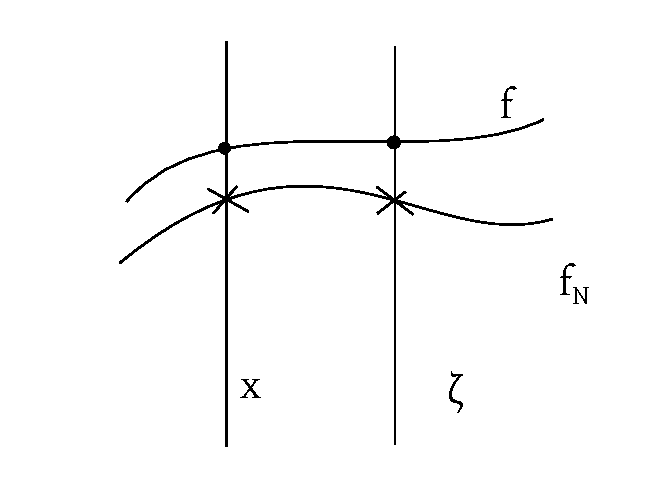
\includegraphics{img/25_uniform_convergence_of_fN_to_f.pdf}
      \caption{Uniform convergence of $f_N$ to $f$}
      \label{img:uniconv}
    \end{center}
  \end{figure}

  Because of uniform convergence $f_n \to f$, there exists $N \in \mathbb N$ such that $\card{f_N(z) - f(z)} < \frac\varepsilon3 \forall z \in X$.
  Let $N$ be fixed. Because $f_N$ is continuous in $x$, there exists $\delta > 0$ such that $d(x, \xi) < \delta \implies \card{f_N(\xi) - f_N(x)} < \frac\varepsilon3$.

  We consider now $\xi \in X$ with $d_X(x, \xi) < \delta$. Then
  \begin{align*}
    \card{f(x) - f(\xi)}
      &= \card{f(x) - f_N(x) + f_N(x) - f_N(\xi) + f_N(\xi) - f(\xi)} \\
      &\leq \underbrace{\card{f(n) - f_N(x)}}_{< \frac\varepsilon2} + \underbrace{\card{f_N(x) - f_N(\xi)}}_{< \frac\varepsilon3} + \underbrace{\card{f_N(\xi) - f(\xi)}}_{< \frac\varepsilon3} \\
      &= \varepsilon
  \end{align*}
  by uniform convergence, by continuity and by uniform convergence respectively.

  Thus, $f$ is continuous in $x$.
\end{proof}

\begin{theorem} % Satz 2
  Let $P(z) = \sum_{k=0}^\infty a_k z^k$ be a power series in $\mathbb C$ with convergence radius $\rho_P > 0$.
  Furthermore, let $0 < r < \rho_P$.
  Let $P_n(z) = \sum_{k=0}^n a_k z^k$ ($n$-th partial sum of $P$).
  Then $P_n \to P$ uniformly on $\overline{K_r(0)}$.
\end{theorem}

\begin{remark}
  \begin{figure}[t]
    \begin{center}
      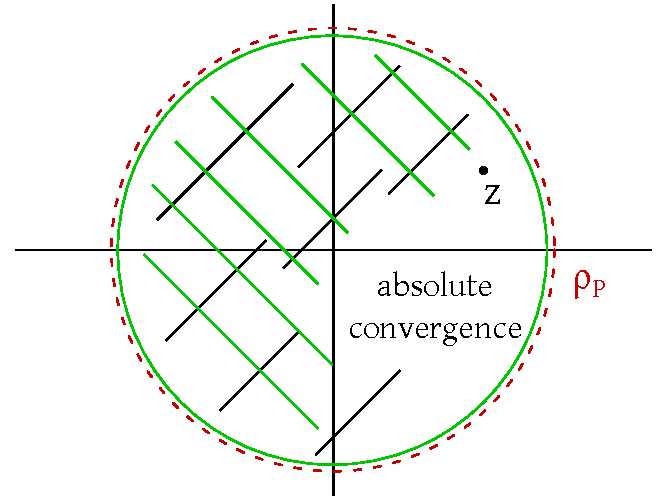
\includegraphics{img/26_uniform_convergence.pdf}
      \caption{We cannot make a general statement about convergence/divergence. But on every small closed sphere $P$ converges absolutely for every $z$}
      \label{img:uconv}
    \end{center}
  \end{figure}
\end{remark}

\begin{proof}
  Approximation theorem for power series.
  Lettl Analysis 1, lecture notes, section 5, theorem~10.

  Let $0 < r < \rho_P$. Choose $\overline{r}$ with $r < \overline{r} < \rho_P$.
  Then it holds for $z \in \overline{K_r(0)}$ that
  \[ \card{P(z) - P_n(z)} < \frac{\overline{r}}{\overline{r} - r} \cdot \left(\frac{r}{\overline{r}}\right)^n \]
  \[ \frac{r}{\overline{r}} < 1 \]
  hence $\left(\frac{r}{\overline{r}}\right)^n$ is arbitrary small, for every $n$ sufficiently large.
  \[ \implies \sup\set{\card{P(z) - P_n(z): z \in \overline{K_r(0)}}} \leq \underbrace{\frac{\overline r}{\overline r - r}}_{\text{fixed}} \cdot \underbrace{\left(\frac{r}{\overline{r}}\right)^n}_{\substack{\text{arbitrary small for $n$} \\ \text{sufficiently large}}} \]
  Hence, $P_n \to P$ uniform on $\overline{K_r(0)}$.
\end{proof}

\begin{corollary}
  $P$ is continuous on $K_{\rho_P}(0)$.
\end{corollary}

\begin{theorem}
  Let $I \subseteq \mathbb R$ be an interval.
  Let $f_n: I \to \mathbb R$ be continuously differentiable on $I \forall n \in \mathbb N$.
  \begin{enumerate}
    \item $\exists g: I \to \mathbb R$ such that $f_n' \to g$ uniform on $I$
    \item $\exists f: I \to \mathbb R$ such that $\forall x \in I: f(x) = \lim_{n\to\infty} f_n(x)$ (\enquote{pointwise convergence}).
  \end{enumerate}
  Then $f$ is continuously differentiable on $I$ and $g = f'$.
\end{theorem}

\begin{proof}
  $g$ is continuous as uniform limit of continuous $f_n'$ (Theorem~\ref{satz1cont}).
  For $f_n$, the Fundamental Theorem of Differential Calculus can be applied ($f_n'$ is continuous, hence a regulated function).
  Let $x_0 \in I$. Then
  \[ f_n(x) = f_n(x_0) + \int_{x_0}^x f_n'(\xi) \, d\xi \]
  Convergence for $n \to \infty$:
  \[ f_n(x) \to f(x) \qquad f_n(x_0) \to f(x_0) \]
  (Pointwise convergence)
  \[ \int_{x_0}^x f_n'(\xi) \, d\xi \to \int_{x_0}^x g(\xi) \, d\xi \]
  Therefore, for $n \to \infty$,
  \[ f(x) = f(x_0) + \int^x_{x_0} g(\xi) \, d\xi \]
  The right-hand side is continuously differentiable by $x$ according to the Fundamental Theorem, variant 1,
  with
  \[ \left(f(x_0) + \int_{x_0}^x g(\xi) \, d\xi\right)'(x) = g(x) \]
  Hence, by $f(x) = f(x_0) + \int^x_{x_0} g(\xi) \, d\xi$ it follows that
  \[ f'(x) = g(x) \qquad \forall x \in I \]
\end{proof}

To finish our proof, we need a result we missed in the section about Integrals.

\begin{lemma}
  Let $(f_n)_{n \in \mathbb N}$ be a sequence of regulated functions on $[a,b]$ and
  $f_n \to f$ uniform on $[a,b]$. Then
  \[ \int_a^b \card{f_n - f} \, dx \to 0 \qquad \text{ for } n \to \infty \qquad \text{ especially } \int_a^b f_n \, dx \to \int_a^b f \, dx \]
\end{lemma}

\begin{proof}
  $f$ as a uniform limit of regulated functions is a regulated function.
  The proof has been done in the practicals.

  Let $N \in \mathbb N$ large enough such that
  \[ \forall n \geq N \forall x \in [a,b]: \card{f_n(x) - f(x)} < \frac{\varepsilon}{b - a} \]
  Then
  \[ \int_a^b \card{f_n(x) - f(x)} \, dx < \int_a^b \frac{\varepsilon}{b - a} \, dx = \frac{\varepsilon}{b - a} (b - a) = \varepsilon \]
  Hence,
  \[ \lim_{n\to\infty} \int_a^b \card{f_n(x) - f(x)} \, dx = 0 \]
  \[ \underbrace{\card{\int_a^b f_n \, dx - \int_a^b f \, dx}}_{\implies \to 0 } \leq \underbrace{\int_a^b \card{f_n - f} \, dx}_{\to 0} \]
  So,
  \[ \int_a^b f \, dx = \lim_{n\to\infty} \int_a^b f_n \, dx \]
\end{proof}

\subsection{Higher derivatives and Taylor's Theorem}

\begin{definition} % Definition 1
  Let $f: I \to \mathbb R$. $I \subseteq \mathbb R$ is an interval.
  We define inductively:
  \[ f^{(0)}(x) = f(x) \]
  Assume $f^{(n-1)}$ is defined continuously on $I$ and differentiable in $x \in I$.
  Then we let
  \[ f^{(n)}(x) = \left(f^{(n-1)}\right)'(x) \]
  $f^{(n)}(x)$ is called $n$-th derivative of $f$ in $x$.
  
  Notational remark:
  \[ f^{(0)} = f \qquad f^{(1)} = f' \qquad f^{(2)} = f'' \qquad f^{(3)} = f''' \qquad f^{(4)} = f'''' \]

  Furthermore, we let
  \[ \mathcal C^n(I) \coloneqq \set{f: I \to \mathbb R: f^{(k)}(x) \text{ exists } \forall x \in I \text{ and } x \mapsto f^{(k)}(x) \text{ is continuous } \forall 0 \leq k \leq n} \]
  We call $\mathcal C$ the space of $n$-times continuously differentiable functions on $I$.
\end{definition}

\begin{remark}
  $\mathcal C^n(I)$ is a vector space.
  If $I = [a,b]$ is compact, then
  \[ \norm{f}_{\mathcal C^n} = \max\set{\sup{\card{f^{(k)}(x)}: x \in I}: 0 \leq k \leq n} \]
  defines a norm on $\mathcal C^n(I)$ with $\sup{\card{f^{(k)}(x)}: x \in I} = {\norm{f^{(k)}}_{\infty}}$.
\end{remark}

\begin{remark}[New topic]
  Let $f \in \mathcal C^n(I)$ and $x_0 \in I$. Find an appropriate polynomial $T$ which approximated $f$ in a neighborhood of $x_0$ in the \enquote{best} way.
\end{remark}

\begin{definition} % Definition 2
  Let $P(x) = \sum_{k=0}^n a_k x^k$ be a polynomial with $a_n \neq 0$
  (hence degree of $P$ is $n$).
  \[ P \in \mathbb R[x] \dots \text{ set of all polynomials with coefficients in } \mathbb R \]
  This set of polynomials is a ring.

  $x_0 \in \mathbb R$ is called $k$-times root of $P$ ($k \in \mathbb N$) if $Q \in \mathbb R[x]$ exists such that
  $P(x) = (x - x_0)^k Q(x)$ with $Q(x_0) \neq 0$.
\end{definition}

\begin{remark}
  $P(x) = (x - x_0)^k \cdot Q(x)$ means that division of $P$ by $(x - x_0)^k$ gives no remainder.
  Recall that division with remainder means that $\exists \hat Q, \hat R$ that are polynomials of degree $\hat R < k$,
  \[ P(x) = (x - x_0)^k \cdot \hat Q(x) + \hat R(x) \]
  $\hat Q, \hat R$ is unique.
  If $P(x) = (x - x_0)^k \cdot Q(x) \implies \hat R = 0, \hat Q = Q$.
\end{remark}

\begin{lemma} % Lemma 2
  \label{lemma2-2}
  Let $P(x) = \sum_{l=0}^n a_l x^l$ with $a_n \neq 0$.
  Let $1 \leq k \leq n$. Then $x_0 \in \mathbb R$ is a $k$-times root of polynomial $P \iff$
  $P^{(j)}(x_0) = 0$ for $j = 0, \ldots, k-1$ and $P^{(k)}(x_0) \neq 0$.
\end{lemma}

\begin{proof}
  Proof by complete induction.

  \begin{description}
    \item[Induction begin]
      Consider $k=1$. Direction $\implies$.

      Let $x_0$ be a simple root of $P$, then $P(x) = (x - x_0) \cdot Q(x)$ and $Q(x_0) \neq 0$.
      Hence, $P(x_0) = (x_0 - x_0) \cdot Q(x_0) = 0$ and $P'(x) = Q(x) + (x - x_0) \cdot Q'(x)$.
      Thus, $P'(x_0) = Q(x_0) + (x_0 - x_0) \cdot Q'(x_0) = Q(x_0) \neq 0$.

      Direction $\impliedby$.

      Let $P(x_0) = 0$ and $P'(x_0) \neq 0$. Division with remainder: $P(x) = (x - x_0) \cdot Q(x) + R(x)$
      with $\operatorname{degree}(R) \leq \operatorname{degree}(x - x_0) = 1$. Thus, $R$ is constant.
      We insert $x_0$. This gives $P(x_0) = (x_0 - x_0) \cdot Q(x_0) + R$ with $P(x_0) = 0$ and $(x_0 - x_0) = 0$.
      Hence, $R = 0$ is the zero polynomial and $P(x) = (x - x_0) \cdot Q(x)$.
      It remains to show that $Q(x_0) \neq 0$. $P'(x) = 1\cdot Q(x_0) + (x - x_0) \cdot Q'(x_0)$.
      We insert $x = x_0 \implies 0 \neq P'(x_0) = Q(x_0) + (x_0 - x_0) \cdot Q'(x)$.
      Thus is holds that $Q(x_0) = P'(x_0) \neq 0$.
    \item[Induction step] $k \to k+1$ \hfill{}
      \begin{claim}[Auxiliary claim]
        Let $P(x) = (x - x_0) \cdot \tilde P(x)$.
        Let $P, \tilde P$ be polynomials. Then it holds $\forall j \in \mathbb N$ that
        \[ P^{(j)}(x) = (x - x_0) \cdot \tilde P^{(j)}(x) + j \cdot \tilde P^{(j-1)}(x) \]
      \end{claim}
      \begin{proof}
        Proof by complete induction.

        Let $j = 1$.
        \[ P'(x) = 1 \cdot \underbrace{\tilde P(x)}_{\tilde P^{(0)}(x)} + (x - x_0) \cdot \underbrace{\tilde P'(x)}_{\tilde P^{(1)}(x)} \]

        Consider $j \to j + 1$.
        \begin{align*}
          P^{(j+1)}(x) &= \left(P^{(j)}\right)'(x) \\
          &\underbrace{=}_{\substack{\text{induction} \\ \text{assumption}}} ((x - x_0) \cdot \tilde P^{(j)}(x) \\
          &+ j \tilde P^{(j-1)}(x))' (x - x_0) \tilde P^{(j+1)}(x) + \tilde P^{(j)}(x) + j \cdot \tilde P^{(j)}(x) \\
          &= (x - x_0) \tilde P^{(j+1)}(x) + (j + 1) \cdot \tilde P^{j}(x)
        \end{align*}
      \end{proof}

      We continue with the induction step after verifying our auxiliary claim. Direction $\implies$.

      Let $x_0$ be an $k+1$ times zero of $P$. Hence $P(x) = (x - x_0)^{k+1} \cdot Q(x)$. $Q(x_0) \neq 0$.
      Let $\tilde P(x) = (x - x_0)^k \cdot Q(x)$. 
      We can apply the induction assumption on $\tilde P$. Hence
      \[ \tilde P^{(j)} = 0 \qquad \text{ for } j = 0, \ldots, k-1 \qquad \text{ and } \qquad \tilde P^{(k)}(x_0) \neq 0 \]
      \[ P(x) = (x - x_0) \cdot \tilde P(x) \]
      By the auxiliary claim, $P^{(j)}(x) = (x - x_0) \cdot \tilde P^{(j)}(x) + j \cdot \tilde P^{(j-1)}(x)$.
      Therefore
      \[
        P^{(j)}(x_0) = j \cdot \tilde P^{(j-1)}(x) = \begin{cases}
          0 & \text{ for } j = 0, \dots, k \\
          (k+1)\tilde P^{(k)}(x_0) \neq 0 & \text{ for } j = k+1
        \end{cases}
      \]
      Hence, our claim about the derivatives is true (all derivatives are zero).

      Direction $\impliedby$.

      Let $P^{(j)}(x_0) = 0$ for $j = 0, \dots, k$ and $P^{(k+1)}(x_0) \neq 0$ and induction assumption holds for $k$.
      Division with remainder and $P^{(0)}(x_0) = 0 \implies P(x) = (x - x_0) \cdot \tilde P(x)$.
      By our auxiliary claim, we get
      \[ P^{(j)}(x) = (x - x_0) \cdot \tilde P^{(j)}(x) + j \tilde P^{(j-1)}(x) \]
      we insert $x = x_0$ and use $P^{(j)}(x_0) = 0$ for $j = 0, \dots, k$
      \[ \implies \tilde P^{(j)}(x_0) = 0 \qquad \text{ for } j = 0, \dots, k-1 \]
      By the induction assumption, $\tilde P(x) = (x - x_0)^k Q(x)$ with $Q(x_0) \neq 0$
      \[ \implies P(x) = (x - x_0) \cdot \tilde P(x) = (x - x_0)^{k+1} Q(x) \]
  \end{description}
\end{proof}

\dateref{2018/05/08}

\index{Taylor polynomial of $f$ of order $n$ in $x_0$}
\begin{definition} % Definition 3
  \label{def3}
  Let $I \subseteq \mathbb R$ be an interval, $f \in \mathcal C^n(I)$.
  We let
  \[ T_f^n(x; x_0) = \sum_{k=0}^n \frac{1}{k!} f^{(k)}(x_0) (x - x_0)^k \]

  $T_f^n(x; x_0)$ is a polynomial in $x$ with $\operatorname{degree}(T_f^n) \leq n$.
  $T_f^n(x; x_0)$ is called \emph{Taylor polynomial of $f$ of order $n$ in $x_0$}.
\end{definition}

Brook Taylor (1685--1731)

\begin{lemma} % Lemma 3
  The premise is the same like in Definition~\ref{def3}.
  The Taylor polynomial of $T_f^n(x; x_0)$ is the only polynomial of degree $\neq n$ which satisfies
  \[ (T_f^n)^{(k)}(x_0) = f^{(k)}(x_0) \qquad \text{ for k = 0, \dots, n} \]
\end{lemma}

\begin{proof}
  Claim:
  \[ (T_f^n)^{(k)}(x; x_0) = \sum_{l=k}^n \frac{f^{(l)}(x_0)}{(l - k)!} (x - x_0)^{l-k} \qquad \text{ for } 0 \leq k \leq n \]

  Proof of the claim by complete induction:
  \begin{description}
    \item[Induction base $n = 0$] 
      \[ (T_f^n)^{(0)} (x; x_0) = \sum_{l=0}^n \frac{f^{(l)}(x_0)}{l!} (x - x_0)^l \]
    \item[Induction step $k \to k + 1$]
      Let $(T_f^n)^{(k)}(x; x_0)$
      \[ = \sum_{l=k}^{n} \frac{f^{(l)}(x_0)}{(l - k)!} (x - x_0)^{(l-k)} \]
      by induction hypothesis. Then,
      \begin{align*}
        &= \sum_{l=k+1}^n \frac{f^{(l)}(x_0)}{(l-k)!} (l - k) \cdot (x - x_0)^{l - k - 1} \\
        &= \sum_{l=k+1}^n \frac{f^{(l)}(x_0)}{(l - (k+1))!} (x - x_0)^{l - (k+1)}
      \end{align*}
      We apply insertion: $x = x_0$ into $(T_f^n)^{(k)}(x; x_0)$
      \[ (T_f^n)^{(k)}(x; x_0) = \sum_{l=k}^n \frac{f^{(l)}(x_0)}{(l - k)!} (x - x_0)^{l-k} = \frac{f^{(k)}(x_0)}{0!} = f^{(k)}(x_0) \]
  \end{description}

  We need to prove uniqueness: Let $T, \tilde T$ be polynomials with $T^{(k)}(x_0) = \tilde T^{(k)}(x_0) = f^{(k)}(x_0)$ for $k = 0, \dots, n$.
  Assume $T \neq \tilde T$, hence $T - \tilde T \neq 0$ (where $0$ is the zero polynomial).
  For $P = T - \tilde T$,
  \[ P^{(k)}(x_0) = T^{(k)}(x_0) - \tilde T^{(k)}(x_0) = 0 \qquad (\text{for } 0 \leq k \leq n) \]
  By Lemma~\ref{lemma2-2}, $x_0$ is an $n+1$-times root of $P$. Thus, there exists a polynomial $Q \neq 0$ with $Q(x_0) \neq 0$ such that
  \[ \underbrace{P(x)}_{\text{degree } \leq n} = \underbrace{(x - x_0)^{(n+1)} \cdot Q(x)}_{\text{degree } \geq n+1} \]
  This is a contradiction. Hence, $T - \tilde T = 0$.
\end{proof}

\index{Approximation error of a Taylor polynomial}
\index{Remainder of a Taylor polynomial}
\begin{definition} % Definition 4
  \label{def4}
  Let $f \in \mathcal C^n(I)$, $x_0 \in I$. Furthermore let $T_f^n(x; x_0)$ be the Taylor polynomial of $n$-th degree of $f$ in $x_0$.
  We let $R_f^n(x; x_0) = f(x) - T_f^n(x; x_0)$. We call $R_f^{n+1}(x; x_0)$ the \emph{approximation error} of the Taylor polynomial.
  Also called \emph{remainder term of $n+1$-th order}. Compare with Figure~\ref{img:taylor-rem}.
\end{definition}

\begin{figure}[t]
  \begin{center}
    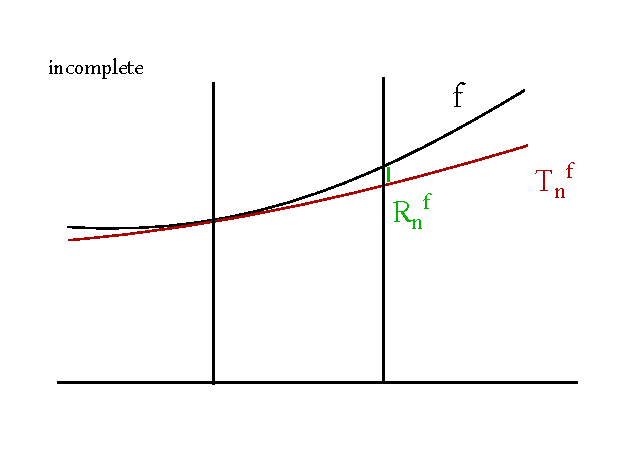
\includegraphics{img/27_taylor_remainder.pdf}
    \caption{Visualization of the remainder term of a Taylor polynomial}
    \label{img:taylor-rem}
  \end{center}
\end{figure}

\index{Integral form of the Taylor remainder}
\begin{theorem} % Satz 4
  \label{thm4} 
  Let $f^{(n+1)}(I)$, $x \in I$, $x_0 \in I$. Then
  \[ R_f^{n+1}(x; x_0) = \frac1{n!} \int_{x_0}^x (x - t)^n f^{(n+1)}(t) \, dt \]
  We call it the \emph{integral form of the remainder term}.
\end{theorem}

\begin{proof}
  Complete induction over $n$.
  \begin{description}
    \item[Induction base $n = 0$]
      \[ T_f^0(x; x_0) = f(x_0) \]
      \begin{align*}
        R_f^1(x; x_0) &= \underbrace{f(x) - f(x_0)}_{f \in \mathcal C^1} \\
          &= \int_{x_0}^x f'(t) \, dt \\
          &= \frac1{0!} \int_{x_0}^x (x - t)^0 f^{(1)}(t) \, dt
      \end{align*}
    \item[Induction step $n-1 \to n$]
      \begin{align*}
        R_f^n(x; x_0) &= f(x) - T_f^{n-1}(x; x_0) \\
          &\underbrace{=}_{\text{ind. hypothesis}} \frac{1}{(n-1)!} \int_{x_0}^x (x - t)^{n-1} f^{(n)}(t) \, dt \\
          &= \begin{vmatrix} u' = (x - t)^{n-1} & v = f^{(n)}(t) \\ u = -\frac1n (x - t)^n & v' = f^{(n+1)}(t) \end{vmatrix} \\
          &= \left.\frac{1}{(n-1)!} \underbrace{\left[-\frac1n (x - t)^n \cdot f^{(n)}(t)\right]}_{= \frac1{n!} (x - x_0)^n \cdot f^{(n)}(x_0)} \right|_{t = x_0}^{x} \\
          &+ \underbrace{\frac{1}{(n-1)!} \int \frac1n (x - t)^n \cdot f^{(n+1)}(t) \, dt}_{= \frac1{n!} \int_{x_0}^x (x - t)^n \cdot f^{(n+1)}(t) \, dt}
      \end{align*}
      So,
      \[ f(x) \underbrace{- T_f^{n-1}(x; x_0) - \frac{1}{n!} f^{(n)}(x_0)(x - x_0)^n}_{- T_f^n(x; x_0)} \]
      \[ = \frac1{n!} \int_{x_0}^x (x - t)^n \cdot f^{(n+1)}(t) \, dt \]
      Therefore,
      \[ R_f^{(n+1)}(x; x_0) = \frac{1}{n!} \int_{x_0}^x (x - t)^n f^{(n+1)}(t) \, dt \]
  \end{description}
\end{proof}

\index{Lagrange form of the remainder}
\begin{theorem}[Lagrange form of the remainder term] % Satz 5
  \label{thm5}
  Let $f \in \mathcal C^{n+1}(I)$, $n \in \mathbb N_0$, $x, x_0 \in I$, $x \neq x_0$.
  Then there exists some $\xi$ between $x_0$ and $x$ (hence, $\xi \in (x_0, x)$ if $x > x_0$ or $\xi \in (x, x_0)$ if $x < x_0$) such that
  \[ R_f^{(n+1)}(x; x_0) = \frac{1}{(n+1)!} f^{(n+1)}(\xi) (x - x_0)^{n+1} \]
\end{theorem}

\begin{proof}
  Idea: we apply the Mean Value Theorem for definite integrals on the Taylor remainder.

  \begin{description}
    \item[Case 1] Let $x_0 < x$.
      \begin{align*}
        R_f^{n+1}(x; x_0)
          &= \frac{1}{n!} \int_{x_0}^x \underbrace{(x - t)^n}_{\substack{\geq 0 \\ \text{regulated function}}} \underbrace{f^{(n+1)}(t)}_{\text{continuous in } t} \, dt \\
          &\underbrace{=}_{\text{MVT}} \frac{1}{n!} f^{(n+1)}(\xi) \cdot \int_{x_0}^x (x - t)^n \, dt \\
          &= \frac{1}{n!} f^{(n+1)} (\xi) \left[- \frac{1}{n+1} (x - t)^{n+1}\right]_{t = x_0}^x \\
          &= \frac{1}{(n+1)!} f^{(n+1)}(\xi)(x - x_0)^{n+1}
      \end{align*}
      where MVT is the Mean Value Theorem for definite integrals (Theorem~\ref{satz3}).
    \item[Case 2] Let $x < x_0$ and $n$ odd.
      \begin{align*}
        R_f^{n+1}(x; x_0) &= -\frac{1}{n!} \int_{x}^{x_0} \underbrace{(x - t)^n}_{= (-1)^n (t - x)^n} \cdot f^{(n+1)}(t) \, dt \\
          &= \frac{1}{n!} \int_x^{x_0} \underbrace{(t - x)^n}_{\geq 0} \cdot \underbrace{f^{(n+1)}(t)}_{\text{continuous}} \, dt \\
          &= \frac{f^{(n+1)}(\xi)}{n!} \int_x^{x_0} (t - x)^n \, dt \\
          &= \left.\frac{f^{(n+1)}(\xi)}{n!} \left[\frac{1}{n+1} (t - x)^{n+1}\right]\right|_{x}^{x_0} \\
          &= \frac{1}{(n+1)!} f^{(n+1)}(\xi)(x_0 - x)^{n+1} \\
        \intertext{$n+1$ is even} \\
          &= \frac{1}{(n+1)!} f^{(n+1)}(\xi)(x - x_0)^{n+1}
      \end{align*}
    \item[Case 3] Let $x < x_0$ and $n$ even.
      \begin{align*}
        R_f^{n+1}(x; x)
          &= -\frac{1}{n!} \int_x^{x_0} \underbrace{(x - t)^n}_{\geq 0} \cdot \underbrace{f^{(n+1)}(t)}_{\text{continuous}} \, dt \\
          &= -\frac1{n!} f^{(n+1)}(\xi) \cdot \int_x^{x_0} (x - t)^n \, dt \\
          &= \left. -\frac1{n!} f^{(n+1)}(\xi) \cdot \left[-\frac{1}{n+1} (x - t)^{n+1}\right]\right|_x^{x_0} \\
          &= \frac{1}{(n+1)!} f^{(n+1)}(\xi) (x - x_0)^{n+1}
      \end{align*}
  \end{description}
\end{proof}

Any extreme value satisfies that its derivative is zero. But not every point with derivative zero is an extreme value.
We now consider conditions to select extreme values from all value satisfying derivative zero.

\begin{corollary}[Sufficient conditions for existence of extreme values]
  Let $I$ be an open interval. Let $x_0 \in I$ and $f \in \mathcal C^{n+1}(I)$. Assume
  \[ f^{(1)}(x_0) = f^{(2)}(x_0) = \dots = f^{(n)}(x_0) = 0 \]
  and $f^{(n+1)}(x_0) \neq 0$. Then $f$ in $x_0$ has
  \begin{enumerate}
    \item a strict local maximum if $n$ is even and $f^{(n+1)}(x_0) < 0$
    \item a strict local minimum if $n$ is odd and $f^{(n+1)}(x_0) > 0$
    \item no extreme value in $x_0$ if $n$ is even.
  \end{enumerate}
\end{corollary}

\begin{proof}
  \begin{description}
    \item[Case a]
      Let $f^{(n+1)}(x_0) < 0$ and $f^{(n+1)}$ be continuous,
      then $\exists \varepsilon > 0$ such that $(x_0 - \varepsilon, x_0 + \varepsilon) \subseteq I$ ($I$ is open)
      and $f^{(n+1)}(\xi) < 0 \forall \xi \in (x_0 - \varepsilon, x_0 + \varepsilon)$.
      Now let $x \in (x_0 - \varepsilon, x_0 + \varepsilon)$.
      Then by Theorem~\ref{thm5},
      \[ \frac{f^{(n+1)}(\xi)}{(n+1)!} (x - x_0)^{n+1} = R_f^{n+1}(x; x_0) = f(x) - \sum_{k=0}^n \frac{1}{k!} f^{(k)}(x_0) (x - x_0)^k = f(x) - f(x_0) \]
      for $k = 1, \dots, n$. So,
      \[ f(x) - f(x_0) = \frac{\overbrace{f^{(n+1)}(\xi)}^{< 0}}{\underbrace{(n+1)!}_{> 0}} \underbrace{(x - x_0)^{\overbrace{n+1}^{\text{even}}}}_{> 0 \text{ for } x \neq x_0} \]
      hence $f(x) - f(x_0) < 0$, and accordingly
      \[ f(x) < f(x_0) \qquad \forall x \in (x_0 - \varepsilon, x_0 + \varepsilon), x \neq x_0 \]
      So $f$ is a strict local maximum.
    \item[Case b] Analogously.
    \item[Case c] We apply the same idea as in Case~a up to the point, where we consider $f(x) - f(x_0)$.
      \[ f(x) - f(x_0) = \frac{f^{(n+1)}(\xi)}{(n+1)!} (x - x_0)^{n+1} \]
      $f^{(n+1)}(\xi)$ has the same sign as $\underbrace{f^{(n+1)}(x_0)}_{\neq 0} \quad \forall \xi \in (x_0 - \varepsilon, x_0 + \varepsilon)$.
      This is feasible due to continuity of $f^{(n+1)}$ for sufficiently small $\varepsilon$.
      \[
        f(x) - f(x_0)
        = \underbrace{\frac{f^{(n+1)}(\xi)}{(n+1)}}_{\text{has constant sign indep. of } x} \cdot {\underbrace{(x - x_0)}_{\text{changes its sign}}}^{\overbrace{n+1}^{\text{odd}}}
      \]
      Therefore $f(x) - f(x_0)$ changes its sign for $x = x_0$. Hence $f$ has no extreme value in $x = x_0$.
  \end{description}
\end{proof}

\index{Qualitative Taylor equation}
\begin{theorem}[Qualitative Taylor equation]
  Let $f \in \mathcal C^n(I)$, $x, x_0 \in I$. Then there exists some function $r \in \mathcal C(I)$ with $r(x_0) = 0$ such that
  \[ f(x) = T_f^n(x; x_0) + (x - x_0)^n \cdot r(x) \]
  and accordingly,
  \[ R_f^{n+1}(x; x_0) = (x - x_0)^n \cdot r(x) \]
\end{theorem}

\begin{remark}
  For some function $r$ with $\lim_{x\to x_0} r(x) = 0$, we also denote $o(x - x_0)$ instead of $r(x)$.
  This general notation is called Landau's Big-Oh notation.
  \[ f(x) = T_f^n(x; x_0) + (x - x_0)^n \cdot o(x - x_0) \]
\end{remark}

\begin{proof}
  Let $r(x) = \frac{f(x) - T_f^n(x; x_0)}{(x - x_0)^n}$ for $x \neq x_0$ and $r(x_0) \coloneqq 0$.
  Then $f$ is continuous and $T_f^n$ is continuous in every point $x \neq x_0$.
  It remains to show that $r$ is continuous in $x = x_0$.
  \begin{align*}
    r(x) &= \frac{1}{(x - x_0)^n} (\underbrace{f(x) - T_f^{n-1}(x; x_0)}_{R_f^n(x; x_0)} - \frac1{n!} f^{(n)}(x_0)(x - x_0)^n) \\
      &\underbrace{=}_{\text{Lagrange}} \frac{1}{(x - x_0)} \left[ \frac{1}{n!} (x - x_0)^n \cdot f^{(n-1)}(\xi) - \frac{1}{n!} f^{(n)}(x_0)(x - x_0)^n \right] \\
    \intertext{$\xi \in (x_0, x)$} \\
      &= \frac{1}{n!} \left[f^{(n)}(\xi) - f^{(n)}(x_0)\right] \to 0 \text{ for } x \to x_0 \text{ because } f^{(n)} \text{ is continuous} \\
    \intertext{as $x_0 < x < x$, hence $\xi \to x_0$ for $x \to x_0$} 
  \end{align*}
  So $\lim_{x\to x_0} r(x) = 0 = r(x_0)$, so $r$ in $x_0$ is continuous.
\end{proof}

\dateref{2018/05/15}

\subsection{Taylor series}

\index{Taylor series}
Assume $f: I \to \mathbb R$ is infinitely often differentiable on $I$, $x_0 \in I$. Then there exists $T_f^n(x; x_0)$ for arbitrary $n \in \mathbb N$.
\[ T_f(x; x_0) = \sum_{k=0}^\infty \frac{f^{(k)}(x_0)}{k!} (x - x_0)^k \]
$T_f(x; x_0)$ defines the \emph{Taylor series} on $f$ in $x_0$.
Power series in $\xi = x - x_0$.
$T_f$ has a convergence radius,
\[ \rho(T_f) = \left[\limsup_{k\to\infty} \sqrt[k]{\frac{\card{f^{(k)}(x_0)}}{k!}}\right]^{-1} \]
If $\rho(T_f) > 0$, then
\[ f(x) = T_f(x; x_0) = \sum_{k=0}^\infty \frac{f^{(k)}(x)}{k!} (x - x_0)^k \]
in $(x_0 - \rho(T_f), x_0 + \rho(T_f))$?
Compare with Figure~\ref{img:tay}.

\begin{figure}[t]
  \begin{center}
    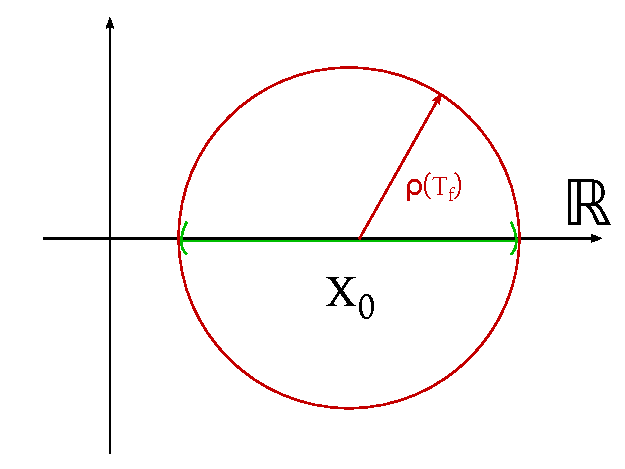
\includegraphics{img/28_Taylor_series.pdf}
    \caption{Taylor series}
    \label{img:tay}
  \end{center}
\end{figure}

\begin{example}[Counterexample]
  Let $f: \mathbb R \to \mathbb R$.
  \[ f(x) = \begin{cases} e^{-\frac1x} & \text{ if } x > 0 \\ 0 & \text{ if } x \leq 0 \end{cases} \]
  It holds for $x > 0$,
  \[ f^{(n)}(x) = \frac{P(x)}{Q(x)} \cdot e^{-\frac1x} \]
  where $P, Q$ are polynomials.
  So the function value (of an infinitely often differentiable function) must not equate with its Taylor series value.
\end{example}

\begin{proof}
  Proof by complete induction over $n$.

  \begin{description}
    \item[Case $n=0$] immediate with $P = Q = 1$.
    \item[Case $n\mapsto n+1$]
      \[ f^{(n+1)}(x) = \left[\underbrace{\frac{P(x)}{Q(x)} \cdot e^{-\frac1x}}_{f^{(n)}(x) \text{ by induction hypothesis}}\right]' \]
      \[ = \frac{P' \cdot Q - Q' \cdot P}{Q^2} \cdot e^{-\frac1x} + \frac PQ \cdot \frac1{x^2} \cdot e^{-\frac1x} \]
      \[ = \frac{(P' Q - Q' P) x^2 + PQ}{Q^2 x^2} \cdot e^{-\frac1x} \]
      It holds that $\lim_{x\to0_+} \frac{P(x)}{Q(x)} \cdot e^{-\frac1x} = 0$.
      Immediately, $\lim_{x \to 0^-} f^{(n)}(x) = 0$, hence $f^{(n)}(0) = 0 \forall n \in \mathbb N$.
      $f$ is arbitrarily often continuously differentiable on $\mathbb R$. Thus,
      \[ T_f(x; 0) = \sum_{k=0}^\infty \frac{\overbrace{f^{(k)}(0)}^{=0}}{k!} x^k = 0 \]
      but $f(x) \neq 0$ on $\mathbb R$. Thus, $f \neq T_f(x; 0)$.
      But $R_f = f - T_f(x; 0) = f$.
      \[ \card{R_f(x)} \leq c_n \card{x}^n \qquad \forall n \in \mathbb N \]
  \end{description}
\end{proof}

\begin{theorem} % Satz 7
  Let $f(x) = \sum_{k=0}^\infty a_k (x - x_0)^k$ be an analytical\footnote{Reminder: A function is analytical if it is locally given by a convergent power series.} function with convergence radius $\rho(f) > 0$.
  Then $f$ is infinitely often continuously differentiable on $I \coloneqq (x_0 - \rho(f), x_0 + \rho(f))$
  and $a_k = \frac{f^{(k)}(x_0)}{k!}$, hence the given power series is the Taylor series of the function.
\end{theorem}

\begin{proof}
  See Analysis 1 lecture notes, chapter 8, theorem 1 by G. Lettl.

  $f$ is differentiable on $I = (x_0 - \rho(f), x_0 + \rho(f))$ and $f'(x) = \sum_{k=0}^\infty k a_k (x - x_0)^{k-1}$.
  Thus, $f'$ is also analytical and the power series of $f'$ converges on $K(x_0) \implies \rho(f') \geq \rho(f)$
  (if you consider the Cauchy-Hadamard Theorem, then $\rho(f') = \rho(f)$).

  Induction:
  $f^{(n)}(x)$ is analytical on $I$ and
  \[ f^{(n)}(x) = \sum_{k=n}^\infty k \cdot (k - 1) \dots (k - n + 1) \cdot a_k \cdot (x - x_0)^{k-n} \]
  We insert: $x = x_0$
  \[ f^{(n)}(x_0) = n \cdot (n - 1) \dots 1 \cdot a_n \implies a_n = \frac{f^{(n)}(x_0)}{n!} \]
\end{proof}

\begin{figure}[t]
  \begin{center}
    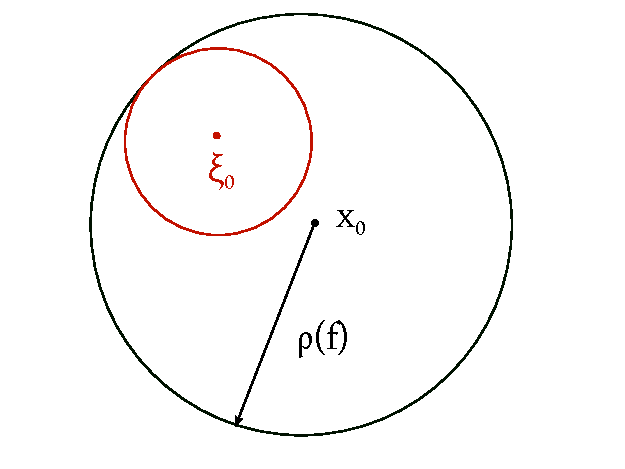
\includegraphics{img/29_expansion_on_a_different_point.pdf}
    \caption{Expansion on a different point}
    \label{img:expan}
  \end{center}
\end{figure}

Revision: Expansion on a different point ($\xi_0$ instead of $x_0$):

\[ f(z) = \sum_{k=0}^\infty a_k (z - x_0)^k = \sum_{k=0}^\infty \frac{f^{(k)}(x_0)}{k!} (z - x_0)^k \]
with $a_k = \frac{f^{(k)}(x_0)}{k!}$. $f(z) = \sum_{k=0}^\infty \tilde a_k(z - \xi_0)^k$ with $\tilde a_k = \frac{f^{(k)}(\xi_0)}{k!}$.
Compare with Figure~\ref{img:expan}.

\section{Multidimensional differential calculus} % Chapter 3

Let $V,W$ be vector space over $\mathbb K$ ($\mathbb R, \mathbb C$).
\[ \underbrace{\mathcal L(V, W)}_{\operatorname{Hom}(V, W)} = \set{\varphi: V \to W: \varphi \text{ is linear}} \]
$\operatorname{Hom}(V, W)$ has vector space properties.
$\varphi, \psi \in \mathcal L(V, W), \lambda, \mu \in \mathbb K$.
Then $\lambda \varphi + \mu \psi \in \mathcal L(V, W)$.
In general, it is feasible that to define a norm on $\mathcal L(V, W)$.
Hence, $\norm{\cdot}: \mathcal L(V, W) \to [0, \infty)$ with
\begin{enumerate}
  \item $\norm{\varphi} = 0 \iff \varphi = 0$ (zero mapping)
  \item $\forall \lambda \in \mathbb K, \varphi \in \mathcal L(V, W): \norm{\lambda \varphi} = \card{\lambda} \cdot \norm{\varphi}$.
  \item $\forall \varphi, \psi \in \mathcal L(V, W): \norm{\varphi + \psi} \leq \norm{\varphi} + \norm{\psi}$.
\end{enumerate}

\subsection{Frobenius and matrix norm}

\index{Frobenius norm}
\index{Matrix norm}
\begin{example}
  Let $\mathcal L(\mathbb R^m, \mathbb R^n) \cong \mathbb R^{n \times n}$.
  (identify linear maps with its matrix representation in regards of the canonical basis)
  \[ A \in \mathbb R^{n \times m} \qquad A = (a_{ij})_{\substack{i=1,\dots,n \\ j=1,\dots,m}} \]
  \[ \norm{A}_F = \left(\sum_{i=1}^n \sum_{j=1}^m \card{a_{ij}}^2\right)^{\frac12} \qquad \text{\enquote{Forbenius norm}} \]
  It basically works by appending the next column to the previous one. Hence, this gives a column vector. We square every entries, sum it up and take its square root (a common norm procedure).
  A norm on $\mathbb R^{n \times m}$ (a matrix) is called \emph{matrix norm} ($\mathbb C^{n \times m}$).
\end{example}

\subsection{Operator norm and bounded linear operators}

\index{Operator norm}
\begin{definition} % Definition 1
  \label{opdef}
  Let $V, W$ be normed vector spaces over $\mathbb K$. A linear map $\varphi: V \to W$ is called \emph{bounded} if $\exists m \geq 0: \norm{\varphi(x)}_W < m \cdot \norm{x}_V$ (we call this the \emph{boundedness criterion})
  such that $\norm{\varphi(x)}_W \leq m \cdot \norm{x}_V$ for all $x \in V$. % TODO The [almost] same criterion occurs twice in this sentence.

  The set $\mathcal L_b(V, W) = \set{\varphi: V \to W: \varphi \text{ is linear and bounded}}$ is a subvectorspace of $\mathcal L(V, W)$. We let
  \[ \norm{\varphi} = \inf\set{m \geq 0: \norm{\varphi(x)}_W \leq m \cdot \norm{x}_V \forall x \in V} \]
  and call $\norm{\varphi}$ the \emph{operator norm} on $\varphi$ in regards of $\norm{\cdot}_V$ and $\norm{\cdot}_W$.
\end{definition}

Regarding the subvector space property:

Let $\varphi, \psi \in \mathcal L_b(V, W), \lambda, \mu \in \mathbb K$.
Show that $\lambda \varphi + \mu \psi \in \mathcal L_b(V, W)$.

\begin{align*}
  \norm{(\lambda \varphi + \mu \psi)(x)}_W
    &= \norm{\lambda \cdot \varphi(x) + \mu \cdot \psi(x)}_W \\
    &\leq \card{\lambda} \norm{\varphi(x)}_W + \card{\mu} \norm{\varphi(x)}_W \\
    &\underbrace{\leq}_{\text{because } \varphi, \psi \text{ are bounded}} \card{\lambda} m \norm{x}_V + \card{\mu} m' \norm{x}_V \\
    &= \underbrace{\left(\card{\lambda} m + \card{\mu} m'\right)}_{= \tilde m \geq 0} \norm{x}_V
\end{align*}
hence $\lambda \varphi + \mu \psi \in \mathcal L_b(V, W)$.
$\mathcal L_b(V, W) \neq \emptyset$.

\begin{lemma} % Lemma 1
  Let $V, W$ be normed vector spaces. Then it holds for any $\varphi \in \mathcal L_b(V, W)$
  \begin{enumerate}
    \item $\norm{\varphi(x)}_W \leq \norm{\varphi} \cdot \norm{x}_V \forall x \in V$.
      Hence, $m = \norm{\varphi}$ satisfies the boundedness criterion, hence
      informally $\inf$ equals $\min$ in Definition~\ref{opdef}.
    \item
      \[ \norm{\varphi} = \sup\set{\frac{\norm{\varphi(x)}_W}{\norm{x}_V}: x \in V \setminus \set{0}} = \sup\set{\norm{\varphi(x)}_W: x \in V \text{ with } \norm{x}_V = 1} \]
    \item $\norm{\cdot}$ is a norm on $\mathcal L_b(V,W)$.
  \end{enumerate}
\end{lemma}
\begin{proof}
  \begin{enumerate}
    \item Let $m_n \geq 0$ with $m_n$ satisfies the boundedness criterion, hence
      \[ \norm{\varphi(x)}_W \leq m_n \cdot \norm{x}_V \forall x \in V \]
      and $m_n \to \norm{\varphi}$.
      The inequality retains in the limit. Thus, $\norm{\varphi(x)}_W \leq \norm{\varphi} \cdot \norm{x}_V$.
    \item Let $\tilde m = \sup\set{\frac{\norm{\varphi(x)}_W}{\norm{x}_V}: x \neq 0}$.
      Hence, $\frac{\norm{\varphi(x)}_W}{\norm{x}_V} \leq \tilde m \forall x \in V$, because $\tilde m$ is an upper bound.
      So, $\norm{\varphi(x)}_W \leq \tilde m \norm{x}_V$. Thus $\tilde m$ satisfies the boundedness criterion and $\norm{\varphi} \leq \tilde m$.

      On the opposite: Let $m$ such that the boundedness criterion is satisfied $\implies \norm{\varphi(x)}_W \leq m \cdot \norm{x}_V \forall x \in V, x \neq 0$
      and accordingly, $\frac{\norm{\varphi(x)}}{\norm{x}_V} \leq m$.
      Hence, $m$ is upper bound of $\set{\frac{\norm{\varphi(x)}}{\norm{x}_V} : X \neq 0}$, hence $m \geq \tilde m = \sup\set{\cdot}$.
      Hence, $m \geq \tilde m = \sup\set{\frac{\norm{\varphi(x)}_W}{\norm{x}_V}: x \neq 0}$.
      The statement above also holds for the infimum of $m-s$, hence $\norm{\varphi} \geq \tilde m$,
      hence $\norm{\varphi} = \tilde m = \sup\set{\frac{\norm{\varphi(x)}_W}{\norm{x}_V}: x \neq 0}$.
      Because $\set{x \in V: \norm{x} = 1} \subseteq \set{x \in V: x \neq 0}$,
      $\sup{\norm{\varphi(x)}_W: \norm{x} = 1} = \sup{\set{\frac{\norm{\varphi(x)}_W}{\norm{x}_V} : \norm{x}_V = 1}} \leq \sup\set{\frac{\norm{\varphi(x)}_W}{\norm{x}_V} : x \neq 0} = \norm{\varphi}$.

      On the opposite: Let $x \neq 0$. Then $\tilde x = \frac{x}{\norm{x}_V}$ defines a \emph{unit vector}.
      \[ \norm{\tilde x}_V = \norm{\frac{x}{\norm{x}_V}} = \frac{1}{\norm{x}_V} \cdot \norm{x}_V = 1 \]
      and
      \[ \frac{\norm{\varphi(x)}_W}{\norm{x}_V} = \frac{1}{\norm{x}_V} \norm{\varphi(x)}_W = \norm{\frac{1}{\norm{x}_V} \varphi(x)}_W \underbrace{=}_{\varphi \text{ is linear}} = \norm{\varphi(\frac{x}{\norm{x}_V})}_W = \norm{\varphi(\tilde x)} \]
      \[ \implies \forall x \neq 0: \frac{\norm{\varphi(x)}_W}{\norm{x}_V} = \norm{\varphi(\tilde x)} \leq \sup\set{\norm{\varphi(z)}_W: \norm{z}_V = 1} \]
      \[ \implies \sup\set{\frac{\norm{\varphi(x)}_W}{\norm{x}_V}: x \neq 0} \leq \sup\set{\norm{\varphi(z)}_W: \norm{z}_V = 1} \]
    \item Show that $\norm{\varphi}$ is a norm.

      \[ \norm\varphi = 0 \iff \forall x \in V: \norm{\varphi(x)}_W \leq 0 \cdot \norm{x}_W \]
      hence $\varphi(x) = 0 \forall x \in V$ and accordingly, $\varphi = 0$ in $\mathcal L(V, W)$.
      \[ \norm{\lambda \varphi} = \sup\set{\norm{\lambda \varphi(x)}_W: \norm{x}_V = 1} = \sup\set{\card{\lambda} \norm{\varphi(x)}_W: \norm{x}_V = 1} \]
      \[ = \card{\lambda} \sup\set{\norm{\varphi(x)}_W: \norm{x}_V = 1} = \card{\lambda} \norm{\varphi} \]
      Triangle inequality:
      Let $\varphi, \psi \in \mathcal L_b(V,W)$.
      \begin{align*}
        \norm{\varphi(x) + \psi(x)}_W
          &\underbrace{\leq}_{\text{triangle inequality in } W} \norm{\varphi(x)}_W + \norm{\psi(x)}_W \\
          &\leq \norm \varphi \cdot \norm{x}_V + \norm \psi \cdot \norm{x}_V = (\norm{\varphi} + \norm{\psi}) \cdot \norm{x}
      \end{align*}
      By (1.), $\norm{\varphi} + \norm{\psi}$ satisfies the boundedness criterion for the linear map $\varphi + \psi$.
      Hence, $\norm{\varphi + \psi} \leq \norm{\varphi} + \norm{\psi}$.
  \end{enumerate}
\end{proof}

\begin{remark}
  \begin{itemize}
    \item $\norm{A}_F$ is no operator norm on $\mathcal L(\mathbb R^m, \mathbb R^n)$.
    \item Boundedness of linear mappings is required to define $\norm{\varphi}$.
  \end{itemize}
  We consider special case $V = \mathbb R^m, W = \mathbb R^n$.
  \[ \norm{\cdot}_V = \norm{\cdot}_\infty \qquad \norm{\cdot}_W = \norm{\cdot}_\infty \]
  Let $A \in \mathbb R^{n\times m}$ ($\mathcal L(\mathbb R^m, \mathbb R^n)$).
  Then
  \begin{align*}
    \norm{Ax}_\infty
      &= \max\set{\card{(Ax)_i}: i = 1, \dots, n} \\
      &= \max\set{\card{\sum_{j=1}^m a_{ij} x_j}: i = 1, \dots, n} \\
      &\leq \max\set{\sum_{j=1}^m \card{a_{ij}} \cdot \underbrace{\card{x_j}}_{\leq \norm{x}_{\infty}}: i = 1, \dots, n} \\
      &\leq \max\set{\norm{x}_\infty \cdot \sum_{j=1}^m \card{a_{ij}}: i = 1, \dots, n} \\
      &= \underbrace{\max\set{\sum_{j=1}^m \card{a_{ij}}: i = 1, \dots, n}}_{= m} \cdot \norm{x}_\infty \\
      &= m \cdot \norm{x}_\infty
  \end{align*}
  Hence the boundedness criterion is satisfied.
  $A$ is bounded in regards of $\norm{\cdot}_\infty$ in the preimage and image space.
  By the norm equivalence theorem, it follows that $A$ is bounded in regards of arbitrary norms on $\mathbb R^m$, and accordingly $\mathbb R^n$.
\end{remark}

\dateref{2018/05/17}

Further remarks:
\begin{remark}
  A linear map $A: \mathbb R^m \to \mathbb R$ is always bounded. Thus,
  \[ \norm{Ax_1 - Ax_2}_{\mathbb R^n} = \norm{A(x_1 - x_2)}_{\mathbb R^n} \leq \norm{A} \norm{x_1 - x_2}_{\mathbb R^m} \]
  So every linear map $A: \mathbb R^m \to \mathbb R^n$ is Lipschitz \emph{continuous} with Lipschitz constant $\norm{A}$.
\end{remark}

The considerations above hold for arbitrary finite-dimensional normed vector spaces $V$ and $W$ (over $\mathbb K = \mathbb R, \mathbb C$).

\begin{lemma} % Lemma 2
  Let $X, Y$ and $Z$ be normed vector spaces.
  Let $A: X \to Y$ be linear and bounded. Let $B: Y \to Z$ be linear and bounded.
  Then
  \[ B \cdot A: X \to Z \]
  is also bounded and
  \[ \norm{B \cdot A} \leq \norm{B} \cdot \norm{A} \]
\end{lemma}

\begin{proof}
  Let $x \in X$ be arbitrary and $BAx = B(Ax) \in Z$ and
  \[ \norm{BAx}_Z = \norm{B(Ax)}_Z \overbrace{\leq}_{B \text{ is bounded}} \norm{B} \norm{Ax}_Y \underbrace{\leq}_{A \text{ is bounded}} \norm{B} \cdot \norm{A} \norm{x}_X \]
  Hence $m = \norm B \norm A$ satisfies the boundedness criterion for the linear map $B \cdot A: X \to Z$. Because $\norm{B\cdot A}$ is the smallest constant
  for which the boundedness criterion holds, it follows that $\norm{BA} \leq \norm B \norm A$.
\end{proof}

\subsection{Landau notation}
% TODO on the date 2018/05/17, I might have mixed up big-o and small-o notation. Review required
\begin{definition}[Landau $\mathbb O$ symbols] % Definition 2
  Let $h, g: D \subseteq \mathbb R^n \to \mathbb R$ and $D$ is open, $a \in D$.
  \begin{enumerate}
    \item We denote $h = \mathcal O(g)$ in $a$ (German pronunciation: \foreignlanguage{german}{h ist groß $\mathcal O$ von $g$}) iff
      $\exists U \subseteq D$ neighborhood of $a$ in $D$ and $\exists r: U \to \mathbb R$ with $r$ bounded such that $h(x) = r(x) \cdot g(x) \forall x \in U$.
      Thus,
      \[ \card{\frac{h(x)}{g(x)}} = \card{r(x)} \leq M \qquad \forall x \in U \]
      ($g(x) = 0$ iff $h(x) = 0$)
    \item We denote $h = o(g)$ in $a$ (German pronunciation: \foreignlanguage{german}{h ist klein $o$ von $g$}) iff $\exists U \subseteq D$, with $U$ being the neighborhood of $a$, and $r: U \to \mathbb R$ such that $\lim_{x\to a} r(x) = 0$
    and $h(x) = r(x) \cdot g(x) \forall x \in U$. In that sense,
      \[ \lim_{x \to a} \frac{h(x)}{g(x)} = 0 \]
      Most often, $\mathcal O(\underbrace{\norm{x - x_0}^n}_{g(x)})$ will be used (in this context of differentiability here) with $a = x_0$.
  \end{enumerate}
\end{definition}

\subsection{Multidimensional derivative of a function}
\begin{definition}[Definition of the derivative of a function]
  \[ f: D \subseteq \mathbb R^m \to \mathbb R^n \qquad D \text{ is open}, x_0 \in D \]
  \[ f(x) = \begin{bmatrix} f_1(x) \\ f_2(x) \\ \vdots \\ f_n(x) \end{bmatrix} \in \mathbb R^n \]
  \[ f_i(x) = f_i\left(\begin{bmatrix} x_1 \\ x_2 \\ \vdots \\ x_m \end{bmatrix}\right) = f_i(x_1, x_2, \dots, x_m) \in \mathbb R \]
\end{definition}

\begin{remark}
  First trial to define the derivative:
  \[ f'(x_0) \coloneqq \lim_{x\to x_0} \frac{\overbrace{f(x) - f(x_0)}^{\in \mathbb R^n}}{\underbrace{x - x_0}_{\in \mathbb R^m}} \]
  Does not work because of incompatibility of dimensions (and we cannot divide vectors).
\end{remark}

\begin{remark}
  We use Taylor's Theorem to characterize $f'(x_0)$. A Taylor polynomial of 1st degree is given by
  \[ f(x) = f(x_0) + f'(x_0) (x - x_0) + R_f^2(x; x_0) \]
  and $R_f^2(x; x_0) = r(x) (x - x_0)$ with $\lim_{x\to x_0} r(x) = 0$.
  Hence,
  \[ f(x) - f(x_0) - f'(x_0)(x - x_0) = \mathcal O(x - x_0) \]
  or we insert the absolute operators:
  \[ \card{f(x) - f(x_0) - f'(x_0) (x - x_0)} = \card{r(x)} \cdot \card{x - x_0} = o(\card{x - x_0}) \]
  where $(f(x) - f(x_0)) \in \mathbb R^n$ for the multidimensional case
  and $(x - x_0) \in \mathbb R^m$ for the multidimensional case. Thus,
  \[ = \mathcal O(\card{x - x_0}) \]
\end{remark}

\begin{definition} % Definition 3
  \label{defp}
  Let $f: D \subseteq \mathbb R^m \to \mathbb R^n$, $D$ is open and $x_0 \in D$.
  We say, \enquote{f is differentiable in $x_0$} (specifically, \enquote{Frech\'et differentiable})
  if there exists $A \in \mathbb R^{n \times m}$ such that
  \[ \norm{f(x) - f(x_0) - A(x - x_0)}_{\mathbb R^n} = o(\norm{x - x_0}_{\mathbb R^m}) \]
  We call this condition \emph{differentiability condition}.
  $A$ is a linear approximation of $f$ in $x_0$.
  Because of norm equivalence on $\mathbb R^n$, and accordingly $\mathbb R^m$,
  it is irrelevant which norm $\norm{\cdot}_{\mathbb R^n}$ and $\norm{\cdot}_{\mathbb R^m}$ is chosen.
\end{definition}

\begin{lemma} % Lemma 3
  Let $f$ be, as in Definition~\ref{defp}, differentiable in $x_0$.
  Then the linear approximation $A$, by the differentiability condition, is uniquely determined.
\end{lemma}

\begin{proof}
  Assume $A, B \in \mathbb R^{n\times m}$ satisfy the differentiability condition.
  Let $r > 0$ such that $K_r(x_0) \subseteq D$ (feasible because $D$ is open and $x_0 \in D$).
  Furthermore let $v \in \mathbb R^m$ and $\norm{v} < r$, hence $x = x_0 + v \in K_r(x_0) \subset D$
  and $v = x - x_0$.
  \[ \norm{(A - B) v} = \norm{Av - Bv} = \norm{A(x - x_0) - B(x - x_0)} \]
  \[ = \norm{f(x) - f(x_0) - B(x - x_0) - (f(x) - f(x_0) - A(x_0 - x_0))} \]
  \[ \leq \norm{f(x) - f(x_0) - B(x - x_0)} + \norm{f(x) - f(x_0) - A(x - x_0)} \]
  by the differentiability criterion
  \[ r(x) \cdot \norm{x - x_0} + \tilde r(x) \norm{x - x_0} \]
  with $\lim_{x\to x_0} r(x) = \lim_{x\to x_0} \tilde r(x) = 0$. Hence, for $\hat r(x) = r(x) + \tilde r(x)$,
  \[ \norm{(A - B) v} \leq \hat r(x) \norm{x - x_0} = \hat r(x) \norm{v} = \mathcal O(\norm{v}) \text{ in } x_0 \]
  (Thus $\lim_{x\to x_0} \hat r(x) = 0$)

  Show: $(A - B)w = 0 \forall w \in \mathbb R^m$. Assume $\exists w \in \mathbb R^m, w \neq 0$ with $(A - B)w \neq \diameter$.
  For $\card{\alpha} < \frac r{\norm{w}}$ (with $r$ as radius of the sphere),
  \[ \norm{\alpha w} = \card{\alpha} \norm{w} < \frac{r}{\norm{w}} \cdot \norm{w} = r \]
  Let $v = \alpha w$. Then
  \[ \norm{(A - B) v} = \card{\alpha} \norm{(A - B) w} \leq \hat r(x) \norm{\alpha w} = \card{\alpha} \hat r(x) \cdot \norm{w} \]
  \[ \implies \norm{(A - B) w} \leq \underbrace{\hat r(x)}_{\xrightarrow{\text{for } x \to x_0} 0} \cdot \underbrace{\norm w}_{\text{constant}} \]
  \[ \implies (A - B) w = 0 \]
  This contradicts with our assumption.

  Therefore, $Aw = Bw \forall w \in \mathbb R^m$, hence $A = B$.
\end{proof}

\subsection{Frech\'et derivative}
\index{Frech\'et derivative}
\begin{definition}[Part 2 of Definition~\ref{defp}] % Definition 3
  If $f$ is differentiable in $x_0$, then we call the uniquely determined linear map $A$ the \enquote{Frech\'et derivative} of $f$ in $x_0$
  and denote $A = Df(x_0)$. An alternative notations are $f'(x_0)$ and $D_{x_0}f$.
\end{definition}

\begin{lemma} % Lemma 4
  Let $f: D \to \mathbb R^n$, $D \subseteq \mathbb R^m$ open, $x_0 \in D$.
  If $f$ is differentiable in $x_0$, then $f$ is also continuous in $x_0$.
\end{lemma}

\begin{proof}
  Let $x \in D$. Then,
  \begin{align*}
    \norm{f(x) - f(x_0)}_{\mathbb R^n}
      &= \norm{f(x) - f(x_0) - Df(x_0) \cdot (x - x_0) + Df(x_0) (x - x_0)} \\
      &\leq \norm{f(x) - f(x_0) - Df(x_0) (x - x_0)} + \norm{Df(x_0) (x - x_0)} \\
      &\leq r(x) \cdot \underbrace{\norm{x - x_0}}_{\to 0 \text{ for } x \to x_0} + \overbrace{\norm{\underbrace{Df(x_0)}_{\in \mathbb R^{n\times m}}}}^{\text{constant}} \cdot \underbrace{\norm{x - x_0}}_{\to 0 \text{ for } x \to x_0} \\
      &\to 0 \text{ for } x \to x_0
  \end{align*}
  Hence $f$ is continuous in $x_0$.
\end{proof}

\begin{lemma} % Lemma 5
  \label{lem5}
  Let $f,g: D \subseteq \mathbb R^m \to \mathbb R^n$. Let $f$ and $g$ be differentiable in $x_0 \in D$.
  Let $\lambda \in \mathbb R$. Then,
  \begin{enumerate}
    \item $f + g$ is differentiable in $x_0$ with
      \[ D(f + g)(x_0) = Df(x_0) + Dg(x_0) \]
    \item $\lambda f$ is differentiable in $x_0$ and
      \[ D(\lambda f)(x_0) = \lambda Df(x_0) \]
  \end{enumerate}
  Thus differentiability is a linear operation on the vector space's appropriate differentiable functions.
\end{lemma}

\begin{proof}
  Let $F \coloneqq \norm{(f + g)(x) - (f + g)(x_0) - [Df(x_0) + Dg(x_0)](x - x_0)]}$
  with $[Df(x_0) + Dg(x_0)] = D(f + g)(x_0)$.
  Show that $F = o(\norm{x - x_0})$.
  \begin{align*}
    F &\leq \norm{f(x) - f(x_0) - Df(x_0)(x - x_0)} + \norm{g(x) - g(x_0) - Dg(x_0)(x - x_0)} \\
      &= o(\norm{x - x_0}) + o(\norm{x - x_0}) \\
      &= o(\norm{x - x_0})
  \end{align*}
  For $\lambda f$ it holds analogously.
\end{proof}

\begin{lemma} % Lemma 6
  Let $C: D \to \mathbb R^n$. $C(x) = k \in \mathbb R^n$ is constant.
  Then $C$ is differentiable in every point $x_0 \in D$ and $D C(x_0) = 0 \in \mathbb R^{n\times m}$.
  Let $A: \mathbb R^m \to \mathbb R^n$ be linear. Then $A$ is differentiable in every point $x_0 \in \mathbb R^m$ and $DA(x_0) = A$.

  Let $f(x) = k + Ax: \mathbb R^m \to \mathbb R^n$ be linear affine, then $f$ is differentiable in every point $x_0 \in \mathbb R^m$ with $Df(x_0) = A$.
\end{lemma}

\begin{proof}
  \[ \norm{c(x) - c(x_0) - 0 \cdot (x - x_0)} \]
  where $0$ denotes the zero-matrix.
  \[ = \norm{k - k} = \norm{0} = 0 = o(\norm{x - x_0}) \]
  Hence $0$ satisfies the differentiability condition for $c$.
  \[ \implies 0 = Dc(x_0) \]
  in the linear case
  \[ \norm{Ax - Ax_0 - A(x - x_0)} = \norm{Ax - Ax_0 - Ax + Ax_0} = 0 = o({x - x_0}) \]
  hence $DA(x_0) = A$.
  Affine: use Lemma~\ref{lem5}.
  \[ D(k + A)(x_0) = \underbrace{Dk(x_0)}_{=0} + \underbrace{DA(x_0)}_{= A} = A \]
  This is analogous to the one-dimensional case:
  \[ (k + ax)' = a \]
\end{proof}

\subsection{Chain rule}
\begin{theorem}[Chain rule in multiple dimensions]
  Let $D \subseteq \mathbb R^l$ be open. Let $E \subseteq \mathbb R^m$ be open.
  Let $f: D \to \mathbb R^m$ such that $f(D) \subseteq E$ and $g: E \to \mathbb R^n$.
  Compare with Figure~\ref{chainrule}.

  \begin{figure}[t]
    \begin{center}
      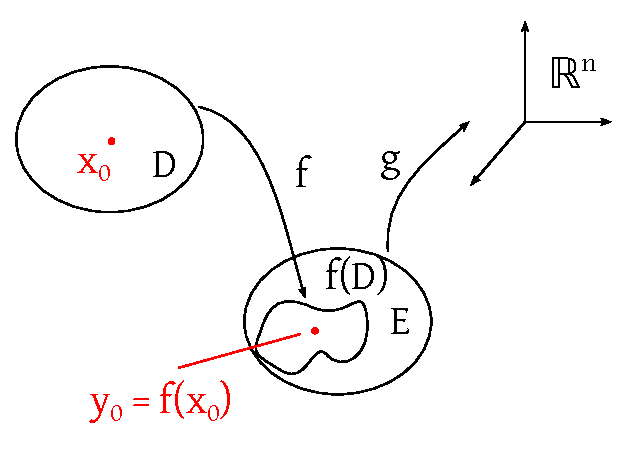
\includegraphics{img/30_fg.pdf}
      \caption{Chain rule in multiple dimensions}
      \label{chainrule}
    \end{center}
  \end{figure}

  Let $f$ in $x_0$ be differentiable and $g$ in $y_0 = f(x_0)$ is differentiable.
  Then also $g \circ f: D \to \mathbb R^n$ is differentiable in $x_0$ and
  \[ \underbrace{D(g \circ f)(x_0)}_{\in \mathbb R^{n \times l}} = \underbrace{Dg(f(x_0))}_{\in \mathbb R^{n \times m}} \underbrace{Df(x_0)}_{\in \mathbb R^{m \times l}} \]
  (The dimensions match.)
\end{theorem}
\begin{proof}
  $(g \circ f)(x)$ is differentiable in $x_0$ iff
  \[ \lim_{x \to x_0} \frac{\norm{g(f(x_0)) - g(f(x_0)) - D g(f(x_0)) \cdot Df(x_0) \cdot (x - x_0)}}{\norm{x - x_0}} = 0 \]
  according to Frech\'et differentiability. This is equivalent to 
  \[ \frac{\norm{g(f(x_0)) - g(f(x_0)) - D g(f(x_0)) \cdot Df(x_0) \cdot (x - x_0)}}{\norm{x - x_0}} < \varepsilon \]
  for any bounded $\varepsilon$.
  Let $0 < \varepsilon < 2$.
  Show that
  \[ \frac1{\norm{x - x_0}} \norm{g(f(x)) - g(f(x_0)) - Dg(y_0) \cdot Df(x_0) (x - x_0)} < \varepsilon \]
  for sufficiently small $\norm{x - x_0}$ with $x \neq x_0$.
  \begin{align*}
    &\frac1{\norm{x - x_0}} \norm{g(f(x)) - g(f(x_0)) - Dg(y_0) \cdot Df(x_0) (x - x_0)} \\
    &= \frac1{\norm{x - x_0}} \| g(f(x)) - g(f(x_0)) {\color{blue} -} Dg(f(x_0)) \cdot (f(x) - f(x_0)) \\
    &{\color{blue} +} Dg(f(x_0)) (f(x) - f(x_0)) - Dg(f(x_0)) Df(x_0) (x - x_0) \| \\
  \intertext{recognize that we have a common factor $Dg(f(x_0))$}
    &\leq \frac{1}{\norm{x - x_0}} \norm{g(f(x)) - g(f(x_0)) - Dg(f(x_0))(f(x) - f(x_0))} \\
    &+ \frac{1}{\norm{x - x_0}} \norm{Dg(y_0)} \norm{f(x) - f(x_0) - Df(x_0)(x - x_0)} \\
    &\eqqcolon (I) + (II)
  \end{align*}
  Choose $\delta_1 > 0$ such that $\norm{x - x_0} < \delta_1 \implies$
  \[ \frac{1}{\norm{x - x_0}} \cdot \norm{f(x) - f(x_0) - Df(x_0) (x - x_0)} < \frac{\varepsilon}2 \frac{1}{\norm{Dg(y_0)} + 1} \]
  is feasible, because $f$ is differentiable in $x_0$.
  \[ \frac{\varepsilon}{2} \cdot \frac{1}{\norm{Dg(y_0)} + 1} < \frac22 = 1 \]
  so it also holds that
  \[ \norm{f(x) - f(x_0) - Df(x_0) (x - x_0)} < 1 \cdot \norm{x - x_0} \]
  By the reverse triangle inequality,
  \[ \norm{f(x) - f(x_0) - Df(x_0) (x - x_0)} \geq \norm{f(x) - f(x_0)} - \norm{Df(x_0) (x - x_0)} \]
  \[ \geq \norm{f(x) - f(x_0)} - \norm{Df(x_0)} \cdot \norm{x - x_0} \]
  \[ \implies \frac{\norm{f(x) - f(x_0)}}{\norm{x - x_0}} \leq \norm{Df(x_0)} + 1 \]

  \dateref{2018/05/24}

  \[ \norm{f(x) - f(x_0)} - \norm{Df(x_0)} \norm{x - x_0} < 1 \norm{x - x_0} \]
  hence, for $x \neq x_0$
  \[ \frac{\norm{f(x) - f(x_0)}}{\norm{x - x_0}} < \norm{Df(x_0)} + 1 \]

  $g$ is differentiable in $y_0 = f(x_0)$. Hence, we can choose $\delta_g > 0$ such that $\forall y \in E$ with $\norm{y - y_0} < \delta_g$
  it holds that
  \[ \norm{g(y) - g(y_0) - Dg(y_0) \cdot (y - y_0)} < \frac{\varepsilon}{2 \left(\norm{Df(x_0) + 1}\right)} \norm{y - y_0} \]
  Because $f$ is continuous in $x_0$, there exists $\delta_2 > 0$ such that $x \in D$ and $\norm{x - x_0} < \delta_2 \implies \norm{f(x) - f(x_0)} < \delta_g$.
  Now let $\delta = \min(\delta_1, \delta_2) > 0$. Then
  \[ I \coloneqq \frac{1}{\norm{x - x_0}} \norm{g(f(x)) - g(f(x_0)) - Dg(f(x_0)) \cdot (f(x) - f(x_0))} \]
  Let $y = f(x), y_0 = f(x_0)$.
  Because $\norm{f(x) - f(x_0)} < \delta_g$ gives $\norm{x - x_0} < \delta_2$
  \[ \implies I < \frac{\varepsilon}{2 \left(\norm{Df(x_0)} + 1\right)} \underbrace{\frac{\norm{f(x) - f(x_0)}}{\norm{x - x_0}}}_{< \norm{Df(x_0)} + 1} < \frac\varepsilon2 \]
  \[ II \coloneqq \norm{Dg(y_0)} \frac{1}{\norm{x - x_0}} \norm{f(x) - f(x_0) - Df(x_0) (x - x_0)} \]
  \[ < \norm{Dg(y_0)} \cdot \frac{\varepsilon}{2} \cdot \frac{1}{\norm{Dg(y_0)} + 1} < \frac\varepsilon2 \]
  hence, $I + II < \varepsilon$ for $\norm{x - x_0} < \delta$.
\end{proof}

\subsection{Differentiability on $D$}
\index{Differentiable on $D$}
\begin{definition}
  Let $f: D \subseteq \mathbb R^m \to \mathbb R^n$ be differentiable in every point $x \in D$.
  Then we are used to say \enquote{$f$ is differentiable \emph{on} $D$}.

  In this case, we call the map
  \[ x \mapsto Df(x) \]
  \[ D \subseteq \mathbb R^m \to \mathbb R^{n \times m} \]
  the mapping function of $f$ (dt. \foreignlanguage{german}{Abbildungsfunktion}).
  If this function is continuous (in terms of $\norm{\cdot}_{\mathbb R}$ or $\norm{\cdot}_{\mathbb R^{n \times m}}$ \dots operator norm),
  then $f$ is called continuously differentiable on $D$.
\end{definition}

\begin{remark}
  To define the differentiability of $f$, we require $x_0$ to be an accumulation point of $D$.
  So $x_0$ might also be a point on the boundary of $D$.
\end{remark}

\subsubsection{Determination of $Df(x_0) \in \mathbb R^{n \times m}$}

\begin{definition}
  \label{defin5}
  Let $f: D \subseteq \mathbb R^m \to \mathbb R^n$ be given.
  $D$ is open, $x_0 \in D$, $v \in \mathbb R^m$ is arbitrary, but $v \neq 0$.
  We consider $t \mapsto f(x_0 + tv)$ defined on $(-\frac{r}{\norm{v}}, \frac{r}{\norm{v}})$
  for $r > 0$ such that $K_r(x_0) \subseteq D$.
  \[ \left(-\frac{r}{\norm{v}}, \frac{r}{\norm{v}}\right) \subseteq \mathbb R \to \mathbb R^n \]
  Compare with Figure~\ref{img:set5}.

  \index{Directional derivative}
  We define $df(x_0; v) = \lim_{t \to 0} \frac1{t} (f(x_0 + tv) - f(x_0))$ if this limit exists. $df(x_0, v)$ is called \emph{directional derivative} of $f$ in $x_0$ in direction $v$. It is also called \emph{Gateaux derivative of $f$ in $x_0$ in direction $v$}.
\end{definition}

\begin{figure}[t]
  \begin{center}
    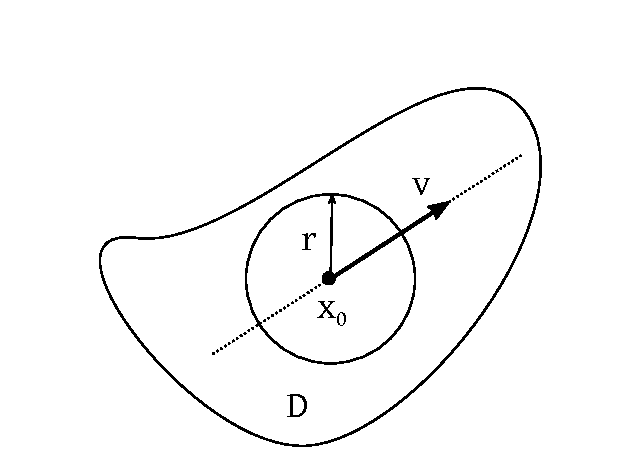
\includegraphics{img/31_setting.pdf}
    \caption{Setting in Definition~\ref{defin5}. The line is given by $g = \set{x_0 + tv: t \in \mathbb R}$}
    \label{img:set5}
  \end{center}
\end{figure}

\begin{remark}
  How does it go together?
  
  Derivative $Df(x_0)$ and $df(x_0; \cdot)$.
  Assumption: Let $f$ be differentiable in $x_0$.
  We define $l_{x_0,v}(t) = x_0 + tv$
  where $tv$ is the linear part.
  \[ l_{x_0,v}: \left(-\frac{r}{\norm{v}}, \frac{r}{\norm{v}}\right) \to D \]
  $l_{x_0,v}$ is linear affine from $\mathbb R$ to $\mathbb R^m$.
  \[ Dl_{x_0,v}(0) = V \in \mathbb R^{m \times 1} \]
  with $V$ as linear part of $l_{x_0,v}$.
  \[ l_{x_0, v}(0) = x_0 \]
  \[ f(x_0 + tv) = f \circ l_{x_0,v}(t) \]
  Therefore ($\to$ chain rule)
  \[ D(f \circ l_{x_0,v})(0) = Df(l_{x_0,v}(0)) \cdot Dl_{x_0,v}(0) = Df(x_0) \cdot v \]
  On the other side,
  \[ 0 = \underbrace{\lim_{t\to 0} \frac{1}{\card{t}} \card{f_{x_0,v}(t) - f_{x_0,v}(0) - Df_{x_0,v}(0) \cdot t}}_{=0} \]
  \[ = \lim_{t\to0} \frac{1}{\card{t}} \card{f(x_0 + tv) - f(x_0) - Df_{x_0,v}(0) \cdot t} \]
  \[ = \lim_{t\to0} \card{\frac{f(x_0 + tv) - f(x_0)}{t} - Df_{x_0,v}(0)} = 0 \]
  therefore
  \[ Df_{x_0,v}(0) = \lim_{t\to 0} \frac{f(x_0 + tv) - f(x_0)}{t} = df(x_0;v) \]
\end{remark}

\begin{lemma} % Lemma 7
  Let $f: D \subseteq \mathbb R^m \to \mathbb R^n$ in $x_0 \in D$ (Frech\'et) differentiable with derivative $Df(x_0)$.
  Then also the directional derivative $df(x_0; v)$ for every direction $v \in \mathbb R^m \setminus \set{0}$ and % TODO: ... exists?
  \[ df(x_0; v) = Df(x_0) \cdot v \]
\end{lemma}

\begin{remark}
  $v \mapsto df(x_0; v)$ is linear. We can derive the structure of the derivative matrix.
  Let $f$ as above. Let $\mathcal B = \set{e_1, \dots, e_m}$ be the canonical basis in $\mathbb R^m$.
  Then: $Df(x_0) \cdot e_j$ is the $j$-th column of $Df(x_0)$ for $j=1,\dots,m$.
  On the other hand,
  \[ Df(x_0) \cdot e_j = df(x_0; e_j) = \lim_{t\to0} \frac1{t} \left[f(x_0 + te_j) - f(x_0)\right] \]
  \[
    = \begin{bmatrix}
      \lim_{t\to 0} \frac1t \left(f_1(x_0 + te_j) - f_1(x_0)\right) \\
      \vdots \\
      \lim_{t\to 0} \frac1t \left(f_n(x_0 + te_j) - f_n(x_0)\right) \\
    \end{bmatrix}
    \text{ for }
    f(x) = \begin{bmatrix} f_1(x) \\ \vdots \\ f_n(x) \end{bmatrix} \in \mathbb R^n
  \]
\end{remark}
\begin{remark}[Notation]
  Consider $x$ instead of $x_0$
  \[ x = \begin{bmatrix} x_1 \\ \vdots \\ x_m \end{bmatrix} = [x_1, \dots, x_m]^t \]
  Instead of $f(x) = f\left(\begin{bmatrix} x_1 \\ x_2 \\ \vdots \\ x_m \end{bmatrix}\right)$
  we also write $f(x_1, x_2, \dots, x_m)$.
\end{remark}

\subsection{Partial derivative and Jacobi matrix}
\index{Partial derivative}
\begin{definition} % Definition 6
  Let $f: D \to \mathbb R^n$, $x \in D$ as above. $f$ is differentiable in $x$. Then we let
  \begin{align*}
    \frac{\partial f}{\partial x_j}(x)
      &= df(x; e_j) = \lim_{t\to0} \frac1t \left[f(x + te_j) - f(x)\right] \\
      &= \lim_{t\to0} \frac1t \left[f(x_1, \dots, x_j + t, \dots, x_m) - f(x_1, \dots, x_j, \dots, x_m)\right]
  \end{align*}
  and we call $\frac{\partial f}{\partial x_j} (x)$ the \emph{partial derivative} of $f$ of variable $x_j$ in point $x$.
  
  Notations for $\frac{\partial f}{\partial x_j}$:
  \[ f_{x_j} \qquad f_j \qquad \partial_j f \]
  The second notation is ambiguous. We will prefer the last one.
\end{definition}

\index{Jacobi matrix}
\begin{remark}
  \[
    \frac{\partial f}{\partial x_j}(x_0) =
    \begin{bmatrix}
      df_1(x; e_j) \\
      df_2(x; e_j) \\
      \vdots \\
      df_n(x; e_j) \\
    \end{bmatrix}
    = \begin{bmatrix}
      \frac{\partial f_1}{\partial x_j}(x) \\
      \vdots \\
      \frac{\partial f_n}{\partial x_j}(x)
    \end{bmatrix}
    \in \mathbb R^n
  \]
  Because $\frac{\partial f}{\partial x_j}(x)$ is the $j$-th column of $Df(x_0)$,
  we get
  \[ \left(Df(x)\right)_{i,j} = \frac{\partial f_i}{\partial x_j}(x) = \partial_j f_i(x) \]
  We say, $Df(x) = (\partial_j f_i(x))_{\substack{i = 1,\dots,n \\ j = 1,\dots,m}}$ is the \emph{Jacobi matrix} of $f$.
\end{remark}

\begin{remark}
  The Jacobi matrix can exist even though the derivative does not exist.
  If the derivative exists, the Jacobi matrix exists for sure.
\end{remark}

\begin{remark}
  \[ \frac{\partial f}{\partial x_j} = \lim_{t\to0} \frac1t \left[f(x_1, \dots, x_j+t, \dots, x_m) - f(x_1, \dots, x_j, \dots, x_n)\right] \]
  Thus, consider $x_j$ as derivation variable and all $x_k$ for $k \neq j$ as constant parameters.
\end{remark}

\begin{example}
  Consider $f: \mathbb R^3 \to \mathbb R^2$ with
  \[
    f(x_1, x_2, x_3) = \begin{bmatrix}
      x_1 x_3^2 + \sin(x_1 x_3) \\
      \frac{x_2^2}{x_1^2 + 1}
    \end{bmatrix}
  \]
  \[
    \partial_1 f(x_1, x_2, x_3) = \begin{bmatrix}
      1 \cdot x_3^2 \\
      -x_2^2 (x_1^2 + 1)^{-2} \cdot 2x_1
    \end{bmatrix} = \begin{bmatrix}
      x_3^2 \\
      -2 \frac{x_1 x_2^2}{(x_1^2 + 1)^2}
    \end{bmatrix}
  \] \[
    \partial_2 f(x_1, x_2, x_3) = \begin{bmatrix}
      x_3 \cos(x_2 x_3) \\
      \frac{2x_2}{x_1^2 + 1}
    \end{bmatrix}
  \] \[
    \partial_3 f(x_1, x_2, x_3) = \begin{bmatrix}
      2x_1 x_3 + x_2 \cos(x_2 x_3) \\
      0
    \end{bmatrix}
  \]
  Jacobi-Matrix
  \[
    Df(x)
    = \left[\frac{\partial f_i}{\partial x_j}\right]_{\substack{i = 1,\dots,2 \\ j = 1,\dots,3}}
    = \begin{bmatrix}
      x_3^2 & x_3 \cos(x_2 x_3) & 2 x_1 x_3 + x_2 \cos(x_2 x_3) \\
      - \frac{2x_1 x_2^2}{(x_1^2 + 1)^2} & \frac{2x_2}{x_1^2 + 1} & 0
    \end{bmatrix}
  \]
\end{example}

\begin{remark}
  Existence of partial derivatives of $f$ does not suffice to ensure Frech\'et-differentiability.
\end{remark}

\dateref{2018/05/29}

Usually, we always have to point out which norm is used to define differentiability.
Of course, in $\mathbb R$ itself, all norms are equivalent.

\begin{remark}
  Let $f: D \subseteq \mathbb R^m \to \mathbb R^n$ be given.
  Let $\norm{\cdot}_{1,m}$ and $\norm{\cdot}_{2,m}$ be two equivalent norms on $\mathbb R^m$ (norm equivalence theorem)
  and $\norm{\cdot}_{1,n}$ and $\norm{\cdot}_{2,n}$ are equivalent norms on $\mathbb R^n$.

  Let $f$ in $x_0 \in D$ be differentiable in regards of $\norm{\cdot}_{1,m}$ and $\norm{\cdot}_{1,n}$.
  Then also $f$ is differentiable in $x_0$ in regards of $\norm{\cdot}_{2,m}$ and $\norm{\cdot}_{2,n}$.

  \emph{Rationale:} Let $c \norm{x}_{2,m} \leq \norm{x}_{1,m} \leq C \norm{x}_{2,m}$ and
  $k \norm{y}_{2,n} \leq \norm{y}_{1,n} \leq K \norm{y}_{2,n}$, then
  \[ \frac{\norm{f(x) - f(x_0) - A(x - x_0)}_{2,n}}{\norm{x - x_0}_{2,m}} \]
  \[ \leq \frac{\frac1k \norm{f(x) - f(x_0) - A(x - x_0)}_{1,n}}{\frac1c \norm{x - x_0}_{1,m}} \]
  \[ = \frac ck \underbrace{\frac{\norm{f(x) - f(x_0) - A (x - x_0)}_{1,n}}{\norm{x - x_0}_{1,m}}}_{\xrightarrow{x \to x_0} 0} \]

  Let $f: D \subseteq \mathbb R^m \to \mathbb R^n$, $f(x) = \begin{bmatrix} f_1(x) \\ \vdots \\ f_n(x) \end{bmatrix}$.
  Then $f$ is differentiable in $x_0 \in D \iff f_k: D \to \mathbb R$ is differentiable for all $k \in \set{1, \dots, n}$.
  
  \emph{Rationale:} Let $f$ be differentiable in $x_0$. Let $A = \begin{bmatrix} a_1 \\ \vdots \\ a_n \end{bmatrix}$ be the derivative of $f$.
  Let $a_k$ be the rows of $A$. $f$ is differentiable in $x_0$, so
  \[ \frac{\norm{f(x) - f(x_0) - A(x - x_0)}_{\infty}}{\norm{x - x_0}} \xrightarrow{x \to x_0} 0 \]
  \[ \iff \frac{\card{f_n(x) - f_k(x) - a_k(x - x_0)}}{\norm{x - x_0}} \xrightarrow{x \to x_0} 0 \]
  where $a_k$ is a row vector and $x-x_0$ is a column vector and $k \in \set{1, \dots, n}$.
  \[ \iff f_k \text{ is differentiable in } x_0 \]
\end{remark}

\begin{example}[Counterexample]
  We define $f: \mathbb R^2 \to \mathbb R$.
  \[
    f(x_1, x_2) = \begin{cases}
      \frac{x_1^2 x_2}{x_1^2 + x_2^2} & \text{ for } \begin{bmatrix} x_1 \\ x_2 \end{bmatrix} \neq \begin{bmatrix} 0 \\ 0 \end{bmatrix} \\
      0 & \text{ for } \begin{bmatrix} x_1 \\ x_2 \end{bmatrix} = \begin{bmatrix} 0 \\ 0 \end{bmatrix} \\
    \end{cases}
  \]
  Partial derivatives exist in every point $\begin{bmatrix} x_1 \\ x_2 \end{bmatrix} \neq \begin{bmatrix} 0 \\ 0 \end{bmatrix}$.
  \[ \partial_1 f(x_1, x_2) = \frac{2 x_1 x_2 (x_1^2 + x_2^2) - x_1^2 x_2 2x_1}{(x_1^2 + x_2^2)^2} = \frac{2 x_1 x_2^3}{(x_1^2 + x_2^2)^2} \]
  \[ \partial_2 f(x_1, x_2) = \frac{x_1^2 (x_1^2 + x_2^2) - x_1^2 x_2 \cdot 2x_2^2}{(x_1^2 + x_2^2)^2} = \frac{x_1^2 (x_1^2  x_2^2)}{(x_1^2 + x_2^2)^2} \]
  \[ \partial_1 f(0,0) = \lim_{x_1 \to 0} \frac{1}{x_1} [\underbrace{f(x_1, 0)}_{=0} - \underbrace{f(0, 0)}_{=0}] = 0 \]
  \[ \partial_2 f(0,0) = \lim_{x_2 \to 0} \frac{1}{x_2} [\underbrace{f(0, x_2)}_{=0} - \underbrace{f(0, 0)}_{=0}] = 0 \]
  If $f$ would be differentiable in $\begin{bmatrix} 0 \\ 0 \end{bmatrix}$ then $Df(0) = [0 0]$, $df(0, v) = Df(0) \cdot v$.
  Choose $v = \begin{bmatrix} 1 \\ 1 \end{bmatrix} \implies df(0; v) = [0 0]\begin{bmatrix} 1 \\ 1 \end{bmatrix} = 0$. But!
  \begin{align*}
    df(0; v)
    &= \lim_{t \to 0} \frac{1}{t} [f(tv) - f(0)]
    = \lim_{t \to 0} \frac{1}{t} [f(t, t) - f(0, 0)] \\
    &= \lim_{t \to 0} \frac 1t \left[\frac{t^2 \cdot t}{t^2 + t^2} - 0\right]
    = \lim_{t \to 0} \frac{t^3}{2t^3} = \frac12
  \end{align*}
\end{example}

\subsection{Total differentiability, nabla operator and gradients}
\index{Totally differentiable}
\index{Total differential}
\index{Nabla operator}
\index{Gradient of a function}
\begin{remark}
  Notation: $f: D \subseteq \mathbb R^m \to \mathbb R$.
  Often, we denote $df(x_0)$ ($\in \mathbb R^{1 \times m}$, row vector) instead of $Df(x_0)$
  and we call $df(x_0)$ the \emph{total differential of $f$}. We let
  \[
    \nabla f(x_0) = df(x_0)^t = \left[Df(x_0)\right]^t
    = \begin{bmatrix} \partial_1 f(x_0) \\ \partial_2 f(x_0) \\ \vdots \\ \partial_n f(x_0) \end{bmatrix}
  \]
  $\nabla f(x_0)$ is called \emph{gradient of $f$ in $x_0$}.
  We call $\nabla$ the \emph{nabla operator}. It is also denoted $\operatorname{grad}(f)$ instead of $\nabla f$.
  \[ df(x_0; v) = df(x_0) \cdot v = \nabla f(x_0)^t \cdot v = \langle \nabla f(x_0), v\rangle_{\mathbb R^m} \]
\end{remark}

\begin{remark}
  Let $f: D \subseteq \mathbb R^2 \to \mathbb R$ continuously differentiable be given on $D$.
  Consider $\Gamma_s = \setdef{x \in D}{f(x) = s}$. Compare with Figure~\ref{img:niveau}.

  \begin{figure}[!h]
    \begin{center}
      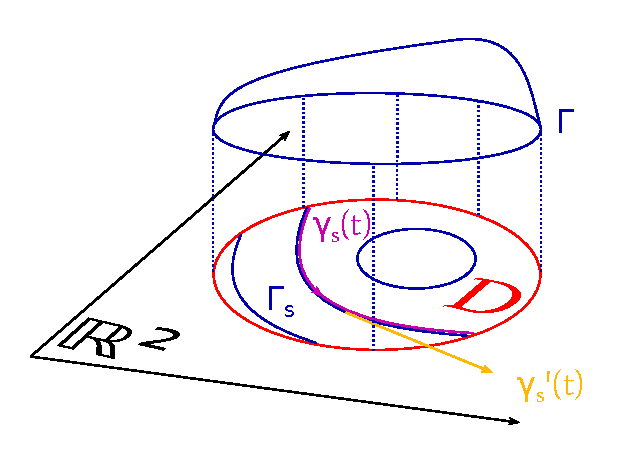
\includegraphics{img/32_niveau.pdf}
      \caption{$\Gamma_S$ is the niveau level of $f$}
      \label{img:niveau}
    \end{center}
  \end{figure}

  Assume $\Gamma_s$ is a graph of a family of curves (dt. \foreignlanguage{german}{Parametrisierte Kurve}) $\gamma_s: I \to D$.
  Let $I$ be an interval. $\Gamma_s = \setdef{\gamma_s(t)}{t \in I}$. We assume, that $\gamma_s$ is regular, hence $\gamma$ is differentiable
  and $\gamma_s'(t) = \begin{bmatrix} \gamma_1'(t) \\ \gamma_2'(t) \end{bmatrix} \neq \begin{bmatrix} 0 \\ 0 \end{bmatrix} \forall t \in I$.
  $\gamma_s'(t)$ is tangential vector on $\Gamma_s$ in point $x = \gamma_s(t)$.

  \[ \angel{\nabla f(\gamma_s(t)), \gamma'_s(t)} = \angel{\nabla f(x), v} = 0 \]
  \[ f(\underbrace{\gamma_s(t)}_{\in \Gamma_s}) = s \qquad \text{\dots constant} \]
  \[ \implies \frac{d}{dt} [f(\gamma_s(t))] = 0  \]
  where
  \begin{align*}
    \frac{d}{dt} f(\gamma_s(t))
      = \underbrace{D f(x)}_{\nabla f(x)^t} \cdot \underbrace{D \gamma_s(x)}_{\gamma_s'(t)}
      &= \nabla f(x)^t \cdot \gamma'_s(t) \\
      &= \angel{\nabla f(x), \gamma'_s(t)}
  \end{align*}
  Compare with Figure~\ref{img:nab}.

  \begin{figure}[!h]
    \begin{center}
      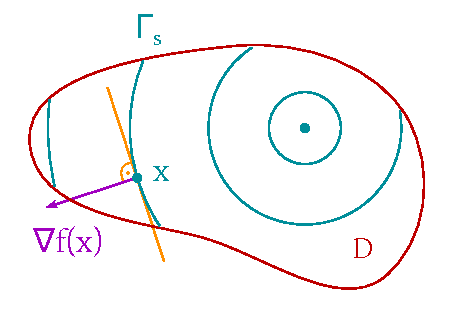
\includegraphics{img/33_gradient_2.pdf}
      \caption{$Df(x) = \nabla f(x)^T$}
      \label{img:nab}
    \end{center}
  \end{figure}
\end{remark}

\begin{theorem} % Satz 2
  \label{thm:rel2}
  This theorem establishes the relation of differentiability and partial derivatives.

  Let $f: D \to \mathbb R$, $D \subseteq \mathbb R^m$ be open.
  Assume all partial derivatives $\partial_i f(x)$ exist $\forall x \in D$ for $j = 1, \dots, m$
  and the functions $x \mapsto \partial_j f(x)$ on $D \to \mathbb R$ are continuous for $j = 1, \dots, m$.
  Then $f$ is differentiable in every point $x_0 \in D$ with $Df(x_0) = [\partial_1 f(x_0), \dots, \partial_m f(x_0)]$.
  Then $f$ is also continuously differentiable.
\end{theorem}

\begin{proof}
  Proof idea: We approximate $x_0$ (starting from $x_0 \in D$) along lines parallel to the coordinate system axes. Compare with Figure~\ref{img:x0xcoord}.

  \begin{figure}[t]
    \begin{center}
      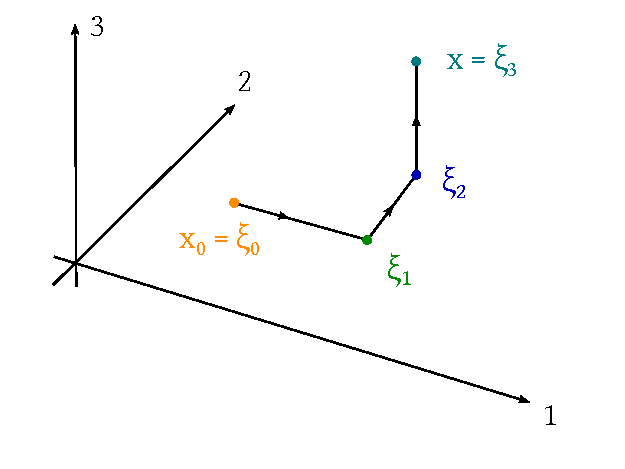
\includegraphics{img/34_axes.pdf}
      \caption{$x_0$ approximates $x$ along lines parallel to the coordinate system axes}
      \label{img:x0xcoord}
    \end{center}
  \end{figure}

  \[
    x_0 \coloneqq \begin{bmatrix} x_1^0 \\ \vdots \\ x_m^0 \end{bmatrix} \qquad
    x \coloneqq \begin{bmatrix} x_1 \\ \vdots \\ x_m \end{bmatrix} \qquad
    \xi_0 \coloneqq x_0 = \begin{bmatrix} x_1^0 \\ x_2^0 \\ \vdots \\ x_m^0 \end{bmatrix} \qquad
    \xi_1 \coloneqq \begin{bmatrix} x_1 \\ x_2^0 \\ \vdots \\ x_m^0 \end{bmatrix} \qquad
    \xi_2 \coloneqq \begin{bmatrix} x_1 \\ x_2 \\ x_3^0 \\ \vdots \\ x_m^0 \end{bmatrix} \qquad
  \] \[
    \xi_k \coloneqq \begin{bmatrix} x_1 \\ \vdots \\ x_{k_0} \\ x_{k+1} \\ \vdots \\ x_m^0 \end{bmatrix} \qquad
    \dots \qquad
    \xi_m \coloneqq \begin{bmatrix} x_0 \\ \vdots \\ x_m \end{bmatrix} = x
  \]
  where $\xi_i$ are \enquote{intermediate} points.
  It holds that $\xi_k + (x_{k+1} - x_{k+1}^0) \cdot e_{k+1} = \xi_{k+1}$ for $k = 0, \dots, m-1$.
  Define $\varphi_k: [0,1] \to \mathbb R$.
  \[ \varphi_k(t) = f(\xi_k + t(x_{k+1} - x_{k+1}^0) \cdot e_{k+1}) \]
  then $\varphi_k(0) = f(\xi_k); \varphi_k(1) = f(\xi_{k+1})$. $\varphi_k'(t) = $?
  \[ \underbrace{f(\xi_k + t(x_{k+1} - x_{k+1}^0) \cdot e_{k+1})}_{= \varphi_k(t)} = f(x_1, \dots, x_k, x_{k+1}^0 + t(x_{k+1} - x_{k+1}^0), x_{k+2}^0, \dots, x_m^0) \]
  \[ \varphi_k'(t) = \frac{d}{dt} \left[f(x_1, \dots, x_k, \underbrace{x_{k+1}^0 + t(x_{k+1} - x_{k+1}^0)}_{(k+1)-\text{th variable}}, x_{k+2}^0, \dots, x_m^0)\right] \]
  \[ = \partial_{k+1} f(x_1, \dots, x_k, x_{k+1}^0 + t(x_{k+1} - x_{k+1}^0), x_{k+2}^0, \dots, x_m^0) \cdot (x_{k+1} - x_{k+1}^0) \]
  \[ = \partial_{k+1} f(\xi_k + t(x_{k+1} + t(x_{k+1} - x_{k+1}^0) \cdot e_{k+1})) \cdot (x_{k+1} - x_{k+1}^0) \]
  $\varphi_k$ is continuously differentiable on $[0,1]$ because $\partial_{k+1} f$ is continuous.
  By the mean value theorem of differential calculus, it follows that some $\tau_{k+1} \in (0,1)$ exists such that
  \[ \varphi(1) - \varphi(0) = \varphi'(\tau_{k+1}) \cdot (1 - 0) \]
  \[ \implies f(\xi_{k+1}) - f(\xi_k) = \partial_{k+1} f(\xi_k + \tau_{k+1}(x_{k+1} - x_{k+1}^0) \cdot e_{k+1}) \cdot (x_{k+1} - x_{k+1}^0) \]
  For differentiability, we have to show:
  \[ \lim_{x\to x_0} \frac{1}{\norm{x - x_0}} \card{f(x) - f(x_0) - [\partial_1 f(x_0), \dots, \partial_m f(x_0)] \begin{bmatrix} x_1 - x_1^0 \\ x_2 - x_2^0 \\ \vdots \\ x_m - x_m^0 \end{bmatrix}} = 0 \qquad (*) \]
  Choose $\norm{x} = \norm{x}_{\infty}$ on $\mathbb R^m$.
  \[ \frac{1}{\norm{x - x_0}} \card{\underbrace{f(x)}_{\xi_m} - \underbrace{f(x_0)}_{\xi_0} - \sum_{k=1}^m \partial_k f(x_0) (x_k - x_k^0)} \]
  \[ = \frac{1}{\norm{x - x_0}} \card{\underbrace{\sum_{k=1}^m (f(\xi_k) - f(\xi_{k-1})}_{\text{telescoping sum}} - \partial_k f(x_0) (x_k - x_k^0))} \]
  \[ \underbrace{\leq}_{\text{triangle ineq.}} \frac{1}{\norm{x - x_0}} \sum_{k=1}^m \card{\partial_k f(\xi_{k-1} + \tau_k (x_k - x_k^0) \cdot e_k) (x_k - x_k^0) - \partial_k f(x_0) (x_k - x_k^0)} \]
  \[ = \sum_{k=1}^m \underbrace{\frac{\card{x_k - x_k^0}}{\norm{x - x_0}}}_{\leq 1} \cdot \card{\partial_k f(\xi_{k-1} + \tau_k(x_k - x_k^0) \cdot e_k) - \partial_k f(x_0)} \qquad (\#) \]
  Choose $\varepsilon > 0$ arbitrary. By continuity of $\partial_k f(x)$, there exists $\delta > 0$ such that $\norm{y - y_0}_{\infty} < \delta \implies \card{\partial_k f(y) - \partial_k f(x_0)} < \frac\varepsilon{m}$ for every $k \in \set{1, \dots, m}$.
  Choose $x$ such that $\norm{x - x_0} \leq \delta$. We consider
  \[
    \xi_{k-1} + \tau_k (x_k - x_k^0) \cdot e_k - x_0
    = \begin{bmatrix} x_1 \\ \vdots \\ x_{k-1} \\ x_k^0 \\ \vdots \\ x_m \end{bmatrix}
    + \begin{bmatrix} 0 \\ \vdots \\ 0 \\ \tau_k(x_k - x_k^0) \\ 0 \\ \vdots \\ 0 \end{bmatrix}
    - \begin{bmatrix} x_1^0 \\ \vdots \\ x_{k-1}^0 \\ x_k^0 \\ \vdots \\ x_m^0 \end{bmatrix}
    = \begin{bmatrix} x_1 - x_1^0 \\ \vdots \\ x_{k-1} - x_{k-1}^0 \\ \tau_k(x_k - x_k^0) \\ 0 \\ \vdots \\ 0 \end{bmatrix}
  \] \[
    \implies
    \norm{\xi_{k-1} + \tau_k (x_k - x_k^0) \cdot e_k - x_0}_{\infty}
  \] \[
    = \max\set{\card{x_1 - x_1^0}, \card{x_2 - x_2^0}, \dots, \card{x_{k-1} - x_{k-1}^0}, \underbrace{\tau_k}_{\in (0,1)} \card{x_k - x_k^0}}
  \] \[
    \leq \norm{x - x_0}_{\infty}
    < \delta
  \] \[
    \implies \card{\partial_k f(\xi_{k-1} + \tau_k (x - x_0^k) e_k) - \delta_k f(x_0)} < \frac\varepsilon{m}
  \] \[
    (\#) \leq 1 \cdot \sum_{k=1}^m \frac\varepsilon m = m \cdot \frac\varepsilon m = \varepsilon
  \]
  Thus, $f$ is differentiable in $x_0$.

  Because $Df(x) = [\partial_1 f(x), \dots, \partial_m f(x)]$ depends continuously on $x$,
  $f$ is continuously differentiable on $D$
\end{proof}

\begin{corollary}
  Let $f: D \subseteq \mathbb R^m \to \mathbb R^n$.
  \[ f(x) = \begin{bmatrix} f_1(x) \\ \vdots \\ f_n(x) \end{bmatrix} \]
  such that all partial derivatives $\partial_k f_i(x)$ exist and are continuous in $x$ (for $k=1,\dots,m$; $i=1,\dots,n$).
  Then $f$ is continuously differentiable on $D$.
\end{corollary}
\begin{proof}[Rationale]
  Use $f$ is continuously differentiable on $D \iff f_i$ is continuously differentiable for $i = 1,\dots,n$ and use Theorem~\ref{thm:rel2}.
\end{proof}

\begin{example}[Counterexample]
  \[
    f(x_1, x_2) = \frac{x_1^2 x_2}{x_1^2 + x_2^2}
    \qquad \partial_1 f(x) = \frac{2x_1 x_2^3}{(x_1^2 + x_2^2)^2}
    \qquad \partial_2 f(x) = \frac{x_1^2 (x_1^2 - x_2^2)}{(x_1^2 + x_2^2)}
  \] \[
    \partial_1 f(0) = \partial_2 f(0) = 0
  \] \[
    \partial_1f(\begin{bmatrix} \varepsilon \\ \varepsilon \end{bmatrix}) = \frac{2 \varepsilon \varepsilon^3}{(\varepsilon^2 + \varepsilon^2)^2} = \frac{2\varepsilon^4}{4 \varepsilon^4} = \frac12 \not\to 0
  \]
  Therefore, $\partial_1 f$ is not continuous in $0$.
\end{example}

\dateref{2018/06/05}

\subsection{Optimality criteria for multi-dimensional functions}

Necessary (but not sufficient) optimality criteria:
\begin{definition} % Definition 7
  Let $D \subseteq \mathbb R^n$, $f: D \to \mathbb R$.
  We say that $f$ in $x_0 \in D$ has a local maximum, if some neighborhood $U$ of $x_0$ exists such that
  \[ \forall x \in D \cap U: f(x) \leq f(x_0) \]
  and accordingly for strict maxima:
  \[ \forall x \in (D \cap U) \setminus \set{x_0}: f(x) < f(x_0) \]
  Analogously for a minimum with $f(x) \geq f(x_0)$ and strict minima $f(x) > f(x_0)$.
\end{definition}

\begin{lemma} % Lemma 8
  \label{l8}
  Let $f: D \to \mathbb R$ be given. Let $D \subseteq \mathbb R^n$ be open.
  Let $x_0 \in D$ be a local maximum or a local minimum and let $f$ in $x_0$ be differentiable.
  Then $Df(x_0) = [0, \dots, 0]$ or $\nabla f(x_0) = \begin{bmatrix} 0 \\ 0 \\ \vdots \\ 0 \end{bmatrix}$.
\end{lemma}

\begin{proof}
  We consider one-dimensional $l_{e_k,x_0}: (-\varepsilon, \varepsilon) \to D$ with $l_{e_k, x_0}(t) \mapsto x_0 + t \cdot e_k$
  and $l_{e_k, x_0}(0) \mapsto x_0$. $f$ has a maximum in $x_0$ (without loss of generality) $\implies f \circ l_{e_k,x_0}$ (differentiable in $t = 0$) is a local maximum in $t = 0$. This is necessary for the optimality of $t = 0$ for $f \circ l_{e_k,x_0}$ that $(f \circ l_{e_k,x_0})'(0) = 0 \implies Df(x_0) \cdot e_k = \partial_k f(x_0) = 0 \implies Df(x_0) = [0, \dots, 0]$.
\end{proof}

\begin{remark}
  By Lemma~\ref{l8} it follows immediately that $x_0$ is optimal.
  \[ \implies \underbrace{Df(x_0)}_{= 0} \cdot v = df(x_0; v) = 0 \qquad \forall v \in \mathbb R^n \]
\end{remark}

\subsection{Diffeomorphism}
\index{Diffeomorphism}
\begin{definition} % Definition 8
  Let $U, V \subseteq \mathbb R^n$ be open.
  We call $f: U \to V$ a \emph{diffeomorphism} if
  \begin{enumerate}
    \item $f: U \to V$ is bijective
    \item $f$ is continuously differentiable on $U$
    \item $f^{-1}: V \to U$ is continuously differentiable on $V$
  \end{enumerate}
  Let $f: U \to V$, $x_0 \in U$ and $y_0 = f(x_0) \in V$.
  We say: $f$ is a local diffeomorphism in $x_0$ if open neighborhoods $x_0 \in U' \subset U$ and $y_0 \in V' \subseteq V$ such that $f: U' \to V'$ is a diffeomorphism.
\end{definition}

\begin{lemma} % Lemma 9
  \label{l9}
  Let $g: D \subseteq \mathbb R^n \to \mathbb R^n$ and $D$ is open.
  $g$ is continuously differentiable on $D$.
  Furthermore let $g: D \to g(D)$ be bijective, $g^{-1}: g(D) \to D$ and $Dg(x)$ is regular for all $x \in D$.
  Then $g(D) \to D$ is continuously differentiable with
  \[ D g^{-1}(y) = Dg^{-1}\left(g(x)\right) = [Dg(x)]^{-1} \]
\end{lemma}

\begin{proof}
  Will be provided later on (page~\pageref{proof:f9}).
\end{proof}

\subsection{Local inversion theorem}
\index{Local Inversion Theorem}
\begin{theorem}[Local Inversion Theorem, Theorem of Inverse Maps]
  \label{thm:lit}
  Let $D \subseteq \mathbb R^n$ be open. Let $f: D \to \mathbb R^n$ be continuously differentiable.
  Furthermore let $Df(x_0)$ be regular for $x_0 \in D$. Then $f$ is a local diffeomorphism in $x_0$.
  Furthermore:
  \[ Df^{-1}(f(x_0)) = [Df(x_0)]^{-1} \]
\end{theorem}
\begin{proof}
  \begin{align*}
    \tilde f(\xi) &= f(\xi + x_0) - f(x_0) \\
    \tilde f: D - x_0 &= \set{\xi = x - x_0: x \in D} \to \mathbb R^n \\
    \tilde f(0) &= f(x_0) - f(x_0) = 0 \\
    D\tilde f(0) &= Df(x_0) \text{ is regular}
  \end{align*}
  \begin{claim}
    $f$ is a local diffeomorphism $\iff \tilde f$ is a local diffeomorphism.
  \end{claim}
  
  \begin{proof}
    \begin{description}
      \item[Direction $\impliedby$]
	    Let $\tilde f$ be a local diffeomorphism.
	    \[ \tilde f(\xi) = \eta \iff \underbrace{f(\xi + x_0)}_{= x} = \underbrace{\eta + f(x_0)}_{y} \iff f(x) = y \]
	    and $\xi = \tilde f^{-1}(\eta)$. Also,
	    \[ x = \xi + x_0 = \tilde f^{-1}(y - f(x_0)) + x_0 \]
	    Thus, $f$ is invertible and
	    \[ f^{-1}(y) = \tilde f^{-1}(y - f(x_0)) + x_0 \]
	    hence $f^{-1}$ is continuously differentiable, hence $f$ is a local diffeomorphism.
	  \item[Direction $\implies$] Analogous.
    \end{description}
  \end{proof}
  \[ F(x) = {\underbrace{[Df(x_0)]}_{\in \mathbb R^{n \times n}}}^{-1} \tilde f(x) \]
  \[ v \mapsto [Df(x_0)]^{-1} \cdot v \text{ linear } \implies \text{ diffeomorphism} \]
  $[Df(x_0)]^{-1} \cdot \tilde f$ is a local diffeomorphism $\iff \tilde f$ is a local diffeomorphism.
  \[ DF(0) = [Df(x_0)]^{-1} \cdot \underbrace{D \tilde f(0)}_{Df(x_0)} = E \]
  Thus, it suffices to show that $F$ is a local diffeomorphism where $F(0) = 0$ and $Df(0) = I$ (the unit matrix).
  
  Now the interesting part of the proof begins:
  Let $y \in \mathbb R^n$ arbitrary. We define
  \[ \varphi(x) = y + x - F(x) \]
  $y = F(x) \iff y + x - F(x) = x$, hence $\varphi_Y(x) = x$, hence $x$ is a fixed point of $\varphi_Y$.
  
  $F$ is continuously differentiable with $DF(0) = I$. Thus for every $\varepsilon > 0 \exists \delta > 0$ such that
  \[ \norm{x - 0} \leq \delta \implies \norm{DF(x) - DF(0)} = \norm{DF(x) - I} \leq \varepsilon \]
  Choose $r > 0$ such that $\norm{x} \leq 2r \implies \norm{DF(x) - I} \leq \frac12$.
  Additionally let $r$ be sufficiently small such that
  \[ \overline{K_{2r}(0)} \subseteq \tilde D = D - x_0 \]
  Recall that $\tilde D$ is the domain of $F$.
  Let $x_1, x_2 \in \overline{K_{2r}(0)}$ and let
  \[ l_{x_1,x_2}: \substack{t \mapsto (1 - t) x_1 + t x_2 \\ [0, 1] \to \overline{K_{2r}(0)}} \]
  
  \begin{figure}[t]
    \begin{center}
      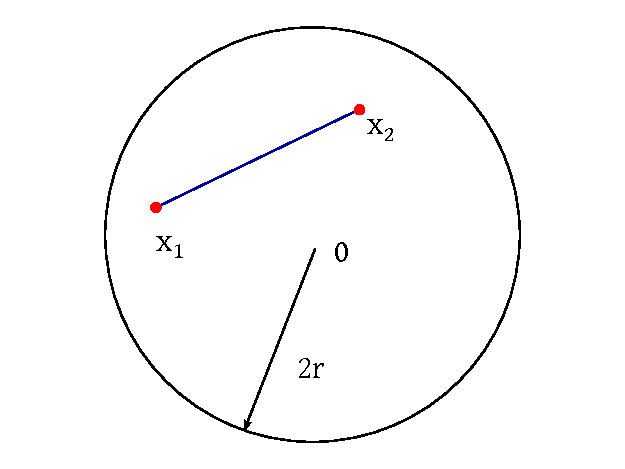
\includegraphics{img/35_x1x2.pdf}
      \caption{We consider a sphere with radius $2r$. The blue line denotes $l_{x_1, x_2}(t)$. $l_{x_1, x_2}(t) \in \overline{K_{2r}(0)}$ because $\overline{K_{2r}(0)}$ is convex}
      \label{img:x1x2}
    \end{center}
  \end{figure}
  
  Compare with Figure~\ref{img:x1x2}.
  \[ l_{x_1 x_2}(0) = x_1 \qquad l_{x_1 x_2}(1) = x_2 \]
  \begin{align*}
	\norm{\varphi_y(x_2) - \varphi_y(x_1)}
	  &= \norm{\varphi_y \circ l_{x_1 x_2}(1) - \varphi_y \circ l_{x_1 x_2}(0)} \\
	  &= \norm{\int_0^1 \frac{d}{dt} [\varphi_Y \circ l_{x_1 x_2}(t)] \, dt} \\
	  &= \norm{\int_0^1 D\varphi_Y(l_{x_1 x_2}(t)) \cdot \underbrace{\left(x_2 - x_1\right)}_{\substack{\text{inner derivative} \\ l_{x_1 x_2}(t)} \, dt}} \\
	  &\leq \int_0^1 \norm{D\varphi_Y(\underbrace{l_{x_1 x_2}(t)}_{\in \overline{K_{2r}(0)}})} \cdot \underbrace{\norm{(x_2 - x_1)}}_{\text{constant}} \, dt \\
	  &\leq (*)
  \end{align*}
  \[ D \varphi_Y(x) = I - DF(x) \]
  hence $\forall x \in \overline{K_{2r}(0)}$, $\norm{D\varphi_Y(x)} = \norm{I - DF(x)} \leq \frac12$.

  \[ (*) \leq \frac12 \norm{x_2 - x_1} \underbrace{\int_0^1 1 \cdot dt}_{= 1} = \frac12 \norm{x_2 - x_1} \]
  Hence $\forall x_1, x_2 \in \overline{K_{2r}(0)}$,
  \[ \norm{\varphi_Y(x_2) - \varphi_Y(x_1)} \leq \frac12 \norm{x_2 - x_2} \]
  Therefore $\varphi_Y$ is a contraction with constant $\nu = \frac12$.

  $K_{2r}(0) \subseteq \mathbb R^n$ is a complete, metric space. It remains to show: $\varphi_Y: \overline{K_{2r}(0)} \to \overline{K_{2r}(0)}$.
  This only holds if $y$ is sufficiently small.
  
  Let $y \in K_r(0)$ and $x \in \overline{K_{2r}(0)}$.
  \begin{align*}
    \norm{\varphi_Y(x)} &= \norm{\varphi_Y(x) - \varphi_Y(0) + \varphi_Y(0)} \leq \norm{\varphi_Y(x) - \varphi_Y(0)} + \norm{\varphi_Y(0)} \\
                        &\underbrace{\leq}_{\text{contraction}} \frac12 \underbrace{\norm{x - 0}}_{\leq 2r} + \underbrace{\norm{y}}_{< r} < 2r
  \end{align*}
  So, for $y \in K_r(0)$ and $x \in \overline{K_{2r}(0)}$, $\varphi_Y(x) \in K_{2r}(0)$.
  By Banach Fixed Point Theorem, there exists a uniquely determined $x$ such that
  \[ x = \varphi_Y(x) \iff y = F(x) \]
  
  Let $U = F^{-1}(K_r(0)) \cap K_{2r}(0)$ where $F^{-1}(K_r(0))$ is open, because $F$ is continuous.
  Hence, $U$ is open and $0 \in U$. Therefore $U$ is an open neighborhood of $0$.

  Show: $F^{-1}: F(U) \to U$ is continuous~\footnote{This proof was added on 2018/06/07 as we initially forgot this condition}:
  Let $x_1 = F^{-1}(y_1), x_2 = F^{-1}(y_2); y_1, y_2 \in F(U)$.
  \[ \varphi_0(x) = x + 0 - F(x) = x - F(x) \]
  \begin{align*}
    x_2 - x_1 &= \underbrace{x_2 - F(x_2)}_{\varphi_0(x_2)} + F(x_2) \underbrace{- x_1 + F(x_1)}_{- \varphi_0(x_1)} - F(x_1) \\
      &= \varphi_0(x_2) - \varphi_0(x_1) + F(x_2) - F(x_1) \\
    \norm{x_2 - x_1} &\leq \norm{\varphi_0(x_2) - \varphi_0(x_1)} + \norm{F(x_2) - F(x_1)} \\
      &\underbrace{\leq}_{\substack{\varphi_0 \text{ is} \\ \text{a contraction}}} \frac12 \norm{x_2 - x_1} + \norm{F(x_2) - F(x_1)}
  \end{align*}
  \[ \norm{F^{-1}(y_2) - F^{-1}(y_1)} \leq 2 \norm{y_2 - y_1} \]
  hence $F^{-1}$ is Lipschitz continuous on $F(U)$, so also continuous.
  
  We show: $DF(x)$ is invertible for all $x \in U$.
  
  Let $v \in \ker(DF(x)) \iff \norm v = \norm{DF(x) \cdot v - v}$ where $DF(x) \cdot v = 0$.
  \[ = \norm{(DF(x) - I) \cdot v} \leq \underbrace{\norm{DF(x) - I}}_{\leq \frac12} \cdot \norm v \leq \frac12 \norm v \]
  \[ \implies \frac12 \norm v \leq 0 \implies \norm v \leq 0 \implies v = 0 \]
  Hence $\ker(DF(x)) = \set{0}$, so $DF(x)$ is regular.
  \[ \forall x \in U = F^{-1}(K_r(0)) \cap K_{2r}(0): y = F(x) \in K_r(0) \]
  On the opposite, $\forall y \in K_r(0)$ there exists some uniquely determined $x \in K_{2r}(0) \cap F^{-1}(K_r(0))$ with $y = F(x)$.
  So $F: U \to K_r(0)$ is bijective and continuously differentiable. Furthermore, $DF(x)$ is regular $\forall x \in U$.
  By Lemma~\ref{l9}, $F$ is a local diffeomorphism in $x = 0$.
  Thus, $f$ is a local diffeomorphism in $x_0$.
  
  So the central idea of this proof was to rewrite $F$ such that we can apply Banach's Fixed Point Theorem.
\end{proof}

\subsection{Implicit functions}
\index{Implicit function}
\begin{theorem}[Implicit function theorem] % Satz 4
  Let $U \subseteq \mathbb R^{n + m} = \mathbb R^n \times \mathbb R^m$.
  $f: U \to \mathbb R^m$ is continuously differentiable.

  \emph{Notation:} $\vectwo xy \in U; x \in \mathbb R^n, y \in \mathbb R^m$. $f\left(\vectwo xy\right) = f(x, y)$.
  
  For $(x_0, y_0) \in U$, $f(x_0, y_0) = 0$.
  Let
  \[
    Df(x_0, y_0) = \begin{bmatrix}
      \partial_{x_1} f_1 & \dots & \partial_{x_n} f_1 & \partial_{y_1} f_1 & \dots & \partial_{y_m} f_1 \\
      \vdots & & \vdots & \vdots & & \vdots \\
      \partial_{x_1} f_m & \dots & \partial_{x_n} f_m & \partial_{y_1} f_m & \dots & \partial_{y_m} f_m
    \end{bmatrix}
  \]
  where the left half is given by $D_x f(x_0, y_0) \in \mathbb R^{m \times n}$ and the right half is given by $D_y f(x_0, y_0) \in \mathbb R^{m \times m}$.
  
  Assumption: Let $D_y f(x_0, y_0)$ be regular.
  
  Then there exists some neighborhood $D$ of $x_0$ in $\mathbb R^n$ and a function $g: D \to E$.
  $E$ is a neighborhood of $y_0$ in $\mathbb R^m$ such that $D \times E \subseteq U$ and $f(x,y) = 0 \iff y = g(x)$ for $(x, y) \in D \times E$.
  Hence, $f(x, g(x)) = 0 \forall x \in D$.
\end{theorem}

\dateref{2018/06/07}

\begin{remark}
  So it holds: $g(x_0) = y_0$.
\end{remark}

\begin{proof}
  \label{proof:ift}
  \[ F: U \subset \mathbb R^{n + m} \to \mathbb R^{n + m} \]
  \[
    F\left(\begin{bmatrix} x \\ y \end{bmatrix}\right)
    = \begin{bmatrix} x \quad (\in \mathbb R^{n}) \\ f(x,y)  \quad (\in \mathbb R^m)\end{bmatrix} \in \mathbb R^{n + m}
  \] \[
    DF\left(\begin{bmatrix} x_0 \\ y_0 \end{bmatrix}\right) = \begin{bmatrix}
      I & 0 \\
      D_x f(x_0, y_0) & D_y f(x_0, y_0)
    \end{bmatrix}
    \in \mathbb R^{(n + m) \times (n + m)}
  \]
  is the Jacobi matrix of $f$.
  \[ \det\left(DF(\vectwo{x_0}{y_0})\right) = \underbrace{\det(I)}_{= 1} \cdot \underbrace{\det(D_yf(x_0, y_0))}_{\neq 0} \neq 0 \]
  so $DF(\vectwo{x_0}{y_0})$ is regular. By the local inversion theorem (Theorem~\ref{thm:lit}), $F$ is a local Diffeomorphism.
  Thus, $\exists V: \vectwo{x_0}{y_0} \in V \subseteq D$ such that $F: V \to F(V)$ is a diffeomorphism.
  $V$ is open, hence $\exists r, r' > 0$ such that
  \[ (x_0, y_0) \in K_r(x_0) \times K_{r'}(y_0) \subseteq V \]
  here $\mathbb R^{n + m}$ is identified as $\mathbb R^n \times \mathbb R^m$.
  \[ F^{-1}: F(V) \to V \qquad F^{-1}(\begin{bmatrix} \xi \\ \eta \end{bmatrix}) = \text{?} \]
  \[ F\vectwo xy = \begin{bmatrix} \xi \\ \eta \end{bmatrix} \iff \begin{bmatrix} x \\ y \end{bmatrix} = F^{-1}(\begin{bmatrix} \xi \\ \eta \end{bmatrix}) \]
  \[ F\vectwo xy = \vectwo{x}{f(x,y)} \]
  hence $x = \xi$ and $F^{-1}(\begin{bmatrix} \xi \\ \eta \end{bmatrix}) = \begin{bmatrix} \xi \\ G(\xi, \eta) \end{bmatrix}$.
  Define $g(x) \coloneqq G(x, 0)$. $g: K_r(x_0) \to \mathbb R^m$.
  \[ \begin{bmatrix} x \\ 0 \end{bmatrix} = F\left(F^{-1}\left(\begin{bmatrix} x \\ 0 \end{bmatrix}\right)\right) = F\left(\begin{bmatrix} x \\ G(x, 0) \end{bmatrix}\right) = F\left(\begin{bmatrix} x \\ g(x) \end{bmatrix}\right) = \begin{bmatrix} x \\ f(x, g(x)) \end{bmatrix} \]
  \[ \implies f(x, g(x)) = 0 \forall x \in K_r(x_0) \]
  Uniqueness: Let $(x, y) \in K_r(x_0) \times K_{r'}(y_0) \subset V$ and $f(x, y) = 0$.
  Hence
  \[ F(\begin{bmatrix} x \\ y \end{bmatrix}) = \begin{bmatrix} x \\ f(x, y) \end{bmatrix} = \begin{bmatrix} x \\ 0 \end{bmatrix} \]
  \[ \implies \begin{bmatrix} xy \end{bmatrix} = F^{-1}(F(\begin{bmatrix} x \\ y \end{bmatrix})) = F^{-1}(\begin{bmatrix} x \\ 0 \end{bmatrix}) = \begin{bmatrix} x \\ G(x,0) \end{bmatrix} = \begin{bmatrix} x \\ g(x) \end{bmatrix} \]
  \[ \implies y = g(x) \]
\end{proof}

\begin{example}
  \[ f(x, y) = x^2 y - x^3 y^2 - 2 \]
  \[ f(-1, 1) = 1 + 1 - 2 = 0 \]
  Hence $(x_0, y_0) = (-1, 1)$ is root of $F$.
  \[ Df(x, y) = \left[\underbrace{2xy - 3x^2 y^2}_{D_x f}, \underbrace{x^2 - 2x^3 y}_{D_y f}\right] \]
  \[ D_y f(\begin{bmatrix} -1 \\ 1 \end{bmatrix}) = 3 \neq 0 \]
  hence $f(x, y)$ is in neighborhood of $(-1, 1)$ resolvable by $y$.
  \[ x^2 y - x^3 y^2 - 2 = 0 \]
  \[ x^3 y^2 - x^2 y + 2 = 0 \]
  \[ y = \frac{x^2 \pm \sqrt{x^4 - 8x^3}}{2x^3} = \frac{x^2 (1 \pm \sqrt{1 - \frac{8}{x}})}{2x^3} = \frac{1}{2x} \left(1 \pm \sqrt{1 - \frac8x}\right) \]
  It has to holds that $g(-1) = 1$, thus
  \[ \frac1{-2} \left(1 + \sqrt{1 - \frac{8}{-1}}\right) = -\frac12 (1 + 3) = -2 \]
  This is apparently wrong, thus we consider the second result for $y$:
  \[ \frac1{-2} \left(1 - \sqrt{1 - \frac{8}{-1}}\right) = -\frac12 (1 - 3) = -1 \]
  So $g(x) = \frac1{2x} \cdot \left(1 - \sqrt{1 - \frac8x}\right)$ is the desired function.
  $D_x f(-1, 1) = -2 - 3 = -5$, hence $f(x, y) = -x^3 y^2 + x^2 y - 2$ is also uniquely resolvable by $x$ in a neighborhood of $(-1, 1)$.
\end{example}

\begin{proof}[Proof of Lemma~\ref{l9}]
  \label{proof:f9}
  Choose $x_0 \in D$ and show that $g^{-1}$ is differentiable in $y_0 = g(x_0)$.
  We use the same construction as in Proof~\ref{proof:ift} (Implicit function theorem proof).
  Without loss of generality: $x_0 = 0; g(x_0) = y_0 = 0$ and $Dg(0) = I$.
  Let $v \in \mathbb R^n$ be sufficiently small such that $w = g^{-1}(v)$ is defined.

  By differentiability of $g$,
  \[ g(w) = \underbrace{Dg(0)}_{I} \cdot w + \underbrace{R(w)}_{o(\norm{w})} = w + R(w) \]
  \[ g^{-1}(v) = w = g(w) - R(w) = g(g^{-1}(v)) - R(g^{-1}(v)) = v + R^{*}(v) \]
  with $R^{*}(v) = -R(g^{-1}(v))$. Show that $R^*(v) = o(\norm{v})$.
  \begin{align}
    g^{-1}(v) &= v + R^{*}(v)  \label{h}
  \end{align}

  By differentiability of $g$,
  \[ \exists r > 0: \norm{R(w)} \leq \frac12 \norm{w} \]
  for all $\norm{w} \leq r$ (because $\frac{\norm{R(w)}}{\norm{w}} \to 0$ for $w \to 0$).
  Continuity of $g^{-1}$ combined with $g^{-1}(0) = 0$
  \[ \implies \forall \norm{v} < \delta: \norm{g^{-1}(v)} = \norm{g^{-1}(v) - g^{-1}(0)} \leq r \]
  \[ \implies \norm{R^*(v)} = \norm{R(g^{-1}(v))} \leq \frac12 \norm{g^{-1}(v)} \]
  for all $v$ with $\norm{v} \leq \delta$.

  By Equation~\eqref{h},
  \[ \norm{g^{-1}(v)} = \norm{v + R^*(v)} \leq \norm v + \norm{R^*(v)} \leq \norm v + \frac12 \norm{g^{-1}(v)} \]
  If $\norm v \leq \delta$
  \[ \norm{g^{-1}(v)} \leq 2 \norm v \qquad \forall \norm v \leq \delta \]
  So,
  \[ \frac{\norm{R^*(v)}}{\norm{v}} \leq 2 \frac{\norm{R(g^{-1}(v))}}{\norm{g^{-1}(v)}} = 2 \frac{\norm{R(w)}}{\norm{w}} \]
  \[ v \to 0 \implies w = g^{-1}(v) \to 0 \]
  because $g^{-1}$ is continuous, hence
  \[ v \to 0: \lim_{v \to 0} \frac{\norm{R(g^{-1}(v))}}{\norm{g^{-1}(v)}} = \lim_{w \to 0} \frac{R(w)}{\norm{w}} = 0 \]
  because $R = o(\norm{w})$. Thus, $R^*(v) = o(\norm v)$, so $g^{-1}$ is differentiable in $y_0 = 0$.

  We know that $g^{-1}$ is differentiable in every point $y \in g(D)$.
  \[ \underbrace{y}_{= \operatorname{id}(y)} = g(g^{-1}(y)) \forall y \in E = g(D) \]
  We derive both sides of the equation and apply the chain rule:
  \[ D\operatorname{id}(y) = I = Dg(g^{-1}(y)) \cdot Dg^{-1}(y) \]
  \[ \implies Dg^{-1}(y) = [\underbrace{Dg(\underbrace{g^{-1}(y)}_{\text{continuous}} )}_{\text{continuous}}]^{-1} \]
  Is the inverse also continuous (does the inverse depend continuously on the coefficients? Yes, you can see it by considering Cramer's Rule which provides a formula with a sum)? So the inverse is a continuous operation on $\operatorname{GL}(n)$.
  Therefore $Dg^{-1}(y)$ depends continuously on $y$ and $Dg^{-1}(y) = [Dg(x)]^{-1}$ with $x = g^{-1}(y)$ and accordingly, $y = g(x)$.
\end{proof}

\subsection{Higher partial derivatives and multi-dimensional Taylor Theorem}

\index{Order of a partial derivative}
\begin{remark}[Concept idea]
  Let $D \subseteq \mathbb R^n$ be open. Let $f: D \to \mathbb  R$ be continuously differentiable.
  Hence $\partial_{x_i} f(x) \in \mathbb R$ and $\partial_{x_i} f: D \to \mathbb R$ is continuous.
  If $\partial_{x_i} f$ is also (continuously) differentiable, then its partial derivatives can be determined.
  In this case, we define
  \[ \partial_{X_j, X_i} f \coloneqq \partial_{X_j} [\partial_{X_i} f] \]
  Continuation for further higher derivatives:
  \[ \partial_{X_{i_k}, X_{i_{k-1}}, \dots, X_{i_1}} f = \partial_{X_{i_k}} (\partial_{X_{i_{k-1}} \dots X_{i_1}} f) \]
  The index $k$ in $\partial_{X_{i_k} X_{i_{k-1}} \dots X_{i_1}}$ is the \emph{order of the partial derivative}.
\end{remark}

\begin{example}
  \begin{align*}
    f(x, y) &= x^2 y - x^3 y^2 - 2 \\
    \partial_X f &= 2xy - 3x^2 y^2 \\
    \partial_Y f &= x^2 - 2x^3 y \\
    \partial_{YX} f &= 2x - 6x^2y \\
    \partial_{XY} f &= 2x - 6x^2y = \partial_{YX} \\
    \partial_{XX} f &= 2y - 6xy^2 \\
    \partial_{YY} f &= -2x^3 \\
    \partial_{XXX} f &= -6y^2 \\
    \partial_{YYY} f &= 0 \\
    \partial_{XYX} f &= 2 - 12xy \\
    \partial_{XXY} f &= 2 - 12xy = \partial_{XYX} \\
    \partial_{YXY} f &= -6x^2 \\
    \partial_{XYY} f &= -6x^2 = \partial_{YXY} \\
  \end{align*}
  It seems that the derivative is independent of the order of the variables.
\end{example}

\index{Hessian matrix}
\begin{definition}[Hesse matrix]
  Specifically for second derivatives:
  \[
    D^2 f(x) = \begin{bmatrix}
      \partial_{X_1,X_1} f & \partial_{X_2,X_1} f & \dots & \partial_{X_n,X_1} f \\
      \partial_{X_1,X_2} f & \partial_{X_2,X_2} f & \dots & \partial_{X_n,X_2} f \\
      \vdots & \vdots & \ddots & \vdots \\
      \partial_{X_1,X_n} f & \partial_{X_2,X_n} f & \dots & \partial_{X_n,X_n} f
    \end{bmatrix}
  \]
  is called \emph{Hessian matrix}. Named after Otto Hesse (1811--1874).
\end{definition}

\index{$k$-times continuously differentiable}
\begin{definition}
  Let $f: D \to \mathbb R$ and let all partial derivatives of $f$ up to order $k \in \mathbb N$ exist and be continuous functions in $x \in D$.
  Then $f$ is called \emph{$k$-times continuously differentiable} and
  \[ \mathcal C^k(D) \coloneqq \set{f: D \to \mathbb R: f \text{ is $k$-times continuously differentiable}} \]
  $\mathcal C^k(D)$ is a vector space.
\end{definition}

\begin{remark}
  Hermann Amadeus Schwarz (1843--1921)
\end{remark}

\index{Symmetry of second derivatives}
\index{Schwarz' theorem}
\index{Clairaut's theorem}
\index{Young's theorem}
\begin{theorem}[Symmetry of second derivatives, Schwarz' theorem, Clairaut's theorem, Young's theorem] % Satz 5
  Let $f \in \mathcal C^2(D)$. Let $D \subseteq \mathbb R^n$ be open. Then,
  \[ \partial_{X_i X_j} f = \partial_{X_j X_i} f \text{ on } D \]
\end{theorem}

\dateref{2018/06/12}

\begin{proof}
  Let $x_0 \in D$ and $\overline{K_r(x_0)} \subseteq D$. Let $h, k \in \mathbb R$ with $\card{h} \leq \frac r2$ and $\card{k} \leq \frac r2$.
  So $x_0 + h e_i \in \overline{K_{\frac r2}(x_0)}$ and $x_0 + ke_j \in \overline{K_{\frac r2}(x_0)}$ and also
  $x_0 + he_i + ke_j \in \overline{K_r(x_0)}$, because
  \[ \norm{x_0 + he_i + ke_j - x_0} \leq \card{h} \norm{e_i} + \card{k} \norm{e_j} = \card{h} + \card{k} \leq \frac r2 + \frac r2 = r \]
  \[ F: \left[-\frac r2, \frac r2\right] \times \left[-\frac r2, \frac r2\right] \to \mathbb R \]
  \[ F(h, k) \coloneqq f(x_0 + he_i + ke_j) - f(x_0 + he_i) - f(x_0 + ke_j) + f(x_0) \]
  \[ \varphi: \left[-\frac r2, \frac r2\right] \to \mathbb R \qquad \text{$k$ fixed}  \]
  \[ \varphi(\lambda) \coloneqq f(x_0 + \lambda e_i + ke_j) - f(x_0 + \lambda e_i) \]
  \[ \implies \varphi(0) = f(x_0 + ke_j) - f(x_0) \]
  \[ \varphi(h) = f(x_0 + he_i + ke_j) - f(x_0 + he_i) \]
  Therefore, $F(h, k) = \varphi(h) - \varphi(0)$.
  $\varphi$ is continuously differentiable (because $f \in \mathcal C^2$).
  By the Mean Value Theorem of Differential Calculus:
  \[ \exists \lambda \in (-h, h): F(h, k) = \varphi(h) - \varphi(0) = \int_0^h \varphi'(x) \cdot 1 \, dx = \varphi'(\lambda) \cdot (h - 0) = \varphi'(\lambda) \cdot h \]
  and accordingly $\card{\lambda} < \card{h}$.
  \[ \varphi'(\lambda) \cdot h = h \cdot [Df(x_0 + \lambda e_i + ke_j) \cdot e_i - Df(x_0 + \lambda e_i) \cdot e_i] \]
  \[ Df \cdot e_i = \partial_{x_i} f \]
  and also 
  \[ \varphi'(\lambda) \cdot h = h \cdot [\partial_{x_i} f(x_0 + \lambda e_i + k \cdot e_j) - \partial_{x_i} f (x_0 + \lambda e_i)] \]
  \[ \partial_{x_i} f \text{ is continuously differentiable} \]
  \[ \psi(\mu) = \partial_{x_i} f(x_0 + \lambda e_i + \mu e_j) \text{ is continuously differentiable} \]
  So we apply the Mean Value Theorem:
  \[ F(h,k) = \varphi'(\lambda) \cdot h = h [\psi(k) - \psi(0)] \]
  \[ h \cdot k \cdot \psi'(\mu) \text{ with appropriate } \mu \in \left[-\card{k}, \card{k}\right] \]
  \[ \psi'(\mu) = \partial_{x_j x_i} f(x_0 + \lambda e_i + \mu e_j) \]
  \[ \implies \exists (\lambda, \mu) \in \left[-\card{h}, \card{h}\right] \times \left[-\card{k}, \card{k}\right] \text{ such that} \]
  \[ {\color{blue} F(h, k)} = h \cdot k \cdot \partial_{x_j x_i} f(x_0 + \lambda e_i + \mu e_j) \]
  Analogously,
  \[ \tilde \varphi(\eta) = f(x_0 + he_i + \eta e_j) - f(x_0 + \eta e_j) \]
  \[ \text{like above: } F(h,k) = \tilde \varphi(k) - \tilde \varphi(0) = k\tilde \varphi'(\eta) \]
  with appropriate $\eta \in \left[-\card{k}, \card{k}\right]$.
  \[ k \tilde \varphi'(\eta) = k \left[\partial_{x_j} f(x_0 + he_i + \eta e_j) - \partial_{x_j} f(x_0 + \eta e_j)\right] \]
  \[ \tilde \psi(\xi) = \partial_{x_j} f(x_0 + \xi e_i + \eta e_j) \text{ and Mean Value Theorem} \]
  \[ \implies {\color{red} F(h, k)} = k \cdot h \cdot \partial_{x_i x_j} f(x_0 + \xi e_i + \eta e_j) \]
  with $(\xi, \eta) \in [-\card{h}, \card{h}] \times [-\card{k}, \card{k}]$.

  Because ${\color{blue} F(h, k)} = {\color{red} F(h, k)}$,
  \begin{align*}
    hk \cdot \partial_{x_j x_i} f(x_0 + \lambda e_i + \mu e_j) &= kh \cdot \partial_{x_i x_j} f(x_0 + \xi e_i + \mu e_j) \\
    \implies \partial_{x_i x_j} f(x_0 + \lambda e_i + \mu e_j) &= \partial_{x_j x_i} f(x_0 + \xi e_i + \eta e_j)
  \end{align*}
  with $\card{\lambda} < \card{h}, \card{\xi} < \card{h}$ and $\card{\mu} < \card{k}, \card{\eta} < \card{k}$.
  $h \to 0, k \to 0 \implies \lambda \to 0, \mu \to 0, \xi \to 0, \eta \to 0$.
  \[ f \in \mathcal C^2 \implies \partial_{x_i x_j} f \text{ and } \partial_{x_j x_i} f \text{ are continuous} \]
  \[
    \implies \partial_{x_j x_i} f(x_0) = \lim_{\lambda, \mu \to 0} \partial_{x_j x_i} f(x_0 + \lambda e_i + \mu e_j)
    = \lim_{\xi,\eta \to 0} \partial_{x_i x_j} f(x_0 + \xi e_i + \eta e_j) = \partial_{x_i x_j} f(x_0)
  \]
  Counterexample:
  \[
    f(x_1, x_2) = \begin{cases}
      \frac{x_1 x_2 (x_1^2 - x_2^2)}{x_1^2 + x_2^2} & \text{ for } (x_1, x_2) \neq (0, 0) \\
      0 & \text{ for } (x_1, x_2) = 0
    \end{cases}
  \]
  here it holds that $\partial_{x_1 x_2} f(0, 0) \neq \partial_{x_2 x_1} f(0, 0)$.
\end{proof}

\begin{theorem}[Generalization of Schwarz' Theorem]
  Let $f \in \mathcal C^k(D)$, $D \subseteq \mathbb R^n$ open and $x_0 \in D$.
  Let $(i_1, i_2, \dots, i_k) \in \underbrace{\set{1,2, \dots, n}^k}_{M_n} = M_n^k$.
  Furthermore let $(i_1', i_2', \dots, i_k')$ be a rearrangement of $(i_1, i_2, \dots, i_k)$.
  Then
  \[ \partial{x_{i_1} x_{i_2} \dots x_{i_k}} f(x_0) = \partial_{x_{i'_1} x_{i'_2} \dots x_{i'_k}} f(x_0) \]
\end{theorem}

\begin{proof}
  Proof by complete induction.
  \index{Multiindex notation}
  \begin{definition}[Multiindex notation] % Definition 9
    Let $I \in \mathbb N^n$, $I = (\alpha_1, \alpha_2, \dots, \alpha_n)$.
    $\alpha_i \geq 0$. We call $I$ a multiindex $k = \card{I} = \sum_{i=1}^n \alpha_i$ is the \emph{order of $I$}.
    \[ \partial_{\underbrace{x_i x_i \dots x_i}_{\alpha \text{ times}}} \eqqcolon \partial_{x_i}^\alpha \]
    is called \emph{$\alpha$-times partial derivative to variable $x_i$}.
    By convention,
    \[ \partial_{x_i}^0 = f \]

    We let
    \[ \partial_I f = \partial_{x_1}^{\alpha_1} \partial_{x_2}^{\alpha_2} \dots \partial_{x_n}^{\alpha_n} f \]
    Furthermore, we use
    \[ \partial_{i_1, i_2, \dots, i_k} \text{ for } \partial_{x_{i_1} x_{i_2} \dots x_{i_k}} \]
    hence
    \[ \underbrace{\partial_{1312}}_{\text{no parentheses}} f = \partial_{x_1 x_3 x_1 x_2} f = \underbrace{\partial_{(2, 1, 1)}}_{\substack{\text{multiindex} \\ \text{with parentheses}}} f \]
    Furthermore we let $I! = \alpha_1! \alpha_2! \dots \alpha_n! = \prod_{i=1}^n \alpha_i!$
    and for $v \in \mathbb R^n: v = [v_1, v_2, \dots, v_n]^T$ we write
    \[ v^I = \alpha_1^{\alpha_1} v_2^{\alpha_2} \dots v_n^{\alpha_n} = \prod_{i=1}^n v_i^{\alpha_i} \]
  \end{definition}

  The proof is left as an exercise to the reader.
\end{proof}

\index{Taylor's theorem in the multidimensional case}
\begin{theorem}[Multidimensional Taylor's theorem] % Satz 6
  \label{multiTaylor}
  Let $f: D \to \mathbb R$. $D$ is open. Let $x_0 \in D$ and $f \in \mathcal C^{k+1}(D)$.
  Let $r > 0$ such that $K_r(x_0) \subseteq D$ and $v \in \mathbb R^n$ with $\norm{v} \leq r$
  (hence, $x_0 + v \in \overline{K_r(x_0)}$ and therefore also the connecting line
  $[x_0, x_0 + v] = \set{x_0 + tv: t \in [0, 1]} \subseteq \overline{K_r(x_0)} \subseteq D$).
  Then there exists $\vartheta \in (0,1)$ such that
  \begin{align*}
    f(x_0 + v) &= \underbrace{f(x_0) + \sum_{j=1}^k \frac1{j!} \sum_{i_1, i_2, \dots, i_j=1}^{n} \partial_{i_1 i_2 \dots i_j} f(x_0) \cdot v_{i_1} \cdot v_{i_2} \cdots v_{i_j}}_{T_f^k(x_0 + v; x_0)} \\
      &+ \underbrace{\frac{1}{(k+1)!} \sum_{i_1 i_2 \dots i_{k+1} = 1}^n \partial_{i_1 i_2 \dots i_{k+1}} f(x_0 + \vartheta v) v_{i_1} v_{i_2} \dots v_{i_{k+1}}}_{R_f^{k+1}(x_0 + v; x_0)}
  \end{align*}
  where $T_f^k(x_0 + v; x_0)$ is the Taylor polynomial of $k$-th order and $R_f^{k+1}(x_0 + v; x_0)$ is the remainder term.
  But in this notation some terms occur multiple times. For example, $\partial_{1121} = \partial_{2111}$. Alternatively,
  \[ f(x_0 + v) = f(x_0) + \sum_{j=1}^k \sum_{\card{I} = j} \frac{1}{I!} \partial_I f(x_0) \cdot v^I + \sum_{\card{I} = k+1} \frac{1}{I!} \partial_I f(x_0 + \vartheta v) \cdot v^I  \]
\end{theorem}

\begin{proof}
  Consider $\varphi: [0,1] \to \mathbb R$.
  \[ \varphi(t) = f(x_0 + tv) = f \circ l_{x_0,v}(t) \]
  \[ f \in \mathcal C^{(k+1)}(D) \implies \varphi \in \mathcal C^{(k+1)}([0,1]) \]
  \begin{claim}
    \[ \varphi^{(j)}(t) = \sum_{i_1,i_2,\dots,i_j=1}^n \partial_{i_1 i_2 \dots i_j} f(x_0 + tv) \]
  \end{claim}
  \begin{proof}
    Proof by induction over $j$.
    \begin{description}
      \item[Induction base $j = 0$]
        \begin{align*}
          \varphi(t) &= f \circ l_{x_0,v}(t) \\
          \varphi'(t) &\underbrace{=}_{\substack{\text{chain} \\ \text{rule}}} Df(x_0 + \underbrace{t}_{\substack{\text{Jacobi matrix} \\ \text{row vector}}}v) \cdot v \\
            &= [\partial_1 f(x_0 + tv), \partial_2 f(x_0 + tv), \dots, \partial_n f(x_0 + tv)]\begin{bmatrix} v_1 \\ \vdots \\ v_n \end{bmatrix} \\
            &= \sum_{i_1=1}^n \partial_{i_1} f(x_0 + tv) \cdot v_{i_1}
        \end{align*}
      \item[Induction step $j-1 \mapsto j$]
        \begin{align*}
          \varphi^{(j)}(t)
            &= (\varphi^{(j-1)})'(t) \\
            &\underbrace{=}_{\substack{\text{induction} \\ \text{hypothesis}}} \frac{d}{dt} \left[\sum_{i_1,i_2,\dots,i_{j-1}=1}^n \underbrace{\partial_{i_1,\dots,i_{j-1}} f(x_0 + tv)}_{\partial_{i_1,\dots,i_{j-1}} f \circ l_{x_0,v}(t)} v_{i_1} \cdot \dots \cdot v_{i_{j-1}} \right] \\
            &= \sum_{i_1,\dots,i_j = 1}^n \partial_{i_1, \dots, i_j} f(x_0 + tv) v_{i_1} \dots v_{ij}
        \end{align*}
    \end{description}
  \end{proof}
  Taylor's Theorem for $\varphi(1)$ in the 1-dimensional case:
  \[ \varphi(1) = \varphi(0) + \sum_{j=1}^n \frac{1}{j!} \varphi^{(j)}(0) \cdot 1^j + \frac{1}{(k+1)!} \varphi (\vartheta) \cdot 1 \]
  with $\vartheta \in (0,1)$.
  Insertion:
  \[ f(x_0 + v) = f(x_0) + \sum_{j=1}^n \frac{1}{j!} \sum_{i_1,\dots,i_j=1}^n \partial_{i_1,\dots,i_j} f(x_0) v_{i_1} \dots v_{i_j} \]
  \[ + \frac{1}{(k+1)!} \sum_{i_1 \dots i_{k+1}=1}^n \partial_{i_1 \dots i_{k+1}} f(x_0 + \vartheta v) \cdot v_{i_1} v_{i_2} \dots v_{i_{k+1}} \]

  Alternative notation with multiindices:
  \[ \partial_{i_1 i_2 \dots i_j} f(x_0) = \partial_{i'_1 i'_2 \dots i'_j} f(x_0) \]
  if $i_1 i_2 \dots i_j$ and $i_1' i_2' \dots i_j'$ only distinguish by the order of indices.
  How many ways are there to put indices in order?

  Let $I = (\alpha_1, \alpha_2, \dots, \alpha_n)$ be a multiindex
  \[ \partial_I = \partial_{(\alpha_1,\alpha_2,\dots,\alpha_n)} = \partial_{\underbrace{11\dots 1}_{\alpha_1-\text{times}}} \overbrace{2 \dots 2}^{\alpha_2-\text{times}} \underbrace{3 3 \dots 3}_{\alpha_3-\text{times}} \dots \overbrace{n n \dots n}^{\alpha_n-\text{times}} \]
  How many ways are there to distribute
  \[ \underbrace{\underbrace{1 1 \dots 1}_{\alpha_1} \overbrace{2 2 \dots 2}^{\alpha_2} \underbrace{3 3 \dots 3}_{\alpha_3} \dots \overbrace{n n \dots n}^{\alpha_n}}_{j} \]
  is different order?
  There are ${j \choose \alpha_1}$ different ways to distribute one.
  There are ${j-\alpha_1 \choose \alpha_2}$ different ways to distribute two.
  There are ${j-\alpha_1-\alpha_2 \choose \alpha_3}$ different ways to distribute three.
  And so on. There ${j-\alpha_1-\alpha_2-\dots-\alpha_{n-1} \choose \alpha_n}$ different ways to distribute $n$.
  \begin{align}
    \begin{bmatrix} j \\ \alpha_1 \end{bmatrix} \begin{bmatrix} j-\alpha_1 \\ \alpha_2 \end{bmatrix} \begin{bmatrix} j-(\alpha_1 + \alpha_2) \\ \alpha_3 \end{bmatrix} \dots \begin{bmatrix} j-(\alpha_1 + \dots + \alpha_{n-1}) \\ \alpha_n \end{bmatrix} \label{arr}
  \end{align}
  are different arrangements of the index list.
  \[ \underbrace{1 1 \dots 1}_{\alpha_1} \overbrace{2 \dots 2}^{\alpha_2} \dots \underbrace{n n \dots n}_{\alpha_n} \]
  \begin{align*}
    \eqref{arr} &=
      \frac{j!}{\alpha_1!(j-\alpha_1)!}
      \frac{(j-\alpha_1)!}{\alpha_2! (j - (\alpha_1 + \alpha_2))!}
      \frac{(j-(\alpha_1 + \alpha_2))!}{\alpha_3! (j - (\alpha_1 + \alpha_2 + \alpha_3))!} \\
      &\dots
      \frac{(j - (\alpha_1 + \dots, \alpha_{n-1}))!}{\alpha_n! \underbrace{(j - \underbrace{(\alpha_1 + \dots + \alpha_n)}_{=j})!}_{= 0! = 1}} \\
      &= \frac{j!}{\alpha_1! \alpha_2! \dots \alpha_n!}
  \end{align*}

  We merge equal partial derivative
  \begin{align*}
    f(x_0 + v) &= f(x_0) + \sum_{j=1}^k \frac{1}{j!} \sum_{\card{I}=j}  \frac{j!}{I!} \cdot \partial_I f(x_0) \cdot v^I \\
      &+ \sum_{\card{I} = k+1} \frac{1}{(k+1)!} \cdot \frac{(k+1)!}{I!} \cdot \partial_I f(x_0 + \vartheta v) v^I
  \end{align*}
\end{proof}

\begin{example}
  \[ f: \mathbb R^2 \to \mathbb R \text{ arbitrarily often differentiable} \]
  \begin{align*}
    f(x_0 + v) &= f(x_0) + \partial_1 f(x_0) \cdot v_1 + \partial_2 f(x_0) v_2 \\
      &+ \frac1{2!} \partial_{11} f(x_0) v_1 v_1 + \frac{1}{2!} \partial_{12} f(x_0) v_1 v_2 \\
      &+ \frac{1}{2!} \partial_{21} f(x_0) v_2 v_1 + \frac{1}{2!} \partial_{22} f(x_0) v_2 v_2 \\
      &+ \frac{1}{3!} \partial_{111} f(x_0) v_1 v_1 v_1 + \frac{1}{3!} \partial_{211} f(x_0) v_2 v_1 v_1 + \\
      &+ \frac{1}{3!} \partial_{121} f(x_0) v_1 v_2 v_1 + \frac{1}{3!} \partial_{112} f(x_0) v_1 v_1 v_2 + \\
      &+ \frac{1}{3!} \partial_{122} f(x_0) v_1 v_2 v_2 + \frac{1}{3!} \partial_{212} f(x_0) v_2 v_1 v_2 + \\
      &+ \frac{1}{3!} \partial_{221} f(x_0) v_2 v_2 v_1 + \frac{1}{3!} \partial_{222} f(x_0) v_2 v_2 v_2 + R \\
      &= f(x_0) + \partial_{(1,0)} f(x_0) \cdot v_1^1 v_2^0 + \partial_{(0,1)} f(x_0) v_1^0 v_2^1 \\
      &+ \frac{1}{2! 0!} \partial_{(2,0)} f(x_0) v_1^2 v_2^0 + \frac{1}{1! 1!} \partial_{(1,1)} f(x_0) v_1^1 v_2^1 \\
      &+ \frac{1}{0! 2!} \partial_{(0,2)} f(x_0) v_1^0 v_2^2 + \frac{1}{3! 0!} \partial_{(3,0)} f(x_0) v_1^3 v_2^0 \\
      &+ \frac{1}{2! 1!} \partial_{(2,1)} f(x_0) v_1^2 v_2^1 + \frac{1}{1! 2!} \partial_{(1,2)} f(x_0) v_1^1 v_2^2 \\
      &+ \frac{1}{0! 3!} \partial_{(0,3)} f(x_0) v_1^0 v_2^3 + R
  \end{align*}
\end{example}

\dateref{2018/06/14}

\begin{theorem}[Qualitative Taylor Theorem] % Satz 7
  Let $f \in \mathcal C^k(D)$, $D \subseteq \mathbb R^n$ open, $x_0 \in D$.
  Let $r > 0$ such that $K_r(x_0) \subseteq D$ and $\norm{v} < r$, hence $x_0 + v \in K_r(x_0) \subseteq D$.
  Then
  \[ f(x) = \sum_{j=0}^k \sum_{\card{I} = j} \frac{1}{I!} \partial_I f(x_0) v^I + o(\norm{v})^k \]

  Pay attention to $\mathcal C^k(D)$, $j=0$ and $o(\norm{v})^k$.
\end{theorem}

\begin{proof}
  Use the $1$-norm $\norm{v}_1 = \sum_{i=1}^n \card{v_i}$ for the proof. By the equivalence of norms in $\mathbb R^n$, it holds for every norm in $\mathbb R^n$.
  \begin{align*}
    \norm{v}_1^k &= \left(\sum_{k=1}^n \card{v_i}\right)^k \underbrace{=}_{\text{Theorem~\ref{multiTaylor}}}
                    \sum_{\card{I} = k} \frac{k!}{I!} \card{v^I}
  \end{align*}
  for every multiindex $I$ of order $k$, $\frac{1}{I!} \card{v^I} \leq \frac{1}{k!} \norm{v}_1^k$.
  By Theorem~\ref{multiTaylor},
  \begin{align*}
    f(x) &= \sum_{j=0}^{k-1} \sum_{\card{I}=j} \frac{1}{I!} \partial_I f(x_0) v^I {\color{gray} + \sum_{\card{I} = k} \frac{1}{I!} \partial_I f(x_0) v^I} \\
         &+ \sum_{\card{I} = k} \frac{1}{I!} \partial_I f(x_0 + \vartheta v) \cdot V^I {\color{gray} - \sum_{\card{I} = k} \frac{1}{I!} \partial_I f(x_0) v^I} \\
         &= \sum_{j=0}^k \sum_{\card{I}=j} \frac{1}{I!} \partial_I f(x_0) v^I \\
         & \underbrace{\sum_{\card{I}=k} \frac{1}{I!} (\partial_I f(x_0 + \vartheta v) - \partial_I f(x_0)) \cdot v^I}_{\text{to show: } = o(\norm{v}_1^k)} \\
         & \card{\sum_{\card{I} = k} \card{\frac{1}{I!} v^I \cdot (\partial_I f(x_0 + \vartheta v) - \partial_I f(x_0))}} \\
         & \leq \sum_{\card{I} = k} \underbrace{\card{\frac{1}{I!} v^I}}_{\leq \frac{1}{k!} \norm{v}_1^k} \cdot \norm{\partial_I f(x_0 + \vartheta v) - \partial_I f(x_0)} \\
         & \leq \underbrace{\frac{1}{k!} \sum_{\card{I} = k} \card{\partial_I f(x_0 + \vartheta v) - \partial_I f(x_0)}}_{\xrightarrow{v \to 0} 0} \norm{v}_1^k
  \end{align*}
  is immediate, because $f \in \mathcal C^k(D)$, hence $\partial_I f(x_0 + \vartheta v) \to \partial_I f(x_0)$ for $v \to 0$.
\end{proof}

Reminder:
\[
  D_2 f(x_0) = \begin{bmatrix}
    \partial_{11} f(x_0) & \partial_{12} f(x_0) & \dots & \partial_{1n} f(x_0) \\
    \partial_{21} f(x_0) & \partial_{22} f(x_0) & \dots & \vdots \\
    \vdots & \ddots & \ddots & \vdots \\
    \partial_{n1} f(x_0) & \partial_{n2} f(x_0) & \dots & \partial_{nn} f(x_0) \\
  \end{bmatrix}
\]
$f \in \mathcal C^2(D) \implies D_2 f(x_0)$ is symmetrical.
Let $v \in \mathbb R^n$, then
\[ v^t D_2 f(x_0) v = \sum_{i=1}^n v_i \sum_{j=1}^n \partial_{ij} f(x_0) \cdot v_j = \sum_{i,j=1}^n \partial_{ij} f(x_0) v_i v_j \]
hence, the Taylor expansion of $f$ up to the second degree is
\[ f(x) = f(x_0) + \sum_{i=1}^n \partial_i f(x_0) v_i + \frac12 \sum_{i,j=1}^n \partial_{ij} f(x_0) v_i v_j + o(\norm{v}^2) \]
\[ = f(x_0) + Df(x_0) \cdot v + \frac12 v^t D_2 f(x_0) v + o(\norm{v}^2) \]

\begin{theorem}[Sufficient optimality criteria] % Satz 8
  Let $D \subseteq \mathbb R^n$ be open. Let $f \in \mathcal C^2(D), x_0 \in D$
  such that $Df(x_0) = 0$ ($\nabla f(x_0) = 0$) (hence $x_0$ is a critical point of $f$).
  \begin{enumerate}
    \item Let $D_2 f(x_0)$ be positive definite. Then $f$ has a strict local minimum in $x_0$.
    \item Let $D_2 f(x_0)$ be negative definite. Then $f$ has a strict local maximum in $x_0$.
    \item Let $D_2 f(x_0)$ be indefinite. Then $f$ in $x_0$ has no local extremum.
  \end{enumerate}
\end{theorem}

\begin{remark}[Reminder]
  Let $M \in \mathbb R^{n \times n}$ and $M$ be symmetrical. $M$ is called positive definite if $\forall \lambda \in \mathbb R$ eigenvalue of $M$, $\lambda > 0 \iff \forall v \in \mathbb R^n \setminus \set{0}: v^t M v > 0$ indefinite:
  \[ \exists \lambda \text{ eigenvalue of } A, \lambda > 0 \]
  \[ \exists \mu \text{ eigenvalue of } A, \mu < 0 \]
  For corresponding eigenvectors $v$ (and accordingly $w$),
  \[ v^t M v = v^t \lambda v = \lambda \norm{v}^2 > 0 \]
  \[ w^t M w = w^t \mu w = \underbrace{\mu}_{< 0} \norm{w}^2 < 0 \]
\end{remark}

\begin{proof}
  \begin{enumerate}
    \item Taylor expansion of 2nd degree with $Df(x_0) = 0$: $f(x) - f(x_0) = \frac12 (x - x_0)^t D_2 f(x_0) (x - x_0) + g(x - x_0) \cdot \norm{x - x_0}^2$ where $g(x - x_0) \cdot \norm{x - x_0}^2$ represents $o(\norm{x - x_0}^2)$ with $\lim_{v \to 0} g(v) = 0$.
      \[ S^{k-1} = \set{v \in \mathbb R^n: \norm{v} = 1} \]
      is the $n-1$ dimensional unit sphere in $\mathbb R^n$.
      $S^{n-1}$ is bounded, closed and therefore compact. $\forall v \in S^{n-1}: v \neq 0 \implies v^t D_2 f(x_0) v > 0$ by positive definiteness.
      Let $m = \min\set{\frac12 v^t D_2 f(x_0) v: v \in S^{n-1}}$ where $\frac12 v^t D_2 f(x_0)$ is continuous, has therefore a minimum and this minimum is necessarily positive. So $m > 0$.
      Choose $\delta > 0$ such that $\norm{v} < \delta \implies \card{g(v)} < \frac{m}{2}$ (feasible because $\lim_{v\to0} g(v) = 0$).
      For $x \neq x_0$,
      \begin{align*}
        f(x) - f(x_0) &= \underbrace{\left(\frac12 \frac{(x - x_0)^t}{\norm{x - x_0}} D_2 f(x_0) \frac{(x - x_0)}{\norm{x - x_0}}\right)}_{\geq m} \cdot \norm{x - x_0}^2 + g(x - x_0) \cdot \norm{x - x_0}^2 \\
          &\geq m \cdot \norm{x - x_0}^2 - \underbrace{\card{g(x - x_0)}}_{\leq \frac m2} \norm{x - x_0}^2 \\
          &\geq \frac m2 \norm{x - x_0}^2 > 0
      \end{align*}
      For all $x \in D$ with $\norm{x - x_0} < \delta$, $x_0$ is a strict local minimum of $f$.
    \item Follows analogously.
    \item Let $D_2 f(x_0)$ be indefinite. Let $\lambda > 0$ be the eigenvalue of $D_2 f(x_0)$ with eigenvector $v \neq 0$ and $\mu < 0$ is negative eigenvalue of $D_2 f(x_0)$ with eigenvector $w \neq 0$.
      \[ \varphi(t) = f(x_0 + tv) \qquad t \in (-r, r) \]
      \[ \varphi'(t) = Df(x_0 + tv) \cdot v = \sum_{i=1}^n \partial_i f(x_0 + tv) \cdot v_i \]
      \[ \varphi'(0) = 0 \]
      \begin{align*}
        \varphi''(t) &= \frac{d}{dt} \left(\sum_{i=1}^n \partial_i f(x_0 + tv) \cdot v_i\right) \\
            &= \sum_{i=1}^n \sum_{j=1}^n \partial_{ij} f(x_0 + tv) \cdot v_i v_j \\
            &= v^t D_2 f(x_0 + tv) \cdot v \\
            &\implies \varphi''(0) = v^t D_2 f(x_0) v = \lambda \norm{v}^2 > 0
      \end{align*}
      By some previous result establishing the necessary optimality criteria, $\varphi''(0) > 0 \implies$ $t=0$ is a strict local minimum of $\varphi$.
      Analogously $\psi(t) = f(x_0 + tw)$
      \[
        \left.\begin{array}{c}
          \psi'(0) = 0 \\
          \psi''(0) = \mu \norm{w}^2 < 0
        \end{array}\right\}
        \implies \text{$t = 0$ is strict local maximum for $\psi$}
      \]

      \begin{figure}[t]
        \begin{center}
          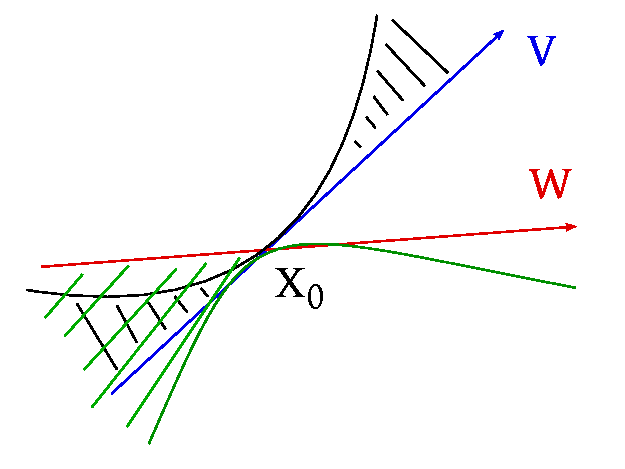
\includegraphics{img/36_dir.pdf}
          \caption{$v$ and $w$}
          \label{img:vandw}
        \end{center}
      \end{figure}

      Let $\varepsilon > 0$ be sufficiently small such that $\varphi(t) > \varphi(0) \forall \card{t} < \varepsilon, t \neq 0$.
      and $\psi(t) < \psi(0) \forall \card{t} < \varepsilon$ with $t \neq 0$.
      Then $f(x_0 + tv) = \varphi(t) > \varphi(0) = f(x_0)$ and $x_0 + tv = x$
      \[ \text{and } \norm{x - x_0} = \norm{tv} = \card{t} \cdot \norm{v} = \card{t} \cdot 1 < \varepsilon \]
      \[ \text{and } f(\underbrace{x_0 + tw}_{y}) = \psi(t) < \psi(0) = f(x_0) \]
      \[ \norm{y - x_0} = \norm{tw} = \card{t} \norm{w} = \card{t} \cdot 1 < \varepsilon \]
      Thus, $x_0$ is not a local extreme value.
      Compare with Figure~\ref{img:vandw}.
  \end{enumerate}
\end{proof}

\begin{remark}[Sufficient optimality conditions for the scalar case]
  \[ f''(x_0) > 0 \lor f''(x_0) < 0 \]
  \[ f''(x_0) = 0 \implies \text{ no conclusion} \]
  $f''(x_0) = 0$ gives a saddle point.

  In the 2-dimensional case, we have
  \[ D_2 f(x_0) \text{ symmetrical, positive definite} \]
  \[ Df(x_0) = 0 \]
  Compare with Figure~\ref{img:sad}~(a).

  \[ D_2 f(x_0) \text{ indefinite} \]
  \[ D f(x_0) = 0 \]
  $\rightarrow$ no extreme value. Compare with Figure~\ref{img:sad}~(b).

  \begin{figure}[t]
    \begin{center}
      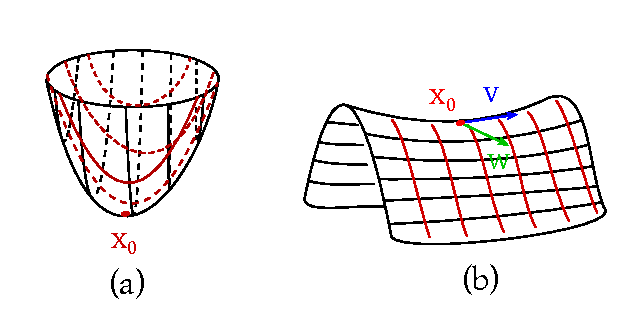
\includegraphics{img/36b_objects.pdf}
      \caption{(a) local minimum and (b) saddle point}
      \label{img:sad}
    \end{center}
  \end{figure}
\end{remark}

\section{Differential geometry of curves}

We consider:
\begin{enumerate}
  \item Maps $\gamma: I \subseteq \mathbb R \to \mathbb R^n$ (Figure~\ref{img:maps-diffgeo})
    \begin{figure}[t]
      \begin{center}
        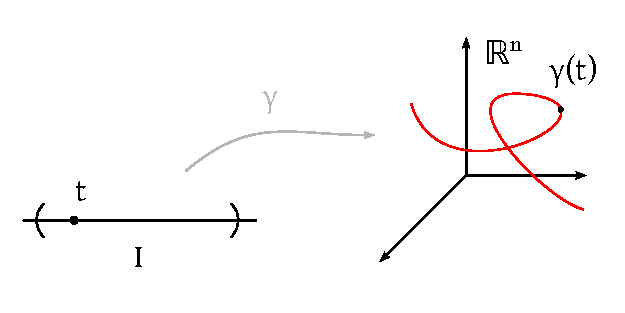
\includegraphics{img/37_map.pdf}
        \caption{Maps in differential geometry}
        \label{img:maps-diffgeo}
      \end{center}
    \end{figure}
  \item geometric properties of $\Gamma = \gamma(I)$.
\end{enumerate}

\index{Parameterized curve}
\index{Curvature}
\index{Regular curve parameterization}
\begin{definition} % Definition 1
  Let $I \subseteq \mathbb R$ be an interval.
  Let $\gamma: I \to \mathbb R^n$ be a continuous (or differentiable or smooth) function.
  Then $\gamma$ is a continuous (or differentiable or smooth) function curve parameterization.
  Colloquially, we are used to call $\gamma$ a \emph{parameterized curve} (in German: \foreignlanguage{german}{$\gamma$ is eine parametrisierte Kurve}).

  $\gamma(t) \in \mathbb R^n$ is a curve point.
  $t$ is the curve parameter.
  \[ \Gamma = \gamma(I) = \set{\gamma(t): t \in I} \subseteq \mathbb R^n \]
  is called trace of the curve parameterization.
  \[ \gamma(t) = \begin{bmatrix} \gamma_1(t) \\ \gamma_2(t) \\ \vdots \\ \gamma_n(t) \end{bmatrix} \]
  If $\gamma$ is differentiable, then
  \[ D\gamma(t)
        = \begin{bmatrix} \partial_t \gamma_1(t) \\ \partial_t \gamma_2(t) \\ \vdots \\ \partial_t \gamma_m(t) \end{bmatrix}
        = \begin{bmatrix} \gamma'_1(t) \\ \gamma'_2(t) \\ \vdots \\ \gamma'_n(t) \end{bmatrix} \eqqcolon \gamma'(t)
  \]
  $\gamma'(t)$ is the derivative vector. Often we also use the notation $\dot{\gamma}(t)$.

  Let $\gamma: I \to \mathbb R^n$ be differentiable.
  $\gamma$ is called \emph{regular curve parameterization} if $\gamma'(t) \neq 0 \forall t \in I$.
\end{definition}

\index{Unit tangential vector}
\index{Tangent of a curve}
\begin{definition} % Definition 2
  Let $\gamma: I \to \mathbb R^n$ be a regular curve parameterization.
  Let $T_\gamma(t) = \frac{\gamma'(t)}{\norm{\gamma'(t)}_2}$.
  $T_\gamma(t)$ is called \emph{unit tangential vector} of $\gamma$ in point $x = \gamma(t)$.
  \[ \tau(\gamma, x) = \set{x + \tau \cdot T_{\gamma}(t): \tau \in \mathbb R} \]
  is a line in $\mathbb R^n$ with directional vector $T_\gamma(t)$ through $x = \gamma(t)$.
  $\tau(\gamma, x)$ is called \emph{tangent} on $\Gamma$ in point $x$.
  Compare with Figure~\ref{img:tangent}.

  \begin{figure}[t]
    \begin{center}
      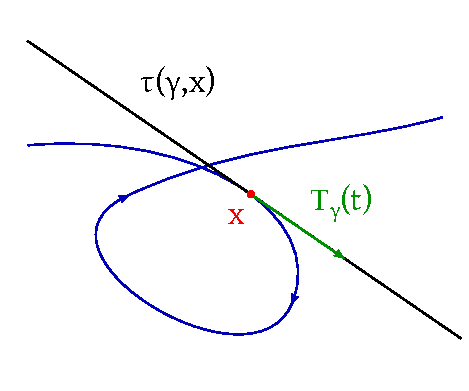
\includegraphics{img/38_tangent.pdf}
      \caption{$\tau(\gamma, x)$ is called \emph{tangent} on $\Gamma$ in point $x$}
      \label{img:tangent}
    \end{center}
  \end{figure}

  Motivation:
  \begin{align*}
    \gamma(t + \tau) &= \gamma(t) + \gamma'(t) \cdot \tau + o(\tau) \\
      &= \underbrace{x + \frac{\tau}{\norm{\gamma'(t)}} \cdot T_{\gamma}(t)}_{\in \tau(\gamma, x)} + o(\tau)
  \end{align*}
  A tangent is the best linear approximation of the curve.
\end{definition}

\dateref{2018/06/19}

\index{Reparameterization}
\begin{definition} % Definition 3
  Let $\gamma: I \to \mathbb R^n$ be a continuous or differentiable or smooth curve parameterization.
  Furthermore let $\sigma: J \to I$ with $J \subseteq \mathbb R$ as interval.

  Let $\sigma$ be a
  \begin{itemize}
    \item homeomorphim (continuous curve)
    \item diffeomorphism (differentiable curve)
    \item $\mathcal C^\infty$-diffeomorphism (smooth curve)
  \end{itemize}
  Then we call $\tilde \gamma: J \to \mathbb R^n$ with $\tilde \gamma = \gamma \circ \sigma$ a \emph{reparameterization} of $\gamma$.
  Compare with Figure~\ref{img:reparam}.

  \begin{figure}[t]
    \begin{center}
      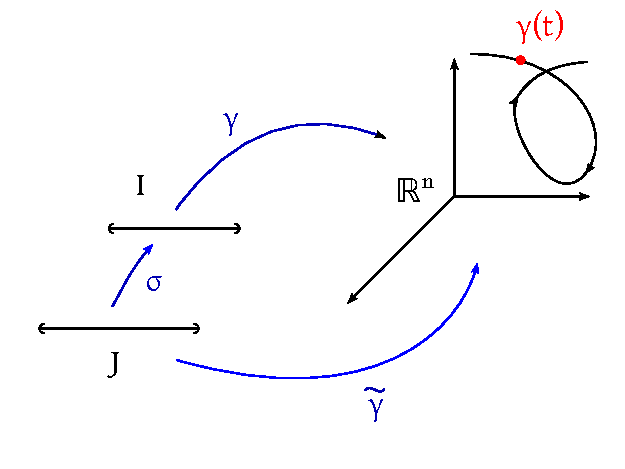
\includegraphics{img/40_reparameterization.pdf}
      \caption{Reparameterization}
      \label{img:reparam}
    \end{center}
  \end{figure}

  On the opposite, let $\gamma$, $\tilde \gamma$ be a curve parameterization. Then $\tilde\gamma$ is called reparameterization of $\gamma$ if $\sigma$ exists as above such that $\tilde \gamma = \gamma \circ \sigma$.
\end{definition}

\index{Homeomorphism}
\index{$\mathcal C^{\infty}$-Homeomorphism}
\begin{definition}[Discussion of terminology]
  Let $X, Y$ be topological spaces. $f: X \to Y$ is called \emph{homeomorphism}
  if $f$ is continuous and bijective and furthermore $f^{-1}: Y \to X$ is also continuous.

  Equivalently, for $\mathcal C^\infty$-diffeomorphism, $f$ is smooth and $f^{-1}$ is smooth.
\end{definition}

$\sigma: J \to I$ is bijective and continuous, hence $\sigma$ is either strictly monotonically increasing or strictly monotonically decreasing.

\begin{figure}[t]
  \begin{center}
    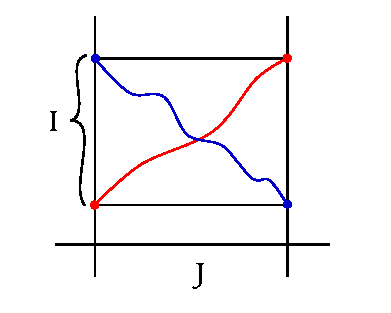
\includegraphics{img/41_orientation_preserving.pdf}
    \caption{Orientation}
    \label{img:orient}
  \end{center}
\end{figure}

\index{Orientation preserving reparameterization}
\index{Orientation reversing reparameterization}
\index{Parameter exchange}
\begin{definition}
  If $\sigma$ is strictly monotonically increasing, we call a reparameterization \emph{orientation preserving}.
  If $\sigma$ is strictly monotonically decreasing, we call a reparameterization \emph{orientation reversing}.
  Compare with Figure~\ref{img:orient}.

  ($\sigma$ is a diffeomorphism, $\sigma' > 0$ and accordingly $\sigma' < 0$ defines the orientation. $\sigma$ is called \emph{parameter exchange})
\end{definition}

\begin{claim}
  Let $G = \set{\gamma: \gamma \text{ is a regular curve parameterization}}$.
  We define a relation $\sim_{r}$ on $G$. $\gamma \sim_r \tilde\gamma \iff \tilde\gamma$ is a reparameterization of $\gamma$.
  Then $\sim_r$ is an equivalence relation.
\end{claim}
\begin{proof}
  \begin{description}
    \item[Reflexivity]
      $\gamma \sim_r \gamma$ with $\sigma: I \to I$, $\sigma = \operatorname{id}$. 
    \item[Symmetry]
      Let $\tilde\gamma \sim_r \gamma$, hence $\tilde\gamma = \gamma \circ \sigma \implies \tilde\gamma \circ \sigma^{-1} = \gamma \implies \gamma \sim_r \tilde\gamma$.
    \item[Transitivity]
      Let $\tilde{\tilde\gamma} \sim_r \tilde\gamma$ and $\tilde\gamma \sim_r \gamma$, hence $\tilde{\tilde\gamma} = \tilde\gamma \circ \rho$.
      $\tilde\gamma = \gamma \circ \sigma \implies \tilde{\tilde\gamma} = \gamma \circ \sigma \circ \rho \implies \tilde{\tilde\gamma} \sim_r \gamma$ with $\sigma \circ \rho$ as diffeomorphism.
  \end{description}
\end{proof}

\index{Geometrical quantity}
\begin{definition}
  Let $[\gamma]_{\sim_r}$ be an equivalence class of $\gamma$ in regards of $\sim_r$. A size or property, which only depends on $[\gamma]_{\sim_n}$ but not on a specific representative $\gamma$ is called \emph{geometrical quantity}.
\end{definition}

\index{Closed curve}
\begin{example}
  $[\gamma]_{\sim_r}$ is called \emph{closed curve} if $\gamma(a) = \gamma(b)$ with $\gamma: [a,b] \to \mathbb R^n$.
  Later, we will show: arc length is a geometrical property.

  Because $\gamma(t) = \tilde{\gamma}(\sigma(\tau))$ with $\tau = \sigma^{-1}(t)$, parameterizations have the same trace $\Gamma = \gamma(I) = \tilde\gamma(J)$. Sometimes we call $[\gamma]_{\sim_r}$ a curve in $\mathbb R^n$.
\end{example}

\begin{example}
  \label{exx}
  Let $I = [0,2\pi]$. $\gamma(t) \coloneqq \begin{bmatrix} \cos(t) \\ \sin(t) \end{bmatrix}$. $\gamma: I \to \mathbb R^2$.
  It holds $\gamma(0) = \gamma(2\pi)$, hence $\gamma$ is closed. Compare with Figure~\ref{img:ex1}.

  \begin{figure}[t]
    \begin{center}
      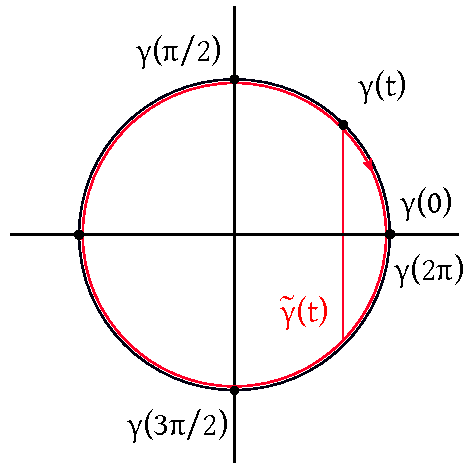
\includegraphics{img/52a_ex.pdf}
      \caption{Example~\ref{exx}}
      \label{img:ex1}
    \end{center}
  \end{figure}

  \[ \sigma: [-2\pi, 0] \to [0, 2\pi] \]
  \[ \sigma(t) = -t \]
  \[ \hat\gamma(t) = \begin{bmatrix} \cos(t) \\ -\sin(t) \end{bmatrix} \text{ with } t \in [0,2\pi] \]
  
  \begin{figure}[t]
    \begin{center}
      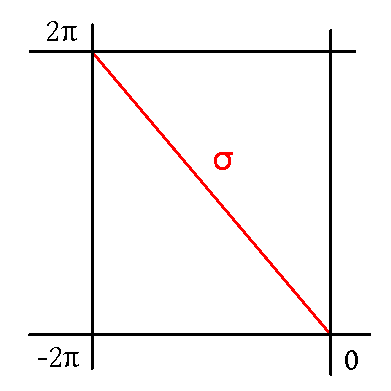
\includegraphics{img/52b_ex.pdf}
      \caption{Example~\ref{exx}}
      \label{img:ex1b}
    \end{center}
  \end{figure}

  \[ \gamma \circ \sigma(t) = \begin{bmatrix} \cos(-t) \\ \sin(-t) \end{bmatrix} = \begin{bmatrix} \cos(t) \\ -\sin(t) \end{bmatrix} = \tilde\gamma(t) \]
  with $\tilde\gamma(t): [-2\pi, 0] \to \mathbb R^2$ is periodical with period $2\pi$.
  Hence, $\tilde\gamma(t - 2\pi) = \tilde\gamma(t) \forall t \in \mathbb R$.
  \[ \hat\gamma(t) \coloneqq \tilde\gamma(t - 2\pi) \qquad \hat\gamma: [0, 2\pi] \]
  \[ \hat{\gamma}(t) = \begin{bmatrix} \cos(t) \\ -\sin(t) \end{bmatrix} \qquad \hat{\gamma}(t) = \gamma(\underbrace{-t + 2\pi}_{\sigma(t)}) \]
  with $\sigma'(t) = -1$. Hence reparameterization is orientation reversing.
\end{example}

\begin{example}
  \label{ex:ex}
  Let $\gamma: \mathbb R \to \mathbb R^2$.
  \[ \gamma(t) = \begin{bmatrix} t^2 - 1 \\ t^3 - t \end{bmatrix} \qquad \gamma'(t) = \begin{bmatrix} 2t \\ 3t^2 - 1 \end{bmatrix} \]
  \[ \gamma'(t) = 0 \implies 2t = 0 \text{ hence } t = 0 \]
  \begin{figure}[t]
    \begin{center}
      \includegraphics{img/53a_example.pdf}
      \caption{Example~\ref{ex:ex}}
      \label{img:examp}
    \end{center}
  \end{figure}
  Compare with Figure~\ref{img:examp}.
  Then $3t^2 - 1 = -1 \neq 0$ follows.
  So the parameterization is \emph{regular}. It holds that $\gamma(1) = \vectwo 00$ and $\gamma(-1) = \vectwo 00$.
  $\vectwo 00$ lies on the trace of the curve for 2 different parameter values.
  $x = 0$ is a double point of the curve.
  \[ \gamma'(-1) = \begin{bmatrix} -2 \\ 2 \end{bmatrix} \qquad T_{\gamma}(-1) = \frac1{\sqrt{2}} \begin{bmatrix} -1 \\ 1 \end{bmatrix} \]
  \[ \gamma'(1) = \begin{bmatrix} 2 \\ 2 \end{bmatrix} \qquad T_{\gamma}(1) = \frac1{\sqrt{2}} \begin{bmatrix} 1 \\ 1 \end{bmatrix} \]
  For parameter values $t = -1$ and $t = 1$, tangents exist. But in $x = 0 = \gamma(1) = \gamma(-1)$, no tangent exists.
\end{example}

\begin{example}
  \label{ex:e}
  Let $\gamma: \mathbb R \to \mathbb R^2$.
  \[ \gamma(t) = \begin{bmatrix} t^2 \\ t^3 \end{bmatrix} \qquad \text{\enquote{Neil's parabola}} \]
  \[ \gamma(0) = \begin{bmatrix} 0 \\ 0 \end{bmatrix} \qquad \gamma'(t) = \begin{bmatrix} 2t \\ 3t^2 \end{bmatrix} \qquad \gamma'(t) = \begin{bmatrix} 0 \\ 0 \end{bmatrix} \]
  \begin{figure}[t]
    \begin{center}
      \includegraphics{img/53b_example.pdf}
      \caption{Example~\ref{ex:e}}
      \label{img:example}
    \end{center}
  \end{figure}
  Compare with Figure~\ref{img:example}.
  Curvature parameterization is not regular.
  For $t = 0$, no tangent exists.
\end{example}

\begin{example}
  \[ \gamma(t) = \begin{bmatrix} t^3 \\ t^3 \end{bmatrix} \qquad \gamma'(t) = \begin{bmatrix} 3t^2 \\ 3t^2 \end{bmatrix} \]
  with $\gamma'(0) = \begin{bmatrix} 0 \\ 0 \end{bmatrix}$ is non-regular.
  \begin{figure}[t]
    \begin{center}
      \includegraphics{img/54a_gamma.pdf}
      \caption{$\Gamma: \gamma(\mathbb R)$}
      \label{img:Gamma}
    \end{center}
  \end{figure}
  Compare with Figure~\ref{img:Gamma}.
  $\Gamma$ is smooth has a \enquote{geometrical} tangent everywhere.
\end{example}

Let $\sigma$ be an orientation preservering parameter exchange.
\[ \tilde\sigma = \gamma \circ \sigma \qquad \gamma(t) = \tilde\gamma(\tau) \]
with $t = \sigma(\tau)$ and $\tau = \sigma^{-1}(t)$. Let $\gamma$ be regular.

\[ T_{\gamma}(t) = \frac{\gamma'(t)}{\norm{\gamma'(t)}} \]
\[ \tilde\gamma'(t) = (\gamma \circ \sigma)'(\tau) = \gamma'(\sigma(\tau)) \cdot (\sigma)'(\tau) = \gamma'(t) \cdot \underbrace{\sigma'(\tau)}_{> 0} \]
\[ \implies \norm{\tilde\gamma'(\tau)}_2 = \norm{\gamma'(t) \cdot \sigma'(\tau)}_2 = \sigma'(\tau) \norm{\gamma'(t)}_2 \]
\[ T_{\tilde\gamma}(\tau) = \frac{\tilde\gamma'(\tau)}{\norm{\gamma'(\tau)}_2} = \frac{\gamma'(t) \cdot \sigma'(\tau)}{\norm{\gamma'(t)} \sigma'(\tau)} = T_{\gamma}(t) \]
Let $\sigma$ be orientation reversing.
\[ \gamma'(\tau) < 0 \qquad \card{\gamma'(\tau)} = -\sigma'(\tau) \]
like above $\tilde\sigma'(\tau) = \gamma'(t) \cdot \sigma'(\tau)$ and $\norm{\tilde\gamma'(\tau)}_2 = \card{\sigma'(\tau)} \cdot \norm{\gamma'(t)}_2 = -\sigma'(\tau) \norm{\gamma'(t)}_2$.
\[ T_{\tilde\gamma}(\tau) = -T_{\gamma}(t) \]
Compare with Figure~\ref{img:ori}.

\begin{figure}[t]
  \begin{center}
    \includegraphics{img/45b_orientation.pdf}
    \caption{$T_{\tilde\gamma}(\tau) = -T_{\gamma}(t)$}
    \label{img:ori}
  \end{center}
\end{figure}

\subsection{Arc length of parameterized curves}
\index{Rectifiable curve}
\index{Arc length of a curve}
\begin{definition} % Definition 4
  Let $I = [a,b]$ be compact. $\gamma: I \to \mathbb R^n$ is a continuous curve.
  \[ Z = (t_0 = a < t_1 < t_2 < \dots < t_N = b) \]
  a partition of interval $[a,b]$. Let 
  \[ S_\gamma(z) = \sum_{k=1}^N \norm{\gamma(t_k) - \gamma(t_{k-1})}_2 \]
  be the length of the polygonial line through points $(x_k)_{k=0}^N$ with $x_k = \gamma(t_k)$.

  \pic{img/46_polygonial_line.pdf}{Polygonial line}

  If $S_{\gamma} < \infty$, then $\gamma$ is called \emph{rectifiable}
  and $S_{\gamma}$ is the \emph{arc length of the curve}.
\end{definition}

\begin{remark}
  Let $\tilde\gamma$ be a reparameterization of $\gamma$.
  Let $t = \sigma(\tau)$ be a parameter exchange and $\sigma: [\alpha, \beta] \to [a,b]$.
  $t_k = \sigma(\tau_k)$ with $k = 0, \dots, N$.
  If $\sigma$ is orientation preservering, then $\tilde Z = \set{\tau_0 = \alpha < \tau_1 < \dots < \tau_N = \beta}$ is a partition of $[\alpha, \beta]$.
  If $\sigma$ is orientation reversing, then $\tilde Z = \set{\alpha = \tau_N < \tau_{N-1} < \dots < \tau_0 = \beta}$ is a partition.
  In every case,
  \[ S_{\gamma}(Z) = S_{\tilde\gamma}(\tilde Z) \]
  because $x_k = \gamma(t_k) = \tilde\gamma(\tau_k)$ and accordingly $x_k = \gamma(t_k) = \tilde\gamma(\tau_{N-k})$.
  So $S_\gamma$ is a geometrical quantity.
\end{remark}

\begin{lemma} % Lemma 1
  Let $\gamma: [a, b] \to \mathbb R^n$ be Lipschitz continuous, hence $\exists L \geq 0$ such that $\norm{\gamma(s) - \gamma(t)}_2 \leq L \card{s - t} \forall s, t \in [a,b]$. Then $\gamma$ is rectifiable.
\end{lemma}

\begin{proof}
  Let $Z$ be a partition of $[a,b]$. $Z = (t_k)_{k=0}^N$. Then
  \[ S_{\gamma}(Z) = \sum_{k=1}^N \norm{\gamma(t_k) - \gamma(t_{k-1})}_2 \underbrace{\leq}_{\substack{\text{by Lipschitz} \\ \text{continuity}}} \sum_{k=1}^N L \underbrace{\card{t_k - t_{k-1}}}_{\substack{= t_k - t_{k-1} \\ \text{ because } t_k > t_{k-1}}} \]
  \[ = \sum_{k=1}^N L(t_k - t_{k-1}) = L(t_N - t_0) = L(b - a) < \infty \]
  hence $\sup\set{S_{\gamma}(z): z \text{ partition}} \leq L(b - a) < \infty$.
\end{proof}

\begin{lemma} % Lemma 2
  \label{lemma-2}
  Let $\alpha: [a,b] \to \mathbb R^n$. $\alpha(t) = \left[\alpha_1(t), \alpha_2(t), \dots, \alpha_n(t)\right]^T$.
  $\alpha_n \in \mathcal R[a,b]$ for $k = 1, \dots, n$.
  \[ \int_a^b \alpha(t) \, dt = \left[\int_a^b \alpha_1 \, dt, \int_a^b \alpha_2 \, dt, \dots, \int_a^b \alpha_n \, dt\right]^T \]
  \[ \text{Then } \norm{\int_a^b \alpha \, dt}_2 \leq \int_a^b \norm{\alpha(t)}_2 \, dt \]
\end{lemma}

\begin{proof}
  Approximation by step functions: Let $\varphi: [a,b] \to \mathbb R^n$.
  $\gamma(t) = \left[\varphi_1(t), \dots, \varphi_n(t)\right]^T$.
  $\gamma_i \in \tau[a,b]$. Without loss of generality all $\varphi_i$ are step functions in regards of the same partition $Z = (t_k)_{k=0}^N$\footnote{If not, take the union of two non-equal-sized intervals and apply the lemma to a refinement of this new interval again. Therefore without loss of generality.}.
  \[ \varphi_i(t) = C_i^k \text{ for } t \in (t_{k-1}, t_k) \]
  \[ \int_a^b \varphi_i \, dt = \sum_{k=1}^N c_i^k (t_k - t_{k-1}) \]
  $\varphi_i$ should approximate $\alpha_i$ uniformly, hence for $\varepsilon > 0$ arbitrarily chosen, choose $\varphi_i$ such that
  \[ \card{\varphi_i(t) - \alpha_i(t)} < \frac{\varepsilon}{2 \sqrt n (b - a)} \qquad \forall t \in [a,b] \]
  For step function $\varphi$,
  \[ \norm{\int_a^b \varphi \, dt}_2 = \norm{\sum_{k=1}^N (t_k - t_{k-1}) \left[c_1^k, c_2^k, \dots, c_n^k\right]^T} \]
  By the triangle inequality in $\mathbb R^n$,
  \[ \leq \sum_{k=1}^n (t_k - t_{k-1}) \cdot \underbrace{\norm{\left[c_1^k, \dots, c_n^k\right]^T}_2}_{\norm{\varphi(t)}_2 \text{ for } t \in (t_{k-1}, t_k)} = \int_a^b \norm{\varphi} \, dt \]
\end{proof}

\dateref{2018/06/21}

\begin{proof}[continued]
  Let $\alpha$ as in the lemma statement.
  Let $\varepsilon > 0$ be arbitrary and $\varphi_k \in \tau[a,b]$ such that $\card{\alpha_k(t) - \varphi_k(t)} < \frac{\varepsilon}{2 \sqrt{n} (b - a)} \forall t \in [a,b] \forall k = 1, \dots, n$. Hence,
  \begin{align*}
    \int_a^b \norm{\alpha - \varphi}_2 \, dt &= \int_a^b \sqrt{\sum_{k=1}^n \card{\alpha_k(t) - \varphi_k(t)}^2 \, dt}     & \varphi \coloneqq [\varphi_1, \dots, \varphi_n]^n \\
        &\leq \int_a^b \sqrt{\underbrace{\sum_{k=1}^n \frac{\varepsilon^2}{4n (b - a)^2}}_{= \frac{\varepsilon^2}{4 (b - a)^2}}} \, dt
        = \int_a^b \frac{\varepsilon}{2 (b - a)} \, dt
  \end{align*}
  \[ (b - a) \cdot \frac{\varepsilon}{2 (b - a)} = \frac{\varepsilon}{2} \]
  Also,
  \begin{align*}
    \norm{\int_a^b (\alpha - \varphi) \, dt}_2
      &= \norm{\begin{bmatrix} \int_a^b (\alpha_1 - \varphi_1) \, dt \\ \vdots \\ \int_a^b (\alpha_n - \varphi_n) \, dt \end{bmatrix}}_2
      = \norm{\begin{bmatrix} \card{\int_a^b (\alpha_1 - \varphi_1) \, dt} \\ \vdots \\ \card{\int_a^b (\alpha_n - \varphi_n)} \, dt \end{bmatrix}}_2 \\
      &= \norm{\begin{bmatrix} \int_a^b \card{\alpha_1 - \varphi_1} \, dt \\ \vdots \\ \int_a^b \card{\alpha_n - \varphi_n} \, dt \end{bmatrix}}_2
      \leq \norm{\begin{bmatrix} \int_a^b \frac{\varepsilon}{2\sqrt n (b - a)} \, dt \\ \vdots \\ \int_a^b \frac{\varepsilon}{2 \sqrt n (b - a)} \end{bmatrix}}_2
      = \norm{\begin{bmatrix} \frac{\varepsilon}{2 \sqrt n} \\ \vdots \\ \frac{\varepsilon}{2 \sqrt n} \end{bmatrix}}_2 \\
      &= \sqrt{\sum_{k=1}^n \frac{\varepsilon^2}{4n}} = \frac\varepsilon2
  \end{align*}
  Hence, $\norm{\int_a^b \alpha \, dt} = \norm{\int_a^b (\alpha - \varphi) \, dt + \int_a^b \varphi \, dt}_2 \leq \norm{\int_a^b (\alpha - \varphi) \, dt}_2 + \norm{\int_a^b \varphi \, dt} \leq \frac{\varepsilon}{2} + \int_a^b \norm{\varphi}_2 \, dt$ because $\varphi \in \tau[a,b]$.
  \begin{align*}
      &\leq \frac{\varepsilon}{2} + \int_a^b \norm{\varphi - \alpha + \alpha}_2 \, dt \\
      &\leq \frac{\varepsilon}{2} + \underbrace{\int_a^b \norm{\varphi - \alpha}_2 \, dt}_{\leq \frac\varepsilon2} + \int_a^b \norm{\alpha}_2 \, dt \\
      &\leq \varepsilon + \int_a^b \norm{\alpha}_2 \, dt \\
    \implies \: & \norm{\int_a^b \alpha \, dt}_2 \leq \varepsilon + \int_a^b \norm{\alpha}_2 \, dt \forall \varepsilon > 0 \\
    \implies \: & \norm{\int_a^b \alpha \, dt}_2 \leq \int_a^b \norm{\alpha} \, dt
  \end{align*}
\end{proof}

\begin{theorem} % Satz 1
  Let $\gamma: [a,b] \to \mathbb R^n$ be a continuous curve parameterization.
  $\gamma(t) = [\gamma_1(t), \dots, \gamma_n(t)]^T$ and let $\gamma_k$ be a antiderivative of regulated function $\alpha_k = \gamma'_k(t)$.
  Then $\gamma$ is rectifiable and:
  \[ S_\gamma = \int_a^b \norm{\gamma'(t)}_2 \, dt \]
\end{theorem}

\begin{proof}
  Let $z = (t_i)_{i=0}^N$ be a partition of $[a,b]$.
  \begin{align*}
    S_\gamma(z)
      &= \sum_{i=1}^N \norm{\gamma(t_i) - \gamma(t_{i-1})}_2 \\
      &\underbrace{=}_{\substack{\text{fundamental} \\ \text{theorem}}} \sum_{i=1}^N \norm{\int_{t_{i-1}}^{t_i} \gamma'(t) \, dt}_2 \\
      &\underbrace{\leq}_{\text{Lemma~\ref{lemma-2}}} \sum_{i=1}^N \int_{t_{i-1}}^{t_i} \norm{\gamma'(t)}_2 \, dt \\
      &= \int_{t_0}^{t_N} \norm{\gamma'(t)}_2 \, dt \\
      &= \int_a^b \norm{\gamma'(t)}_2 \, dt
  \end{align*}
  So, $S_{\gamma}(z) \leq \int_a^b \norm{\gamma'(t)}_2 \, dt \forall z$ partitions.
  Therefore, $S_{\gamma} \leq \int_a^b \norm{\gamma'(t)}_2 \, dt$ and $\gamma$ is rectifiable.

  Show: $\forall \varepsilon > 0$, $S_\gamma \geq \int_a^b \norm{\gamma'(t)}_2 \, dt - \varepsilon$. $\gamma'$ is a regulated function. Choose $\varphi = [\varphi_1, \dots, \varphi_n]^T$ with $\varphi_k \in \tau[a,b]$ with $\norm{\varphi(t) - \gamma'(t)} \leq \frac{\varepsilon}{2(b - a)} \forall t \in [a,b]$.
  \[ \varphi(t) = \begin{bmatrix} c_i^1 \\ c_i^2 \\ \vdots \\ c_i^n \end{bmatrix} \text{ on } (t_{i-1}, t_i) \]
  \[ \implies \norm{\int_{t_{i-1}}^{t_i} \varphi \, dt}_2 = \norm{\begin{bmatrix} c_i^1 \\ \vdots \\ c_n^i \end{bmatrix} \cdot (t_i - t_{i-1})}_2 = (t_i - t_{i_1}) \norm{\begin{bmatrix} c_i^1 \\ \vdots \\ c_i^n \end{bmatrix}}_2 \]
  \[ \int_{t_{i-1}}^{t_i} \norm{\varphi} \, dt = \int_{t_{i-1}}^{t_i} \norm{\begin{bmatrix} c_i^1 \\ \vdots \\ c_i^n \end{bmatrix}}_2 \, dt = (t_i - t_{i-1}) \norm{\begin{bmatrix} c_i^1 \\ \vdots \\ c_i^n \end{bmatrix}}_2 \]
  Hence, for $(t_{i-1}, t_i)$
  \[ \int_{t_{i-1}}^{t_i} \norm{\varphi} \, dt = \norm{\int_{t_{i-1}}^{t_i} \varphi \, dt} \]
%  \[ \int_a^b \norm{\gamma'(t)}_2 \, dt = \int_a^b \norm{\varphi - (\varphi - \gamma')}_2 \, dt \]
%  \[ \geq \int_a^b \norm{\varphi}_2 \, dt = \int_a^b \norm{\varphi - \gamma'}_2 \, dt \]
%  \[ \geq \sum_{i=1}^N \int_{t_{i-1}}^{t_i} \norm{\varphi}_2 \, dt - \int_a^b \frac{\varepsilon}{2 (b - a)} \, dt = \sum_{i=1}^N \norm{\int_{t_{i-1}}^{t_i} \varphi} \]
  \[ \norm{\gamma(t_i) - \gamma(t_{i-1})}_2 = \norm{\int_{t_{i-1}}^{t_i} \gamma'(t) \, dt}_2 \]
  \[ = \norm{\int_{t_{i-1}}^{t_i} \left[\varphi(t) - (\varphi(t) - \gamma'(t))\right] \, dt}_2
       \geq \norm{\int_{t_{i-1}}^{t_i} \varphi(t) \, dt}_2 - \norm{\int_{t_{i-1}}^{t_i} (\varphi - \gamma') \, dt}_2 \]
  Because $\norm{\int_{t_{i-1}}^{t_i} \varphi(t) \, dt}_2 = \int_{t_{i-1}}^{t_n} \norm{\gamma}_2 \, dt$,
  \[ \geq \int_{t_{i-1}}^{t_i} \norm{\varphi}_2 \, dt - \int_{t_{i-1}}^{t_i} \underbrace{\norm{\varphi - \gamma'}_2}_{\leq \frac{\varepsilon}{2 (b - a)}} \, dt \]
  \[ \geq \int_{t_{i-1}}^{t_i} \norm{\varphi}_2 \, dt - \frac{\varepsilon (t_i - t_{i-1})}{2 (b - a)} \]
  \begin{align*}
    S_\gamma(z) &= \sum_{i=1}^N \norm{\int_{t_{i-1}}^{t_i} \gamma'(t) \, dt} \\
                &\geq \sum_{i=1}^n \int_{t_{i-1}}^{t_i} \norm{\varphi}_2 \, dt - \frac{\varepsilon}{2(b - a)} (t_i - t_{i-1}) \\
                &= \int_a^b \norm{\varphi}_2 \, dt - \frac{\varepsilon}{2} \\
                &= \int_a^b \norm{\gamma' - (\gamma' - \varphi)}_2 \, dt - \frac\varepsilon2 \\
                &\geq \int_a^b \norm{\gamma'} \, dt - \int_a^b \norm{\underbrace{\gamma' - \varphi}_{\leq \frac\varepsilon{2 (b - a)}}}_2 \, dt - \frac\varepsilon2 \\
                &\geq \int_a^b \norm{\gamma'(t)}_2 \, dt - \frac\varepsilon{2(b - a)} \cdot (b - a) - \frac\varepsilon2 \\
                &= \int_a^b \norm{\gamma'(t)}_2 \, dt - \varepsilon
  \end{align*}
  \[ \implies S_\gamma \geq S_\gamma(z) \geq \int_a^b \norm{\gamma'(t)}_2  \, dt - \varepsilon \qquad \forall \varepsilon > 0 \]
  \[ \implies S_\gamma \geq \int_a^b \norm{\gamma'(t)}_2 \, dt \]
\end{proof}

\begin{remark}
  By definition of $S_\gamma$, the arc length is a geometrical quantity.
\end{remark}

\begin{remark}
  Another rationale for the independence of parameterization:

  Let $\gamma: I \to \mathbb R^n$ be a regular $\mathcal C^1$-curve parameterization.
  Let $\sigma: J \to I$ be a parameter exchange (diffeomorphism).
  $\tilde\gamma(\tau) = \gamma \circ \sigma(\tau)$.

  $\sigma$ is orientation preserving. $J = [\alpha, \beta], I = [a,b] \implies \sigma(\alpha) = a, \sigma(\beta) = b$.
  \[ S_{\tilde\gamma} = \int_\alpha^\beta \norm{\tilde\gamma'(\tau)}_2 \, d\tau = \int_\alpha^\beta \norm{[\gamma(\sigma(\tau))]'}_2 \, d\tau = \int_\alpha^\beta \norm{\gamma'(\sigma(\tau)) \cdot \underbrace{\sigma'(\tau)}_{> 0}}_2 \, d\tau \]
  \[ = \int_\alpha^\beta \norm{\gamma'(\sigma(\tau))} \cdot \sigma'(\tau) \, d\tau \overbrace{=}^{\substack{\text{transformation} \\ \text{theorem}}} \int_a^b \norm{\gamma'(t)}_2 \, dt = S_\gamma \]
  Let $\sigma$ be orientation reversing, hence $\sigma'(\tau) < 0$. $\sigma(\alpha) = b$ and $\sigma(\beta) = a$.
  \[ S_{\tilde\gamma} = \int_{\alpha}^\beta \norm{\tilde\gamma'(\tau)}_2 \, d\tau = \int_{\alpha}^{\beta} \norm{\gamma'(\sigma(\tau)) \cdot \underbrace{\sigma'(\tau)}_{< 0}}_2 \, d\tau = -\int_{\alpha}^{\beta} \norm{\gamma'(\sigma(\tau))}_2 \underbrace{\sigma'(\tau)}_{= -\card{\sigma'(\tau)}} \, dt \]
  \[ = \int_\beta^\alpha \norm{\gamma'(\sigma(\tau))}_2 \cdot \sigma'(\tau) \, d\tau = \int_{\sigma(\beta)}^{\sigma(\alpha)} \norm{\gamma'(t)}_2 \, dt = \int_a^b \norm{\gamma'(t)}_2 \, dt \]
\end{remark}

Idea: Define $s = l(t) = \int_{t_0}^t \norm{\gamma'(\tau)}_2 \, d\tau$. Compare with Figure~\ref{img:traversedpath}.

\begin{figure}[t]
  \begin{center}
    \includegraphics{img/47_traversed_path.pdf}
    \caption{Traversed path}
    \label{img:traversedpath}
  \end{center}
\end{figure}

For $\tilde t < t$, $l(\tilde t) = \int_{t}^{\tilde t} \norm{\gamma'(\tau)}_2 \, d\tau = -\underbrace{\int_{\tilde t}^{t} \norm{\gamma'(\tau)}_2 \, d\tau}_{> 0} < 0$.

\index{Arc length parameter}
\begin{definition}
  We call $s = l(t) = \int_{t_0}^t \norm{\gamma'(\tau)}_2 \, d\tau$ the arc length parameter of the curve parameterization $\gamma$.
\end{definition}

Let $\gamma$ be regular. Then (by the Fundamental Theorem) $l$ is continuously differentiable and
\[ l'(t) = \frac{d}{dt} \left[\int_{t_0}^t \norm{\gamma'(\tau)}_2 \, d\tau\right] = \norm{\gamma'(t)}_2 > 0 \]
Hence, $l$ is strictly monotonically increasing.

Let $I = [a,b]$. $t_0 \in I$ and $I$ is compact. Then $l: I \to J = l(J)$ is strictly monotonically increasing and continously differentiable. $J = [\alpha, \beta] = [l(a), l(b)]$. $l^{-1}: J \to I$ is also continuous. $l^{-1}$ is also continuously differentiable with
\[ (l^{-1})'(s) = \frac{1}{l'(l^{-1}(s))} = \frac{1}{\norm{\gamma'(t)}_2} > 0 \]
with $t = l^{-1}(s)$ and accordingly $s = l(t)$. $l^{-1}$ is strictly monotonically increasing and continously differentiable.

Let $\tilde\gamma(s) = \gamma \circ l^{-1}(s)$. Let $\tilde\gamma$ be the reparameterization of $\gamma$ by the arc length. Often we write $\gamma(s)$ instead of $\tilde\gamma(s)$. $s$ is a very common variable denoting the arc length parameter.
Often: $s = s(t)$ instead of $s = l(t)$, $t = s^{-1}(s)$ is inappropriate.

Let $\tilde\gamma$ be the reparameterization of $\gamma$ by the arc length. Then
\begin{align*}
  \tilde\gamma'(s) &= \frac d{ds} [\gamma(l^{-1}(s))]
    = \gamma' (l^{-1}(s)) (l^{-1})'(s)
    = \gamma' (t) \cdot \frac{1}{l'(t)}
    = \gamma' (t) \cdot \frac{1}{\norm{\gamma'(t)}_2} = T_{\gamma}(t)
\end{align*}
because for derivatives of inverse functions, $(f^{-1})'(x) = \frac{1}{f'(f^{-1}(x))}$.
So, $\norm{\tilde\gamma(s)}_2 = 1$. $\tilde\gamma'(s) = T_{\tilde\gamma}(s)$.

Determine the arc length for $\tilde\gamma$:
\[ \tilde l(s) = \int_0^s \underbrace{\norm{\tilde\gamma'(\xi)}_2}_{= 1} \, d\xi = s \]
\[ \tilde\gamma(0) = \gamma(t_0) \]

\begin{example}[Cycloid]
  \[ \gamma(t) = \begin{bmatrix} t - \sin(t) \\ 1 - \cos(t) \end{bmatrix} \]
  \begin{figure}
    \begin{center}
      \includegraphics{img/48_cycloid.pdf}
      \caption{Trace of a cycloid}
      \label{img:cycloid}
    \end{center}
  \end{figure}
  Figure~\ref{img:cycloid} illustrates the trace of a cycloid.
  \[ \gamma'(t) = \begin{bmatrix} 1 - \cos(t) \\ \sin(t) \end{bmatrix} \]
  \begin{align*}
    s &= \int_0^t \norm{\gamma'(\tau)}_2 \, d\tau = \int_0^t \sqrt{(1 - \cos\tau)^2 + \sin^2 \tau} \, d\tau \\
      &= \int_0^t \sqrt{1 - 2 \cos \tau + 1} \, d\tau = \int_0^t \sqrt2 \sqrt{1 - \cos2 \frac{\tau}{2}} \, d\tau \\
      &= \sqrt{2} \int_0^t \sqrt{\underbrace{1 - \cos^2{\frac\tau2}}_{= \sin^2{\frac\tau2}} + \sin^2{\frac\tau2}} \, d\tau \\
      &= \sqrt{2} \int_0^t \sqrt{2} \sqrt{\sin^2{\frac\tau2}} \, d\tau \\
    \intertext{
      $t \in [0, 2\pi] \implies \frac\tau2 \in [0, \pi] \implies \sin\frac\tau2 \geq 0$.
      $\sqrt{\sin^2(\frac\tau2)} = \sin(\frac\tau2)$
    }
      &= 2 \int_0^t \sin{\frac\tau2} \, d\tau = 2 \left[2 - \cos \frac{t}{2} + 2 \cos 0\right] \\
      &= 4 (1 - \cos\frac t2) = s \\
    l(t) &= 4 (1 - \cos\frac t2) \\
    l^{-1}(s) &= \text{ ?} \\
    1 - \cos\frac t2 &= \frac s4 \\
    \cos\frac t2 &= 1 - \frac s4 = \frac14 (4 - s) \in [-1, +1] \\
    t &= 2 \arccos\left(\frac14 (4 - s)\right) \\
    \tilde \gamma(s) &= \begin{bmatrix} 2 \arccos(\frac14 (4 - s)) - \sin(2 \arccos(\frac14 (4 - s))) \\ 1 - \cos(2 \arccos(\frac14(4 - s))) \end{bmatrix}
  \end{align*}
\end{example}

\begin{remark}
  The reparameterization by the arc length often do not yield algebraically simpler expression.
  But it provides the property, that the curve is traversed with uniform speed.
\end{remark}

\index{Parameterization by a curve's arc length}
\begin{definition} % Definition 5
  Let $\gamma: I \to \mathbb R^n$ be a regular curve.
  We call $\gamma$ \emph{parameterized by its arc length}, if $\norm{\gamma'(t)}_2 = 1 \forall t \in I$.
\end{definition}

\begin{remark}
  Let $\gamma$ be parameterized by an arc length.
  Then $s = l(t) = \int_{t_0}^t \underbrace{\norm{\gamma'(\tau)}_2}_{=1} \, d\tau = t - t_0$, and accordingly $t = s + t_0$.
  Hence, curve parameter and arc length parameter differ only by constant $t_0$. For $t_0 = 0$, $s = t$.
\end{remark}

Let $\gamma$ be regular and a $\mathcal C^2$ curve and $\norm{\gamma'(t)}_2 = 1 \forall t \in I$, hence $\gamma$ is parameterized by the arc length.

Consider $1 = \norm{\gamma'(t)}_2^2 = \left(\gamma'(t)\right)^T \cdot \gamma'(t)$. If we derive by $t$,
\[ 0 = \gamma''(t)^T \cdot \gamma'(t) + \gamma'(t)^T \cdot \gamma''(t) = 2 \angel{\gamma'(t), \gamma''(t)} \]
Hence $\gamma''(t)$ is orthogonal to $\gamma'(t)$. Compare with Figure~\ref{img:orthott}.

\begin{figure}[t]
  \begin{center}
    \includegraphics{img/49_orthogonal.pdf}
    \caption{Orthogonal $\gamma'(t)$ and $\gamma''(t)$}
    \label{img:orthott}
  \end{center}
\end{figure}

\dateref{2018/06/26}

\subsection{Curvature, Torsion, Frenet's formulas}

Let $\gamma: I \to \mathbb R^3, \gamma \in \mathbb C^3(I, \mathbb R^3), \norm{\gamma'(s)} = 1$.
Hence $\gamma$ is parameterized by the arc length.
\[ \gamma'(s) = T_\gamma(s) = T_\gamma(s) \]
and $\angel{\gamma'(s), \gamma''(s)} = 0$, hence $\gamma''(s) \bot \Gamma(s)$

\index{Curvature of a curve in a point}
\begin{definition} % Definition 6
  Let $\gamma$ be like above. We call $\kappa(s) = \norm{\gamma''(s)}_2 = \norm{T'(s)}_2$ \emph{the curvature of $\gamma$ in $x = \gamma(s)$}.
  If $\kappa(s) \neq 0$, hence $\gamma''(s) \neq 0$, then we let
  \[ N = N(s) = \frac{\gamma''(s)}{\norm{\gamma''(s)}_2} \]
  We call $N$ the \emph{main orthogonal vector of $\gamma$ in $x = \gamma(s)$}.
\end{definition}

\begin{remark}
  \[ N \bot T \]
  Compare with Figure~\ref{img:orthoTN}.
  \begin{figure}[t]
    \begin{center}
      \includegraphics{img/50_orthogonal.pdf}
      \caption{Orthogonal $T$ and $N$}
      \label{img:orthoTN}
    \end{center}
  \end{figure}
  $\kappa(T)$ is the scalar rate of change in direction of $T$.

  Because $s = l(t)$ is a geometrical quantity, the reparameterization by the arc length is independent of the original parameterization.
  Hence $\kappa, N$ are geometrical quantities. By the definition, it follows that
  \[ T'(s) = \kappa(s) \cdot N(s) \]
  \index{First Frenet formula}
  We call this equation the \emph{first Frenet formula}.
\end{remark}

\index{Osculating plane}
\index{Circle of curvature}
\begin{definition} % Definition 7
  Let $\gamma$ be parameterized by the arc length.
  $\kappa(s) \neq 0$, hence $N$ is defined. We call $\varepsilon_X = \set{x + \xi T + \eta N: \xi, \eta \in \mathbb R}$
  the \emph{osculating plane} of $\gamma$ in $x$ (dt. \foreignlanguage{german}{Schmiegebene}). Compare with Figure~\ref{img:oscplane}.

  \begin{figure}[t]
    \begin{center}
      \includegraphics{img/51_osculating_plane.pdf}
      \caption{The osculating plane $\varepsilon_X$}
      \label{img:oscplane}
    \end{center}
  \end{figure}

  $m = m(s) = x + \frac{1}{\kappa} \cdot N$ is called curvature center of $\gamma$ in $x = \gamma(s)$.
  \[ K_X(\sigma) = m + \frac{1}{\kappa} (\sin{\kappa \sigma \cdot T} - \cos{\kappa \sigma \cdot N}) \]
  is called \emph{circle of curvature of $\gamma$ in $x = \gamma(s)$}.
\end{definition}

\begin{remark}
  \[ m = x + \frac{1}{\kappa} \cdot N \in \varepsilon_X \]
  $m$ is in the osculating plane $K_x(\sigma) \in \varepsilon_x \forall \sigma \in \mathbb R$.
  Compare with Figure~\ref{img:ccurvature}.
  In the osculating plane, the red vertical line is given by $\frac{1}{\kappa} \cdot \sin{\kappa\sigma}$
  and the horizontal orange line is given by $\frac{1}{\kappa} \cos{\kappa\sigma}$.
  \begin{figure}[t]
    \begin{center}
      \includegraphics{img/52_curvature_circle.pdf}
      \caption{Circle of curvature with radius $\frac{1}{\kappa}$, center $m$ and $x \in K_x$ for $\sigma = 0$}
      \label{img:ccurvature}
    \end{center}
  \end{figure}
\end{remark}

\begin{align*}
  \tilde\gamma(\sigma) &= \gamma(s + \sigma) \\
  \tilde\gamma(0) &= \gamma(s) = x \\
  \norm{\tilde\gamma'(\sigma)} &= \norm{\gamma'(s + \sigma)} = 1
\end{align*}
Hence $\tilde\gamma$ is also parameterized by the arc length.
\begin{align*}
  \tilde\gamma(0) &= {\color{blue} x} \\
  K_x(0) &= m + \frac{1}{\kappa}((\underbrace{\sin{\kappa \cdot 0}}_{= 0}) T - (\underbrace{\cos{\kappa \cdot 0}}_{=1}) \cdot N) \\
    &= x + \frac{1}{\kappa} N - \frac{1}{\kappa} N = {\color{blue} x} \\
  \tilde\gamma'(0) &= \gamma'(s) = {\color{green} T} \\
  K_x'(\sigma) &= \frac{1}{\kappa} \left[(\kappa \cos{\kappa \sigma} \cdot T + (\kappa \cdot \sin{\kappa\sigma}) \cdot N\right] \\
  K_x'(0) &= \frac{1}{\kappa} \cdot \kappa \cdot T = {\color{green} T} \\
  \tilde\gamma''(0) &= \gamma''(s) = T'(s) = {\color{red} \kappa \cdot N} \\
  K_x''(\sigma) &= -(\kappa\cdot \sin{\kappa\sigma}) \cdot T + (\kappa \cdot \cos{\kappa\sigma}) N \\
  K_x''(0) &= {\color{red} \kappa \cdot N}
\end{align*}
$\tilde\gamma$ and $K_x$ correspond in the derivatives up to the second degree for $\sigma = 0$.
Taylor expansion of 2nd degree for $\tilde\gamma - K_x$:
\[ \norm{\tilde\gamma(\sigma) - K_x(\sigma)} = o(\sigma^2) \]
Hence $K_x$ approximates $\tilde\gamma$ in $x$ up second degree precisely.
Compare with Figure~\ref{img:btnkx}.

\begin{figure}[t]
  \begin{center}
    \includegraphics{img/53_taylor.pdf}
    \caption{Setting of $B$, $T$ and $N$ with circle of curvature $K_x$}
    \label{img:btnkx}
  \end{center}
\end{figure}

\index{Binormal vector}
We let $B = T \times N$ be the normal vector to the osculating plane $\varepsilon_x$.
$B = T \times N$ is called \emph{binormal vector} of $\gamma$ in $x = \gamma(s)$.
Consider $N^T(s) \cdot N(s) = 1$. Derive it.
\[ \implies N'^T \cdot N + N^T \cdot N' = 2 \angel{N'(s), N(s)} = 0 \]
hence $N'(s) \bot N(s)$ hence \fbox{$N' = \alpha T + \beta B$}.
\[ \angel{T, N} = 0 \xRightarrow{\text{derive}} \angel{T', N} + \angel{T, N'} = 0 \]
$T' = \kappa \cdot N$. $\angel{\kappa \cdot N, N} + \angel{T, N'} = 0$.
\fbox{$\angel{T, N'} = -\kappa$}.
Derive $B = T \times N$.
\[ B' = (T \times N)' = T' \times N + T \times N' = \kappa(\underbrace{N \times N}_{0}) + T \times N' = T \times N' \]
Hence $B' \bot T$ and $B' \bot N'$. $\implies$ \fbox{$B' = \tilde\alpha N + \tilde\beta B$}.
$\angel{T, N} = 0 \implies \angel{T', N} + \angel{T, N'} = 0$, so \fbox{$\angel{N', T} = -\angel{T', N}$}.

Because $T$ and $N$ are orthonormal, $\alpha = \angel{T, N'} = -\kappa$ and $\beta = \angel{B, N'}$.
So, $N' = -\kappa T + \angel{B, N'} \cdot B$.
\begin{align*}
  B' &= \tilde\alpha \cdot N + \tilde\beta \cdot B \\
  \tilde\alpha &= \angel{N, B'} \\
  \tilde\beta &= \angel{B, B'}
\end{align*}
because $\angel{B, B} = 1 \implies \angel{B, B'} = 0$.
Hence
\[ B' = \angel{N, B'} \cdot N \]
We let $\tau = \tau(s) = \angel{N, B'}$.
\index{Third Frenet formula}
So, $B' = \tau \cdot N$, which we call \emph{third Frenet formula}.
$\angel{B, N} = 0 \implies \angel{B, N'} + \angel{B', N} = 0$,
hence $\beta = \angel{B, N'} = -\angel{B', N} = -\tau$.
\index{Second Frenet formula}
We call $N' = -\kappa T - \tau B$ \emph{the second Frenet formula}.

Summary: Let $\gamma$ be parameterized by the arc length.
Then (with $\gamma \in \mathbb C^3$)

\begin{mdframed}
  \begin{align*}
    T' &= \phantom{-\kappa T} \kappa N \\
    N' &= -\kappa T \phantom{\tau N} - \tau B \\
    B' &= \phantom{-\kappa T} \tau N
  \end{align*}
  are called Frenet's formulas.

  \[ \begin{bmatrix} T \\ N \\ B \end{bmatrix}' = \begin{bmatrix} 0 & \kappa I & 0 \\ -\kappa I & 0 & -\tau I \\ 0 & \tau I & 0 \end{bmatrix} \begin{bmatrix} T \\ N \\ B \end{bmatrix} \]
  $[T(s), N(s), B(s)]$ define for every $s$ an orthonormal basis in $\mathbb R^3$.
  The \enquote{accompanying triple} of the curve (dt. \foreignlanguage{german}{das begleitende Dreibein der Kurve}).
\end{mdframed}

$B' = \tau \cdot N$. Compare with Figure~\ref{img:ntb}.
\begin{figure}[t]
  \begin{center}
    \includegraphics{img/54_curve_triple.pdf}
    \caption{Curve triple $B$, $T$, $N$ and $B'$}
    \label{img:ntb}
  \end{center}
\end{figure}
$B'$ is the rate of change of the normal vector of the osculating plane $\varepsilon_x$.
$\tau$ is the oriented rate of change of the normal vector of the osculating plane.
\index{Torsion of a curve}
$\tau(s)$ is called \emph{torsion} of a curve in $x = \gamma(s)$.

\begin{example}[Determination of the curvature of an arbitrary parameterized curve $\gamma(t)$]
  Let $\tilde\gamma(s) = \gamma(t(s))$.

  Prerequisite: $\alpha: I \to \mathbb R^3$ is differentiable.
  $\alpha(t) \neq 0 \forall t \in I$.
  \begin{align*}
    \frac{d}{dt} \left[\norm{\alpha(t)}\right] &= \frac{d}{dt} \left[\left(\sum_{i=1}^3 \alpha_i^2(t)\right)^{\frac12}\right]
      = \frac12 \left(\sum_{i=1}^3 \alpha_i^2\right)^{-\frac12} \left(2 \cdot \sum_{i=1}^3 \alpha_i \cdot \alpha_i'\right)
      = \frac{\angel{\alpha(t), \alpha'(t)}}{\norm{\alpha(t)}} \\
    s(t) &= \int_{t_0}^t \norm{\gamma'(\tau)} \, d\tau \\
    s'(t) &= \norm{\gamma'(t)} \\
    t'(s) &= \frac{1}{\norm{\gamma'(t(s))}} \\
    \Gamma(s) &= \frac{\gamma'(t(s))}{\norm{\gamma'(t(s))}} \\
    \frac{d}{ds} \Gamma(s) &= \frac{1}{\norm{\gamma'(t(s))}} \cdot \gamma''(t(s)) \cdot \underbrace{t'(s)}_{= \frac{1}{\norm{\gamma'(t(s))}}} \\
      &- \frac{1}{\norm{\gamma'(t(s))}^2} \cdot \frac{\angel{\gamma'(t(s)), \gamma''(t(s))}}{\norm{\gamma'(t(s))}} \cdot \underbrace{t'(s)}_{= \frac{1}{\norm{\gamma'(t(s))}}} \gamma'(t(s)) \\
      &= \frac{1}{\norm{\gamma'(t(s))}^2} \cdot \gamma''(t(s)) - \frac{\angel{\gamma'(t(s)), \gamma''(t(s))}}{\norm{\gamma'(t(s))}^4} \cdot \gamma'(t(s))
  \end{align*}
  Omit $t(s)$.
  \begin{align*}
    \kappa^2(s) &= \norm{T'(s)}^2 = \angel{
                    \frac{1}{\norm{\gamma'}^2} \gamma'' - \frac{\angel{\gamma', \gamma''}}{\norm{\gamma'}^4} \gamma',
                    \frac{1}{\norm{\gamma'}^2} \gamma'' - \frac{\angel{\gamma', \gamma''}}{\norm{\gamma'}^4} \gamma'
                   } \\
                &= \frac{\norm{\gamma''}^2}{\norm{\gamma'}^4} - 2 \cdot \frac{\angel{\gamma', \gamma''}^2}{\norm{\gamma'}^6} + \frac{\angel{\gamma', \gamma''}^2 \cdot \norm{\gamma'}^2}{\norm{\gamma'}^8} \\
                &= \frac{1}{\norm{\gamma'}^6} \left(\norm{\gamma''}^2 \cdot \norm{\gamma'}^2 - \angel{\gamma', \gamma''}^2\right) \\
  \end{align*}
  \begin{mdframed}
    \[ \implies \kappa(t) = \frac{1}{\norm{\gamma'}^3} \left(\norm{\gamma''}^2 \norm{\gamma'}^2 - \angel{\gamma', \gamma''}^2\right)^{\frac12} \]
  \end{mdframed}
\end{example}

Left as an exercise to the reader:
\[ \norm{\gamma''}^2 \cdot \norm{\gamma'} - \angel{\gamma', \gamma''}^2 = \left(\norm{\gamma''}^2 \cdot \norm{\gamma'}^2 - \norm{\gamma''} \cdot \norm{\gamma'} \cdot \cos^2(\alpha)\right) \]
\[ = \norm{\gamma''}^2 \cdot \norm{\gamma'}^2 \cdot \sin^2(\alpha) = \norm{\gamma' \times \gamma''}^2 \]
\begin{mdframed}
  \[ \implies \kappa(t) = \frac{\norm{\gamma' \times \gamma''}}{\norm{\gamma'}^3} \]
\end{mdframed}

\dateref{2018/06/28}

\begin{example}[helical curve]
  \begin{figure}[t]
    \begin{center}
      \includegraphics{img/55_helical_curve.pdf}
      \caption{Helical curve with pitch $h$}
      \label{img:helical}
    \end{center}
  \end{figure}
  Let $\gamma(t)$ be a helical curve (compare with Figure~\ref{img:helical}).
  \[ \gamma(t) = \begin{bmatrix} \cos{t} \\ \sin{t} \\ t \end{bmatrix} \]
  The pitch (dt. \foreignlanguage{german}{Gangh\"ohe}) is given by $h$:
  \[ \gamma'(t) = \begin{bmatrix} -\sin(t) \\ \cos(t) \\ h \end{bmatrix} \]
  \[ \norm{\gamma'(t)} = \sqrt{1 + h^2} = A \]
  \[ s(t) = \int_0^t \norm{\gamma'(\tau)} \, d\tau = \sqrt{1 + h^2} \cdot t = A \cdot t \]
  \[ t(s) = \frac{1}{A} \cdot s \]
  Reparameterization by arc length:
  \[
    \tilde\gamma(s) = \begin{bmatrix}
      \cos{\frac{s}{a}} \\
      \sin{\frac{s}{a}} \\
      h \cdot \frac{s}{a}
    \end{bmatrix}
  \] \[
    T(s) = \tilde\gamma'(s) = \frac1{A} \cdot \begin{bmatrix} -\sin{\frac{s}{a}} \\ \cos{\frac{s}{a}} \\ h \end{bmatrix}
  \] \[
    T'(s) = \underbrace{\frac{1}{A^2}}_{\norm{T'(s)} = \kappa(s)} \underbrace{\begin{bmatrix} -\cos{\frac{s}{a}} \\ -\sin{\frac{s}{a}} \\ 0 \end{bmatrix}}_{N(s)}
  \] \[
    \norm{-\cos{\frac{s}{a}} \\ -\sin{\frac{s}{a}} \\ 0} = 1
  \] \[
    \implies \kappa = \frac{1}{1 + h^2} \qquad \text{ \dots{} constant}
  \] \begin{align*}
    B &= T \times N = \frac{1}{A} \cdot \begin{bmatrix} -\sin\frac{s}{a} \\ \cos\frac{s}{a} \\ h \end{bmatrix} \times \begin{bmatrix} - \cos\frac{s}{a} \\ -\sin \frac sa \\ 0 \end{bmatrix} \\
      &= \frac1A \begin{bmatrix} h \cdot \sin\frac sa \\ -h \cos \frac sa \\ 1 \end{bmatrix} \\
    B' &= \frac{h}{A^2} \begin{bmatrix} \cos\frac sA \\ \sin\frac sA \\ 0 \end{bmatrix} = -\frac{h}{A^2} \cdot N
  \end{align*}
  3rd Frenet's formula: $B' = \tau \cdot N$.
  \[ \implies \tau = -\frac h{A^2} = -\frac{h}{1 + h^2} \]
  Compare with Figure~\ref{img:triple}.

  \begin{figure}[t]
    \begin{center}
      \includegraphics{img/54_curve_triple.pdf}
      \caption{Curve triple}
      \label{img:triple}
    \end{center}
  \end{figure}
\end{example}

\subsection{Curvatures of plane curves}
Let $\gamma: I \to \mathbb R^2$.
\[ \norm{\gamma'(s)} = 1 \]
Then
\[
  \gamma'(s) = \begin{bmatrix}
    \cos{v(s)} \\
    \sin{v(s)}
  \end{bmatrix} \in S^1
  = \setdef{x \in \mathbb R^2}{\norm{x}_2 = 1}
\]
$\vartheta(s)$ is the continuously differentiable angle parameter.
\[ T(s) = \gamma'(s) = \begin{bmatrix} \cos{\vartheta(s)} \\ \sin{\vartheta(s)} \end{bmatrix} \]
\[ T'(s) = \vartheta'(s) \begin{bmatrix} -\sin{\vartheta(s)} \\ \cos\vartheta(s) \end{bmatrix} \coloneqq \vartheta'(s) \cdot N(s) \]
\[ N(s) = \begin{bmatrix} 0 & -1 \\ 1 & 0 \end{bmatrix} \cdot \begin{bmatrix} \cos{\vartheta} \\ \sin{\vartheta} \end{bmatrix} = \begin{bmatrix} 0 & -1 \\ 1 & 0 \end{bmatrix} \cdot T(s) \]

\begin{figure}[t]
  \begin{center}
    \includegraphics{img/56_signed_curvature.pdf}
    \caption{
      \index{signed curvature}
      We call $\kappa(s) = \vartheta'(s)$, thus $T' = \kappa \cdot N$, the \emph{signed curvature}. It can have positive or negative sign.
    }
    \label{img:signed-curvature}
  \end{center}
\end{figure}

Compare with Figure~\ref{img:signed-curvature}.
The curvature changes the sign on change of the traversing direction.
\[ T' = \kappa \cdot N \]
\[ N(s) = \begin{bmatrix} -\sin{\vartheta(s)} \\ \cos{\vartheta(s)} \end{bmatrix} \]
\[ N'(s) = \vartheta'(s) \begin{bmatrix} -\cos\vartheta(s) \\ -\sin\vartheta(s) \end{bmatrix} = -\kappa T \]
2 Frenet formulas:
\[ T' = \kappa N \qquad N' = -\kappa T \]

Determination of $\kappa$ in case of arbitrary parameterization:
\begin{align*}
  \gamma(t) &= \begin{bmatrix} x(t) \\ y(t) \end{bmatrix} \\
  T(t) &= \frac{1}{\sqrt{{x'}^2 + {y'}^2}} \begin{bmatrix} x' \\ y' \end{bmatrix} \\
  s(t) &\text{ \dots arc position with } \\
  t(s) &\text{ \dots change of parameter to arc length} \\
  t'(s) &= \frac{dt}{ds} = \frac{1}{(x'^2 + y'^2)^{\frac12}} \\
  \frac{d}{ds} \left[T(t(s))\right] &= \underbrace{\frac{d}{dt} T(t)}_{T'(t)} \cdot \frac{dt}{ds} \\
  T'(t) &= \frac{1}{(x'^2 + y'^2)^{\frac12}} \begin{bmatrix} x'' \\ y'' \end{bmatrix} - \frac{1}{(x'^2 + y'^2)^{\frac32}} (x' x'' + y' y'') \begin{bmatrix} x' \\ y' \end{bmatrix} \\
    &= \frac{y'' x' - x'' \cdot y'}{(x'^2 + y'^2)^{\frac32}} \cdot \begin{bmatrix} -y' \\ x' \end{bmatrix} \\
  \frac{d}{ds} \left[T(s)\right] &= \frac{y'' \cdot x' - x'' y'}{(x'^2 + y'^2)^{\frac32}} \cdot \underbrace{\frac{1}{(x'^2 + y'^2)} \cdot \begin{bmatrix} -y' \\ x' \end{bmatrix}}_{N} \\
  T' &= \underbrace{\frac{y'' x' - x'' y'}{(x'^2 + y'^2)^{\frac32}}}_{= \kappa} \cdot N
\end{align*}

\begin{mdframed}
  \[ \kappa = \frac{y'' x' - x'' y'}{(x'^2 + y'^2)^{\frac32}} \]
\end{mdframed}

Let $\gamma: I \to \mathbb R^2$ and $\gamma$ is parameterized by the arc length.
$\mu(s)$ is center of the circle of curvature of $\gamma$ by change of parameter $s$.

\begin{figure}[t]
  \begin{center}
    \includegraphics{img/57_evolute.pdf}
    \caption{Evolute}
    \label{img:evolute}
  \end{center}
\end{figure}

\index{Evolute}
$s \mapsto \mu(s)$ is called \emph{evolute} of $\gamma$, a curve in the plane.
\[ \mu(s) = \gamma(s) + \frac{1}{\kappa(s)} \cdot N(s) \]
\[ \mu'(s) = \gamma'(s) + \frac{1}{\kappa(s)} \cdot N'(s) - \frac{\kappa'(s)}{\kappa(s)^2} \cdot N(s) = T(s) + \frac{1}{\kappa} \left(-\kappa T\right) - \frac{\kappa'}{\kappa^2} N = -\frac{\kappa'}{\kappa^2} \cdot N \]
Hence, if $\kappa \neq 0$, then $N(s)$ is a tangential vector of $\mu$ in $\mu(s)$.
The normal lines at the curve corresponds to the tangent at the evolute.

\begin{figure}[t]
  \begin{center}
    \includegraphics{img/58_family_of_normal_lines.pdf}
    \caption{The family of normal lines yield a curve $\mu(t)$}
    \label{img:normallines}
  \end{center}
\end{figure}

\index{Envelope}
The normal lines to $\gamma$ give a family of lines such that every line is a tangent at $\mu$.
$\mu$ is the \emph{envelope of the family of curves} of $\gamma$ (dt. \foreignlanguage{german}{Einh\"ullende der Schar der Normalen an $\gamma$}).

\begin{example}
  \[ \gamma(t) = \begin{bmatrix} t \\ t^2 \end{bmatrix} \qquad \text{\dots parabola} \]
  \[ \gamma'(t) = \begin{bmatrix} 1 \\ 2t \end{bmatrix} \]
  \[ T(t) = \frac{1}{\sqrt{1 + 4t^2}} \begin{bmatrix} 1 \\ 2t \end{bmatrix} \qquad N(t) = \frac{1}{\sqrt{1 + 4t^2}} \begin{bmatrix} -2t \\ 1 \end{bmatrix} \]
  \[ \kappa(t) = \frac{2}{(1 + 4t^2)^{\frac32}} \]
  \[ \mu(t) = \gamma(t) + \frac{1}{\kappa(t)} \cdot N(t) = \begin{bmatrix} t \\ t^2 \end{bmatrix} + \frac{(1 + 4t^2)^{\frac32}}{2} \frac{1}{(1 + 4t^2)^{\frac12}} \begin{bmatrix} -2t \\ 1 \end{bmatrix} = \begin{bmatrix} -4t^3 \\ \frac12 + 3t^2 \end{bmatrix} = \underbrace{\frac12 \begin{bmatrix} 0 \\ 1 \end{bmatrix} + \begin{bmatrix} -4t^3 \\ 3t^2 \end{bmatrix}}_{\text{Neil's parabola}} \]
  \[ \mu'(t) = 0 \text{ for } t = 0 \qquad (\kappa' = 0 \text{ hence } \kappa \text{ has maximum}) \]
\end{example}

\section*{Exam questions 2018/07/06}

\begin{enumerate}
  \item Let $f: X \to Y$ be continuous. Let $X$ be compact. Prove that $f(X)$ is compact. Give any corollary of this proof.
  \item Give and prove H\"older's inequality.
  \item Prove: If $f(x) = \sum_{k=0}^\infty a_k \cdot (x - x_0)^k$ with $\rho_f > 0$ is analytical.
    Show that,
    \begin{enumerate}
      \item $a_k = f^{(k)}(x_0) \cdot \frac{1}{k!}$
      \item $f$ is arbitrary often continuously differentiable in $(x_0 - \rho_f, x_0 + \rho_f)$
    \end{enumerate}
    % Solution: Show: a_k is k-th derivative and $f$ is arbitrary often differentiable in convergence radius
  \item $f: D \subseteq \mathbb R^m \to \mathbb R^n$ is differentiable in $x_0$ with $Df(x_0)$. Show that $\forall v \in \mathbb R^m \setminus \set{0}: df(x_0, v) = Df(x_0) \cdot v$
  \item Let $\gamma: I \to \mathbb R^3$ be regular, smooth and $\norm{\gamma'(t)} = 1$ $\forall t \in I$. Define its curvature, circle of curvature, osculating plane and main normal vector. Show $\angel{T, N} = 0$. Give the approximating behavior of curvature and the circle of curvature.
\end{enumerate}

\printindex
\end{document}
 
